% Options for packages loaded elsewhere
\PassOptionsToPackage{unicode}{hyperref}
\PassOptionsToPackage{hyphens}{url}
\documentclass[
  11pt,
]{article}
\usepackage{xcolor}
\usepackage[margin=1in]{geometry}
\usepackage{amsmath,amssymb}
\setcounter{secnumdepth}{5}
\usepackage{iftex}
\ifPDFTeX
  \usepackage[T1]{fontenc}
  \usepackage[utf8]{inputenc}
  \usepackage{textcomp} % provide euro and other symbols
\else % if luatex or xetex
  \usepackage{unicode-math} % this also loads fontspec
  \defaultfontfeatures{Scale=MatchLowercase}
  \defaultfontfeatures[\rmfamily]{Ligatures=TeX,Scale=1}
\fi
\usepackage{lmodern}
\ifPDFTeX\else
  % xetex/luatex font selection
\fi
% Use upquote if available, for straight quotes in verbatim environments
\IfFileExists{upquote.sty}{\usepackage{upquote}}{}
\IfFileExists{microtype.sty}{% use microtype if available
  \usepackage[]{microtype}
  \UseMicrotypeSet[protrusion]{basicmath} % disable protrusion for tt fonts
}{}
\makeatletter
\@ifundefined{KOMAClassName}{% if non-KOMA class
  \IfFileExists{parskip.sty}{%
    \usepackage{parskip}
  }{% else
    \setlength{\parindent}{0pt}
    \setlength{\parskip}{6pt plus 2pt minus 1pt}}
}{% if KOMA class
  \KOMAoptions{parskip=half}}
\makeatother
\usepackage{color}
\usepackage{fancyvrb}
\newcommand{\VerbBar}{|}
\newcommand{\VERB}{\Verb[commandchars=\\\{\}]}
\DefineVerbatimEnvironment{Highlighting}{Verbatim}{commandchars=\\\{\}}
% Add ',fontsize=\small' for more characters per line
\usepackage{framed}
\definecolor{shadecolor}{RGB}{248,248,248}
\newenvironment{Shaded}{\begin{snugshade}}{\end{snugshade}}
\newcommand{\AlertTok}[1]{\textcolor[rgb]{0.94,0.16,0.16}{#1}}
\newcommand{\AnnotationTok}[1]{\textcolor[rgb]{0.56,0.35,0.01}{\textbf{\textit{#1}}}}
\newcommand{\AttributeTok}[1]{\textcolor[rgb]{0.13,0.29,0.53}{#1}}
\newcommand{\BaseNTok}[1]{\textcolor[rgb]{0.00,0.00,0.81}{#1}}
\newcommand{\BuiltInTok}[1]{#1}
\newcommand{\CharTok}[1]{\textcolor[rgb]{0.31,0.60,0.02}{#1}}
\newcommand{\CommentTok}[1]{\textcolor[rgb]{0.56,0.35,0.01}{\textit{#1}}}
\newcommand{\CommentVarTok}[1]{\textcolor[rgb]{0.56,0.35,0.01}{\textbf{\textit{#1}}}}
\newcommand{\ConstantTok}[1]{\textcolor[rgb]{0.56,0.35,0.01}{#1}}
\newcommand{\ControlFlowTok}[1]{\textcolor[rgb]{0.13,0.29,0.53}{\textbf{#1}}}
\newcommand{\DataTypeTok}[1]{\textcolor[rgb]{0.13,0.29,0.53}{#1}}
\newcommand{\DecValTok}[1]{\textcolor[rgb]{0.00,0.00,0.81}{#1}}
\newcommand{\DocumentationTok}[1]{\textcolor[rgb]{0.56,0.35,0.01}{\textbf{\textit{#1}}}}
\newcommand{\ErrorTok}[1]{\textcolor[rgb]{0.64,0.00,0.00}{\textbf{#1}}}
\newcommand{\ExtensionTok}[1]{#1}
\newcommand{\FloatTok}[1]{\textcolor[rgb]{0.00,0.00,0.81}{#1}}
\newcommand{\FunctionTok}[1]{\textcolor[rgb]{0.13,0.29,0.53}{\textbf{#1}}}
\newcommand{\ImportTok}[1]{#1}
\newcommand{\InformationTok}[1]{\textcolor[rgb]{0.56,0.35,0.01}{\textbf{\textit{#1}}}}
\newcommand{\KeywordTok}[1]{\textcolor[rgb]{0.13,0.29,0.53}{\textbf{#1}}}
\newcommand{\NormalTok}[1]{#1}
\newcommand{\OperatorTok}[1]{\textcolor[rgb]{0.81,0.36,0.00}{\textbf{#1}}}
\newcommand{\OtherTok}[1]{\textcolor[rgb]{0.56,0.35,0.01}{#1}}
\newcommand{\PreprocessorTok}[1]{\textcolor[rgb]{0.56,0.35,0.01}{\textit{#1}}}
\newcommand{\RegionMarkerTok}[1]{#1}
\newcommand{\SpecialCharTok}[1]{\textcolor[rgb]{0.81,0.36,0.00}{\textbf{#1}}}
\newcommand{\SpecialStringTok}[1]{\textcolor[rgb]{0.31,0.60,0.02}{#1}}
\newcommand{\StringTok}[1]{\textcolor[rgb]{0.31,0.60,0.02}{#1}}
\newcommand{\VariableTok}[1]{\textcolor[rgb]{0.00,0.00,0.00}{#1}}
\newcommand{\VerbatimStringTok}[1]{\textcolor[rgb]{0.31,0.60,0.02}{#1}}
\newcommand{\WarningTok}[1]{\textcolor[rgb]{0.56,0.35,0.01}{\textbf{\textit{#1}}}}
\usepackage{graphicx}
\makeatletter
\newsavebox\pandoc@box
\newcommand*\pandocbounded[1]{% scales image to fit in text height/width
  \sbox\pandoc@box{#1}%
  \Gscale@div\@tempa{\textheight}{\dimexpr\ht\pandoc@box+\dp\pandoc@box\relax}%
  \Gscale@div\@tempb{\linewidth}{\wd\pandoc@box}%
  \ifdim\@tempb\p@<\@tempa\p@\let\@tempa\@tempb\fi% select the smaller of both
  \ifdim\@tempa\p@<\p@\scalebox{\@tempa}{\usebox\pandoc@box}%
  \else\usebox{\pandoc@box}%
  \fi%
}
% Set default figure placement to htbp
\def\fps@figure{htbp}
\makeatother
\setlength{\emergencystretch}{3em} % prevent overfull lines
\providecommand{\tightlist}{%
  \setlength{\itemsep}{0pt}\setlength{\parskip}{0pt}}
\usepackage[font=footnotesize]{caption}
\usepackage{dirtytalk}
\usepackage{booktabs}
\usepackage{tabulary}
\usepackage{enumitem}
\usepackage{lmodern}
\usepackage{amsmath}
\usepackage{mathtools}
\usepackage[T1]{fontenc}
\usepackage{tikz}
\usepackage{bookmark}
\IfFileExists{xurl.sty}{\usepackage{xurl}}{} % add URL line breaks if available
\urlstyle{same}
\hypersetup{
  pdftitle={Where irrigation exists is globally contested},
  pdfauthor={Arnald Puy},
  hidelinks,
  pdfcreator={LaTeX via pandoc}}

\title{Where irrigation exists is globally contested}
\usepackage{etoolbox}
\makeatletter
\providecommand{\subtitle}[1]{% add subtitle to \maketitle
  \apptocmd{\@title}{\par {\large #1 \par}}{}{}
}
\makeatother
\subtitle{4. Main analysis}
\author{Arnald Puy}
\date{}

\begin{document}
\maketitle

{
\setcounter{tocdepth}{2}
\tableofcontents
}
\newpage

\section{Preliminary}\label{preliminary}

\begin{Shaded}
\begin{Highlighting}[]
\CommentTok{\# Load libraries {-}{-}{-}{-}{-}{-}{-}{-}{-}{-}{-}{-}{-}{-}{-}{-}{-}{-}{-}{-}{-}{-}{-}{-}{-}{-}{-}{-}{-}{-}{-}{-}{-}{-}{-}{-}{-}{-}{-}{-}{-}{-}{-}{-}{-}{-}{-}{-}{-}{-}{-}{-}{-}{-}{-}{-}{-}{-}{-}{-}{-}{-}{-}}

\NormalTok{sensobol}\SpecialCharTok{::}\FunctionTok{load\_packages}\NormalTok{(}\FunctionTok{c}\NormalTok{(}\StringTok{"data.table"}\NormalTok{, }\StringTok{"scales"}\NormalTok{, }\StringTok{"cowplot"}\NormalTok{, }\StringTok{"tidyverse"}\NormalTok{, }\StringTok{"sensobol"}\NormalTok{,}
                          \StringTok{"here"}\NormalTok{, }\StringTok{"terra"}\NormalTok{, }\StringTok{"rnaturalearth"}\NormalTok{, }\StringTok{"sf"}\NormalTok{, }\StringTok{"countrycode"}\NormalTok{, }
                          \StringTok{"wesanderson"}\NormalTok{, }\StringTok{"benchmarkme"}\NormalTok{, }\StringTok{"parallel"}\NormalTok{))}

\CommentTok{\# Create custom theme {-}{-}{-}{-}{-}{-}{-}{-}{-}{-}{-}{-}{-}{-}{-}{-}{-}{-}{-}{-}{-}{-}{-}{-}{-}{-}{-}{-}{-}{-}{-}{-}{-}{-}{-}{-}{-}{-}{-}{-}{-}{-}{-}{-}{-}{-}{-}{-}{-}{-}{-}{-}{-}{-}{-}{-}{-}{-}}

\NormalTok{theme\_AP }\OtherTok{\textless{}{-}} \ControlFlowTok{function}\NormalTok{() \{}
  \FunctionTok{theme\_bw}\NormalTok{() }\SpecialCharTok{+}
    \FunctionTok{theme}\NormalTok{(}\AttributeTok{panel.grid.major =} \FunctionTok{element\_blank}\NormalTok{(),}
          \AttributeTok{panel.grid.minor =} \FunctionTok{element\_blank}\NormalTok{(),}
          \AttributeTok{legend.background =} \FunctionTok{element\_rect}\NormalTok{(}\AttributeTok{fill =} \StringTok{"transparent"}\NormalTok{, }\AttributeTok{color =} \ConstantTok{NA}\NormalTok{),}
          \AttributeTok{legend.key =} \FunctionTok{element\_rect}\NormalTok{(}\AttributeTok{fill =} \StringTok{"transparent"}\NormalTok{, }\AttributeTok{color =} \ConstantTok{NA}\NormalTok{),}
          \AttributeTok{legend.key.width =} \FunctionTok{unit}\NormalTok{(}\FloatTok{0.4}\NormalTok{, }\StringTok{"cm"}\NormalTok{),}
          \AttributeTok{legend.key.height =} \FunctionTok{unit}\NormalTok{(}\FloatTok{0.5}\NormalTok{, }\StringTok{"lines"}\NormalTok{),}
          \AttributeTok{legend.key.spacing.y =} \FunctionTok{unit}\NormalTok{(}\DecValTok{0}\NormalTok{, }\StringTok{"lines"}\NormalTok{),}
          \AttributeTok{legend.box.spacing =} \FunctionTok{unit}\NormalTok{(}\DecValTok{0}\NormalTok{, }\StringTok{"pt"}\NormalTok{),}
          \AttributeTok{legend.spacing.y  =} \FunctionTok{unit}\NormalTok{(}\FloatTok{0.1}\NormalTok{, }\StringTok{"cm"}\NormalTok{),}
          \AttributeTok{legend.text =} \FunctionTok{element\_text}\NormalTok{(}\AttributeTok{size =} \DecValTok{6}\NormalTok{),}
          \AttributeTok{legend.title =} \FunctionTok{element\_text}\NormalTok{(}\AttributeTok{size =} \DecValTok{7}\NormalTok{),}
          \AttributeTok{axis.text.x =} \FunctionTok{element\_text}\NormalTok{(}\AttributeTok{size =} \DecValTok{7}\NormalTok{),}
          \AttributeTok{axis.text.y =} \FunctionTok{element\_text}\NormalTok{(}\AttributeTok{size =} \DecValTok{7}\NormalTok{),}
          \AttributeTok{axis.title.x =} \FunctionTok{element\_text}\NormalTok{(}\AttributeTok{size =} \FloatTok{7.3}\NormalTok{),}
          \AttributeTok{axis.title.y =} \FunctionTok{element\_text}\NormalTok{(}\AttributeTok{size =} \FloatTok{7.3}\NormalTok{),}
          \AttributeTok{axis.title =} \FunctionTok{element\_text}\NormalTok{(}\AttributeTok{size =} \DecValTok{10}\NormalTok{),}
          \AttributeTok{plot.title =} \FunctionTok{element\_text}\NormalTok{(}\AttributeTok{size =} \DecValTok{8}\NormalTok{),}
          \AttributeTok{strip.text.x =} \FunctionTok{element\_text}\NormalTok{(}\AttributeTok{size =} \FloatTok{7.4}\NormalTok{),}
          \AttributeTok{strip.text.y =} \FunctionTok{element\_text}\NormalTok{(}\AttributeTok{size =} \FloatTok{7.4}\NormalTok{),}
          \AttributeTok{strip.background =} \FunctionTok{element\_rect}\NormalTok{(}\AttributeTok{fill =} \StringTok{"white"}\NormalTok{),}
          \AttributeTok{strip.text =} \FunctionTok{element\_text}\NormalTok{(}\AttributeTok{margin =} \FunctionTok{margin}\NormalTok{(}\AttributeTok{t =} \FloatTok{1.5}\NormalTok{, }\AttributeTok{b =} \FloatTok{1.5}\NormalTok{)))}
\NormalTok{\}}


\CommentTok{\# Source all .R files in the "functions" folder {-}{-}{-}{-}{-}{-}{-}{-}{-}{-}{-}{-}{-}{-}{-}{-}{-}{-}{-}{-}{-}{-}{-}{-}{-}{-}{-}{-}{-}{-}{-}}

\NormalTok{r\_functions }\OtherTok{\textless{}{-}} \FunctionTok{list.files}\NormalTok{(}\AttributeTok{path =} \FunctionTok{here}\NormalTok{(}\StringTok{"functions"}\NormalTok{),}
                          \AttributeTok{pattern =} \StringTok{"}\SpecialCharTok{\textbackslash{}\textbackslash{}}\StringTok{.R$"}\NormalTok{, }\AttributeTok{full.names =} \ConstantTok{TRUE}\NormalTok{)}

\FunctionTok{lapply}\NormalTok{(r\_functions, source)}

\CommentTok{\# Set seed {-}{-}{-}{-}{-}{-}{-}{-}{-}{-}{-}{-}{-}{-}{-}{-}{-}{-}{-}{-}{-}{-}{-}{-}{-}{-}{-}{-}{-}{-}{-}{-}{-}{-}{-}{-}{-}{-}{-}{-}{-}{-}{-}{-}{-}{-}{-}{-}{-}{-}{-}{-}{-}{-}{-}{-}{-}{-}{-}{-}{-}{-}{-}{-}{-}{-}{-}{-}{-}}

\NormalTok{seed }\OtherTok{\textless{}{-}} \DecValTok{123}

\CommentTok{\# Load countries as sf (medium scale is a good balance) {-}{-}{-}{-}{-}{-}{-}{-}{-}{-}{-}{-}{-}{-}{-}{-}{-}{-}{-}{-}{-}{-}{-}}

\NormalTok{countries\_sf }\OtherTok{\textless{}{-}} \FunctionTok{ne\_countries}\NormalTok{(}\AttributeTok{scale =} \StringTok{"medium"}\NormalTok{, }\AttributeTok{returnclass =} \StringTok{"sf"}\NormalTok{)}

\CommentTok{\# Keep only what is needed {-}{-}{-}{-}{-}{-}{-}{-}{-}{-}{-}{-}{-}{-}{-}{-}{-}{-}{-}{-}{-}{-}{-}{-}{-}{-}{-}{-}{-}{-}{-}{-}{-}{-}{-}{-}{-}{-}{-}{-}{-}{-}{-}{-}{-}{-}{-}{-}{-}{-}{-}{-}{-}}

\NormalTok{countries\_sf }\OtherTok{\textless{}{-}}\NormalTok{ countries\_sf[, }\FunctionTok{c}\NormalTok{(}\StringTok{"name"}\NormalTok{, }\StringTok{"geometry"}\NormalTok{)]}

\CommentTok{\# Define colors and palettes and plotting datasets {-}{-}{-}{-}{-}{-}{-}{-}{-}{-}{-}{-}{-}{-}{-}{-}{-}{-}{-}{-}{-}{-}{-}{-}{-}{-}{-}{-}{-}}

\NormalTok{tau\_palette }\OtherTok{\textless{}{-}} \FunctionTok{c}\NormalTok{(}\StringTok{"Agreement"}\OtherTok{=} \StringTok{"\#2ECC71"}\NormalTok{,}
                 \StringTok{"Low disagreement"} \OtherTok{=} \StringTok{"\#F7DC6F"}\NormalTok{,}
                 \StringTok{"Moderate disagreement"} \OtherTok{=} \StringTok{"\#F39C12"}\NormalTok{,}
                 \StringTok{"High disagreement"} \OtherTok{=} \StringTok{"\#E74C3C"}\NormalTok{,}
                 \StringTok{"Extreme disagreement"} \OtherTok{=} \StringTok{"red"}\NormalTok{)}

\NormalTok{res\_palette }\OtherTok{\textless{}{-}} \FunctionTok{c}\NormalTok{(}\StringTok{"0.2deg"} \OtherTok{=} \StringTok{"lightblue"}\NormalTok{,  }
                 \StringTok{"0.4deg"} \OtherTok{=} \StringTok{"\#117A65"}\NormalTok{,  }
                 \StringTok{"1deg"}   \OtherTok{=} \StringTok{"darkblue"}\NormalTok{)}
\end{Highlighting}
\end{Shaded}

\newpage

\section{Uncertainty and sensitivity
analysis}\label{uncertainty-and-sensitivity-analysis}

\begin{Shaded}
\begin{Highlighting}[]
\CommentTok{\# LOAD ALL DATASETS \#\#\#\#\#\#\#\#\#\#\#\#\#\#\#\#\#\#\#\#\#\#\#\#\#\#\#\#\#\#\#\#\#\#\#\#\#\#\#\#\#\#\#\#\#\#\#\#\#\#\#\#\#\#\#\#\#\#\#\#}

\CommentTok{\# List all resolution files {-}{-}{-}{-}{-}{-}{-}{-}{-}{-}{-}{-}{-}{-}{-}{-}{-}{-}{-}{-}{-}{-}{-}{-}{-}{-}{-}{-}{-}{-}{-}{-}{-}{-}{-}{-}{-}{-}{-}{-}{-}{-}{-}{-}{-}{-}{-}{-}{-}{-}{-}{-}}

\NormalTok{files }\OtherTok{\textless{}{-}} \FunctionTok{list.files}\NormalTok{(}\StringTok{"./datasets/irrigated\_areas\_regridded"}\NormalTok{,}
                    \AttributeTok{pattern =} \StringTok{"irrigated\_areas\_regridded\_.*}\SpecialCharTok{\textbackslash{}\textbackslash{}}\StringTok{.csv"}\NormalTok{,}
                    \AttributeTok{full.names =} \ConstantTok{TRUE}\NormalTok{)}

\CommentTok{\# Load them, bind them and label them {-}{-}{-}{-}{-}{-}{-}{-}{-}{-}{-}{-}{-}{-}{-}{-}{-}{-}{-}{-}{-}{-}{-}{-}{-}{-}{-}{-}{-}{-}{-}{-}{-}{-}{-}{-}{-}{-}{-}{-}{-}{-}}

\NormalTok{dt }\OtherTok{\textless{}{-}} \FunctionTok{rbindlist}\NormalTok{(}\FunctionTok{lapply}\NormalTok{(files, }\ControlFlowTok{function}\NormalTok{(f) \{}
\NormalTok{  x }\OtherTok{\textless{}{-}} \FunctionTok{fread}\NormalTok{(f)}
\NormalTok{  res }\OtherTok{\textless{}{-}} \FunctionTok{sub}\NormalTok{(}\StringTok{".*\_(}\SpecialCharTok{\textbackslash{}\textbackslash{}}\StringTok{d+)}\SpecialCharTok{\textbackslash{}\textbackslash{}}\StringTok{.csv"}\NormalTok{, }\StringTok{"}\SpecialCharTok{\textbackslash{}\textbackslash{}}\StringTok{1"}\NormalTok{, f)}
\NormalTok{  x[, resolution}\SpecialCharTok{:=} \FunctionTok{paste0}\NormalTok{(}\FunctionTok{as.numeric}\NormalTok{(res) }\SpecialCharTok{/} \DecValTok{10}\NormalTok{, }\StringTok{"deg"}\NormalTok{)]}
\NormalTok{  x}
\NormalTok{\}))}

\CommentTok{\# Load cropland mask {-}{-}{-}{-}{-}{-}{-}{-}{-}{-}{-}{-}{-}{-}{-}{-}{-}{-}{-}{-}{-}{-}{-}{-}{-}{-}{-}{-}{-}{-}{-}{-}{-}{-}{-}{-}{-}{-}{-}{-}{-}{-}{-}{-}{-}{-}{-}{-}{-}{-}{-}{-}{-}{-}{-}{-}{-}{-}{-}}

\NormalTok{crop\_path  }\OtherTok{\textless{}{-}} \StringTok{"./irrigated\_area\_datasets/GirrEO/asap\_mask\_crop\_v02.tif"}
\NormalTok{crop\_native }\OtherTok{\textless{}{-}} \FunctionTok{rast}\NormalTok{(crop\_path)}

\CommentTok{\# Retrieve only cells within cropland {-}{-}{-}{-}{-}{-}{-}{-}{-}{-}{-}{-}{-}{-}{-}{-}{-}{-}{-}{-}{-}{-}{-}{-}{-}{-}{-}{-}{-}{-}{-}{-}{-}{-}{-}{-}{-}{-}{-}{-}{-}{-}}

\NormalTok{dt }\OtherTok{\textless{}{-}} \FunctionTok{filter\_long\_dt\_by\_crop\_mask\_aggregated}\NormalTok{(}\AttributeTok{dt =}\NormalTok{ dt, }\AttributeTok{crop\_native =}\NormalTok{ crop\_native,}
                                             \AttributeTok{rule =} \StringTok{"any"}\NormalTok{)}

\CommentTok{\# DEFINE TAU GRID \#\#\#\#\#\#\#\#\#\#\#\#\#\#\#\#\#\#\#\#\#\#\#\#\#\#\#\#\#\#\#\#\#\#\#\#\#\#\#\#\#\#\#\#\#\#\#\#\#\#\#\#\#\#\#\#\#\#\#\#\#\#}

\CommentTok{\# Vector with the datasets used {-}{-}{-}{-}{-}{-}{-}{-}{-}{-}{-}{-}{-}{-}{-}{-}{-}{-}{-}{-}{-}{-}{-}{-}{-}{-}{-}{-}{-}{-}{-}{-}{-}{-}{-}{-}{-}{-}{-}{-}{-}{-}{-}{-}{-}{-}{-}{-}}

\NormalTok{dataset\_names }\OtherTok{\textless{}{-}} \FunctionTok{unique}\NormalTok{(dt}\SpecialCharTok{$}\NormalTok{dataset)}
\NormalTok{new\_dataset\_names }\OtherTok{\textless{}{-}} \FunctionTok{c}\NormalTok{(}\StringTok{"GAEZ+2015"}\NormalTok{, }\StringTok{"GIAM"}\NormalTok{, }\StringTok{"GMIA"}\NormalTok{, }\StringTok{"GRIPC"}\NormalTok{, }\StringTok{"LUH2"}\NormalTok{, }\StringTok{"Meier"}\NormalTok{,}
                       \StringTok{"MIRCA 2000"}\NormalTok{, }\StringTok{"MIRCA OS"}\NormalTok{, }\StringTok{"Nagaraj"}\NormalTok{, }\StringTok{"SPAM2010"}\NormalTok{)}

\CommentTok{\# Define a dense grid of tau values from 1 ha (10\^{}0) to 1e5 ha (10\^{}5) {-}{-}{-}{-}{-}{-}{-}{-}{-}{-}}

\NormalTok{log\_tau\_min }\OtherTok{\textless{}{-}} \DecValTok{0}
\NormalTok{log\_tau\_max }\OtherTok{\textless{}{-}} \DecValTok{5}
\NormalTok{log\_step }\OtherTok{\textless{}{-}} \FloatTok{0.1}

\NormalTok{taus\_ha\_nonzero }\OtherTok{\textless{}{-}} \DecValTok{10}\SpecialCharTok{\^{}}\NormalTok{(}\FunctionTok{seq}\NormalTok{(log\_tau\_min, log\_tau\_max, }\AttributeTok{by =}\NormalTok{ log\_step))}
\NormalTok{taus\_ha }\OtherTok{\textless{}{-}} \FunctionTok{c}\NormalTok{(}\DecValTok{0}\NormalTok{, taus\_ha\_nonzero)}
\NormalTok{taus\_mha }\OtherTok{\textless{}{-}}\NormalTok{ taus\_ha }\SpecialCharTok{*} \FloatTok{1e{-}6}

\CommentTok{\# Labels: "any\_positive", then "1ha", "1.26ha", ..., "1e+05ha"{-}{-}{-}}

\NormalTok{tau\_labels }\OtherTok{\textless{}{-}} \FunctionTok{ifelse}\NormalTok{(taus\_ha }\SpecialCharTok{==} \DecValTok{0}\NormalTok{, }\StringTok{"any\_positive"}\NormalTok{, }\FunctionTok{sprintf}\NormalTok{(}\StringTok{"\%gha"}\NormalTok{, }\FunctionTok{signif}\NormalTok{(taus\_ha, }\DecValTok{3}\NormalTok{)))}

\CommentTok{\# Define tau grid {-}{-}{-}{-}{-}{-}{-}{-}{-}{-}{-}{-}{-}{-}{-}{-}{-}{-}{-}{-}{-}{-}{-}{-}{-}{-}{-}{-}{-}{-}{-}{-}{-}{-}{-}{-}}

\NormalTok{tau\_grid }\OtherTok{\textless{}{-}} \FunctionTok{data.table}\NormalTok{(}\AttributeTok{tau\_label =}\NormalTok{ tau\_labels, }\AttributeTok{tau\_ha =}\NormalTok{ taus\_ha, }\AttributeTok{tau\_mha =}\NormalTok{ taus\_mha)}

\CommentTok{\# TRANSFORM THE SAMPLE MATRIX \#\#\#\#\#\#\#\#\#\#\#\#\#\#\#\#\#\#\#\#\#\#\#\#\#\#\#\#\#\#\#\#\#\#\#\#\#\#\#\#\#\#\#\#\#\#\#\#\#\#}

\CommentTok{\# Define the settings {-}{-}{-}{-}{-}{-}{-}{-}{-}{-}{-}{-}{-}{-}{-}{-}{-}{-}{-}{-}{-}{-}{-}{-}{-}{-}{-}{-}{-}{-}{-}{-}{-}{-}{-}{-}{-}{-}{-}{-}{-}{-}{-}{-}{-}{-}{-}{-}{-}{-}{-}{-}{-}{-}{-}{-}{-}}

\NormalTok{N }\OtherTok{\textless{}{-}} \DecValTok{2}\SpecialCharTok{\^{}}\DecValTok{13}
\NormalTok{params }\OtherTok{\textless{}{-}} \FunctionTok{c}\NormalTok{(}\StringTok{"resolution"}\NormalTok{, }\StringTok{"tau"}\NormalTok{, }\StringTok{"exclusion"}\NormalTok{)}
\NormalTok{matrices }\OtherTok{\textless{}{-}} \FunctionTok{c}\NormalTok{(}\StringTok{"A"}\NormalTok{, }\StringTok{"B"}\NormalTok{, }\StringTok{"AB"}\NormalTok{)}
\NormalTok{R }\OtherTok{\textless{}{-}} \DecValTok{10}\SpecialCharTok{\^{}}\DecValTok{3}
\NormalTok{boot }\OtherTok{\textless{}{-}} \ConstantTok{TRUE}

\CommentTok{\# Resolution vector {-}{-}{-}{-}{-}{-}{-}{-}{-}{-}{-}{-}{-}{-}{-}{-}{-}{-}{-}{-}{-}{-}{-}{-}{-}{-}{-}{-}{-}{-}{-}{-}{-}{-}{-}{-}{-}{-}{-}{-}{-}{-}{-}{-}{-}{-}{-}{-}{-}{-}{-}{-}{-}{-}{-}{-}{-}{-}{-}{-}}

\NormalTok{resolution\_vec }\OtherTok{\textless{}{-}} \FunctionTok{c}\NormalTok{(}\StringTok{"0.2deg"}\NormalTok{, }\StringTok{"0.4deg"}\NormalTok{, }\StringTok{"1deg"}\NormalTok{)}
\NormalTok{n\_resolution\_vec }\OtherTok{\textless{}{-}} \FunctionTok{length}\NormalTok{(resolution\_vec)}

\CommentTok{\# Tau vector {-}{-}{-}{-}{-}{-}{-}{-}{-}{-}{-}{-}{-}{-}{-}{-}{-}{-}{-}{-}{-}{-}{-}{-}{-}{-}{-}{-}{-}{-}{-}{-}{-}{-}{-}{-}{-}{-}{-}{-}{-}{-}{-}{-}{-}{-}{-}{-}{-}{-}{-}{-}{-}{-}{-}{-}{-}{-}{-}{-}{-}{-}{-}{-}{-}{-}{-}}

\NormalTok{tau\_vec }\OtherTok{\textless{}{-}}\NormalTok{ tau\_grid}\SpecialCharTok{$}\NormalTok{tau\_ha}
\NormalTok{n\_tau\_vec }\OtherTok{\textless{}{-}} \FunctionTok{length}\NormalTok{(tau\_vec)}

\CommentTok{\# Dataset exclusion vector {-}{-}{-}{-}{-}{-}{-}{-}{-}{-}{-}{-}{-}{-}{-}{-}{-}{-}{-}{-}{-}{-}{-}{-}{-}{-}{-}{-}{-}{-}{-}{-}{-}{-}{-}{-}{-}{-}{-}{-}{-}{-}{-}{-}{-}{-}{-}{-}{-}{-}{-}{-}{-}}

\NormalTok{dataset\_vec }\OtherTok{\textless{}{-}} \FunctionTok{c}\NormalTok{(}\StringTok{"all"}\NormalTok{, dataset\_names)}
\NormalTok{n\_dataset\_vec }\OtherTok{\textless{}{-}} \FunctionTok{length}\NormalTok{(dataset\_vec)}

\CommentTok{\# Create the sample matrix {-}{-}{-}{-}{-}{-}{-}{-}{-}{-}{-}{-}{-}{-}{-}{-}{-}{-}{-}{-}{-}{-}{-}{-}{-}{-}{-}{-}{-}{-}{-}{-}{-}{-}{-}{-}{-}{-}{-}{-}{-}{-}{-}{-}{-}{-}{-}{-}{-}{-}{-}{-}{-}}

\NormalTok{mat }\OtherTok{\textless{}{-}} \FunctionTok{data.table}\NormalTok{(}\FunctionTok{sobol\_matrices}\NormalTok{(}\AttributeTok{matrices =}\NormalTok{ matrices, }\AttributeTok{N =}\NormalTok{ N, }\AttributeTok{params =}\NormalTok{ params))}

\CommentTok{\# Transform resolution column {-}{-}{-}{-}{-}{-}{-}{-}{-}{-}{-}{-}{-}{-}{-}{-}{-}{-}{-}{-}{-}{-}{-}{-}{-}{-}{-}{-}{-}{-}{-}{-}{-}{-}{-}{-}{-}{-}{-}{-}{-}{-}{-}{-}{-}{-}{-}{-}{-}{-}}

\NormalTok{mat[, resolution}\SpecialCharTok{:=} \FunctionTok{pmin}\NormalTok{(n\_resolution\_vec, }\DecValTok{1}\DataTypeTok{L} \SpecialCharTok{+} \FunctionTok{floor}\NormalTok{(resolution }\SpecialCharTok{*}\NormalTok{ n\_resolution\_vec))]}
\NormalTok{mat[, resolution}\SpecialCharTok{:=}\NormalTok{ resolution\_vec[resolution]]}

\CommentTok{\# Transform tau column {-}{-}{-}{-}{-}{-}{-}{-}{-}{-}{-}{-}{-}{-}{-}{-}{-}{-}{-}{-}{-}{-}{-}{-}{-}{-}{-}{-}{-}{-}{-}{-}{-}{-}{-}{-}{-}{-}{-}{-}{-}{-}{-}{-}{-}{-}{-}{-}{-}{-}{-}{-}{-}{-}{-}{-}{-}}

\NormalTok{mat[, tau}\SpecialCharTok{:=} \FunctionTok{pmin}\NormalTok{(n\_tau\_vec, }\DecValTok{1}\DataTypeTok{L} \SpecialCharTok{+} \FunctionTok{floor}\NormalTok{(tau }\SpecialCharTok{*}\NormalTok{ n\_tau\_vec))]}
\NormalTok{mat[, tau}\SpecialCharTok{:=}\NormalTok{ tau\_vec[tau]]}

\CommentTok{\# Transform exclusion column {-}{-}{-}{-}{-}{-}{-}{-}{-}{-}{-}{-}{-}{-}{-}{-}{-}{-}{-}{-}{-}{-}{-}{-}{-}{-}{-}{-}{-}{-}{-}{-}{-}{-}{-}{-}{-}{-}{-}{-}{-}{-}{-}{-}{-}{-}{-}{-}{-}{-}{-}}

\NormalTok{mat[, exclusion}\SpecialCharTok{:=} \FunctionTok{pmin}\NormalTok{(n\_dataset\_vec, }\DecValTok{1}\DataTypeTok{L} \SpecialCharTok{+} \FunctionTok{floor}\NormalTok{(exclusion }\SpecialCharTok{*}\NormalTok{ n\_dataset\_vec))]}
\NormalTok{mat[, exclusion}\SpecialCharTok{:=}\NormalTok{ dataset\_vec[exclusion]]}

\CommentTok{\# PRE{-}COMPUTE ALL COMBINATIONS \#\#\#\#\#\#\#\#\#\#\#\#\#\#\#\#\#\#\#\#\#\#\#\#\#\#\#\#\#\#\#\#\#\#\#\#\#\#\#\#\#\#\#\#\#\#\#\#\#}

\CommentTok{\# Compute all possibilities by looping over resolutions and tau values {-}{-}{-}{-}{-}{-}{-}{-}{-}}

\CommentTok{\# Set parallel backend {-}{-}{-}{-}{-}{-}{-}{-}{-}{-}{-}{-}{-}{-}{-}{-}{-}{-}{-}{-}{-}{-}{-}{-}{-}{-}}

\NormalTok{resolutions }\OtherTok{\textless{}{-}} \FunctionTok{sort}\NormalTok{(}\FunctionTok{unique}\NormalTok{(dt}\SpecialCharTok{$}\NormalTok{resolution))}
\NormalTok{ncores }\OtherTok{\textless{}{-}} \FunctionTok{max}\NormalTok{(}\DecValTok{1}\NormalTok{, parallel}\SpecialCharTok{::}\FunctionTok{detectCores}\NormalTok{() }\SpecialCharTok{{-}} \DecValTok{1}\NormalTok{)}

\CommentTok{\# loop over resolutions and scenarios in parallel}

\NormalTok{tau\_results }\OtherTok{\textless{}{-}} \FunctionTok{rbindlist}\NormalTok{(}
\NormalTok{  parallel}\SpecialCharTok{::}\FunctionTok{mclapply}\NormalTok{(resolutions, }\ControlFlowTok{function}\NormalTok{(res) \{}

\NormalTok{    dt\_res\_long }\OtherTok{\textless{}{-}}\NormalTok{ dt[resolution }\SpecialCharTok{==}\NormalTok{ res]}

    \CommentTok{\# datasets actually present at this resolution}
\NormalTok{    ds\_res }\OtherTok{\textless{}{-}} \FunctionTok{sort}\NormalTok{(}\FunctionTok{unique}\NormalTok{(dt\_res\_long}\SpecialCharTok{$}\NormalTok{dataset))}

    \FunctionTok{rbindlist}\NormalTok{(}
      \FunctionTok{lapply}\NormalTok{(dataset\_vec, }\ControlFlowTok{function}\NormalTok{(scn) \{}

        \CommentTok{\# which datasets to use {-}{-}{-}{-}{-}{-}{-}{-}{-}{-}{-}{-}{-}{-}{-}{-}{-}{-}{-}{-}{-}{-}{-}{-}{-}{-}{-}{-}{-}{-}{-}{-}{-}{-}{-}{-}{-}{-}{-}{-}{-}{-}{-}{-}{-}{-}{-}}

        \ControlFlowTok{if}\NormalTok{ (scn }\SpecialCharTok{==} \StringTok{"all"}\NormalTok{) \{}

\NormalTok{          use\_ds }\OtherTok{\textless{}{-}}\NormalTok{ ds\_res}

\NormalTok{        \} }\ControlFlowTok{else}\NormalTok{ \{}

\NormalTok{          use\_ds }\OtherTok{\textless{}{-}} \FunctionTok{setdiff}\NormalTok{(ds\_res, scn)}
\NormalTok{        \}}

        \CommentTok{\# if only one dataset left, skip {-}{-}{-}{-}{-}{-}{-}{-}{-}{-}{-}{-}{-}{-}{-}{-}{-}{-}{-}{-}{-}{-}{-}{-}{-}{-}{-}{-}{-}{-}{-}{-}{-}{-}{-}{-}{-}{-}{-}}
        \ControlFlowTok{if}\NormalTok{ (}\FunctionTok{length}\NormalTok{(use\_ds) }\SpecialCharTok{\textless{}} \DecValTok{2}\DataTypeTok{L}\NormalTok{) \{}

          \FunctionTok{return}\NormalTok{(}\ConstantTok{NULL}\NormalTok{)}
\NormalTok{        \}}

        \CommentTok{\# reshape to wide {-}{-}{-}{-}{-}{-}{-}{-}{-}{-}{-}{-}{-}{-}{-}{-}{-}{-}{-}{-}{-}{-}{-}{-}{-}{-}{-}{-}{-}{-}{-}{-}{-}{-}{-}{-}{-}{-}{-}{-}{-}{-}{-}{-}{-}{-}{-}{-}{-}{-}{-}{-}{-}{-}}

\NormalTok{        dt\_res\_wide }\OtherTok{\textless{}{-}} \FunctionTok{dcast}\NormalTok{(dt\_res\_long[dataset }\SpecialCharTok{\%in\%}\NormalTok{ use\_ds],}
\NormalTok{          lon }\SpecialCharTok{+}\NormalTok{ lat }\SpecialCharTok{+}\NormalTok{ country }\SpecialCharTok{+}\NormalTok{ code }\SpecialCharTok{+}\NormalTok{ continent }\SpecialCharTok{\textasciitilde{}}\NormalTok{ dataset,}
          \AttributeTok{value.var =} \StringTok{"mha"}\NormalTok{, }\AttributeTok{fill =} \DecValTok{0}
\NormalTok{        )}

\NormalTok{        dt\_res\_wide[, }\StringTok{\textasciigrave{}}\AttributeTok{:=}\StringTok{\textasciigrave{}}\NormalTok{(}\AttributeTok{A\_min =} \FunctionTok{do.call}\NormalTok{(pmin, }\FunctionTok{c}\NormalTok{(.SD, }\FunctionTok{list}\NormalTok{(}\AttributeTok{na.rm =} \ConstantTok{TRUE}\NormalTok{))),}
                  \AttributeTok{A\_max =} \FunctionTok{do.call}\NormalTok{(pmax, }\FunctionTok{c}\NormalTok{(.SD, }\FunctionTok{list}\NormalTok{(}\AttributeTok{na.rm =} \ConstantTok{TRUE}\NormalTok{)))),}
\NormalTok{           .SDcols }\OtherTok{=}\NormalTok{ use\_ds]}

        \CommentTok{\# compute tau {-}{-}{-}{-}{-}{-}{-}{-}{-}{-}{-}{-}{-}{-}{-}{-}{-}{-}{-}{-}{-}{-}{-}{-}{-}{-}{-}{-}{-}{-}{-}{-}{-}{-}{-}{-}{-}{-}{-}{-}{-}{-}{-}{-}{-}{-}{-}{-}{-}{-}{-}{-}{-}{-}{-}{-}{-}{-}}

\NormalTok{        out }\OtherTok{\textless{}{-}}\NormalTok{ tau\_grid[, }\FunctionTok{compute\_tau\_fun}\NormalTok{(dt\_res\_wide, tau\_mha, use\_ds),}
\NormalTok{                        .(tau\_label, tau\_ha, tau\_mha)]}

        \CommentTok{\# tag with resolution + scenario {-}{-}{-}{-}{-}{-}{-}{-}{-}{-}{-}{-}{-}{-}{-}{-}{-}{-}{-}{-}{-}{-}{-}{-}{-}{-}{-}{-}{-}{-}{-}{-}{-}{-}{-}{-}{-}{-}{-}}

\NormalTok{        out[, }\StringTok{\textasciigrave{}}\AttributeTok{:=}\StringTok{\textasciigrave{}}\NormalTok{(}\AttributeTok{resolution =}\NormalTok{ res, }\AttributeTok{scenario =}\NormalTok{ scn)]}

\NormalTok{        out}
\NormalTok{      \}),}
      \AttributeTok{use.names =} \ConstantTok{TRUE}\NormalTok{, }\AttributeTok{fill =} \ConstantTok{TRUE}
\NormalTok{    )}
\NormalTok{  \}, }\AttributeTok{mc.cores =}\NormalTok{ ncores),}
  \AttributeTok{use.names =} \ConstantTok{TRUE}\NormalTok{, }\AttributeTok{fill =} \ConstantTok{TRUE}\NormalTok{)}

\CommentTok{\# ARRANGE OUTPUT \#\#\#\#\#\#\#\#\#\#\#\#\#\#\#\#\#\#\#\#\#\#\#\#\#\#\#\#\#\#\#\#\#\#\#\#\#\#\#\#\#\#\#\#\#\#\#\#\#\#\#\#\#\#\#\#\#\#\#\#\#\#\#}

\CommentTok{\# Rename tau\_ha to tau to match mat {-}{-}{-}{-}{-}{-}{-}{-}{-}{-}{-}{-}{-}{-}{-}{-}{-}{-}{-}{-}{-}{-}{-}{-}{-}{-}{-}{-}{-}{-}{-}{-}{-}{-}{-}{-}{-}{-}{-}{-}{-}{-}{-}{-}}

\FunctionTok{setnames}\NormalTok{(tau\_results, }\StringTok{"tau\_ha"}\NormalTok{, }\StringTok{"tau"}\NormalTok{)}

\CommentTok{\# Join all three disagreement metrics onto mat {-}{-}{-}{-}{-}{-}{-}{-}{-}{-}{-}{-}{-}{-}{-}{-}{-}{-}{-}{-}{-}{-}{-}{-}{-}{-}{-}{-}{-}{-}{-}{-}{-}}

\NormalTok{mat[tau\_results, on }\OtherTok{=}\NormalTok{ .(resolution, tau, }\AttributeTok{exclusion =}\NormalTok{ scenario),}
    \StringTok{\textasciigrave{}}\AttributeTok{:=}\StringTok{\textasciigrave{}}\NormalTok{(}\AttributeTok{frac\_disagree =}\NormalTok{ i.frac\_disagree,}
         \AttributeTok{frac\_major\_disagree =}\NormalTok{ i.frac\_major\_disagree,}
         \AttributeTok{frac\_minor\_disagree =}\NormalTok{ i.frac\_minor\_disagree,}
         \AttributeTok{share\_existence =}\NormalTok{ i.share\_existence,}
         \AttributeTok{share\_marginal =}\NormalTok{ i.share\_marginal)]}

\CommentTok{\# Reshape just these three for plotting {-}{-}{-}{-}{-}{-}{-}{-}{-}{-}{-}{-}{-}{-}{-}{-}{-}{-}{-}{-}{-}{-}{-}{-}{-}{-}{-}{-}{-}{-}{-}{-}{-}{-}{-}{-}{-}{-}{-}{-}}

\NormalTok{mat\_long }\OtherTok{\textless{}{-}} \FunctionTok{melt}\NormalTok{(mat, }\AttributeTok{id.vars =} \FunctionTok{c}\NormalTok{(}\StringTok{"resolution"}\NormalTok{, }\StringTok{"tau"}\NormalTok{, }\StringTok{"exclusion"}\NormalTok{),}
                 \AttributeTok{measure.vars =} \FunctionTok{c}\NormalTok{(}\StringTok{"frac\_disagree"}\NormalTok{, }\StringTok{"frac\_major\_disagree"}\NormalTok{,}
                                  \StringTok{"frac\_minor\_disagree"}\NormalTok{, }\StringTok{"share\_existence"}\NormalTok{,}
                                  \StringTok{"share\_marginal"}\NormalTok{),}
                 \AttributeTok{variable.name =} \StringTok{"agreement"}\NormalTok{, }\AttributeTok{value.name =} \StringTok{"frac\_value"}\NormalTok{)}
\end{Highlighting}
\end{Shaded}

\subsection{Composite figure}\label{composite-figure}

\begin{Shaded}
\begin{Highlighting}[]
\CommentTok{\# PREPARE DATA TO PLOT UNCERTAINTY \#\#\#\#\#\#\#\#\#\#\#\#\#\#\#\#\#\#\#\#\#\#\#\#\#\#\#\#\#\#\#\#\#\#\#\#\#\#\#\#\#\#\#\#\#}

\CommentTok{\# Calculate mean and quantiles by tau × agreement {-}{-}{-}{-}{-}{-}{-}{-}{-}{-}{-}{-}{-}{-}{-}{-}{-}{-}{-}{-}{-}{-}{-}{-}{-}{-}{-}{-}{-}{-}}

\NormalTok{mat\_sum }\OtherTok{\textless{}{-}}\NormalTok{ mat\_long[, .(}\AttributeTok{frac\_mean =} \FunctionTok{mean}\NormalTok{(frac\_value, }\AttributeTok{na.rm =} \ConstantTok{TRUE}\NormalTok{),}
                        \AttributeTok{frac\_median =} \FunctionTok{median}\NormalTok{(frac\_value, }\AttributeTok{na.rm =} \ConstantTok{TRUE}\NormalTok{),}
                        \AttributeTok{frac\_lwr =} \FunctionTok{quantile}\NormalTok{(frac\_value, }\FloatTok{0.025}\NormalTok{, }\AttributeTok{na.rm =} \ConstantTok{TRUE}\NormalTok{),}
                        \AttributeTok{frac\_upr =} \FunctionTok{quantile}\NormalTok{(frac\_value, }\FloatTok{0.975}\NormalTok{, }\AttributeTok{na.rm =} \ConstantTok{TRUE}\NormalTok{)),}
\NormalTok{                    .(tau, agreement)]}

\CommentTok{\# Get values at tau = 0, 1, 10, 500, 1000, 5000, 10000 {-}{-}{-}{-}{-}{-}{-}{-}{-}{-}{-}{-}{-}{-}{-}{-}{-}{-}{-}{-}{-}{-}{-}{-}{-}}

\NormalTok{target\_tau }\OtherTok{\textless{}{-}} \FunctionTok{c}\NormalTok{(}\DecValTok{0}\NormalTok{, }\DecValTok{1}\NormalTok{, }\DecValTok{10}\NormalTok{, }\DecValTok{500}\NormalTok{, }\DecValTok{1000}\NormalTok{, }\DecValTok{1600}\NormalTok{, }\DecValTok{5000}\NormalTok{, }\DecValTok{10000}\NormalTok{)}

\NormalTok{mat\_sum[, \{dt\_sub }\OtherTok{\textless{}{-}}\NormalTok{ .SD}
\NormalTok{idx }\OtherTok{\textless{}{-}} \FunctionTok{sapply}\NormalTok{(target\_tau, }\ControlFlowTok{function}\NormalTok{(x) \{}
  \FunctionTok{which.min}\NormalTok{(}\FunctionTok{abs}\NormalTok{(}\FunctionTok{log10}\NormalTok{(tau }\SpecialCharTok{+} \FloatTok{1e{-}12}\NormalTok{) }\SpecialCharTok{{-}} \FunctionTok{log10}\NormalTok{(x }\SpecialCharTok{+} \FloatTok{1e{-}12}\NormalTok{)))}
\NormalTok{      \}}
\NormalTok{    )}
\NormalTok{    dt\_sub[idx]}
\NormalTok{  \},}
\NormalTok{  agreement}
\NormalTok{] }\SpecialCharTok{\%\textgreater{}\%}
\NormalTok{  .[, .(agreement, tau, frac\_mean, frac\_lwr, frac\_upr)]}
\end{Highlighting}
\end{Shaded}

\begin{verbatim}
##               agreement        tau    frac_mean     frac_lwr     frac_upr
##                  <fctr>      <num>        <num>        <num>        <num>
##  1:       frac_disagree     0.0000 7.914644e-01 0.6172854837 0.9216384269
##  2:       frac_disagree     1.0000 7.826219e-01 0.6136843412 0.9071584020
##  3:       frac_disagree    10.0000 7.624053e-01 0.6052402831 0.8713819369
##  4:       frac_disagree   501.1872 5.902970e-01 0.5145266594 0.6306654199
##  5:       frac_disagree  1000.0000 5.302467e-01 0.4346727810 0.5832608966
##  6:       frac_disagree  1584.8932 4.969037e-01 0.3992227577 0.5591704955
##  7:       frac_disagree  5011.8723 3.732658e-01 0.2360096378 0.4906246119
##  8:       frac_disagree 10000.0000 2.882300e-01 0.1286802425 0.4333788650
##  9: frac_major_disagree     0.0000 5.603715e-01 0.3895442692 0.6909062646
## 10: frac_major_disagree     1.0000 5.475924e-01 0.3843288216 0.6681486087
## 11: frac_major_disagree    10.0000 5.184827e-01 0.3737737489 0.6176511736
## 12: frac_major_disagree   501.1872 3.527428e-01 0.2703482046 0.3992301006
## 13: frac_major_disagree  1000.0000 3.053102e-01 0.2218327374 0.3706693158
## 14: frac_major_disagree  1584.8932 2.779686e-01 0.2010337323 0.3494349932
## 15: frac_major_disagree  5011.8723 1.972023e-01 0.1146121561 0.2842418974
## 16: frac_major_disagree 10000.0000 1.489232e-01 0.0660034199 0.2409040109
## 17: frac_minor_disagree     0.0000 2.310929e-01 0.2096113250 0.2756878595
## 18: frac_minor_disagree     1.0000 2.350295e-01 0.2113498075 0.2818902534
## 19: frac_minor_disagree    10.0000 2.439226e-01 0.2147025953 0.2920643557
## 20: frac_minor_disagree   501.1872 2.375541e-01 0.2154476593 0.2633374786
## 21: frac_minor_disagree  1000.0000 2.249365e-01 0.2042592880 0.2454193940
## 22: frac_minor_disagree  1584.8932 2.189351e-01 0.1927871910 0.2386969597
## 23: frac_minor_disagree  5011.8723 1.760635e-01 0.1213974817 0.2180553831
## 24: frac_minor_disagree 10000.0000 1.393069e-01 0.0626768226 0.2029057494
## 25:     share_existence     0.0000 1.000000e+00 1.0000000000 1.0000000000
## 26:     share_existence     1.0000 9.999045e-01 0.9995953055 1.0000000000
## 27:     share_existence    10.0000 9.992878e-01 0.9974009033 0.9998413454
## 28:     share_existence   501.1872 9.200972e-01 0.8303017334 0.9613055541
## 29:     share_existence  1000.0000 8.830685e-01 0.7701200534 0.9375695021
## 30:     share_existence  1584.8932 8.531896e-01 0.7264996553 0.9178688595
## 31:     share_existence  5011.8723 7.258717e-01 0.5848469123 0.8150219045
## 32:     share_existence 10000.0000 6.071728e-01 0.4169512400 0.6891494113
## 33:      share_marginal     0.0000 0.000000e+00 0.0000000000 0.0000000000
## 34:      share_marginal     1.0000 9.551378e-05 0.0000000000 0.0004046945
## 35:      share_marginal    10.0000 7.121591e-04 0.0001586546 0.0025990967
## 36:      share_marginal   501.1872 7.990281e-02 0.0386944459 0.1696982666
## 37:      share_marginal  1000.0000 1.169315e-01 0.0624304979 0.2298799466
## 38:      share_marginal  1584.8932 1.468104e-01 0.0821311405 0.2735003447
## 39:      share_marginal  5011.8723 2.741283e-01 0.1849780955 0.4151530877
## 40:      share_marginal 10000.0000 3.928272e-01 0.3108505887 0.5830487600
##               agreement        tau    frac_mean     frac_lwr     frac_upr
##                  <fctr>      <num>        <num>        <num>        <num>
\end{verbatim}

\begin{Shaded}
\begin{Highlighting}[]
\CommentTok{\# Plot uncertainty {-}{-}{-}{-}{-}{-}{-}{-}{-}{-}{-}{-}{-}{-}{-}{-}{-}{-}{-}{-}{-}{-}{-}{-}{-}{-}{-}{-}{-}{-}{-}{-}{-}{-}{-}{-}{-}{-}{-}{-}{-}{-}{-}{-}{-}{-}{-}{-}{-}{-}{-}{-}{-}{-}{-}{-}{-}{-}{-}{-}{-}}

\NormalTok{agreement\_cols }\OtherTok{\textless{}{-}} \FunctionTok{c}\NormalTok{(}\AttributeTok{frac\_disagree =} \StringTok{"black"}\NormalTok{,}
                    \AttributeTok{frac\_major\_disagree =} \StringTok{"\#B2182B"}\NormalTok{,}
                    \AttributeTok{frac\_minor\_disagree =} \StringTok{"\#2166AC"}\NormalTok{  )}

\NormalTok{plot\_uncertainty1 }\OtherTok{\textless{}{-}}\NormalTok{ mat\_sum[}\SpecialCharTok{!}\NormalTok{agreement }\SpecialCharTok{\%in\%} \FunctionTok{c}\NormalTok{(}\StringTok{"share\_existence"}\NormalTok{, }\StringTok{"share\_marginal"}\NormalTok{)] }\SpecialCharTok{\%\textgreater{}\%}
  \FunctionTok{ggplot}\NormalTok{(.,}
  \FunctionTok{aes}\NormalTok{(}\AttributeTok{x =}\NormalTok{ tau, }\AttributeTok{y =}\NormalTok{ frac\_median, }\AttributeTok{colour =}\NormalTok{ agreement, }\AttributeTok{fill =}\NormalTok{ agreement)) }\SpecialCharTok{+}
  \FunctionTok{geom\_ribbon}\NormalTok{(}\FunctionTok{aes}\NormalTok{(}\AttributeTok{ymin =}\NormalTok{ frac\_lwr, }\AttributeTok{ymax =}\NormalTok{ frac\_upr), }\AttributeTok{alpha =} \FloatTok{0.18}\NormalTok{, }\AttributeTok{colour =} \ConstantTok{NA}\NormalTok{) }\SpecialCharTok{+}
  \FunctionTok{geom\_line}\NormalTok{(}\AttributeTok{linewidth =} \FloatTok{1.1}\NormalTok{) }\SpecialCharTok{+}
  \FunctionTok{scale\_x\_log10}\NormalTok{(}\AttributeTok{labels =} \FunctionTok{label\_log}\NormalTok{(}\AttributeTok{digits =} \DecValTok{2}\NormalTok{)) }\SpecialCharTok{+}
  \FunctionTok{scale\_colour\_manual}\NormalTok{(}\AttributeTok{values =}\NormalTok{ agreement\_cols,}
                      \AttributeTok{breaks =} \FunctionTok{c}\NormalTok{(}\StringTok{"frac\_disagree"}\NormalTok{,}
                                 \StringTok{"frac\_major\_disagree"}\NormalTok{,}
                                 \StringTok{"frac\_minor\_disagree"}\NormalTok{),}
                      \AttributeTok{labels =} \FunctionTok{c}\NormalTok{(}\StringTok{"Total"}\NormalTok{,}
                                 \StringTok{"Major"}\NormalTok{,}
                                 \StringTok{"Minor"}\NormalTok{),}
                      \AttributeTok{name =} \StringTok{"Disagreement"}\NormalTok{) }\SpecialCharTok{+}
  \FunctionTok{scale\_fill\_manual}\NormalTok{(}\AttributeTok{values =}\NormalTok{ agreement\_cols,}
                    \AttributeTok{breaks =} \FunctionTok{c}\NormalTok{(}\StringTok{"frac\_disagree"}\NormalTok{,}
                               \StringTok{"frac\_major\_disagree"}\NormalTok{,}
                               \StringTok{"frac\_minor\_disagree"}\NormalTok{),}
                    \AttributeTok{labels =} \FunctionTok{c}\NormalTok{(}\StringTok{"Total"}\NormalTok{,}
                               \StringTok{"Major"}\NormalTok{,}
                               \StringTok{"Minor"}\NormalTok{),}
                    \AttributeTok{name =} \StringTok{"Disagreement"}\NormalTok{) }\SpecialCharTok{+}
  \FunctionTok{labs}\NormalTok{(}\AttributeTok{x =} \FunctionTok{expression}\NormalTok{(tau}\SpecialCharTok{\textasciitilde{}}\StringTok{"(ha)"}\NormalTok{), }\AttributeTok{y =} \StringTok{"Fraction of cells"}\NormalTok{) }\SpecialCharTok{+}
  \FunctionTok{theme\_AP}\NormalTok{() }\SpecialCharTok{+}
  \FunctionTok{theme}\NormalTok{(}\AttributeTok{legend.position =} \FunctionTok{c}\NormalTok{(}\FloatTok{0.65}\NormalTok{, }\FloatTok{0.77}\NormalTok{))}

\NormalTok{plot\_uncertainty1}
\end{Highlighting}
\end{Shaded}

\begin{verbatim}
## Warning in scale_x_log10(labels = label_log(digits = 2)): log-10 transformation introduced infinite values.
## log-10 transformation introduced infinite values.
\end{verbatim}

\pandocbounded{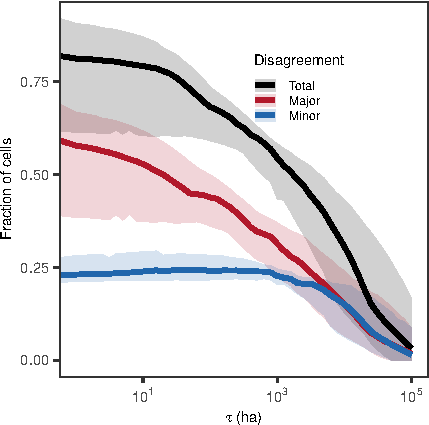
\includegraphics[keepaspectratio]{code_detectability_irrigated_areas_files/figure-latex/plot_uasa-1.pdf}}

\begin{Shaded}
\begin{Highlighting}[]
\CommentTok{\# Set colors for existential and marginal disagreement {-}{-}{-}{-}{-}{-}{-}{-}{-}{-}{-}{-}{-}{-}{-}{-}{-}{-}{-}{-}{-}{-}{-}{-}{-}}

\NormalTok{exist\_cols }\OtherTok{\textless{}{-}} \FunctionTok{c}\NormalTok{(}\StringTok{"share\_existence"} \OtherTok{=} \StringTok{"\#1f78b4"}\NormalTok{, }\StringTok{"share\_marginal"} \OtherTok{=} \StringTok{"\#e66101"}\NormalTok{)}

\NormalTok{plot\_agreement1 }\OtherTok{\textless{}{-}}\NormalTok{ mat\_sum[agreement }\SpecialCharTok{\%in\%} \FunctionTok{c}\NormalTok{(}\StringTok{"share\_existence"}\NormalTok{, }\StringTok{"share\_marginal"}\NormalTok{)] }\SpecialCharTok{\%\textgreater{}\%}
  \FunctionTok{ggplot}\NormalTok{(., }\FunctionTok{aes}\NormalTok{(}\AttributeTok{x =}\NormalTok{ tau, }\AttributeTok{y =}\NormalTok{ frac\_median, }\AttributeTok{colour =}\NormalTok{ agreement, }\AttributeTok{fill =}\NormalTok{ agreement)) }\SpecialCharTok{+}
  \FunctionTok{geom\_ribbon}\NormalTok{(}\FunctionTok{aes}\NormalTok{(}\AttributeTok{ymin =}\NormalTok{ frac\_lwr, }\AttributeTok{ymax =}\NormalTok{ frac\_upr), }\AttributeTok{alpha =} \FloatTok{0.18}\NormalTok{, }\AttributeTok{colour =} \ConstantTok{NA}\NormalTok{) }\SpecialCharTok{+}
  \FunctionTok{geom\_line}\NormalTok{(}\AttributeTok{linewidth =} \FloatTok{1.1}\NormalTok{) }\SpecialCharTok{+}
  \FunctionTok{scale\_colour\_manual}\NormalTok{(}\AttributeTok{values =}\NormalTok{ exist\_cols,}
                      \AttributeTok{labels =} \FunctionTok{c}\NormalTok{(}\AttributeTok{share\_existence =} \StringTok{"Existential"}\NormalTok{,}
                                 \AttributeTok{share\_marginal =} \StringTok{"Marginal"}\NormalTok{),}
                      \AttributeTok{name =} \StringTok{"Disagreement"}\NormalTok{) }\SpecialCharTok{+}
  \FunctionTok{scale\_fill\_manual}\NormalTok{(}\AttributeTok{values =}\NormalTok{ exist\_cols,}
                    \AttributeTok{labels =} \FunctionTok{c}\NormalTok{(}\AttributeTok{share\_existence =} \StringTok{"Existential"}\NormalTok{,}
                               \AttributeTok{share\_marginal =} \StringTok{"Marginal"}\NormalTok{),}
                    \AttributeTok{name =} \StringTok{"Disagreement"}\NormalTok{) }\SpecialCharTok{+}
  \FunctionTok{scale\_x\_log10}\NormalTok{(}\AttributeTok{labels =} \FunctionTok{label\_log}\NormalTok{(}\AttributeTok{digits =} \DecValTok{2}\NormalTok{)) }\SpecialCharTok{+}
  \FunctionTok{labs}\NormalTok{(}\AttributeTok{x =} \FunctionTok{expression}\NormalTok{(tau}\SpecialCharTok{\textasciitilde{}}\StringTok{"(ha)"}\NormalTok{), }\AttributeTok{y =} \StringTok{"Fraction of cells"}\NormalTok{) }\SpecialCharTok{+}
  \FunctionTok{theme\_AP}\NormalTok{() }\SpecialCharTok{+}
  \FunctionTok{theme}\NormalTok{(}\AttributeTok{legend.position =} \FunctionTok{c}\NormalTok{(}\FloatTok{0.3}\NormalTok{, }\FloatTok{0.7}\NormalTok{))}


\NormalTok{plot\_agreement1}
\end{Highlighting}
\end{Shaded}

\begin{verbatim}
## Warning in scale_x_log10(labels = label_log(digits = 2)): log-10 transformation introduced infinite values.
## log-10 transformation introduced infinite values.
\end{verbatim}

\pandocbounded{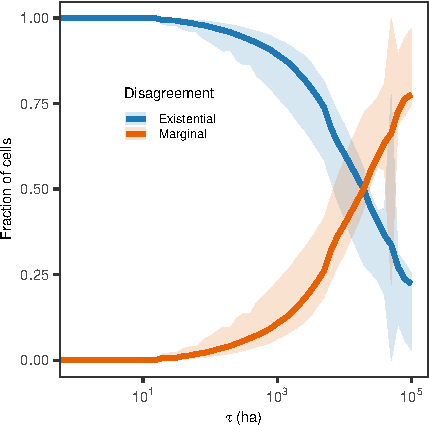
\includegraphics[keepaspectratio]{code_detectability_irrigated_areas_files/figure-latex/plot_uasa-2.pdf}}

\begin{Shaded}
\begin{Highlighting}[]
\CommentTok{\# Around tau \textgreater{} 10\^{}4 ha, the existential and marginal components intersect. That }
\CommentTok{\# intersection has a clear conceptual meaning:}
\CommentTok{\# {-}It is the tolerance level at which disagreement about whether irrigation exists}
\CommentTok{\# at all becomes less dominant than disagreement about how much irrigation exists.}
\CommentTok{\# {-}Still small relative to grid{-}cell area. 1000 ha is only 2–3\% of a 0.2º grid cell. }
\CommentTok{\# That makes it a conservative tolerance as we are not allowing massive within{-}cell }
\CommentTok{\# divergence.}

\CommentTok{\# SENSITIVITY ANALYSIS \#\#\#\#\#\#\#\#\#\#\#\#\#\#\#\#\#\#\#\#\#\#\#\#\#\#\#\#\#\#\#\#\#\#\#\#\#\#\#\#\#\#\#\#\#\#\#\#\#\#\#\#\#\#\#\#\#}

\CommentTok{\# Sobol\textquotesingle{} indices {-}{-}{-}{-}{-}{-}{-}{-}{-}{-}{-}{-}{-}{-}{-}{-}{-}{-}{-}{-}{-}{-}{-}{-}{-}{-}{-}{-}{-}{-}{-}{-}{-}{-}{-}{-}{-}{-}{-}{-}{-}{-}{-}{-}{-}{-}{-}{-}{-}{-}{-}{-}{-}{-}{-}{-}{-}{-}{-}{-}{-}{-}{-}}

\NormalTok{ind }\OtherTok{\textless{}{-}} \FunctionTok{sobol\_indices}\NormalTok{(}\AttributeTok{matrices =}\NormalTok{ matrices, }\AttributeTok{N =}\NormalTok{ N, }\AttributeTok{params =}\NormalTok{ params, Y}
                     \OtherTok{=}\NormalTok{ mat[, frac\_disagree], }\AttributeTok{R =}\NormalTok{ R, }\AttributeTok{boot =} \ConstantTok{TRUE}\NormalTok{)}

\FunctionTok{print}\NormalTok{(ind)}
\end{Highlighting}
\end{Shaded}

\begin{verbatim}
## 
## First-order estimator: saltelli | Total-order estimator: jansen 
## 
## Total number of model runs: 40960 
## 
## Sum of first order indices: 0.904819 
##        original          bias   std.error        low.ci     high.ci sensitivity
##           <num>         <num>       <num>         <num>       <num>      <char>
## 1: 0.0007484542  4.417372e-04 0.011660047 -0.0225465550 0.023159989          Si
## 2: 0.8967941330 -1.498522e-03 0.031388070  0.8367731675 0.959812143          Si
## 3: 0.0072764404  9.392697e-06 0.003397146  0.0006087643 0.013925331          Si
## 4: 0.0950335346 -8.057155e-05 0.001700313  0.0917815541 0.098446658          Ti
## 5: 0.9926671642 -5.217228e-04 0.013272194  0.9671758657 1.019201908          Ti
## 6: 0.0084121795  5.740038e-07 0.000177855  0.0080630161 0.008760195          Ti
##    parameters
##        <char>
## 1: resolution
## 2:        tau
## 3:  exclusion
## 4: resolution
## 5:        tau
## 6:  exclusion
\end{verbatim}

\begin{Shaded}
\begin{Highlighting}[]
\NormalTok{plot\_indices1 }\OtherTok{\textless{}{-}} \FunctionTok{plot}\NormalTok{(ind) }\SpecialCharTok{+}
  \FunctionTok{labs}\NormalTok{(}\AttributeTok{x =} \StringTok{""}\NormalTok{, }\AttributeTok{y =} \StringTok{"Fraction of variance"}\NormalTok{) }\SpecialCharTok{+}
  \FunctionTok{theme\_AP}\NormalTok{() }\SpecialCharTok{+}
  \FunctionTok{scale\_x\_discrete}\NormalTok{(}\AttributeTok{labels =} \FunctionTok{c}\NormalTok{(}\AttributeTok{exclusion =} \StringTok{"exclusion"}\NormalTok{,}
                              \AttributeTok{resolution =} \StringTok{"resolution"}\NormalTok{,}
                              \AttributeTok{tau =} \FunctionTok{expression}\NormalTok{(tau)),}
                   \AttributeTok{guide =} \FunctionTok{guide\_axis}\NormalTok{(}\AttributeTok{n.dodge =} \DecValTok{2}\NormalTok{)) }\SpecialCharTok{+}
  \FunctionTok{theme}\NormalTok{(}\AttributeTok{legend.position =} \FunctionTok{c}\NormalTok{(}\FloatTok{0.3}\NormalTok{, }\FloatTok{0.8}\NormalTok{))}

\NormalTok{plot\_indices1}
\end{Highlighting}
\end{Shaded}

\pandocbounded{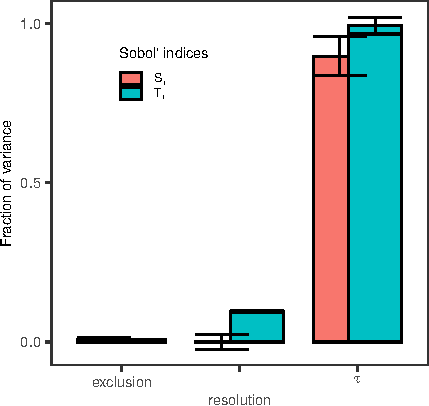
\includegraphics[keepaspectratio]{code_detectability_irrigated_areas_files/figure-latex/plot_uasa-3.pdf}}

\begin{Shaded}
\begin{Highlighting}[]
\CommentTok{\# SCATTERPLOTS OF OUTPUT AGAINS INTPUT \#\#\#\#\#\#\#\#\#\#\#\#\#\#\#\#\#\#\#\#\#\#\#\#\#\#\#\#\#\#\#\#\#\#\#\#\#\#\#\#\#}

\NormalTok{label\_map }\OtherTok{\textless{}{-}} \FunctionTok{setNames}\NormalTok{(new\_dataset\_names, dataset\_names)}

\NormalTok{a1 }\OtherTok{\textless{}{-}} \FunctionTok{ggplot}\NormalTok{(mat[}\SpecialCharTok{!}\NormalTok{exclusion }\SpecialCharTok{==} \StringTok{"all"}\NormalTok{, }\FunctionTok{c}\NormalTok{(}\StringTok{"exclusion"}\NormalTok{, }\StringTok{"frac\_disagree"}\NormalTok{)],}
            \FunctionTok{aes}\NormalTok{(exclusion, frac\_disagree)) }\SpecialCharTok{+}
  \FunctionTok{geom\_boxplot}\NormalTok{() }\SpecialCharTok{+}
  \FunctionTok{stat\_summary\_bin}\NormalTok{(}\AttributeTok{fun =} \StringTok{"mean"}\NormalTok{, }\AttributeTok{geom =} \StringTok{"point"}\NormalTok{,}
                   \AttributeTok{colour =} \StringTok{"red"}\NormalTok{, }\AttributeTok{size =} \DecValTok{1}\NormalTok{) }\SpecialCharTok{+}
  \FunctionTok{scale\_x\_discrete}\NormalTok{(}\AttributeTok{labels =}\NormalTok{ label\_map) }\SpecialCharTok{+}
  \FunctionTok{scale\_y\_continuous}\NormalTok{(}\AttributeTok{breaks =} \FunctionTok{breaks\_pretty}\NormalTok{(}\AttributeTok{n =} \DecValTok{3}\NormalTok{)) }\SpecialCharTok{+}
  \FunctionTok{theme\_AP}\NormalTok{() }\SpecialCharTok{+}
  \FunctionTok{theme}\NormalTok{(}\AttributeTok{axis.text.x =} \FunctionTok{element\_text}\NormalTok{(}\AttributeTok{angle =} \DecValTok{45}\NormalTok{, }\AttributeTok{hjust =} \DecValTok{1}\NormalTok{)) }\SpecialCharTok{+}
  \FunctionTok{labs}\NormalTok{(}\AttributeTok{x =} \StringTok{"exclusion"}\NormalTok{, }\AttributeTok{y =} \StringTok{"Fraction disagree"}\NormalTok{)}

\NormalTok{a1}
\end{Highlighting}
\end{Shaded}

\pandocbounded{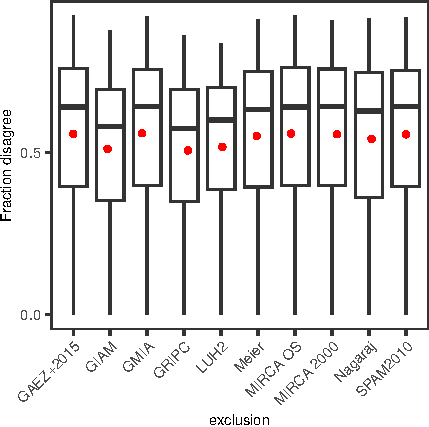
\includegraphics[keepaspectratio]{code_detectability_irrigated_areas_files/figure-latex/plot_uasa-4.pdf}}

\begin{Shaded}
\begin{Highlighting}[]
\NormalTok{b1 }\OtherTok{\textless{}{-}} \FunctionTok{ggplot}\NormalTok{(mat[}\DecValTok{1}\SpecialCharTok{:}\NormalTok{N, }\FunctionTok{c}\NormalTok{(}\StringTok{"resolution"}\NormalTok{, }\StringTok{"frac\_disagree"}\NormalTok{)],}
       \FunctionTok{aes}\NormalTok{(resolution, frac\_disagree)) }\SpecialCharTok{+}
  \FunctionTok{geom\_boxplot}\NormalTok{() }\SpecialCharTok{+}
  \FunctionTok{scale\_x\_discrete}\NormalTok{(}\AttributeTok{labels =} \FunctionTok{c}\NormalTok{(}\StringTok{\textasciigrave{}}\AttributeTok{0.2deg}\StringTok{\textasciigrave{}} \OtherTok{=} \StringTok{"0.2º"}\NormalTok{,}
                              \StringTok{\textasciigrave{}}\AttributeTok{0.4deg}\StringTok{\textasciigrave{}} \OtherTok{=} \StringTok{"0.4º"}\NormalTok{,}
                              \StringTok{\textasciigrave{}}\AttributeTok{1deg}\StringTok{\textasciigrave{}} \OtherTok{=} \StringTok{"1.0º"}\NormalTok{)) }\SpecialCharTok{+}
  \FunctionTok{scale\_y\_continuous}\NormalTok{(}\AttributeTok{breaks =} \FunctionTok{breaks\_pretty}\NormalTok{(}\AttributeTok{n =} \DecValTok{3}\NormalTok{)) }\SpecialCharTok{+}
  \FunctionTok{stat\_summary\_bin}\NormalTok{(}\AttributeTok{fun =} \StringTok{"mean"}\NormalTok{, }\AttributeTok{geom =} \StringTok{"point"}\NormalTok{,}
                   \AttributeTok{colour =} \StringTok{"red"}\NormalTok{, }\AttributeTok{size =} \DecValTok{1}\NormalTok{) }\SpecialCharTok{+}
  \FunctionTok{theme\_AP}\NormalTok{() }\SpecialCharTok{+}
  \FunctionTok{labs}\NormalTok{(}\AttributeTok{x =} \StringTok{"resolution"}\NormalTok{, }\AttributeTok{y =} \StringTok{""}\NormalTok{)}

\NormalTok{b1}
\end{Highlighting}
\end{Shaded}

\pandocbounded{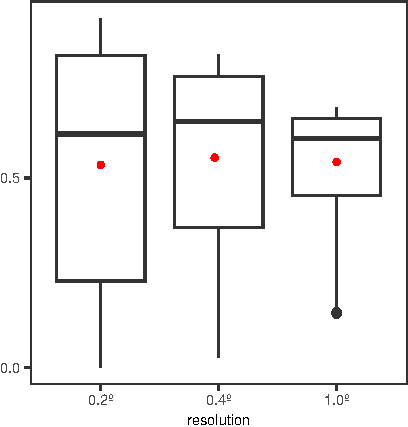
\includegraphics[keepaspectratio]{code_detectability_irrigated_areas_files/figure-latex/plot_uasa-5.pdf}}

\begin{Shaded}
\begin{Highlighting}[]
\NormalTok{c1 }\OtherTok{\textless{}{-}} \FunctionTok{ggplot}\NormalTok{(mat[}\DecValTok{1}\SpecialCharTok{:}\NormalTok{N, }\FunctionTok{c}\NormalTok{(}\StringTok{"tau"}\NormalTok{, }\StringTok{"frac\_disagree"}\NormalTok{)],}
       \FunctionTok{aes}\NormalTok{(tau, frac\_disagree)) }\SpecialCharTok{+}
  \FunctionTok{geom\_point}\NormalTok{(}\AttributeTok{size =} \FloatTok{0.1}\NormalTok{, }\AttributeTok{alpha =} \FloatTok{0.1}\NormalTok{) }\SpecialCharTok{+}
  \FunctionTok{stat\_summary\_bin}\NormalTok{(}\AttributeTok{fun =} \StringTok{"mean"}\NormalTok{, }\AttributeTok{geom =} \StringTok{"point"}\NormalTok{,}
                   \AttributeTok{colour =} \StringTok{"red"}\NormalTok{, }\AttributeTok{size =} \DecValTok{1}\NormalTok{) }\SpecialCharTok{+}
  \FunctionTok{scale\_y\_continuous}\NormalTok{(}\AttributeTok{breaks =} \FunctionTok{breaks\_pretty}\NormalTok{(}\AttributeTok{n =} \DecValTok{3}\NormalTok{)) }\SpecialCharTok{+}
  \FunctionTok{theme\_AP}\NormalTok{() }\SpecialCharTok{+}
  \FunctionTok{scale\_x\_log10}\NormalTok{(}\AttributeTok{labels =} \FunctionTok{label\_log}\NormalTok{(}\AttributeTok{digits =} \DecValTok{2}\NormalTok{)) }\SpecialCharTok{+}
  \FunctionTok{labs}\NormalTok{(}\AttributeTok{x =} \FunctionTok{expression}\NormalTok{(tau}\SpecialCharTok{\textasciitilde{}}\StringTok{"(ha)"}\NormalTok{), }\AttributeTok{y =} \StringTok{""}\NormalTok{)}

\NormalTok{c1}
\end{Highlighting}
\end{Shaded}

\begin{verbatim}
## Warning in scale_x_log10(labels = label_log(digits = 2)): log-10 transformation introduced infinite values.
## log-10 transformation introduced infinite values.
\end{verbatim}

\begin{verbatim}
## Warning: Removed 157 rows containing non-finite outside the scale range
## (`stat_summary_bin()`).
\end{verbatim}

\pandocbounded{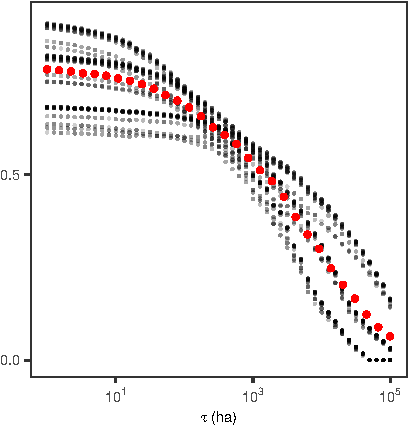
\includegraphics[keepaspectratio]{code_detectability_irrigated_areas_files/figure-latex/plot_uasa-6.pdf}}

\begin{Shaded}
\begin{Highlighting}[]
\CommentTok{\# PLOT DATASETS \#\#\#\#\#\#\#\#\#\#\#\#\#\#\#\#\#\#\#\#\#\#\#\#\#\#\#\#\#\#\#\#\#\#\#\#\#\#\#\#\#\#\#\#\#\#\#\#\#\#\#\#\#\#\#\#\#\#\#\#\#\#\#\#}

\NormalTok{tmp }\OtherTok{\textless{}{-}}\NormalTok{ dt[resolution }\SpecialCharTok{==} \StringTok{"0.2deg"}\NormalTok{] }\SpecialCharTok{\%\textgreater{}\%}
\NormalTok{  .[, .(}\AttributeTok{mha =} \FunctionTok{sum}\NormalTok{(mha)), dataset] }\SpecialCharTok{\%\textgreater{}\%}
\NormalTok{  .[, continent}\SpecialCharTok{:=} \StringTok{"GLOBAL"}\NormalTok{]}

\NormalTok{dt[resolution }\SpecialCharTok{==} \StringTok{"0.2deg"}\NormalTok{] }\SpecialCharTok{\%\textgreater{}\%}
\NormalTok{  .[, .(}\AttributeTok{mha =} \FunctionTok{sum}\NormalTok{(mha)), .(continent, dataset)] }\SpecialCharTok{\%\textgreater{}\%}
  \FunctionTok{rbind}\NormalTok{(., tmp) }\SpecialCharTok{\%\textgreater{}\%}
\NormalTok{  .[, continent}\SpecialCharTok{:=} \FunctionTok{factor}\NormalTok{(continent, }\AttributeTok{levels =} \FunctionTok{c}\NormalTok{(}\StringTok{"Africa"}\NormalTok{, }\StringTok{"Americas"}\NormalTok{,}
                                               \StringTok{"Asia"}\NormalTok{, }\StringTok{"Europe"}\NormalTok{, }\StringTok{"Oceania"}\NormalTok{,}
                                               \StringTok{"GLOBAL"}\NormalTok{))] }\SpecialCharTok{\%\textgreater{}\%}
  \FunctionTok{ggplot}\NormalTok{(., }\FunctionTok{aes}\NormalTok{(dataset, mha, }\AttributeTok{fill =}\NormalTok{ dataset)) }\SpecialCharTok{+}
  \FunctionTok{geom\_bar}\NormalTok{(}\AttributeTok{stat =} \StringTok{"identity"}\NormalTok{) }\SpecialCharTok{+}
  \FunctionTok{scale\_fill\_brewer}\NormalTok{(}\AttributeTok{palette =} \StringTok{"Paired"}\NormalTok{, }\AttributeTok{label =}\NormalTok{ label\_map, }\AttributeTok{name =} \StringTok{""}\NormalTok{) }\SpecialCharTok{+}
  \FunctionTok{facet\_wrap}\NormalTok{(}\SpecialCharTok{\textasciitilde{}}\NormalTok{continent, }\AttributeTok{ncol =} \DecValTok{6}\NormalTok{, }\AttributeTok{scales =} \StringTok{"free\_y"}\NormalTok{) }\SpecialCharTok{+}
  \FunctionTok{theme\_AP}\NormalTok{() }\SpecialCharTok{+}
  \FunctionTok{labs}\NormalTok{(}\AttributeTok{x =} \StringTok{""}\NormalTok{, }\AttributeTok{y =} \StringTok{"Mha"}\NormalTok{) }\SpecialCharTok{+}
  \FunctionTok{theme}\NormalTok{(}\AttributeTok{legend.position =} \StringTok{"top"}\NormalTok{) }\SpecialCharTok{+}
  \FunctionTok{theme}\NormalTok{(}\AttributeTok{axis.text.x =} \FunctionTok{element\_blank}\NormalTok{(),}
        \AttributeTok{axis.ticks.x =} \FunctionTok{element\_blank}\NormalTok{())}
\end{Highlighting}
\end{Shaded}

\pandocbounded{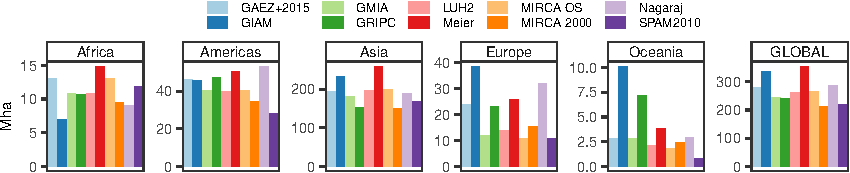
\includegraphics[keepaspectratio]{code_detectability_irrigated_areas_files/figure-latex/all_maps-1.pdf}}

\begin{Shaded}
\begin{Highlighting}[]
\CommentTok{\# MERGE UA/SA PLOTS \#\#\#\#\#\#\#\#\#\#\#\#\#\#\#\#\#\#\#\#\#\#\#\#\#\#\#\#\#\#\#\#\#\#\#\#\#\#\#\#\#\#\#\#\#\#\#\#\#\#\#\#\#\#\#\#\#\#\#\#}

\NormalTok{top }\OtherTok{\textless{}{-}} \FunctionTok{plot\_grid}\NormalTok{(plot\_uncertainty1, plot\_agreement1, plot\_indices1,}
                 \AttributeTok{ncol =} \DecValTok{3}\NormalTok{, }\AttributeTok{labels =} \StringTok{"auto"}\NormalTok{, }\AttributeTok{rel\_widths =} \FunctionTok{c}\NormalTok{(}\FloatTok{0.4}\NormalTok{, }\FloatTok{0.3}\NormalTok{, }\FloatTok{0.3}\NormalTok{))}
\end{Highlighting}
\end{Shaded}

\begin{verbatim}
## Warning in scale_x_log10(labels = label_log(digits = 2)): log-10 transformation introduced infinite values.
## log-10 transformation introduced infinite values.
## log-10 transformation introduced infinite values.
## log-10 transformation introduced infinite values.
\end{verbatim}

\begin{Shaded}
\begin{Highlighting}[]
\NormalTok{bottom }\OtherTok{\textless{}{-}} \FunctionTok{plot\_grid}\NormalTok{(a1, b1, c1, }\AttributeTok{ncol =} \DecValTok{3}\NormalTok{, }\AttributeTok{rel\_widths =} \FunctionTok{c}\NormalTok{(}\FloatTok{0.5}\NormalTok{, }\FloatTok{0.25}\NormalTok{, }\FloatTok{0.25}\NormalTok{), }\AttributeTok{labels =} \StringTok{"d"}\NormalTok{)}
\end{Highlighting}
\end{Shaded}

\begin{verbatim}
## Warning in scale_x_log10(labels = label_log(digits = 2)): log-10 transformation introduced infinite values.
## log-10 transformation introduced infinite values.
\end{verbatim}

\begin{verbatim}
## Warning: Removed 157 rows containing non-finite outside the scale range
## (`stat_summary_bin()`).
\end{verbatim}

\begin{Shaded}
\begin{Highlighting}[]
\FunctionTok{plot\_grid}\NormalTok{(top, bottom, }\AttributeTok{ncol =} \DecValTok{1}\NormalTok{)}
\end{Highlighting}
\end{Shaded}

\pandocbounded{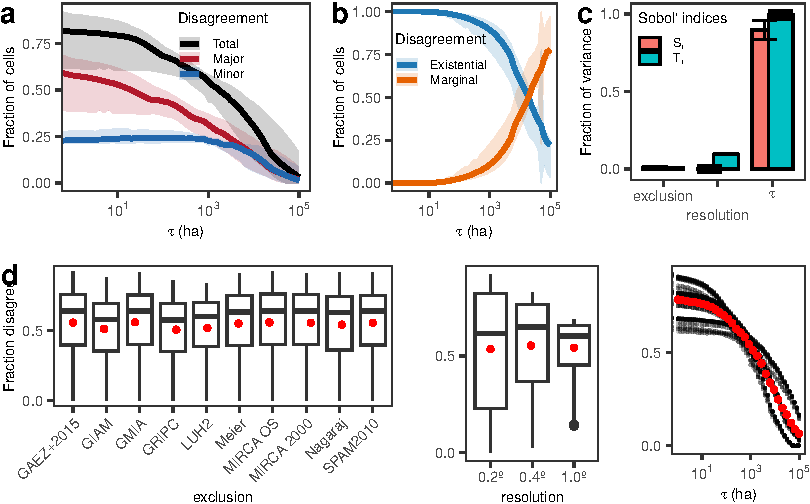
\includegraphics[keepaspectratio]{code_detectability_irrigated_areas_files/figure-latex/merge_uasa-1.pdf}}

\subsection{Does coarsening reduce
disagreement?}\label{does-coarsening-reduce-disagreement}

\begin{Shaded}
\begin{Highlighting}[]
\CommentTok{\# DOES ZOOMING OUT REDUCE DISAGREEMENT? \#\#\#\#\#\#\#\#\#\#\#\#\#\#\#\#\#\#\#\#\#\#\#\#\#\#\#\#\#\#\#\#\#\#\#\#\#\#\#\#}

\NormalTok{effect\_resolution\_dt }\OtherTok{\textless{}{-}}\NormalTok{ tau\_results[scenario }\SpecialCharTok{==} \StringTok{"all"}\NormalTok{, .(tau, frac\_disagree, resolution)]}

\CommentTok{\# Order resolution {-}{-}{-}{-}{-}{-}{-}{-}{-}{-}{-}{-}{-}{-}{-}{-}{-}{-}{-}{-}{-}{-}{-}{-}{-}{-}{-}{-}{-}{-}{-}{-}{-}{-}{-}{-}{-}{-}{-}{-}{-}{-}{-}{-}{-}{-}{-}{-}{-}{-}{-}{-}{-}{-}{-}{-}{-}{-}{-}{-}{-}}

\NormalTok{effect\_resolution\_dt[, resolution}\SpecialCharTok{:=} \FunctionTok{factor}\NormalTok{(resolution,}
                                           \AttributeTok{levels =} \FunctionTok{c}\NormalTok{(}\StringTok{"0.2deg"}\NormalTok{, }\StringTok{"0.4deg"}\NormalTok{, }\StringTok{"1deg"}\NormalTok{))]}

\CommentTok{\# To wide table {-}{-}{-}{-}{-}{-}{-}{-}{-}{-}{-}{-}{-}{-}{-}{-}{-}{-}{-}{-}{-}{-}{-}{-}{-}{-}{-}{-}{-}{-}{-}{-}{-}{-}{-}{-}{-}{-}{-}{-}{-}{-}{-}{-}{-}{-}{-}{-}{-}{-}{-}{-}{-}{-}{-}{-}{-}{-}{-}{-}{-}{-}{-}{-}}

\NormalTok{wide\_dt }\OtherTok{\textless{}{-}} \FunctionTok{dcast}\NormalTok{(effect\_resolution\_dt, tau }\SpecialCharTok{\textasciitilde{}}\NormalTok{ resolution, }\AttributeTok{value.var =} \StringTok{"frac\_disagree"}\NormalTok{)}

\CommentTok{\# Rename {-}{-}{-}{-}{-}{-}{-}{-}{-}{-}{-}{-}{-}{-}{-}{-}{-}{-}{-}{-}{-}{-}{-}{-}{-}{-}{-}{-}{-}{-}{-}{-}{-}{-}{-}{-}{-}{-}{-}{-}{-}{-}{-}{-}{-}{-}{-}{-}{-}{-}{-}{-}{-}{-}{-}{-}{-}{-}{-}{-}{-}{-}{-}{-}{-}{-}{-}{-}{-}{-}{-}}

\FunctionTok{setnames}\NormalTok{(wide\_dt, }\AttributeTok{old =} \FunctionTok{c}\NormalTok{(}\StringTok{"0.2deg"}\NormalTok{, }\StringTok{"0.4deg"}\NormalTok{, }\StringTok{"1deg"}\NormalTok{), }\AttributeTok{new =} \FunctionTok{c}\NormalTok{(}\StringTok{"res\_0.2"}\NormalTok{, }\StringTok{"res\_0.4"}\NormalTok{, }\StringTok{"res\_1"}\NormalTok{))}

\CommentTok{\# Compute absolute change (fine {-} coarse) {-}{-}{-}{-}{-}{-}{-}{-}{-}{-}{-}{-}{-}{-}{-}{-}{-}{-}{-}{-}{-}{-}{-}{-}{-}{-}{-}{-}{-}{-}{-}{-}{-}{-}{-}{-}{-}{-}}

\NormalTok{wide\_dt[, abs\_change}\SpecialCharTok{:=}\NormalTok{ res\_0}\FloatTok{.2} \SpecialCharTok{{-}}\NormalTok{ res\_1]}

\CommentTok{\# Compute elasticity (log{-}log) {-}{-}{-}{-}{-}{-}{-}{-}{-}{-}{-}{-}{-}{-}{-}{-}{-}{-}{-}{-}{-}{-}{-}{-}{-}{-}{-}{-}{-}{-}{-}{-}{-}{-}{-}{-}{-}{-}{-}{-}{-}{-}{-}{-}{-}{-}{-}{-}{-}}

\CommentTok{\# Area ratio from 0.2 to 1}
\NormalTok{area\_ratio }\OtherTok{\textless{}{-}} \DecValTok{25}
\NormalTok{wide\_dt[, elasticity}\SpecialCharTok{:=} \FunctionTok{ifelse}\NormalTok{(res\_0}\FloatTok{.2} \SpecialCharTok{\textgreater{}} \DecValTok{0} \SpecialCharTok{\&}\NormalTok{ res\_1 }\SpecialCharTok{\textgreater{}} \DecValTok{0}\NormalTok{,}
                              \FunctionTok{log}\NormalTok{(res\_1 }\SpecialCharTok{/}\NormalTok{ res\_0}\FloatTok{.2}\NormalTok{) }\SpecialCharTok{/} \FunctionTok{log}\NormalTok{(area\_ratio), }\ConstantTok{NA\_real\_}\NormalTok{)]}

\CommentTok{\# Plot disagreement curves {-}{-}{-}{-}{-}{-}{-}{-}{-}{-}{-}{-}{-}{-}{-}{-}{-}{-}{-}{-}{-}{-}{-}{-}{-}{-}{-}{-}{-}{-}{-}{-}{-}{-}{-}{-}{-}{-}{-}{-}{-}{-}{-}{-}{-}{-}{-}{-}{-}{-}{-}{-}{-}}

\NormalTok{p1 }\OtherTok{\textless{}{-}} \FunctionTok{ggplot}\NormalTok{(effect\_resolution\_dt, }\FunctionTok{aes}\NormalTok{(tau, frac\_disagree, }\AttributeTok{colour =}\NormalTok{ resolution)) }\SpecialCharTok{+}
  \FunctionTok{geom\_line}\NormalTok{(}\AttributeTok{linewidth =} \FloatTok{0.8}\NormalTok{) }\SpecialCharTok{+}
  \FunctionTok{scale\_x\_log10}\NormalTok{(}\AttributeTok{labels =} \FunctionTok{label\_log}\NormalTok{(}\AttributeTok{digits =} \DecValTok{2}\NormalTok{)) }\SpecialCharTok{+}
  \FunctionTok{scale\_color\_manual}\NormalTok{(}\AttributeTok{values =}\NormalTok{ res\_palette) }\SpecialCharTok{+}
  \FunctionTok{labs}\NormalTok{(}\AttributeTok{x =} \FunctionTok{expression}\NormalTok{(tau}\SpecialCharTok{\textasciitilde{}}\StringTok{"(ha)"}\NormalTok{),}
       \AttributeTok{y =} \StringTok{"Fraction of cells"}\NormalTok{,}
       \AttributeTok{colour =} \StringTok{"Resolution"}\NormalTok{) }\SpecialCharTok{+}
  \FunctionTok{theme\_AP}\NormalTok{() }\SpecialCharTok{+}
  \FunctionTok{theme}\NormalTok{(}\AttributeTok{legend.position =} \FunctionTok{c}\NormalTok{(}\FloatTok{0.3}\NormalTok{, }\FloatTok{0.35}\NormalTok{))}

\NormalTok{p1}
\end{Highlighting}
\end{Shaded}

\begin{verbatim}
## Warning in scale_x_log10(labels = label_log(digits = 2)): log-10 transformation
## introduced infinite values.
\end{verbatim}

\pandocbounded{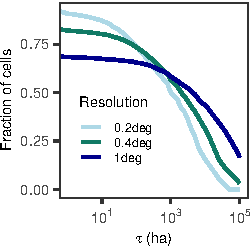
\includegraphics[keepaspectratio]{code_detectability_irrigated_areas_files/figure-latex/effects_coarsening-1.pdf}}

\begin{Shaded}
\begin{Highlighting}[]
\CommentTok{\# Plot absolute change {-}{-}{-}{-}{-}{-}{-}{-}{-}{-}{-}{-}{-}{-}{-}{-}{-}{-}{-}{-}{-}{-}{-}{-}{-}{-}{-}{-}{-}{-}{-}{-}{-}{-}{-}{-}{-}{-}{-}{-}{-}{-}{-}{-}{-}{-}{-}{-}{-}{-}{-}{-}{-}{-}{-}{-}{-}}

\NormalTok{p2 }\OtherTok{\textless{}{-}} \FunctionTok{ggplot}\NormalTok{(wide\_dt, }\FunctionTok{aes}\NormalTok{(tau, abs\_change)) }\SpecialCharTok{+}
  \FunctionTok{geom\_hline}\NormalTok{(}\AttributeTok{yintercept =} \DecValTok{0}\NormalTok{, }\AttributeTok{linetype =} \StringTok{"dashed"}\NormalTok{) }\SpecialCharTok{+}
  \FunctionTok{geom\_line}\NormalTok{(}\AttributeTok{linewidth =} \FloatTok{0.8}\NormalTok{) }\SpecialCharTok{+}
  \FunctionTok{scale\_x\_log10}\NormalTok{(}\AttributeTok{labels =} \FunctionTok{label\_log}\NormalTok{(}\AttributeTok{digits =} \DecValTok{2}\NormalTok{)) }\SpecialCharTok{+}
  \FunctionTok{labs}\NormalTok{(}\AttributeTok{x =} \FunctionTok{expression}\NormalTok{(tau}\SpecialCharTok{\textasciitilde{}}\StringTok{"(ha)"}\NormalTok{),}
       \AttributeTok{y =} \StringTok{"Change disagreement"}\NormalTok{) }\SpecialCharTok{+}
  \FunctionTok{theme\_AP}\NormalTok{()}

\NormalTok{p2}
\end{Highlighting}
\end{Shaded}

\begin{verbatim}
## Warning in scale_x_log10(labels = label_log(digits = 2)): log-10 transformation
## introduced infinite values.
\end{verbatim}

\pandocbounded{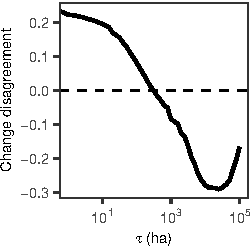
\includegraphics[keepaspectratio]{code_detectability_irrigated_areas_files/figure-latex/effects_coarsening-2.pdf}}

\begin{Shaded}
\begin{Highlighting}[]
\CommentTok{\# Plot elasticity {-}{-}{-}{-}{-}{-}{-}{-}{-}{-}{-}{-}{-}{-}{-}{-}{-}{-}{-}{-}{-}{-}{-}{-}{-}{-}{-}{-}{-}{-}{-}{-}{-}{-}{-}{-}{-}{-}{-}{-}{-}{-}{-}{-}{-}{-}{-}{-}{-}{-}{-}{-}{-}{-}{-}{-}{-}{-}{-}{-}{-}{-}}

\NormalTok{p3 }\OtherTok{\textless{}{-}} \FunctionTok{ggplot}\NormalTok{(wide\_dt[}\SpecialCharTok{!}\FunctionTok{is.na}\NormalTok{(elasticity)],}
       \FunctionTok{aes}\NormalTok{(}\AttributeTok{x =}\NormalTok{ tau, }\AttributeTok{y =}\NormalTok{ elasticity)) }\SpecialCharTok{+}
  \FunctionTok{geom\_hline}\NormalTok{(}\AttributeTok{yintercept =} \DecValTok{0}\NormalTok{, }\AttributeTok{linetype =} \StringTok{"dashed"}\NormalTok{) }\SpecialCharTok{+}
  \FunctionTok{geom\_line}\NormalTok{(}\AttributeTok{linewidth =} \FloatTok{0.8}\NormalTok{) }\SpecialCharTok{+}
  \FunctionTok{scale\_x\_log10}\NormalTok{(}\AttributeTok{labels =} \FunctionTok{label\_log}\NormalTok{(}\AttributeTok{digits =} \DecValTok{2}\NormalTok{)) }\SpecialCharTok{+}
  \FunctionTok{labs}\NormalTok{(}\AttributeTok{x =} \FunctionTok{expression}\NormalTok{(tau}\SpecialCharTok{\textasciitilde{}}\StringTok{"(ha)"}\NormalTok{),}
       \AttributeTok{y =} \StringTok{"Elasticity disagreement"}\NormalTok{) }\SpecialCharTok{+}
  \FunctionTok{theme\_AP}\NormalTok{()}

\NormalTok{p3}
\end{Highlighting}
\end{Shaded}

\begin{verbatim}
## Warning in scale_x_log10(labels = label_log(digits = 2)): log-10 transformation
## introduced infinite values.
\end{verbatim}

\pandocbounded{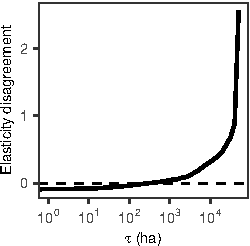
\includegraphics[keepaspectratio]{code_detectability_irrigated_areas_files/figure-latex/effects_coarsening-3.pdf}}

\begin{Shaded}
\begin{Highlighting}[]
\CommentTok{\# Merge {-}{-}{-}{-}{-}{-}{-}{-}{-}{-}{-}{-}{-}{-}{-}{-}{-}{-}{-}{-}{-}{-}{-}{-}{-}{-}{-}{-}{-}{-}{-}{-}{-}{-}{-}{-}{-}{-}{-}{-}{-}{-}{-}{-}{-}{-}{-}{-}{-}{-}{-}{-}{-}{-}{-}{-}{-}{-}{-}{-}{-}{-}{-}{-}{-}{-}{-}{-}{-}{-}{-}{-}}

\FunctionTok{plot\_grid}\NormalTok{(p1, p2, p3, }\AttributeTok{ncol =} \DecValTok{3}\NormalTok{, }\AttributeTok{labels =} \StringTok{"auto"}\NormalTok{)}
\end{Highlighting}
\end{Shaded}

\begin{verbatim}
## Warning in scale_x_log10(labels = label_log(digits = 2)): log-10 transformation introduced infinite values.
## log-10 transformation introduced infinite values.
## log-10 transformation introduced infinite values.
\end{verbatim}

\pandocbounded{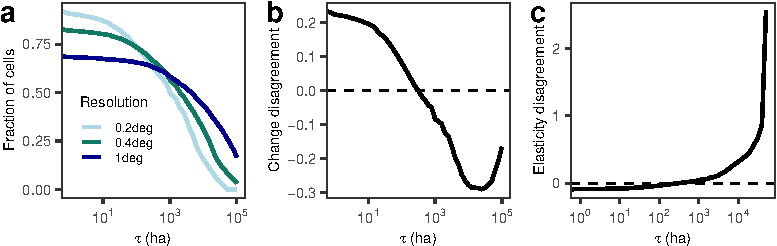
\includegraphics[keepaspectratio]{code_detectability_irrigated_areas_files/figure-latex/plot_effects_resolution-1.pdf}}

\begin{Shaded}
\begin{Highlighting}[]
\CommentTok{\# Increasing spatial aggregation from 0.2 to 1 (25x coarsening) reduces}
\CommentTok{\# existential disagreement by c20 percentage points at near{-}zero}
\CommentTok{\# thresholds. this effect vanishes around tau = 300–500 ha, beyond which}
\CommentTok{\# aggregation increases disagreement. At higher thresholds disagreement is}
\CommentTok{\# greater at 1 than at 0.2. Coarse{-}scale aggregation can}
\CommentTok{\# amplify rather than resolve structural spatial inconsistencies between datasets.}

\CommentTok{\# These results refut the criticism of "if you zoom out, the maps converge".}

\CommentTok{\# ALSO: Increasing cell area by a factor of 25 (0.2 to 1) yields an elasticity}
\CommentTok{\# of approximately {-}0.07 at tau =  0, implying that a 1\% increase in spatial}
\CommentTok{\# aggregation reduces disagreement by only 0.07\%. Elasticity approaches zero}
\CommentTok{\# at moderate thresholds and becomes positive at higher thresholds.}
\end{Highlighting}
\end{Shaded}

\newpage

\subsection{UA/SA by excluding mapping
paradigms}\label{uasa-by-excluding-mapping-paradigms}

\begin{verbatim}
##               agreement        tau    frac_mean  frac_median     frac_lwr
##                  <fctr>      <num>        <num>        <num>        <num>
##  1:       frac_disagree     0.0000 0.7614597541 0.7880460127 0.5679870856
##  2:       frac_disagree     1.0000 0.7509288549 0.7679309809 0.5623991059
##  3:       frac_disagree    10.0000 0.7294854559 0.7329727817 0.5479945362
##  4:       frac_disagree   501.1872 0.5581326448 0.5802806408 0.4333981035
##  5:       frac_disagree  1000.0000 0.4991765164 0.5359498597 0.3645422043
##  6:       frac_disagree  1584.8932 0.4667211226 0.4956152544 0.3483755635
##  7:       frac_disagree  5011.8723 0.3494441763 0.3605600344 0.2048033577
##  8:       frac_disagree 10000.0000 0.2683762710 0.2777846765 0.1081532722
##  9: frac_major_disagree     0.0000 0.5150634039 0.5083524982 0.3305600397
## 10: frac_major_disagree     1.0000 0.5002618481 0.4971063206 0.3244753508
## 11: frac_major_disagree    10.0000 0.4698033971 0.4761555763 0.3093257171
## 12: frac_major_disagree   501.1872 0.3148427241 0.3277060325 0.2023006373
## 13: frac_major_disagree  1000.0000 0.2720322427 0.2765296065 0.1730063734
## 14: frac_major_disagree  1584.8932 0.2477249872 0.2506760343 0.1598632053
## 15: frac_major_disagree  5011.8723 0.1754068622 0.1759205439 0.0926939220
## 16: frac_major_disagree 10000.0000 0.1322954415 0.1357628447 0.0536763563
## 17: frac_minor_disagree     0.0000 0.2463963501 0.2489069726 0.2139575314
## 18: frac_minor_disagree     1.0000 0.2506670067 0.2524703682 0.2180553831
## 19: frac_minor_disagree    10.0000 0.2596820587 0.2572468346 0.2227741214
## 20: frac_minor_disagree   501.1872 0.2432899207 0.2397481735 0.2108530982
## 21: frac_minor_disagree  1000.0000 0.2271442737 0.2309130885 0.1915358309
## 22: frac_minor_disagree  1584.8932 0.2189961355 0.2235191854 0.1796355733
## 23: frac_minor_disagree  5011.8723 0.1740373141 0.1727867775 0.1121094357
## 24: frac_minor_disagree 10000.0000 0.1360808295 0.1344840432 0.0544769159
## 25:     share_existence     0.0000 1.0000000000 1.0000000000 1.0000000000
## 26:     share_existence     1.0000 0.9998089324 0.9998409467 0.9995953055
## 27:     share_existence    10.0000 0.9988781627 0.9991691698 0.9974009033
## 28:     share_existence   501.1872 0.9123367031 0.9257356965 0.8303017334
## 29:     share_existence  1000.0000 0.8681909054 0.8769195082 0.7701200534
## 30:     share_existence  1584.8932 0.8330769522 0.8375351390 0.7264996553
## 31:     share_existence  5011.8723 0.6837396143 0.6927194861 0.5627427952
## 32:     share_existence 10000.0000 0.5569765612 0.5899063161 0.4023039928
## 33:      share_marginal     0.0000 0.0000000000 0.0000000000 0.0000000000
## 34:      share_marginal     1.0000 0.0001910676 0.0001590533 0.0000000000
## 35:      share_marginal    10.0000 0.0011218373 0.0008308302 0.0001593676
## 36:      share_marginal   501.1872 0.0876632969 0.0742643035 0.0389949289
## 37:      share_marginal  1000.0000 0.1318090946 0.1230804918 0.0628445947
## 38:      share_marginal  1584.8932 0.1669230478 0.1624648610 0.0804188625
## 39:      share_marginal  5011.8723 0.3162603857 0.3072805139 0.1855907949
## 40:      share_marginal 10000.0000 0.4430234388 0.4100936839 0.3128228973
##               agreement        tau    frac_mean  frac_median     frac_lwr
##                  <fctr>      <num>        <num>        <num>        <num>
##         frac_upr
##            <num>
##  1: 0.9165941240
##  2: 0.9004663454
##  3: 0.8633530235
##  4: 0.6167201597
##  5: 0.5699739228
##  6: 0.5446417484
##  7: 0.4785794114
##  8: 0.4235688563
##  9: 0.6855666097
## 10: 0.6569796363
## 11: 0.5954919944
## 12: 0.3732770396
## 13: 0.3444679002
## 14: 0.3250962374
## 15: 0.2630075748
## 16: 0.2220290575
## 17: 0.3016088917
## 18: 0.3046789989
## 19: 0.3069951811
## 20: 0.2792476294
## 21: 0.2594202532
## 22: 0.2536076221
## 23: 0.2305972929
## 24: 0.2165652552
## 25: 1.0000000000
## 26: 1.0000000000
## 27: 0.9998406324
## 28: 0.9610050711
## 29: 0.9371554053
## 30: 0.9195811375
## 31: 0.8144092051
## 32: 0.6871771027
## 33: 0.0000000000
## 34: 0.0004046945
## 35: 0.0025990967
## 36: 0.1696982666
## 37: 0.2298799466
## 38: 0.2735003447
## 39: 0.4372572048
## 40: 0.5976960072
##         frac_upr
##            <num>
\end{verbatim}

\begin{verbatim}
## Warning in scale_x_log10(labels = label_log(digits = 2)): log-10 transformation introduced infinite values.
## log-10 transformation introduced infinite values.
\end{verbatim}

\pandocbounded{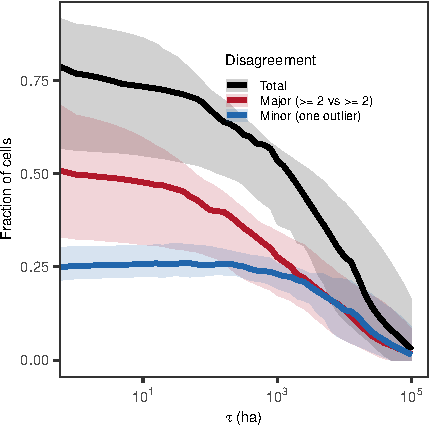
\includegraphics[keepaspectratio]{code_detectability_irrigated_areas_files/figure-latex/uasa_on_mapping_paradigm-1.pdf}}

\begin{verbatim}
## Warning in scale_x_log10(labels = label_log(digits = 2)): log-10 transformation introduced infinite values.
## log-10 transformation introduced infinite values.
\end{verbatim}

\pandocbounded{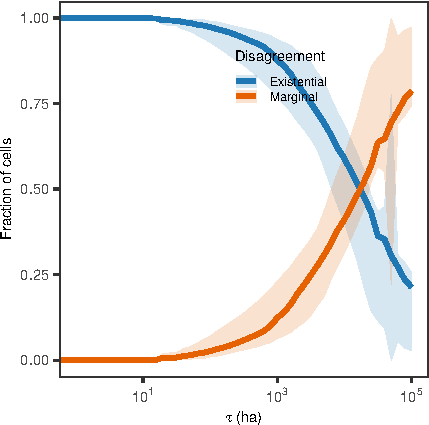
\includegraphics[keepaspectratio]{code_detectability_irrigated_areas_files/figure-latex/uasa_on_mapping_paradigm-2.pdf}}
\pandocbounded{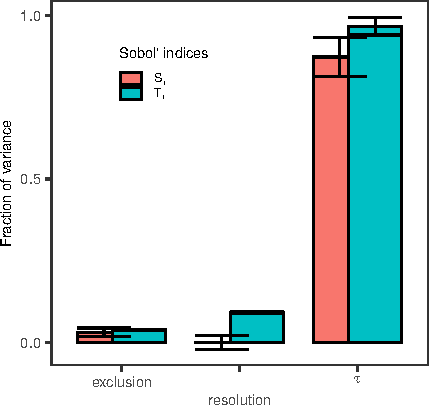
\includegraphics[keepaspectratio]{code_detectability_irrigated_areas_files/figure-latex/uasa_on_mapping_paradigm-3.pdf}}
\pandocbounded{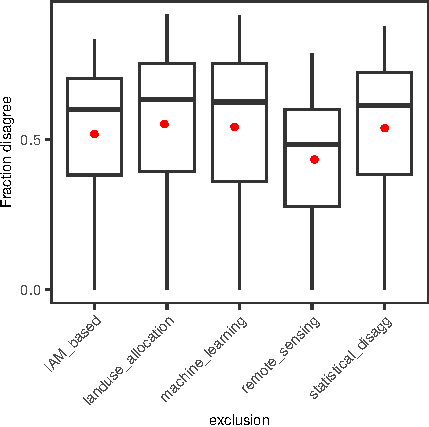
\includegraphics[keepaspectratio]{code_detectability_irrigated_areas_files/figure-latex/uasa_on_mapping_paradigm-4.pdf}}
\pandocbounded{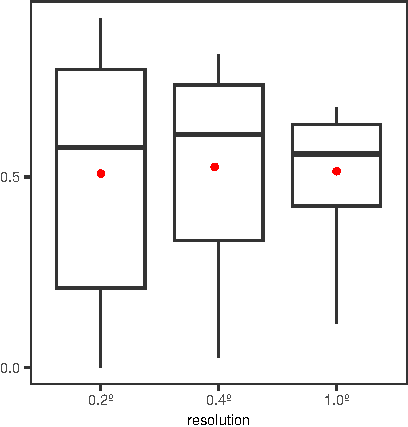
\includegraphics[keepaspectratio]{code_detectability_irrigated_areas_files/figure-latex/uasa_on_mapping_paradigm-5.pdf}}

\begin{verbatim}
## Warning in scale_x_log10(labels = label_log(digits = 2)): log-10 transformation introduced infinite values.
## log-10 transformation introduced infinite values.
\end{verbatim}

\begin{verbatim}
## Warning: Removed 157 rows containing non-finite outside the scale range
## (`stat_summary_bin()`).
\end{verbatim}

\pandocbounded{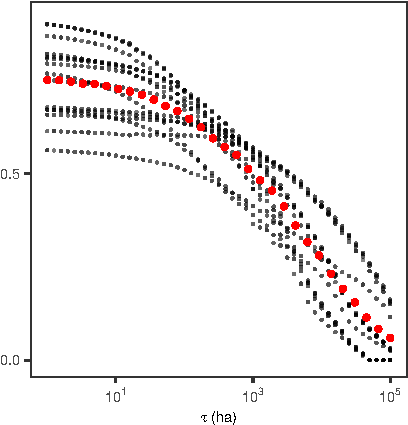
\includegraphics[keepaspectratio]{code_detectability_irrigated_areas_files/figure-latex/uasa_on_mapping_paradigm-6.pdf}}

\begin{Shaded}
\begin{Highlighting}[]
\CommentTok{\# MERGE UA/SA PLOTS \#\#\#\#\#\#\#\#\#\#\#\#\#\#\#\#\#\#\#\#\#\#\#\#\#\#\#\#\#\#\#\#\#\#\#\#\#\#\#\#\#\#\#\#\#\#\#\#\#\#\#\#\#\#\#\#\#\#\#\#}

\NormalTok{top }\OtherTok{\textless{}{-}} \FunctionTok{plot\_grid}\NormalTok{(plot\_uncertainty, plot\_agreement, plot\_indices2,}
                 \AttributeTok{ncol =} \DecValTok{3}\NormalTok{, }\AttributeTok{labels =} \StringTok{"auto"}\NormalTok{, }\AttributeTok{rel\_widths =} \FunctionTok{c}\NormalTok{(}\FloatTok{0.4}\NormalTok{, }\FloatTok{0.3}\NormalTok{, }\FloatTok{0.3}\NormalTok{))}
\end{Highlighting}
\end{Shaded}

\begin{verbatim}
## Warning in scale_x_log10(labels = label_log(digits = 2)): log-10 transformation introduced infinite values.
## log-10 transformation introduced infinite values.
## log-10 transformation introduced infinite values.
## log-10 transformation introduced infinite values.
\end{verbatim}

\begin{Shaded}
\begin{Highlighting}[]
\NormalTok{bottom }\OtherTok{\textless{}{-}} \FunctionTok{plot\_grid}\NormalTok{(a2, b2, c2, }\AttributeTok{ncol =} \DecValTok{3}\NormalTok{, }\AttributeTok{rel\_widths =} \FunctionTok{c}\NormalTok{(}\FloatTok{0.4}\NormalTok{, }\FloatTok{0.3}\NormalTok{, }\FloatTok{0.3}\NormalTok{), }\AttributeTok{labels =} \StringTok{"d"}\NormalTok{)}
\end{Highlighting}
\end{Shaded}

\begin{verbatim}
## Warning in scale_x_log10(labels = label_log(digits = 2)): log-10 transformation introduced infinite values.
## log-10 transformation introduced infinite values.
\end{verbatim}

\begin{verbatim}
## Warning: Removed 157 rows containing non-finite outside the scale range
## (`stat_summary_bin()`).
\end{verbatim}

\begin{Shaded}
\begin{Highlighting}[]
\FunctionTok{plot\_grid}\NormalTok{(top, bottom, }\AttributeTok{ncol =} \DecValTok{1}\NormalTok{)}
\end{Highlighting}
\end{Shaded}

\pandocbounded{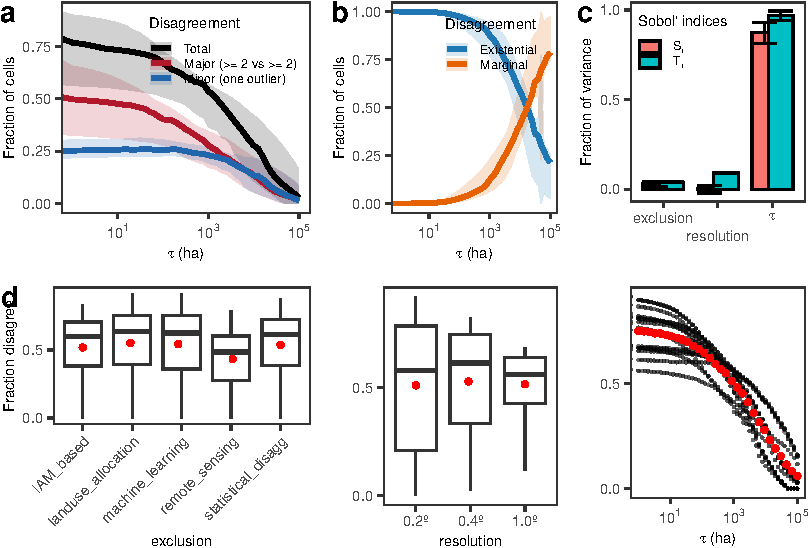
\includegraphics[keepaspectratio]{code_detectability_irrigated_areas_files/figure-latex/merge_dataset_classes-1.pdf}}

\newpage

\subsection{UA/SA by weighting newer datasets
more}\label{uasa-by-weighting-newer-datasets-more}

\begin{verbatim}
##       tau           agreement    frac_mean  frac_median     frac_lwr
##     <num>              <fctr>        <num>        <num>        <num>
##  1:    10       frac_disagree 7.613616e-01 0.7961030099 0.6052402831
##  2:   100       frac_disagree 6.861610e-01 0.6823270742 0.5909598907
##  3:     1       frac_disagree 7.835042e-01 0.8125805555 0.6136843412
##  4:     0       frac_disagree 7.906485e-01 0.8198589805 0.6172854837
##  5:  1000       frac_disagree 5.303683e-01 0.5447446233 0.4346727810
##  6:    10 frac_major_disagree 4.050533e-01 0.4085774217 0.2755494847
##  7:   100 frac_major_disagree 3.262599e-01 0.3231151873 0.2466267682
##  8:     1 frac_major_disagree 4.328001e-01 0.4348858955 0.2716999876
##  9:     0 frac_major_disagree 4.521144e-01 0.4584626847 0.2503414876
## 10:  1000 frac_major_disagree 2.145969e-01 0.2075466514 0.1478736593
## 11:    10 frac_minor_disagree 3.563083e-01 0.3468272693 0.2233950081
## 12:   100 frac_minor_disagree 3.599011e-01 0.3605853067 0.2428908481
## 13:     1 frac_minor_disagree 3.507040e-01 0.3512345523 0.2293555197
## 14:     0 frac_minor_disagree 3.385341e-01 0.3319770527 0.2325468769
## 15:  1000 frac_minor_disagree 3.157714e-01 0.3122648842 0.2535209078
## 16:    10     share_existence 9.992881e-01 0.9994458810 0.9974009033
## 17:   100     share_existence 9.705782e-01 0.9745621351 0.9296762219
## 18:     1     share_existence 9.999080e-01 0.9999382697 0.9995953055
## 19:     0     share_existence 1.000000e+00 1.0000000000 1.0000000000
## 20:  1000     share_existence 8.833496e-01 0.8929618107 0.7701200534
## 21:    10      share_marginal 7.118921e-04 0.0005541190 0.0001586546
## 22:   100      share_marginal 2.942185e-02 0.0254378649 0.0104125963
## 23:     1      share_marginal 9.198566e-05 0.0000617303 0.0000000000
## 24:     0      share_marginal 0.000000e+00 0.0000000000 0.0000000000
## 25:  1000      share_marginal 1.166504e-01 0.1070381893 0.0624304979
##       tau           agreement    frac_mean  frac_median     frac_lwr
##     <num>              <fctr>        <num>        <num>        <num>
##         frac_upr
##            <num>
##  1: 0.8713819369
##  2: 0.7371677289
##  3: 0.9071584020
##  4: 0.9215840199
##  5: 0.5832608966
##  6: 0.5214760310
##  7: 0.4238671687
##  8: 0.5695393882
##  9: 0.6142779419
## 10: 0.3214950950
## 11: 0.4568980768
## 12: 0.4307917814
## 13: 0.4665474895
## 14: 0.4576402922
## 15: 0.3688746241
## 16: 0.9998413454
## 17: 0.9895874037
## 18: 1.0000000000
## 19: 1.0000000000
## 20: 0.9375695021
## 21: 0.0025990967
## 22: 0.0703237781
## 23: 0.0004046945
## 24: 0.0000000000
## 25: 0.2298799466
##         frac_upr
##            <num>
\end{verbatim}

\begin{verbatim}
## Warning in scale_x_log10(labels = label_log(digits = 2)): log-10 transformation introduced infinite values.
## log-10 transformation introduced infinite values.
\end{verbatim}

\pandocbounded{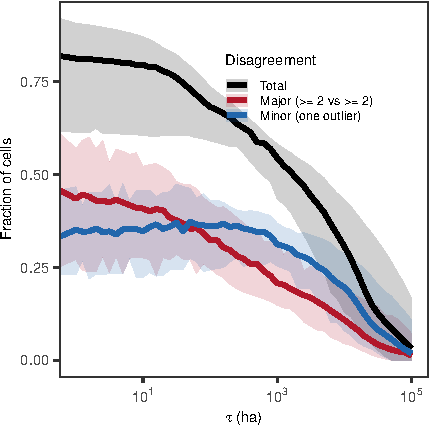
\includegraphics[keepaspectratio]{code_detectability_irrigated_areas_files/figure-latex/uasa_on_weights-1.pdf}}

\begin{verbatim}
## Warning in scale_x_log10(labels = label_log(digits = 2)): log-10 transformation introduced infinite values.
## log-10 transformation introduced infinite values.
\end{verbatim}

\pandocbounded{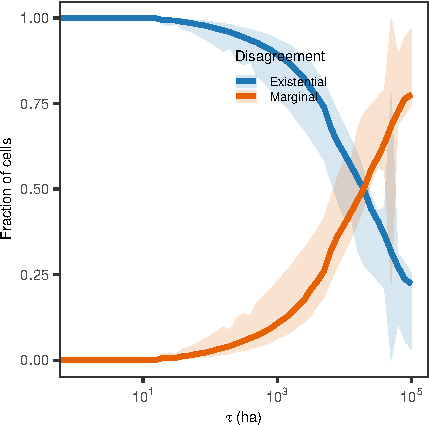
\includegraphics[keepaspectratio]{code_detectability_irrigated_areas_files/figure-latex/uasa_on_weights-2.pdf}}
\pandocbounded{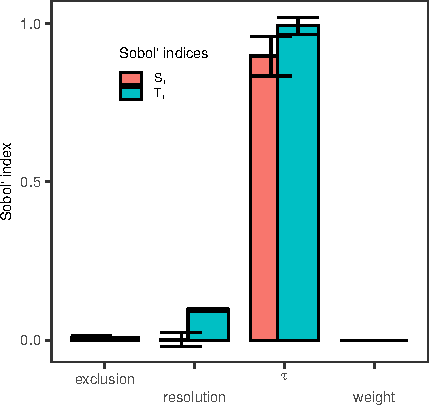
\includegraphics[keepaspectratio]{code_detectability_irrigated_areas_files/figure-latex/uasa_on_weights-3.pdf}}
\pandocbounded{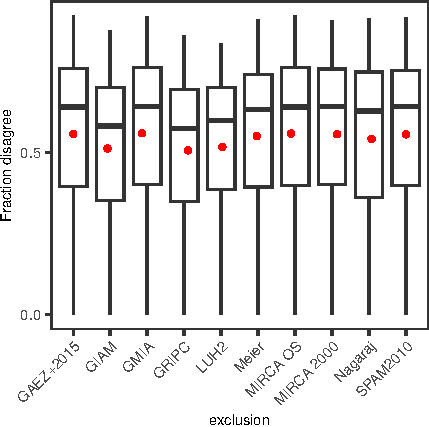
\includegraphics[keepaspectratio]{code_detectability_irrigated_areas_files/figure-latex/uasa_on_weights-4.pdf}}
\pandocbounded{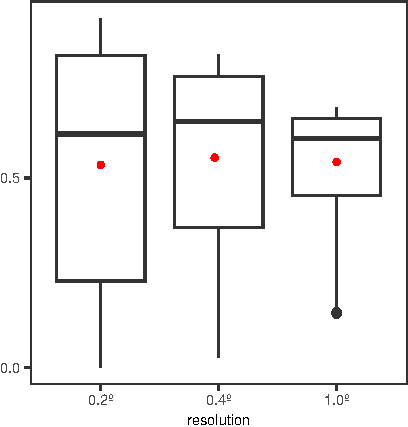
\includegraphics[keepaspectratio]{code_detectability_irrigated_areas_files/figure-latex/uasa_on_weights-5.pdf}}

\begin{verbatim}
## Warning in scale_x_log10(labels = label_log(digits = 2)): log-10 transformation introduced infinite values.
## log-10 transformation introduced infinite values.
\end{verbatim}

\begin{verbatim}
## Warning: Removed 157 rows containing non-finite outside the scale range
## (`stat_summary_bin()`).
\end{verbatim}

\pandocbounded{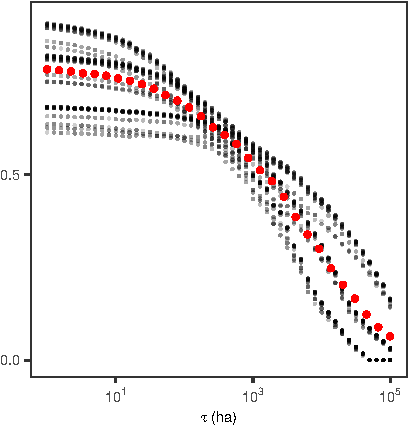
\includegraphics[keepaspectratio]{code_detectability_irrigated_areas_files/figure-latex/uasa_on_weights-6.pdf}}
\pandocbounded{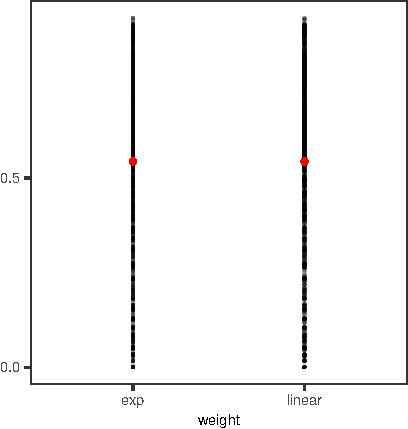
\includegraphics[keepaspectratio]{code_detectability_irrigated_areas_files/figure-latex/uasa_on_weights-7.pdf}}

\begin{Shaded}
\begin{Highlighting}[]
\CommentTok{\# MERGE UA/SA PLOTS \#\#\#\#\#\#\#\#\#\#\#\#\#\#\#\#\#\#\#\#\#\#\#\#\#\#\#\#\#\#\#\#\#\#\#\#\#\#\#\#\#\#\#\#\#\#\#\#\#\#\#\#\#\#\#\#\#\#\#\#}

\NormalTok{top }\OtherTok{\textless{}{-}} \FunctionTok{plot\_grid}\NormalTok{(plot\_uncertainty, plot\_agreement, plot\_indices3,}
                 \AttributeTok{ncol =} \DecValTok{3}\NormalTok{, }\AttributeTok{labels =} \StringTok{"auto"}\NormalTok{, }\AttributeTok{rel\_widths =} \FunctionTok{c}\NormalTok{(}\FloatTok{0.4}\NormalTok{, }\FloatTok{0.3}\NormalTok{, }\FloatTok{0.3}\NormalTok{))}
\end{Highlighting}
\end{Shaded}

\begin{verbatim}
## Warning in scale_x_log10(labels = label_log(digits = 2)): log-10 transformation introduced infinite values.
## log-10 transformation introduced infinite values.
## log-10 transformation introduced infinite values.
## log-10 transformation introduced infinite values.
\end{verbatim}

\begin{Shaded}
\begin{Highlighting}[]
\NormalTok{bottom }\OtherTok{\textless{}{-}} \FunctionTok{plot\_grid}\NormalTok{(a3, b3, c3, d3, }\AttributeTok{ncol =} \DecValTok{4}\NormalTok{, }\AttributeTok{rel\_widths =} \FunctionTok{c}\NormalTok{(}\FloatTok{0.35}\NormalTok{, }\FloatTok{0.25}\NormalTok{, }\FloatTok{0.2}\NormalTok{, }\FloatTok{0.2}\NormalTok{), }\AttributeTok{labels =} \StringTok{"d"}\NormalTok{)}
\end{Highlighting}
\end{Shaded}

\begin{verbatim}
## Warning in scale_x_log10(labels = label_log(digits = 2)): log-10 transformation introduced infinite values.
## log-10 transformation introduced infinite values.
\end{verbatim}

\begin{verbatim}
## Warning: Removed 157 rows containing non-finite outside the scale range
## (`stat_summary_bin()`).
\end{verbatim}

\begin{Shaded}
\begin{Highlighting}[]
\FunctionTok{plot\_grid}\NormalTok{(top, bottom, }\AttributeTok{ncol =} \DecValTok{1}\NormalTok{)}
\end{Highlighting}
\end{Shaded}

\pandocbounded{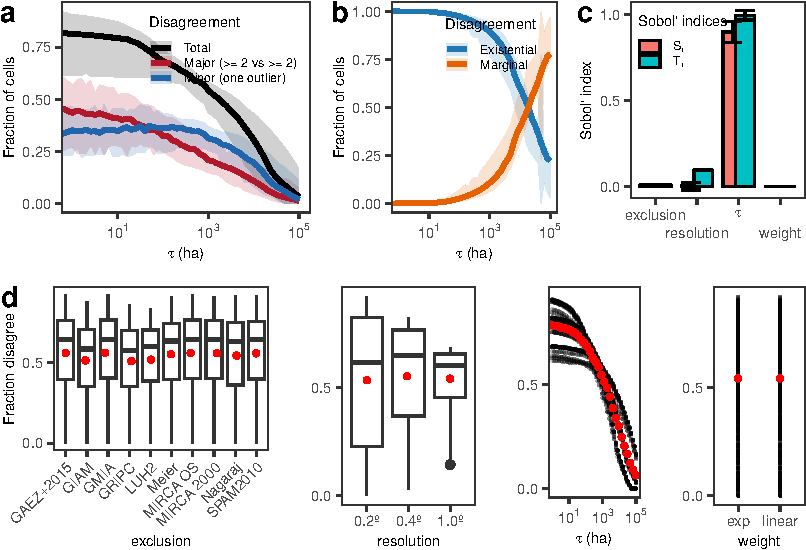
\includegraphics[keepaspectratio]{code_detectability_irrigated_areas_files/figure-latex/plot_weights-1.pdf}}

\newpage

\section{\texorpdfstring{The maximum threshold for existence
disagreement:
\(\tau_{\text{max}}\)}{The maximum threshold for existence disagreement: \textbackslash tau\_\{\textbackslash text\{max\}\}}}\label{the-maximum-threshold-for-existence-disagreement-tau_textmax}

\begin{Shaded}
\begin{Highlighting}[]
\CommentTok{\# COMPUTE TAU MAX \#\#\#\#\#\#\#\#\#\#\#\#\#\#\#\#\#\#\#\#\#\#\#\#\#\#\#\#\#\#\#\#\#\#\#\#\#\#\#\#\#\#\#\#\#\#\#\#\#\#\#\#\#\#\#\#\#\#\#\#\#\#}
\DocumentationTok{\#\#\#\#\#\#\#\#\#\#\#\#\#\#\#\#\#\#\#\#\#\#\#\#\#\#\#\#\#\#\#\#\#\#\#\#\#\#\#\#\#\#\#\#\#\#\#\#\#\#\#\#\#\#\#\#\#\#\#\#\#\#\#\#\#\#\#\#\#\#\#\#\#\#\#\#\#\#\#\#}

\CommentTok{\# Tau max is the largest irrigation threshold at which at least one dataset}
\CommentTok{\# classifies the cell as essentially unirrigated  while another classifies}
\CommentTok{\# it as irrigated. Tau max thus quantifies how large the ontological disagreement}
\CommentTok{\# on irrigation is. We also set NA to two cases:}

\CommentTok{\# {-} Universally non{-}irrigated cells: all datasets report areas \textless{}= threshold.}
\CommentTok{\# {-} Universally irrigated cells: all datasets report areas \textgreater{}threshold.}

\CommentTok{\# NA cells are cells for which there is agreement irrigation exists or it is absent.}

\DocumentationTok{\#\# Compute tau\_max\_results {-}{-}{-}{-}{-}{-}{-}{-}{-}{-}{-}{-}{-}{-}{-}{-}{-}{-}{-}{-}{-}{-}{-}{-}{-}{-}{-}{-}{-}{-}{-}{-}{-}{-}{-}{-}{-}{-}{-}{-}{-}{-}{-}{-}{-}{-}{-}{-}{-}{-}{-}{-}{-}}

\NormalTok{tau\_max\_results }\OtherTok{\textless{}{-}} \FunctionTok{rbindlist}\NormalTok{(}
\NormalTok{  parallel}\SpecialCharTok{::}\FunctionTok{mclapply}\NormalTok{(resolutions, }\ControlFlowTok{function}\NormalTok{(res) \{}

\NormalTok{    dt\_res\_long }\OtherTok{\textless{}{-}}\NormalTok{ dt[resolution }\SpecialCharTok{==}\NormalTok{ res]}

    \CommentTok{\# datasets present at this resolution}
\NormalTok{    ds\_res }\OtherTok{\textless{}{-}} \FunctionTok{sort}\NormalTok{(}\FunctionTok{unique}\NormalTok{(dt\_res\_long}\SpecialCharTok{$}\NormalTok{dataset))}

    \CommentTok{\# resolution{-}specific detectability thresholds (in ha){-}{-}{-}{-}{-}{-}{-}{-}{-}{-}{-}{-}{-}{-}{-}{-}{-}{-}{-}{-}{-}{-}}
    
\NormalTok{    zero\_tol\_ha }\OtherTok{\textless{}{-}} \ControlFlowTok{switch}\NormalTok{(res,}
      \StringTok{"0.2deg"} \OtherTok{=} \DecValTok{400}\NormalTok{, }\CommentTok{\# 1\% of cell at 0.2°}
      \StringTok{"0.4deg"} \OtherTok{=} \DecValTok{1600}\NormalTok{, }\CommentTok{\# 1\% of cell at 0.4°}
      \StringTok{"1deg"} \OtherTok{=} \DecValTok{10000}\NormalTok{, }\CommentTok{\# 1\% of cell at 1°}
      \FunctionTok{stop}\NormalTok{(}\StringTok{"Unknown resolution: "}\NormalTok{, res))}

    \FunctionTok{rbindlist}\NormalTok{(}
      \FunctionTok{lapply}\NormalTok{(dataset\_vec, }\ControlFlowTok{function}\NormalTok{(scn) \{}

        \CommentTok{\# which datasets to use {-}{-}{-}{-}{-}{-}{-}{-}{-}{-}{-}{-}{-}{-}{-}{-}{-}{-}{-}{-}{-}{-}{-}{-}{-}{-}{-}{-}{-}{-}{-}{-}{-}{-}{-}{-}{-}{-}{-}{-}{-}{-}{-}{-}{-}{-}{-}}
        
        \ControlFlowTok{if}\NormalTok{ (scn }\SpecialCharTok{==} \StringTok{"all"}\NormalTok{) \{}
\NormalTok{          use\_ds }\OtherTok{\textless{}{-}}\NormalTok{ ds\_res}
\NormalTok{        \} }\ControlFlowTok{else}\NormalTok{ \{}
\NormalTok{          use\_ds }\OtherTok{\textless{}{-}} \FunctionTok{setdiff}\NormalTok{(ds\_res, scn)}
\NormalTok{        \}}

        \CommentTok{\# if only one dataset left, skip {-}{-}{-}{-}{-}{-}{-}{-}{-}{-}{-}{-}{-}{-}{-}{-}{-}{-}{-}{-}{-}{-}{-}{-}{-}{-}{-}{-}{-}{-}{-}{-}{-}{-}{-}{-}{-}{-}}
        
        \ControlFlowTok{if}\NormalTok{ (}\FunctionTok{length}\NormalTok{(use\_ds) }\SpecialCharTok{\textless{}} \DecValTok{2}\DataTypeTok{L}\NormalTok{) }\FunctionTok{return}\NormalTok{(}\ConstantTok{NULL}\NormalTok{)}

        \CommentTok{\# reshape to wide {-}{-}{-}{-}{-}{-}{-}{-}{-}{-}{-}{-}{-}{-}{-}{-}{-}{-}{-}{-}{-}{-}{-}{-}{-}{-}{-}{-}{-}{-}{-}{-}{-}{-}{-}{-}{-}{-}{-}{-}{-}{-}{-}{-}{-}{-}{-}{-}{-}{-}{-}{-}}
        
        
\NormalTok{        dt\_res\_wide }\OtherTok{\textless{}{-}} \FunctionTok{dcast}\NormalTok{(}
\NormalTok{          dt\_res\_long[dataset }\SpecialCharTok{\%in\%}\NormalTok{ use\_ds],}
\NormalTok{          lon }\SpecialCharTok{+}\NormalTok{ lat }\SpecialCharTok{+}\NormalTok{ country }\SpecialCharTok{+}\NormalTok{ code }\SpecialCharTok{+}\NormalTok{ continent }\SpecialCharTok{\textasciitilde{}}\NormalTok{ dataset,}
          \AttributeTok{value.var =} \StringTok{"mha"}\NormalTok{, }\AttributeTok{fill =} \DecValTok{0}
\NormalTok{        )}

\NormalTok{        tau\_max\_dt }\OtherTok{\textless{}{-}}\NormalTok{ tau\_grid[,}
          \FunctionTok{compute\_tau\_max\_existential\_fun}\NormalTok{(dt\_res\_wide, use\_ds, tau\_mha, tau\_ha,}
                                          \AttributeTok{zero\_tol\_ha =}\NormalTok{ zero\_tol\_ha)}
\NormalTok{        ]}

\NormalTok{        tau\_max\_dt[, }\StringTok{\textasciigrave{}}\AttributeTok{:=}\StringTok{\textasciigrave{}}\NormalTok{(}\AttributeTok{resolution =}\NormalTok{ res, }\AttributeTok{scenario =}\NormalTok{ scn)]}

\NormalTok{        tau\_max\_dt}
\NormalTok{      \}),}
      \AttributeTok{use.names =} \ConstantTok{TRUE}\NormalTok{, }\AttributeTok{fill =} \ConstantTok{TRUE}
\NormalTok{    )}
\NormalTok{  \}, }\AttributeTok{mc.cores =}\NormalTok{ ncores),}
  \AttributeTok{use.names =} \ConstantTok{TRUE}\NormalTok{, }\AttributeTok{fill =} \ConstantTok{TRUE}
\NormalTok{)}


\CommentTok{\# Add the countries {-}{-}{-}{-}{-}{-}{-}{-}{-}{-}{-}{-}{-}{-}{-}{-}{-}{-}{-}{-}{-}{-}{-}{-}{-}{-}{-}{-}{-}{-}{-}{-}{-}{-}{-}{-}{-}{-}{-}{-}{-}{-}{-}{-}{-}{-}{-}{-}{-}{-}{-}{-}{-}{-}{-}{-}{-}{-}{-}{-}}

\NormalTok{chunk\_size }\OtherTok{\textless{}{-}} \DecValTok{500000}\DataTypeTok{L}
\NormalTok{idx }\OtherTok{\textless{}{-}} \FunctionTok{split}\NormalTok{(}\FunctionTok{seq\_len}\NormalTok{(}\FunctionTok{nrow}\NormalTok{(tau\_max\_results)),}
             \FunctionTok{ceiling}\NormalTok{(}\FunctionTok{seq\_len}\NormalTok{(}\FunctionTok{nrow}\NormalTok{(tau\_max\_results)) }\SpecialCharTok{/}\NormalTok{ chunk\_size))}

\NormalTok{tau\_max\_results[, country}\SpecialCharTok{:=} \ConstantTok{NA\_character\_}\NormalTok{]}
\ControlFlowTok{for}\NormalTok{ (i }\ControlFlowTok{in}\NormalTok{ idx) \{}
\NormalTok{  tau\_max\_results[i, country}\SpecialCharTok{:=} \FunctionTok{lonlat\_to\_country}\NormalTok{(lon, lat, countries\_sf)]}
\NormalTok{\}}

\CommentTok{\# Add the continents {-}{-}{-}{-}{-}{-}{-}{-}{-}{-}{-}{-}{-}{-}{-}{-}{-}{-}{-}{-}{-}{-}{-}{-}{-}{-}{-}{-}{-}{-}{-}{-}{-}{-}{-}{-}{-}{-}{-}{-}{-}{-}{-}{-}{-}{-}{-}{-}{-}{-}{-}{-}{-}{-}{-}{-}{-}{-}{-}}

\FunctionTok{country\_to\_continent}\NormalTok{(tau\_max\_results)}

\CommentTok{\# Retrieve the round with all datasets and exclude the rest {-}{-}{-}{-}{-}{-}{-}{-}{-}{-}{-}{-}{-}{-}{-}{-}{-}{-}{-}{-}}

\NormalTok{tau\_max\_all }\OtherTok{\textless{}{-}}\NormalTok{ tau\_max\_results[scenario }\SpecialCharTok{==} \StringTok{"all"}\NormalTok{]}
\end{Highlighting}
\end{Shaded}

\begin{Shaded}
\begin{Highlighting}[]
\CommentTok{\# DEFINE PLOTS TAU MAX \#\#\#\#\#\#\#\#\#\#\#\#\#\#\#\#\#\#\#\#\#\#\#\#\#\#\#\#\#\#\#\#\#\#\#\#\#\#\#\#\#\#\#\#\#\#\#\#\#\#\#\#\#\#\#\#\#}

\CommentTok{\# Bin the tau max results {-}{-}{-}{-}{-}{-}{-}{-}{-}{-}{-}{-}{-}{-}{-}{-}{-}{-}{-}{-}{-}{-}{-}{-}{-}{-}{-}{-}{-}{-}{-}{-}{-}{-}{-}{-}{-}{-}{-}{-}{-}{-}{-}{-}{-}{-}{-}{-}{-}{-}{-}{-}{-}{-}}

\NormalTok{tau\_max\_results[, det\_thresh}\SpecialCharTok{:=} \FunctionTok{fcase}\NormalTok{(}
\NormalTok{  resolution }\SpecialCharTok{==} \StringTok{"0.2deg"}\NormalTok{, }\DecValTok{400}\NormalTok{,}
\NormalTok{  resolution }\SpecialCharTok{==} \StringTok{"0.4deg"}\NormalTok{, }\DecValTok{1600}\NormalTok{,}
\NormalTok{  resolution }\SpecialCharTok{==} \StringTok{"1deg"}\NormalTok{, }\DecValTok{10000}\NormalTok{)]}

\NormalTok{tau\_max\_results[, tau\_bin}\SpecialCharTok{:=} \FunctionTok{fcase}\NormalTok{(}
  \FunctionTok{is.na}\NormalTok{(tau\_max\_ha), }\StringTok{"Agreement"}\NormalTok{,}
\NormalTok{  tau\_max\_ha }\SpecialCharTok{\textless{}=} \DecValTok{2} \SpecialCharTok{*}\NormalTok{ det\_thresh, }\StringTok{"Low disagreement"}\NormalTok{,}
\NormalTok{  tau\_max\_ha }\SpecialCharTok{\textless{}=} \DecValTok{5} \SpecialCharTok{*}\NormalTok{ det\_thresh, }\StringTok{"Moderate disagreement"}\NormalTok{,}
\NormalTok{  tau\_max\_ha }\SpecialCharTok{\textless{}=} \DecValTok{10} \SpecialCharTok{*}\NormalTok{ det\_thresh, }\StringTok{"High disagreement"}\NormalTok{,}
  \AttributeTok{default =} \StringTok{"Extreme disagreement"}
\NormalTok{)]}

\NormalTok{tau\_max\_results[, tau\_bin}\SpecialCharTok{:=} \FunctionTok{factor}\NormalTok{(tau\_bin,}\AttributeTok{levels =} \FunctionTok{c}\NormalTok{(}\StringTok{"Agreement"}\NormalTok{,}
                                                       \StringTok{"Low disagreement"}\NormalTok{,}
                                                       \StringTok{"Moderate disagreement"}\NormalTok{,}
                                                       \StringTok{"High disagreement"}\NormalTok{,}
                                                       \StringTok{"Extreme disagreement"}\NormalTok{),}
                                    \AttributeTok{ordered =} \ConstantTok{TRUE}\NormalTok{)]}

\CommentTok{\# Proportion of cells disagreeing at 1\% threshold{-}{-}{-}{-}{-}{-}{-}{-}{-}{-}{-}{-}{-}{-}{-}{-}{-}{-}{-}{-}{-}{-}{-}{-}{-}{-}{-}{-}{-}{-}{-}}

\NormalTok{tau\_max\_results[, .N, .(tau\_bin, resolution)] }\SpecialCharTok{\%\textgreater{}\%}
\NormalTok{  .[, fraction }\SpecialCharTok{:=}\NormalTok{ N }\SpecialCharTok{/} \FunctionTok{sum}\NormalTok{(N), by }\OtherTok{=}\NormalTok{ resolution] }\SpecialCharTok{\%\textgreater{}\%}
\NormalTok{  .[}\SpecialCharTok{!}\NormalTok{tau\_bin }\SpecialCharTok{==} \StringTok{"Agreement"}\NormalTok{, }\FunctionTok{sum}\NormalTok{(fraction), resolution]}
\end{Highlighting}
\end{Shaded}

\begin{verbatim}
##    resolution        V1
##        <char>     <num>
## 1:     0.2deg 0.5846558
## 2:     0.4deg 0.5084122
## 3:       1deg 0.4158812
\end{verbatim}

\begin{Shaded}
\begin{Highlighting}[]
\NormalTok{thresh\_df }\OtherTok{\textless{}{-}} \FunctionTok{unique}\NormalTok{(tau\_max\_results[}\SpecialCharTok{!}\FunctionTok{is.na}\NormalTok{(det\_thresh), .(resolution, det\_thresh)])}

\CommentTok{\# ANALYSIS OF DATA {-}{-}{-}{-}{-}{-}{-}{-}{-}{-}{-}{-}{-}{-}{-}{-}{-}{-}{-}{-}{-}{-}{-}{-}{-}{-}{-}{-}{-}{-}{-}{-}{-}{-}{-}{-}{-}{-}{-}{-}{-}{-}{-}{-}{-}{-}{-}{-}{-}{-}{-}{-}{-}{-}{-}{-}{-}{-}{-}{-}{-}}

\CommentTok{\# Fraction of high and extreme ontological disagreement}
\CommentTok{\# across resolutions in each continent {-}{-}{-}{-}{-}{-}{-}{-}{-}{-}{-}{-}{-}{-}{-}{-}{-}{-}{-}{-}{-}{-}{-}{-}{-}{-}{-}{-}{-}{-}{-}{-}{-}{-}{-}{-}{-}{-}{-}{-}{-}}

\NormalTok{dt\_all }\OtherTok{\textless{}{-}}\NormalTok{ tau\_max\_results[scenario }\SpecialCharTok{==} \StringTok{"all"}\NormalTok{]}
\NormalTok{dt\_all[, N\_total }\SpecialCharTok{:=}\NormalTok{ .N, by }\OtherTok{=}\NormalTok{ .(resolution, continent)]}
\NormalTok{frac\_by\_rcb }\OtherTok{\textless{}{-}}\NormalTok{ dt\_all[, .(}\AttributeTok{frac =}\NormalTok{ .N }\SpecialCharTok{/} \FunctionTok{unique}\NormalTok{(N\_total)), }
\NormalTok{                      .(resolution, continent, tau\_bin)]}

\NormalTok{frac\_by\_rcb[, .(}\AttributeTok{min =} \FunctionTok{min}\NormalTok{(frac), }\AttributeTok{max =} \FunctionTok{max}\NormalTok{(frac)), .(continent, tau\_bin)] }\SpecialCharTok{\%\textgreater{}\%}
\NormalTok{  .[tau\_bin }\SpecialCharTok{\%in\%} \FunctionTok{c}\NormalTok{(}\StringTok{"Extreme disagreement"}\NormalTok{, }\StringTok{"High disagreement"}\NormalTok{)] }\SpecialCharTok{\%\textgreater{}\%}
\NormalTok{  .[}\FunctionTok{order}\NormalTok{(}\SpecialCharTok{{-}}\NormalTok{min)] }\SpecialCharTok{\%\textgreater{}\%}
\NormalTok{  .[, .(}\AttributeTok{min =} \FunctionTok{min}\NormalTok{(min), }\AttributeTok{max =} \FunctionTok{max}\NormalTok{(max)), .(continent)]}
\end{Highlighting}
\end{Shaded}

\begin{verbatim}
##    continent        min       max
##       <char>      <num>     <num>
## 1:      Asia 0.16245713 0.4002044
## 2:   Oceania 0.11820160 0.2261484
## 3:    Europe 0.11685770 0.1918899
## 4:  Americas 0.08104375 0.1758854
## 5:    Africa 0.04364620 0.1096917
\end{verbatim}

\begin{Shaded}
\begin{Highlighting}[]
\CommentTok{\# distribution of detectability limits}

\NormalTok{tau\_max\_results[, .N, .(tau\_max\_ha, resolution, scenario)]}
\end{Highlighting}
\end{Shaded}

\begin{verbatim}
##      tau_max_ha resolution scenario     N
##           <num>     <char>   <char> <int>
##   1:         NA     0.2deg      all 50531
##   2:   1584.893     0.2deg      all  5914
##   3:   1000.000     0.2deg      all  2862
##   4:   5011.872     0.2deg      all  7216
##   5:   3981.072     0.2deg      all  5021
##  ---                                     
## 600:  31622.777       1deg     spam   275
## 601:  25118.864       1deg     spam   267
## 602:  63095.734       1deg     spam   260
## 603:  79432.823       1deg     spam   265
## 604: 100000.000       1deg     spam   694
\end{verbatim}

\begin{Shaded}
\begin{Highlighting}[]
\NormalTok{tmp }\OtherTok{\textless{}{-}} \FunctionTok{copy}\NormalTok{(tau\_max\_results)}
\NormalTok{tmp[}\FunctionTok{is.na}\NormalTok{(tau\_max\_ha), tau\_max\_ha}\SpecialCharTok{:=} \FloatTok{0.1}\NormalTok{]}

\NormalTok{plot\_ecdf }\OtherTok{\textless{}{-}} \FunctionTok{ggplot}\NormalTok{(tmp, }\FunctionTok{aes}\NormalTok{(}\AttributeTok{x =}\NormalTok{ tau\_max\_ha, }\AttributeTok{color =}\NormalTok{ resolution)) }\SpecialCharTok{+}
  \FunctionTok{stat\_ecdf}\NormalTok{(}\AttributeTok{size =} \DecValTok{1}\NormalTok{) }\SpecialCharTok{+}
  \FunctionTok{scale\_x\_log10}\NormalTok{(}\AttributeTok{labels =} \FunctionTok{label\_log}\NormalTok{(}\AttributeTok{digits =} \DecValTok{2}\NormalTok{)) }\SpecialCharTok{+}
  \FunctionTok{scale\_color\_manual}\NormalTok{(}\AttributeTok{values =}\NormalTok{ res\_palette) }\SpecialCharTok{+}
  \FunctionTok{labs}\NormalTok{(}\AttributeTok{x =} \FunctionTok{expression}\NormalTok{(tau[max]}\SpecialCharTok{\textasciitilde{}}\StringTok{"(ha)"}\NormalTok{), }\AttributeTok{y =} \StringTok{"Fraction grid cells"}\NormalTok{,}
       \AttributeTok{color =} \StringTok{"Resolution"}\NormalTok{) }\SpecialCharTok{+}
  \FunctionTok{theme\_AP}\NormalTok{() }\SpecialCharTok{+}
  \FunctionTok{theme}\NormalTok{(}\AttributeTok{legend.position =} \FunctionTok{c}\NormalTok{(}\FloatTok{0.65}\NormalTok{, }\FloatTok{0.25}\NormalTok{))}
\end{Highlighting}
\end{Shaded}

\begin{verbatim}
## Warning: Using `size` aesthetic for lines was deprecated in ggplot2 3.4.0.
## i Please use `linewidth` instead.
## This warning is displayed once per session.
## Call `lifecycle::last_lifecycle_warnings()` to see where this warning was
## generated.
\end{verbatim}

\begin{Shaded}
\begin{Highlighting}[]
\NormalTok{plot\_ecdf}
\end{Highlighting}
\end{Shaded}

\pandocbounded{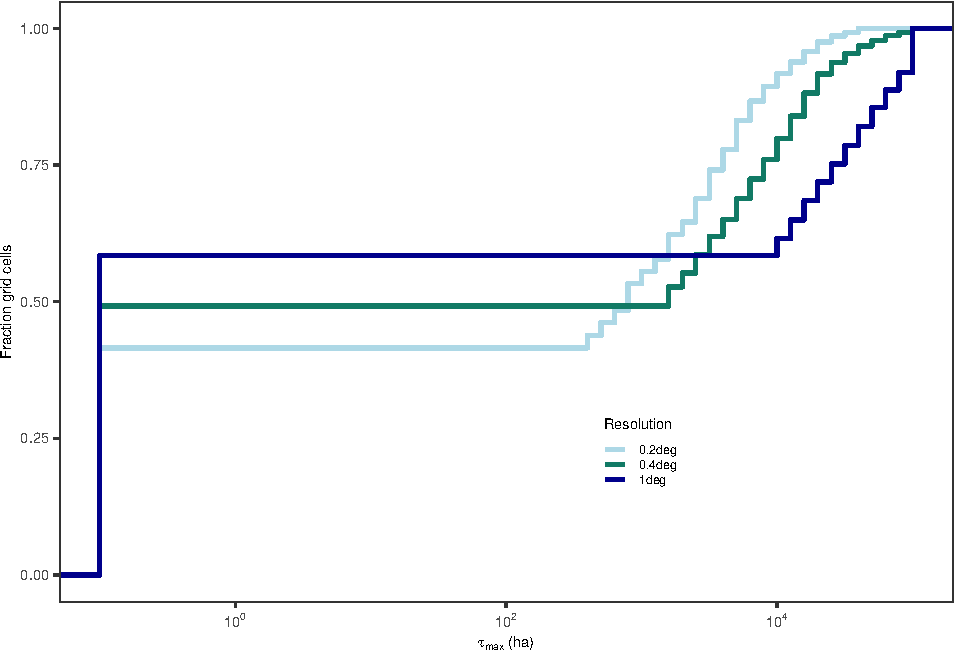
\includegraphics[keepaspectratio]{code_detectability_irrigated_areas_files/figure-latex/define_plots_taumax-1.pdf}}

\begin{Shaded}
\begin{Highlighting}[]
\CommentTok{\# How much of the world is perfectably detectable vs fundamentally ambiguous?}

\NormalTok{plot\_stacked }\OtherTok{\textless{}{-}}\NormalTok{ tau\_max\_results[, .N, by }\OtherTok{=}\NormalTok{ .(resolution, tau\_bin)] }\SpecialCharTok{\%\textgreater{}\%}
\NormalTok{  .[, frac }\SpecialCharTok{:=}\NormalTok{ N }\SpecialCharTok{/} \FunctionTok{sum}\NormalTok{(N), by }\OtherTok{=}\NormalTok{ resolution] }\SpecialCharTok{|\textgreater{}}
  \FunctionTok{ggplot}\NormalTok{(}\FunctionTok{aes}\NormalTok{(resolution, frac, }\AttributeTok{fill =}\NormalTok{ tau\_bin)) }\SpecialCharTok{+}
  \FunctionTok{geom\_col}\NormalTok{() }\SpecialCharTok{+}
  \FunctionTok{scale\_y\_continuous}\NormalTok{() }\SpecialCharTok{+}
  \FunctionTok{scale\_fill\_manual}\NormalTok{(}\AttributeTok{values =}\NormalTok{ tau\_palette, }\AttributeTok{name =} \FunctionTok{expression}\NormalTok{(tau[max])) }\SpecialCharTok{+}
  \FunctionTok{labs}\NormalTok{(}\AttributeTok{y =} \StringTok{"Fraction grid cells"}\NormalTok{, }\AttributeTok{x =} \ConstantTok{NULL}\NormalTok{, }\AttributeTok{fill =} \FunctionTok{expression}\NormalTok{(tau[max])) }\SpecialCharTok{+}
  \FunctionTok{theme\_AP}\NormalTok{() }\SpecialCharTok{+}
  \FunctionTok{theme}\NormalTok{(}\AttributeTok{legend.position =} \StringTok{"none"}\NormalTok{) }

\NormalTok{plot\_stacked}
\end{Highlighting}
\end{Shaded}

\pandocbounded{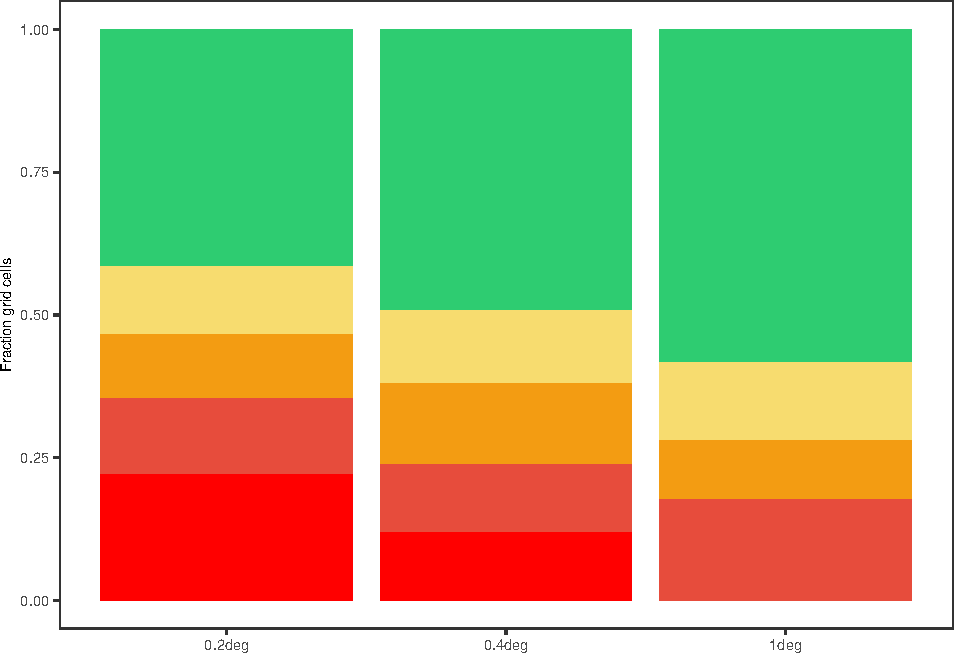
\includegraphics[keepaspectratio]{code_detectability_irrigated_areas_files/figure-latex/define_plots_taumax-2.pdf}}

\begin{Shaded}
\begin{Highlighting}[]
\CommentTok{\# Boxplots of tau max per resolution {-}{-}{-}{-}{-}{-}{-}{-}{-}{-}{-}{-}{-}{-}{-}{-}{-}{-}{-}{-}{-}{-}{-}{-}{-}{-}{-}{-}{-}{-}{-}{-}{-}{-}{-}{-}{-}{-}{-}{-}{-}{-}{-}}

\NormalTok{plot\_box }\OtherTok{\textless{}{-}} \FunctionTok{ggplot}\NormalTok{(tau\_max\_results[}\SpecialCharTok{!}\FunctionTok{is.na}\NormalTok{(tau\_max\_ha) }\SpecialCharTok{\&}\NormalTok{ tau\_max\_ha }\SpecialCharTok{\textgreater{}} \DecValTok{0}\NormalTok{],}
                   \FunctionTok{aes}\NormalTok{(resolution, tau\_max\_ha, }\AttributeTok{fill =}\NormalTok{ resolution)) }\SpecialCharTok{+}
  \FunctionTok{geom\_boxplot}\NormalTok{(}\AttributeTok{outlier.shape =} \ConstantTok{NA}\NormalTok{, }\AttributeTok{alpha =} \FloatTok{0.85}\NormalTok{) }\SpecialCharTok{+}
  \FunctionTok{geom\_hline}\NormalTok{(}\AttributeTok{data =}\NormalTok{ thresh\_df, }\FunctionTok{aes}\NormalTok{(}\AttributeTok{yintercept =}\NormalTok{ det\_thresh, }\AttributeTok{color =}\NormalTok{ resolution),}
             \AttributeTok{linetype =} \StringTok{"dashed"}\NormalTok{, }\AttributeTok{linewidth =} \FloatTok{0.7}\NormalTok{, }\AttributeTok{show.legend =} \ConstantTok{FALSE}\NormalTok{) }\SpecialCharTok{+}
  \FunctionTok{scale\_y\_log10}\NormalTok{(}\AttributeTok{labels =}\NormalTok{ scales}\SpecialCharTok{::}\FunctionTok{label\_log}\NormalTok{(}\AttributeTok{digits =} \DecValTok{2}\NormalTok{),}
                \AttributeTok{name   =} \FunctionTok{expression}\NormalTok{(tau[max]}\SpecialCharTok{\textasciitilde{}}\StringTok{"(ha)"}\NormalTok{)) }\SpecialCharTok{+}
  \FunctionTok{scale\_fill\_manual}\NormalTok{(}\AttributeTok{values =}\NormalTok{ res\_palette, }\AttributeTok{guide =} \StringTok{"none"}\NormalTok{) }\SpecialCharTok{+}
  \FunctionTok{scale\_color\_manual}\NormalTok{(}\AttributeTok{values =}\NormalTok{ res\_palette, }\AttributeTok{guide =} \StringTok{"none"}\NormalTok{) }\SpecialCharTok{+}
  \FunctionTok{labs}\NormalTok{(}
    \AttributeTok{x =} \ConstantTok{NULL}\NormalTok{,}
\NormalTok{  ) }\SpecialCharTok{+}
  \FunctionTok{theme\_AP}\NormalTok{() }\SpecialCharTok{+}
  \FunctionTok{theme}\NormalTok{()}

\NormalTok{plot\_box}
\end{Highlighting}
\end{Shaded}

\pandocbounded{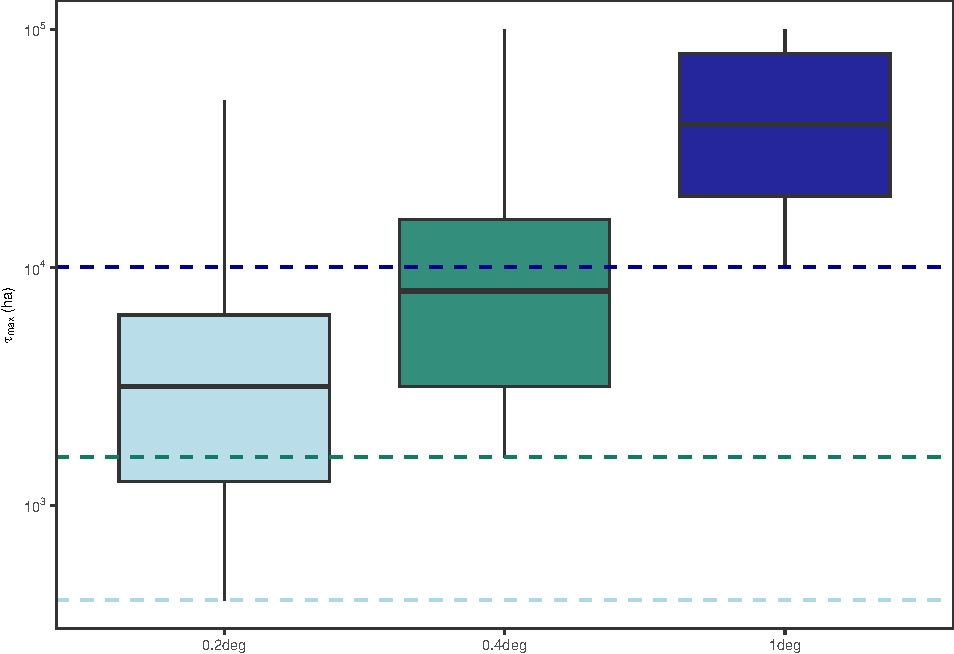
\includegraphics[keepaspectratio]{code_detectability_irrigated_areas_files/figure-latex/define_plots_taumax-3.pdf}}

\begin{Shaded}
\begin{Highlighting}[]
\CommentTok{\# MERGE TAU MAX PLOTS \#\#\#\#\#\#\#\#\#\#\#\#\#\#\#\#\#\#\#\#\#\#\#\#\#\#\#\#\#\#\#\#\#\#\#\#\#\#\#\#\#\#\#\#\#\#\#\#\#\#\#\#\#\#\#\#\#\#}

\NormalTok{top }\OtherTok{\textless{}{-}} \FunctionTok{plot\_grid}\NormalTok{(plot\_ecdf, plot\_stacked, plot\_box, }\AttributeTok{ncol =} \DecValTok{1}\NormalTok{,}
                 \AttributeTok{rel\_heights =} \FunctionTok{c}\NormalTok{(}\FloatTok{0.35}\NormalTok{, }\FloatTok{0.35}\NormalTok{, }\FloatTok{0.3}\NormalTok{),}
          \AttributeTok{labels =} \StringTok{"auto"}\NormalTok{)}

\NormalTok{top}
\end{Highlighting}
\end{Shaded}

\pandocbounded{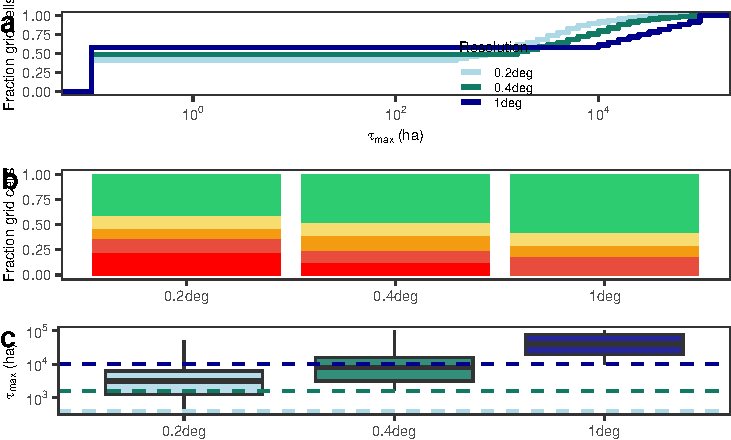
\includegraphics[keepaspectratio]{code_detectability_irrigated_areas_files/figure-latex/merge_tau_max-1.pdf}}

\begin{Shaded}
\begin{Highlighting}[]
\CommentTok{\# The map \#\#\#\#\#\#\#\#\#\#\#\#\#\#\#\#\#\#\#\#\#\#\#\#\#\#\#\#\#\#\#\#\#\#\#\#\#\#\#\#\#\#\#\#\#\#\#\#\#\#\#\#\#\#\#\#\#\#\#\#\#\#\#\#\#\#\#\#\#\#}

\NormalTok{plot\_raster }\OtherTok{\textless{}{-}} \FunctionTok{ggplot}\NormalTok{(tau\_max\_results, }\FunctionTok{aes}\NormalTok{(lon, lat, }\AttributeTok{fill =}\NormalTok{ tau\_bin)) }\SpecialCharTok{+}
  \FunctionTok{geom\_raster}\NormalTok{() }\SpecialCharTok{+}
  \FunctionTok{coord\_equal}\NormalTok{(}\AttributeTok{expand =} \ConstantTok{FALSE}\NormalTok{) }\SpecialCharTok{+}
  \FunctionTok{facet\_wrap}\NormalTok{(}\SpecialCharTok{\textasciitilde{}}\NormalTok{ resolution, }\AttributeTok{ncol =} \DecValTok{1}\NormalTok{) }\SpecialCharTok{+}
  \FunctionTok{scale\_fill\_manual}\NormalTok{(}\AttributeTok{values =}\NormalTok{ tau\_palette, }\AttributeTok{name =} \FunctionTok{expression}\NormalTok{(tau[max])) }\SpecialCharTok{+}
  \FunctionTok{scale\_x\_continuous}\NormalTok{(}\AttributeTok{expand =} \FunctionTok{c}\NormalTok{(}\DecValTok{0}\NormalTok{, }\DecValTok{0}\NormalTok{)) }\SpecialCharTok{+}
  \FunctionTok{scale\_y\_continuous}\NormalTok{(}\AttributeTok{expand =} \FunctionTok{c}\NormalTok{(}\DecValTok{0}\NormalTok{, }\DecValTok{0}\NormalTok{)) }\SpecialCharTok{+}
  \FunctionTok{theme\_AP}\NormalTok{() }\SpecialCharTok{+}
  \FunctionTok{theme}\NormalTok{(}\AttributeTok{panel.grid =} \FunctionTok{element\_blank}\NormalTok{(),}
        \AttributeTok{strip.text =} \FunctionTok{element\_text}\NormalTok{(}\AttributeTok{size =} \DecValTok{11}\NormalTok{),}
        \AttributeTok{legend.position =} \StringTok{"top"}\NormalTok{) }\SpecialCharTok{+}
  \FunctionTok{labs}\NormalTok{(}\AttributeTok{x =} \StringTok{"longitude"}\NormalTok{, }\AttributeTok{y =} \StringTok{"latitude"}\NormalTok{) }\SpecialCharTok{+}
  \FunctionTok{guides}\NormalTok{(}\AttributeTok{fill =} \FunctionTok{guide\_legend}\NormalTok{(}\AttributeTok{nrow =} \DecValTok{3}\NormalTok{, }\AttributeTok{byrow =} \ConstantTok{TRUE}\NormalTok{))}

\NormalTok{plot\_raster}
\end{Highlighting}
\end{Shaded}

\begin{verbatim}
## Warning: Raster pixels are placed at uneven horizontal intervals and will be shifted
## i Consider using `geom_tile()` instead.
## Raster pixels are placed at uneven horizontal intervals and will be shifted
## i Consider using `geom_tile()` instead.
\end{verbatim}

\pandocbounded{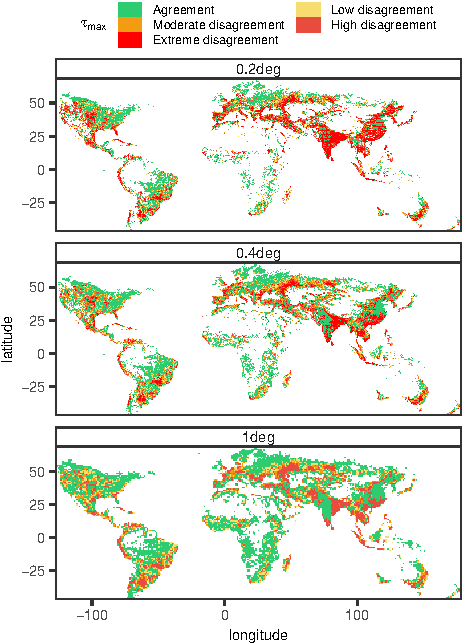
\includegraphics[keepaspectratio]{code_detectability_irrigated_areas_files/figure-latex/plot_map-1.pdf}}

\subsection{Composite figure}\label{composite-figure-1}

\begin{Shaded}
\begin{Highlighting}[]
\CommentTok{\# MERGE PLOTS \#\#\#\#\#\#\#\#\#\#\#\#\#\#\#\#\#\#\#\#\#\#\#\#\#\#\#\#\#\#\#\#\#\#\#\#\#\#\#\#\#\#\#\#\#\#\#\#\#\#\#\#\#\#\#\#\#\#\#\#\#\#\#\#\#\#}

\FunctionTok{plot\_grid}\NormalTok{(top, plot\_raster, }\AttributeTok{rel\_widths =} \FunctionTok{c}\NormalTok{(}\FloatTok{0.3}\NormalTok{, }\FloatTok{0.7}\NormalTok{), }\AttributeTok{ncol =} \DecValTok{2}\NormalTok{, }\AttributeTok{labels =} \FunctionTok{c}\NormalTok{(}\StringTok{""}\NormalTok{, }\StringTok{"d"}\NormalTok{))}
\end{Highlighting}
\end{Shaded}

\begin{verbatim}
## Warning: Raster pixels are placed at uneven horizontal intervals and will be shifted
## i Consider using `geom_tile()` instead.
## Raster pixels are placed at uneven horizontal intervals and will be shifted
## i Consider using `geom_tile()` instead.
\end{verbatim}

\pandocbounded{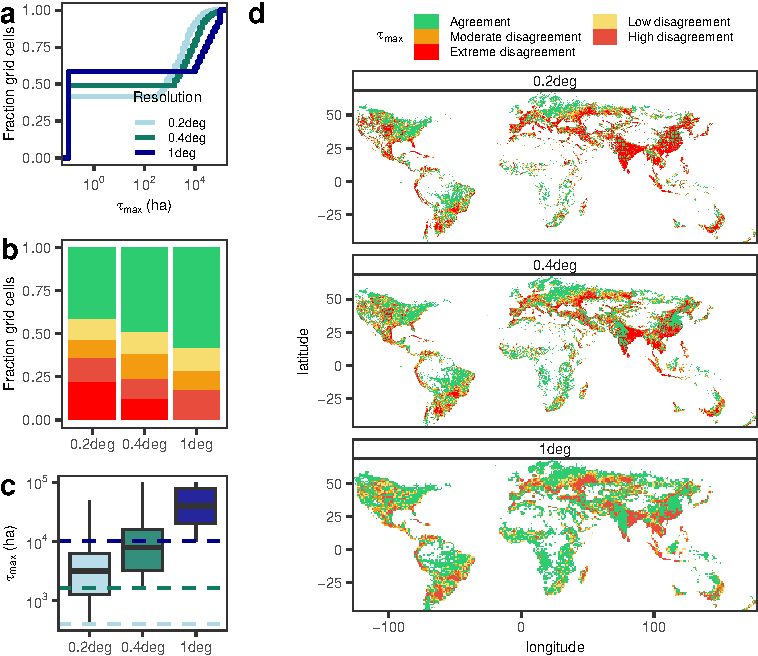
\includegraphics[keepaspectratio]{code_detectability_irrigated_areas_files/figure-latex/merge_plot_tau_max_map-1.pdf}}

\subsubsection{Which datasets drive deep
disagreement?}\label{which-datasets-drive-deep-disagreement}

\begin{Shaded}
\begin{Highlighting}[]
\CommentTok{\# WHICH DATASETS DRIVE DEEP DISAGREEMENT? {-}{-}{-}{-}{-}{-}{-}{-}{-}{-}{-}{-}{-}{-}{-}{-}{-}{-}{-}{-}{-}{-}{-}{-}{-}{-}{-}{-}{-}{-}{-}{-}{-}{-}{-}{-}{-}{-}}

\CommentTok{\# Check leave one{-}out scenarios {-}{-}{-}{-}{-}{-}{-}{-}{-}{-}{-}{-}{-}{-}{-}{-}{-}{-}{-}{-}{-}{-}{-}{-}{-}{-}{-}{-}{-}{-}{-}{-}{-}{-}{-}{-}{-}{-}{-}{-}{-}{-}{-}{-}{-}{-}{-}{-}}

\NormalTok{loo\_stats }\OtherTok{\textless{}{-}}\NormalTok{ tau\_max\_results[resolution }\SpecialCharTok{==} \StringTok{"0.2deg"}\NormalTok{,}
\NormalTok{                             .(}\AttributeTok{median\_tau =} \FunctionTok{median}\NormalTok{(tau\_max\_ha, }\AttributeTok{na.rm =} \ConstantTok{TRUE}\NormalTok{)),}
\NormalTok{                             scenario] }\SpecialCharTok{\%\textgreater{}\%}
\NormalTok{  .[}\FunctionTok{order}\NormalTok{(}\SpecialCharTok{{-}}\NormalTok{median\_tau)]}

\NormalTok{loo\_stats}
\end{Highlighting}
\end{Shaded}

\begin{verbatim}
##      scenario median_tau
##        <char>      <num>
##  1:       all   3162.278
##  2:   gaez_v4   3162.278
##  3:      giam   3162.278
##  4:      gmia   3162.278
##  5:     gripc   3162.278
##  6:     meier   3162.278
##  7: mirca2000   3162.278
##  8:  mirca_os   3162.278
##  9:      spam   3162.278
## 10:      luh2   2511.886
## 11:   nagaraj   2511.886
\end{verbatim}

\begin{Shaded}
\begin{Highlighting}[]
\CommentTok{\# Most datasets do not drive median existential disagreement, but three datasets}
\CommentTok{\# reduce the median diagreement when removed: GIAM, LUH2, Nagaraj (c. 20\% reduction)}
\CommentTok{\# . They are the ones contributing most disagreement to existential contradictions}
\CommentTok{\# at the global median level (they most often say "there is irrigation" while}
\CommentTok{\# others say "there is no irrigation" or the other way around). So disagreement}
\CommentTok{\# is systemic but three datasets aplify it further.}

\CommentTok{\# Full stats {-}{-}{-}{-}{-}{-}{-}{-}{-}{-}{-}{-}{-}{-}{-}{-}{-}{-}{-}{-}{-}{-}{-}{-}{-}{-}{-}{-}{-}{-}{-}{-}{-}{-}{-}{-}{-}{-}{-}{-}{-}{-}{-}{-}{-}{-}{-}{-}{-}{-}{-}{-}{-}{-}{-}{-}{-}{-}{-}{-}{-}{-}{-}{-}{-}{-}{-}}

\NormalTok{loo\_stats\_full }\OtherTok{\textless{}{-}}\NormalTok{ tau\_max\_results[, .(}
    \AttributeTok{median\_tau =} \FunctionTok{median}\NormalTok{(tau\_max\_ha, }\AttributeTok{na.rm =} \ConstantTok{TRUE}\NormalTok{),}
    \AttributeTok{p75\_tau =} \FunctionTok{quantile}\NormalTok{(tau\_max\_ha, }\FloatTok{0.75}\NormalTok{, }\AttributeTok{na.rm =} \ConstantTok{TRUE}\NormalTok{),}
    \AttributeTok{p90\_tau =} \FunctionTok{quantile}\NormalTok{(tau\_max\_ha, }\FloatTok{0.90}\NormalTok{, }\AttributeTok{na.rm =} \ConstantTok{TRUE}\NormalTok{),}
    \AttributeTok{share\_gt\_1000 =} \FunctionTok{mean}\NormalTok{(tau\_max\_ha }\SpecialCharTok{\textgreater{}=} \DecValTok{1000}\NormalTok{, }\AttributeTok{na.rm =} \ConstantTok{TRUE}\NormalTok{)),}
\NormalTok{    scenario] }\SpecialCharTok{\%\textgreater{}\%}
\NormalTok{  .[}\FunctionTok{order}\NormalTok{(}\SpecialCharTok{{-}}\NormalTok{p90\_tau)]}

\NormalTok{loo\_stats\_full}
\end{Highlighting}
\end{Shaded}

\begin{verbatim}
##      scenario median_tau   p75_tau  p90_tau share_gt_1000
##        <char>      <num>     <num>    <num>         <num>
##  1:       all   3981.072 10000.000 19952.62     0.8514329
##  2:   gaez_v4   3981.072 10000.000 19952.62     0.8515995
##  3:      giam   3981.072  7943.282 19952.62     0.8361615
##  4:      gmia   3981.072 10000.000 19952.62     0.8514923
##  5:      luh2   3162.278  7943.282 19952.62     0.8357658
##  6:     meier   3981.072 10000.000 19952.62     0.8513763
##  7: mirca2000   3981.072 10000.000 19952.62     0.8543302
##  8:  mirca_os   3981.072 10000.000 19952.62     0.8527230
##  9:   nagaraj   3981.072 10000.000 19952.62     0.8316074
## 10:      spam   3981.072 10000.000 19952.62     0.8513446
## 11:     gripc   3981.072  7943.282 15848.93     0.8400983
\end{verbatim}

\begin{Shaded}
\begin{Highlighting}[]
\CommentTok{\# In half of all grid cells worldwide, at least one dataset reports \textgreater{}=1000 ha}
\CommentTok{\# of irrigation while another reports none. Removing most datasets does not}
\CommentTok{\# change anything. Removing GIAM, Nagaraj and LUH2 drops the median disagreement}
\CommentTok{\# and the extreme values, as they particularly increase existential contradictions}
\CommentTok{\# in the upper half of the distribution.}

\CommentTok{\# In which regions is each dataset structurally responsible for}
\CommentTok{\# deep existential contradictions? {-}{-}{-}{-}{-}{-}{-}{-}{-}{-}{-}{-}{-}{-}{-}{-}{-}{-}{-}{-}{-}{-}{-}{-}{-}{-}{-}{-}{-}{-}{-}{-}{-}{-}{-}{-}{-}{-}{-}{-}{-}{-}{-}{-}{-}{-}{-}}

\CommentTok{\# Compute spatial delta {-}{-}{-}{-}{-}{-}{-}{-}{-}{-}{-}}

\NormalTok{tau\_all }\OtherTok{\textless{}{-}}\NormalTok{ tau\_max\_results[scenario }\SpecialCharTok{==} \StringTok{"all"}\NormalTok{,.(lon, lat, resolution,}
                                               \AttributeTok{tau\_all =}\NormalTok{ tau\_max\_ha)]}

\CommentTok{\# Keep only datasets of interest{-}{-}}

\NormalTok{tau\_loo }\OtherTok{\textless{}{-}}\NormalTok{ tau\_max\_results[scenario }\SpecialCharTok{\%in\%} \FunctionTok{c}\NormalTok{(}\StringTok{"giam"}\NormalTok{, }\StringTok{"luh2"}\NormalTok{, }\StringTok{"nagaraj"}\NormalTok{),}
\NormalTok{                           .(lon, lat, country, continent, resolution, scenario,}
                             \AttributeTok{tau\_loo =}\NormalTok{ tau\_max\_ha)]}

\CommentTok{\# Merge {-}{-}{-}{-}{-}{-}{-}{-}{-}{-}{-}{-}{-}{-}{-}{-}{-}{-}{-}{-}{-}{-}{-}{-}{-}{-}{-}}

\NormalTok{tau\_delta }\OtherTok{\textless{}{-}} \FunctionTok{merge}\NormalTok{(tau\_loo, tau\_all, }\AttributeTok{by =} \FunctionTok{c}\NormalTok{(}\StringTok{"lon"}\NormalTok{, }\StringTok{"lat"}\NormalTok{, }\StringTok{"resolution"}\NormalTok{),}
                   \AttributeTok{all.x =} \ConstantTok{TRUE}\NormalTok{)}

\CommentTok{\# Compute difference {-}{-}{-}{-}{-}{-}{-}{-}{-}{-}{-}{-}{-}{-}}

\NormalTok{tau\_delta[, delta}\SpecialCharTok{:=}\NormalTok{ tau\_all }\SpecialCharTok{{-}}\NormalTok{ tau\_loo]}

\CommentTok{\# Let us define "strong amplification" of differences {-}{-}{-}{-}{-}{-}{-}{-}{-}{-}{-}{-}{-}{-}{-}{-}{-}{-}{-}{-}{-}{-}{-}{-}{-}{-}}
\CommentTok{\# Differences larger than 1000 ha.}

\NormalTok{tau\_delta[, strong}\SpecialCharTok{:=}\NormalTok{ delta }\SpecialCharTok{\textgreater{}=} \DecValTok{1000}\NormalTok{]}

\CommentTok{\# Compute overlap {-}{-}{-}{-}{-}{-}{-}{-}{-}{-}{-}{-}{-}{-}{-}{-}{-}{-}{-}{-}{-}{-}{-}{-}{-}{-}{-}{-}{-}{-}{-}{-}{-}{-}{-}{-}{-}{-}{-}{-}{-}{-}{-}{-}{-}{-}{-}{-}{-}{-}{-}{-}{-}{-}{-}{-}{-}{-}{-}{-}{-}{-}}

\NormalTok{influence\_matrix }\OtherTok{\textless{}{-}} \FunctionTok{dcast}\NormalTok{(tau\_delta[resolution }\SpecialCharTok{==} \StringTok{"0.2deg"}\NormalTok{],}
\NormalTok{                          lon }\SpecialCharTok{+}\NormalTok{ lat }\SpecialCharTok{\textasciitilde{}}\NormalTok{ scenario, }\AttributeTok{value.var =} \StringTok{"strong"}\NormalTok{,}
                          \AttributeTok{fill =} \ConstantTok{FALSE}\NormalTok{)}

\NormalTok{influence\_matrix[, n\_datasets}\SpecialCharTok{:=} \FunctionTok{rowSums}\NormalTok{(.SD), .SDcols }\OtherTok{=} \FunctionTok{c}\NormalTok{(}\StringTok{"giam"}\NormalTok{, }\StringTok{"luh2"}\NormalTok{, }\StringTok{"nagaraj"}\NormalTok{)]}

\FunctionTok{table}\NormalTok{(influence\_matrix}\SpecialCharTok{$}\NormalTok{n\_datasets)}
\end{Highlighting}
\end{Shaded}

\begin{verbatim}
## 
##     0     1 
## 38956 19073
\end{verbatim}

\begin{Shaded}
\begin{Highlighting}[]
\CommentTok{\# 0: deep disagreement in the cell not driven by these three.}
\CommentTok{\# 1: dataset{-}specific amplification.}
\CommentTok{\# 2: partial overlap.}
\CommentTok{\# 3: same hotspot amplified by all three.}

\CommentTok{\# Since there are zero cells where two datasets simultaneously aplify deep}
\CommentTok{\# disagreement (\textgreater{} 1000 ha) or all three do, it means that their influence is}
\CommentTok{\# spatially distinct. 22,615 cells show strong amplification but always due}
\CommentTok{\# to exactly one dataset.}

\CommentTok{\# Where does amplification concentrate? {-}{-}{-}{-}{-}{-}{-}{-}{-}{-}{-}{-}{-}{-}{-}{-}{-}{-}{-}{-}{-}{-}{-}{-}{-}{-}{-}{-}{-}{-}{-}{-}{-}{-}{-}{-}{-}{-}{-}{-}}

\NormalTok{regional\_amp }\OtherTok{\textless{}{-}}\NormalTok{ tau\_delta[resolution }\SpecialCharTok{==} \StringTok{"0.2deg"}\NormalTok{,}
\NormalTok{                          .(}\AttributeTok{median\_delta =} \FunctionTok{median}\NormalTok{(delta, }\AttributeTok{na.rm =} \ConstantTok{TRUE}\NormalTok{),}
                            \AttributeTok{share\_strong =} \FunctionTok{mean}\NormalTok{(delta }\SpecialCharTok{\textgreater{}=} \DecValTok{1000}\NormalTok{, }\AttributeTok{na.rm =} \ConstantTok{TRUE}\NormalTok{)),}
\NormalTok{                          .(continent, scenario)] }\SpecialCharTok{\%\textgreater{}\%}
\NormalTok{  .[}\FunctionTok{order}\NormalTok{(}\SpecialCharTok{{-}}\NormalTok{median\_delta)]}


\NormalTok{regional\_amp}
\end{Highlighting}
\end{Shaded}

\begin{verbatim}
##     continent scenario median_delta share_strong
##        <char>   <char>        <num>        <num>
##  1:  Americas     giam            0   0.06121637
##  2:  Americas     luh2            0   0.04826105
##  3:  Americas  nagaraj            0   0.14772132
##  4:    Europe     giam            0   0.16482642
##  5:    Europe     luh2            0   0.01957393
##  6:    Europe  nagaraj            0   0.14093907
##  7:    Africa     giam            0   0.02871651
##  8:    Africa     luh2            0   0.06763612
##  9:    Africa  nagaraj            0   0.04555172
## 10:      Asia     giam            0   0.12602012
## 11:      Asia     luh2            0   0.08506436
## 12:      Asia  nagaraj            0   0.13709471
## 13:   Oceania     giam            0   0.18408602
## 14:   Oceania     luh2            0   0.01701524
## 15:   Oceania  nagaraj            0   0.04653604
\end{verbatim}

\begin{Shaded}
\begin{Highlighting}[]
\CommentTok{\# Table shows which continents each dataset most strongly affects:}
\CommentTok{\# {-} Europe: GIAM dominates existential disagreement in Europe, LUH2 barely affects it.}
\CommentTok{\# {-} Asia: all three datasets contribute, LUH2 contributes less existential disagreement}
\CommentTok{\# {-} Ocenia: GIAM contributes the largest existential disagreement.}
\CommentTok{\# {-} Americas: Nagaraj.}
\CommentTok{\# {-} Africa: Overall amplification much lower, all contribute equally.}
\CommentTok{\# So overall there is no global problem dataset! And since they all show}
\CommentTok{\# median delta of zero everywhere, these datasets do not globally modify the}
\CommentTok{\# disagreement but create region{-}specific deep contradictions.}

\FunctionTok{ggplot}\NormalTok{(regional\_amp, }\FunctionTok{aes}\NormalTok{(scenario, share\_strong)) }\SpecialCharTok{+}
  \FunctionTok{geom\_bar}\NormalTok{(}\AttributeTok{stat =} \StringTok{"identity"}\NormalTok{) }\SpecialCharTok{+}
  \FunctionTok{coord\_flip}\NormalTok{() }\SpecialCharTok{+}
  \FunctionTok{facet\_wrap}\NormalTok{(}\SpecialCharTok{\textasciitilde{}}\NormalTok{continent, }\AttributeTok{ncol =} \DecValTok{5}\NormalTok{) }\SpecialCharTok{+}
  \FunctionTok{scale\_y\_continuous}\NormalTok{(}\AttributeTok{breaks =} \FunctionTok{breaks\_pretty}\NormalTok{(}\AttributeTok{n =} \DecValTok{2}\NormalTok{)) }\SpecialCharTok{+}
  \FunctionTok{theme\_AP}\NormalTok{() }\SpecialCharTok{+}
  \FunctionTok{labs}\NormalTok{(}\AttributeTok{x =} \StringTok{""}\NormalTok{, }\AttributeTok{y =} \StringTok{"Fraction cells"}\NormalTok{)}
\end{Highlighting}
\end{Shaded}

\pandocbounded{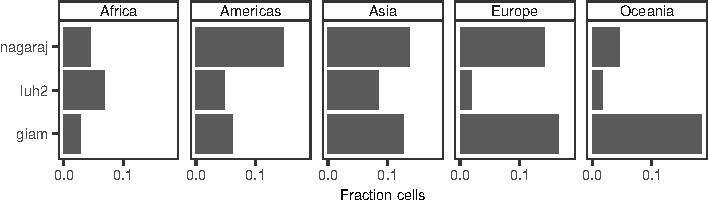
\includegraphics[keepaspectratio]{code_detectability_irrigated_areas_files/figure-latex/datasets_tau_max-1.pdf}}

\begin{Shaded}
\begin{Highlighting}[]
\CommentTok{\# Which dataset drives the 22,615 cells? {-}{-}{-}{-}{-}{-}{-}{-}{-}{-}{-}{-}{-}{-}{-}{-}{-}{-}{-}{-}{-}{-}{-}{-}{-}{-}{-}{-}{-}{-}{-}{-}{-}{-}{-}{-}{-}{-}{-}}

\NormalTok{influence\_matrix[, dominant }\SpecialCharTok{:=} \FunctionTok{fifelse}\NormalTok{(giam, }\StringTok{"GIAM"}\NormalTok{,}
                                       \FunctionTok{fifelse}\NormalTok{(luh2, }\StringTok{"LUH2"}\NormalTok{,}
                                               \FunctionTok{fifelse}\NormalTok{(nagaraj, }\StringTok{"Nagaraj"}\NormalTok{,}
                                                       \ConstantTok{NA\_character\_}\NormalTok{)))]}

\FunctionTok{table}\NormalTok{(influence\_matrix}\SpecialCharTok{$}\NormalTok{dominant)}
\end{Highlighting}
\end{Shaded}

\begin{verbatim}
## 
##    GIAM    LUH2 Nagaraj 
##    7325    3756    9117
\end{verbatim}

\subsection{How many grid cells
disagree?}\label{how-many-grid-cells-disagree}

\begin{Shaded}
\begin{Highlighting}[]
\CommentTok{\# DETECTABILITY OF IRRIGATED AREA ACROSS MAPS \#\#\#\#\#\#\#\#\#\#\#\#\#\#\#\#\#\#\#\#\#\#\#\#\#\#\#\#\#\#\#\#\#\#}
\DocumentationTok{\#\#\#\#\#\#\#\#\#\#\#\#\#\#\#\#\#\#\#\#\#\#\#\#\#\#\#\#\#\#\#\#\#\#\#\#\#\#\#\#\#\#\#\#\#\#\#\#\#\#\#\#\#\#\#\#\#\#\#\#\#\#\#\#\#\#\#\#\#\#\#\#\#\#\#\#\#\#\#\#}

\CommentTok{\# UNWEIGHTED: ALL CELLS COUNT EQUALLY \#\#\#\#\#\#\#\#\#\#\#\#\#\#\#\#\#\#\#\#\#\#\#\#\#\#\#\#\#\#\#\#\#\#\#\#\#\#\#\#\#\#}
\CommentTok{\# QUESTION ANSWERED: HOW MANY GRID CELLS DISAGREE? {-}{-}{-}{-}{-}{-}{-}{-}{-}{-}{-}{-}{-}{-}{-}{-}{-}{-}{-}{-}{-}{-}{-}{-}{-}{-}{-}{-}{-}}

\CommentTok{\# Make dataset wide and retrieve only the 0.2deg resolution one {-}{-}{-}{-}{-}{-}{-}{-}{-}{-}{-}{-}{-}{-}{-}{-}}

\NormalTok{dt\_wide }\OtherTok{\textless{}{-}}\NormalTok{ dt[resolution }\SpecialCharTok{==} \StringTok{"0.2deg"}\NormalTok{] }\SpecialCharTok{\%\textgreater{}\%}
  \FunctionTok{dcast}\NormalTok{(., lon }\SpecialCharTok{+}\NormalTok{ lat }\SpecialCharTok{+}\NormalTok{ country }\SpecialCharTok{+}\NormalTok{ code }\SpecialCharTok{+}\NormalTok{ continent }\SpecialCharTok{\textasciitilde{}}\NormalTok{ dataset, }\AttributeTok{value.var =} \StringTok{"mha"}\NormalTok{)}

\CommentTok{\# Retrieve 0.2deg resolution from tau max dataset and remove unwanted cols {-}{-}{-}{-}{-}}

\NormalTok{tau\_max\_results\_clean }\OtherTok{\textless{}{-}}\NormalTok{ tau\_max\_results[resolution }\SpecialCharTok{==} \StringTok{"0.2deg"} \SpecialCharTok{\&}\NormalTok{ scenario }\SpecialCharTok{==} \StringTok{"all"}\NormalTok{]}
\NormalTok{tau\_max\_results\_clean[, resolution}\SpecialCharTok{:=} \ConstantTok{NULL}\NormalTok{]}
\NormalTok{tau\_max\_results\_clean[, scenario}\SpecialCharTok{:=} \ConstantTok{NULL}\NormalTok{]}

\CommentTok{\# Merge {-}{-}{-}{-}{-}{-}{-}{-}{-}{-}{-}{-}{-}{-}{-}{-}{-}{-}{-}{-}{-}{-}{-}{-}{-}{-}{-}{-}{-}{-}{-}{-}{-}{-}{-}{-}{-}{-}{-}{-}{-}{-}{-}{-}{-}{-}{-}{-}{-}{-}{-}{-}{-}{-}{-}{-}{-}{-}{-}{-}{-}{-}{-}{-}{-}{-}{-}{-}{-}{-}{-}{-}}

\NormalTok{dt2 }\OtherTok{\textless{}{-}} \FunctionTok{merge}\NormalTok{(dt\_wide, tau\_max\_results\_clean[, .(lon, lat, tau\_max\_mha)],}
             \AttributeTok{by =} \FunctionTok{c}\NormalTok{(}\StringTok{"lon"}\NormalTok{, }\StringTok{"lat"}\NormalTok{), }\AttributeTok{all.x =} \ConstantTok{TRUE}\NormalTok{)}

\FunctionTok{setnames}\NormalTok{(dt2, dataset\_names, new\_dataset\_names)}

\CommentTok{\# Convert to ha for easier interpretation {-}{-}{-}{-}{-}{-}{-}{-}{-}{-}{-}{-}{-}{-}{-}{-}{-}{-}{-}{-}{-}{-}{-}{-}{-}{-}{-}{-}{-}{-}{-}{-}{-}{-}{-}{-}{-}{-}}

\NormalTok{dt2[, tau\_max\_ha}\SpecialCharTok{:=}\NormalTok{ tau\_max\_mha }\SpecialCharTok{*} \FloatTok{1e6}\NormalTok{]}

\CommentTok{\# Which percentage of the world is in disagreement on whether there is}
\CommentTok{\# or there is not irrigation? {-}{-}{-}{-}{-}{-}{-}{-}{-}{-}{-}{-}{-}{-}{-}{-}{-}{-}{-}{-}{-}{-}{-}{-}{-}{-}{-}{-}{-}{-}{-}{-}{-}{-}{-}{-}{-}{-}{-}{-}{-}{-}{-}{-}{-}{-}{-}{-}{-}{-}}

\NormalTok{frac\_cells\_nonid }\OtherTok{\textless{}{-}}\NormalTok{ dt2[, }\FunctionTok{mean}\NormalTok{(}\SpecialCharTok{!}\FunctionTok{is.na}\NormalTok{(tau\_max\_mha))]}
\NormalTok{frac\_cells\_nonid}
\end{Highlighting}
\end{Shaded}

\begin{verbatim}
## [1] 0.6072517
\end{verbatim}

\begin{Shaded}
\begin{Highlighting}[]
\FunctionTok{summary}\NormalTok{(dt2}\SpecialCharTok{$}\NormalTok{tau\_max\_ha)}
\end{Highlighting}
\end{Shaded}

\begin{verbatim}
##    Min. 1st Qu.  Median    Mean 3rd Qu.    Max.    NA's 
##   398.1  1258.9  3162.3  5871.8  6309.6 50118.7   50531
\end{verbatim}

\begin{Shaded}
\begin{Highlighting}[]
\CommentTok{\# Minimum = 398 ha, the detectability threshold for 0.2. No disagreement below it.}
\CommentTok{\#}
\CommentTok{\# Median disagreement (50\%) is eight times the detectability threshold (400 ha)}
\CommentTok{\# 75\% of disagreeing cells exceed 2.5x detectability.}
\CommentTok{\# Half exceed 8x detectability}

\CommentTok{\# Even after imposing a conservative 1\% rule some cells show contradictions at}
\CommentTok{\# tens of thousands of hectares; these are large irrigation landscapes, not}
\CommentTok{\# fragmented patches.}

\CommentTok{\# Existential contradictions occur at scales that are agronomically and}
\CommentTok{\# hydrologically meaningful and they are not confined to marginal lands. Include}
\CommentTok{\# cells where irrigation is either extensive or completely absent depending on}
\CommentTok{\# the dataset.Ddisagreement is not about "how much" irrigation exists but about}
\CommentTok{\# whether large irrigation systems exist at all in certain locations.}
\end{Highlighting}
\end{Shaded}

\subsection{How much irrigated land lies in
disagreeement?}\label{how-much-irrigated-land-lies-in-disagreeement}

\begin{Shaded}
\begin{Highlighting}[]
\CommentTok{\# WEIGHTED: CELLS WITH LARGER IRRIGATION COUNT MORE \#\#\#\#\#\#\#\#\#\#\#\#\#\#\#\#\#\#\#\#\#\#\#\#\#\#\#\#}
\CommentTok{\# QUESTION: HOW MUCH IRRIGATED LAND LIES IN DISAGREEMENT? {-}{-}{-}{-}{-}{-}{-}{-}{-}{-}{-}{-}{-}{-}{-}{-}{-}{-}{-}{-}{-}{-}}

\CommentTok{\# Keep only cells with existential disagreement {-}{-}{-}{-}{-}{-}{-}{-}{-}{-}{-}{-}{-}{-}{-}{-}{-}{-}{-}{-}{-}{-}{-}{-}{-}{-}{-}{-}{-}{-}{-}}
\CommentTok{\# (tau\_max\_ha non{-}NA)}

\NormalTok{dt2\_disagree }\OtherTok{\textless{}{-}}\NormalTok{ dt2[}\SpecialCharTok{!}\FunctionTok{is.na}\NormalTok{(tau\_max\_ha)]}

\CommentTok{\# Sanity check: no NA tau\_max\_ha left}
\FunctionTok{summary}\NormalTok{(dt2\_disagree}\SpecialCharTok{$}\NormalTok{tau\_max\_ha)}
\end{Highlighting}
\end{Shaded}

\begin{verbatim}
##    Min. 1st Qu.  Median    Mean 3rd Qu.    Max. 
##   398.1  1258.9  3162.3  5871.8  6309.6 50118.7
\end{verbatim}

\begin{Shaded}
\begin{Highlighting}[]
\CommentTok{\# should show NA\textquotesingle{}s = 0}

\CommentTok{\# Compute total and non{-}identifiable area per dataset {-}{-}{-}{-}{-}{-}{-}{-}{-}{-}{-}{-}{-}{-}{-}{-}{-}{-}{-}{-}{-}{-}{-}{-}{-}}

\NormalTok{area\_nonid }\OtherTok{\textless{}{-}} \FunctionTok{rbindlist}\NormalTok{(}\FunctionTok{lapply}\NormalTok{(new\_dataset\_names, }\ControlFlowTok{function}\NormalTok{(d) \{}

  \CommentTok{\# cells where this dataset has irrigation AND there is disagreement}

\NormalTok{  dt\_d }\OtherTok{\textless{}{-}}\NormalTok{ dt2[}\FunctionTok{get}\NormalTok{(d) }\SpecialCharTok{\textgreater{}} \DecValTok{0}\NormalTok{, .(tau\_max\_ha, }\AttributeTok{area =} \FunctionTok{get}\NormalTok{(d))]}

  \CommentTok{\# total irrigated area (for this dataset) in cells with disagreement}

\NormalTok{  total\_area }\OtherTok{\textless{}{-}}\NormalTok{ dt\_d[, }\FunctionTok{sum}\NormalTok{(area, }\AttributeTok{na.rm =} \ConstantTok{TRUE}\NormalTok{)]}

  \CommentTok{\# irrigated area in cells where tau\_max\_ha is not NA; that is, in cells}
  \CommentTok{\# that disagree}

\NormalTok{  nonid\_area }\OtherTok{\textless{}{-}}\NormalTok{ dt\_d[}\SpecialCharTok{!}\FunctionTok{is.na}\NormalTok{(tau\_max\_ha), }\FunctionTok{sum}\NormalTok{(area, }\AttributeTok{na.rm =} \ConstantTok{TRUE}\NormalTok{)]}

  \FunctionTok{data.table}\NormalTok{(}\AttributeTok{dataset =}\NormalTok{ d, }\AttributeTok{total\_area\_mha =}\NormalTok{ total\_area,}
             \AttributeTok{nonid\_area\_mha =}\NormalTok{ nonid\_area, }\AttributeTok{share\_nonid =}\NormalTok{ nonid\_area }\SpecialCharTok{/}\NormalTok{ total\_area)}
\NormalTok{\}))}

\NormalTok{area\_nonid}
\end{Highlighting}
\end{Shaded}

\begin{verbatim}
##        dataset total_area_mha nonid_area_mha share_nonid
##         <char>          <num>          <num>       <num>
##  1:  GAEZ+2015       280.2879       173.3936   0.6186268
##  2:       GIAM       335.1898       236.4073   0.7052937
##  3:       GMIA       245.8296       161.4192   0.6566306
##  4:      GRIPC       241.4263       135.5471   0.5614430
##  5:       LUH2       262.3541       115.6146   0.4406813
##  6:      Meier       354.6320       244.6966   0.6900014
##  7: MIRCA 2000       210.5253       133.1901   0.6326562
##  8:   MIRCA OS       265.5109       168.3167   0.6339352
##  9:    Nagaraj       285.7831       207.7002   0.7267756
## 10:   SPAM2010       219.5544       141.8126   0.6459109
\end{verbatim}

\begin{Shaded}
\begin{Highlighting}[]
\CommentTok{\# Depending on dataset, between 50{-}70\% of all global irrigated areas}
\CommentTok{\# lie in areas where we do not even agree on whether there is irrigation at all.}

\CommentTok{\# How much tolerance do we need to make datasets agree?{-}{-}{-}{-}{-}{-}{-}{-}{-}{-}{-}{-}{-}{-}{-}{-}{-}{-}{-}{-}{-}{-}{-}{-}{-}}

\NormalTok{tau\_diag }\OtherTok{\textless{}{-}} \FunctionTok{rbindlist}\NormalTok{(}\FunctionTok{lapply}\NormalTok{(new\_dataset\_names, }\ControlFlowTok{function}\NormalTok{(d) \{}

\NormalTok{  dt\_d }\OtherTok{\textless{}{-}}\NormalTok{ dt2\_disagree[}\FunctionTok{get}\NormalTok{(d) }\SpecialCharTok{\textgreater{}} \DecValTok{0}\NormalTok{, .(tau\_max\_ha, }\AttributeTok{area =} \FunctionTok{get}\NormalTok{(d))]}

  \ControlFlowTok{if}\NormalTok{ (}\FunctionTok{nrow}\NormalTok{(dt\_d) }\SpecialCharTok{==} \DecValTok{0}\NormalTok{) \{}
    \FunctionTok{return}\NormalTok{(}\FunctionTok{data.table}\NormalTok{(}\AttributeTok{dataset =}\NormalTok{ d,}
                      \AttributeTok{tau\_50 =} \ConstantTok{NA\_real\_}\NormalTok{,}
                      \AttributeTok{tau\_80 =} \ConstantTok{NA\_real\_}\NormalTok{,}
                      \AttributeTok{tau\_90 =} \ConstantTok{NA\_real\_}\NormalTok{,}
                      \AttributeTok{area\_share\_1000 =} \ConstantTok{NA\_real\_}\NormalTok{  ))}
\NormalTok{  \}}

  \CommentTok{\# area{-}weighted empirical CDF of tau\_max\_ha (for this dataset in disagreeing cells)}

\NormalTok{  tmp }\OtherTok{\textless{}{-}}\NormalTok{ dt\_d[, .(}\AttributeTok{area =} \FunctionTok{sum}\NormalTok{(area)), by }\OtherTok{=}\NormalTok{ tau\_max\_ha][}\FunctionTok{order}\NormalTok{(tau\_max\_ha)]}
\NormalTok{  tmp[, cum\_area  }\SpecialCharTok{:=} \FunctionTok{cumsum}\NormalTok{(area)]}
\NormalTok{  tmp[, cum\_share }\SpecialCharTok{:=}\NormalTok{ cum\_area }\SpecialCharTok{/} \FunctionTok{sum}\NormalTok{(area)]}

  \CommentTok{\# tau\_50: minimum tau required to make 50\% of irrigated area identifiable}
  \CommentTok{\# tau\_80: tau required for 80\%}
  \CommentTok{\# tau\_90: tau required for 90\%}

\NormalTok{  tau\_50 }\OtherTok{\textless{}{-}}\NormalTok{ tmp[cum\_share }\SpecialCharTok{\textgreater{}=} \FloatTok{0.5}\NormalTok{][}\DecValTok{1}\NormalTok{, tau\_max\_ha]}
\NormalTok{  tau\_80 }\OtherTok{\textless{}{-}}\NormalTok{ tmp[cum\_share }\SpecialCharTok{\textgreater{}=} \FloatTok{0.8}\NormalTok{][}\DecValTok{1}\NormalTok{, tau\_max\_ha]}
\NormalTok{  tau\_90 }\OtherTok{\textless{}{-}}\NormalTok{ tmp[cum\_share }\SpecialCharTok{\textgreater{}=} \FloatTok{0.9}\NormalTok{][}\DecValTok{1}\NormalTok{, tau\_max\_ha]}

\CommentTok{\# share of area that is identifiable under tau\_threshold\_ha (e.g. 1000 ha)}
  
\NormalTok{  area\_share\_1000 }\OtherTok{\textless{}{-}}\NormalTok{ tmp[tau\_max\_ha }\SpecialCharTok{\textless{}=} \DecValTok{1000}\NormalTok{, }\FunctionTok{fifelse}\NormalTok{(.N }\SpecialCharTok{==} \DecValTok{0}\NormalTok{, }\DecValTok{0}\NormalTok{, }
                                                     \FunctionTok{max}\NormalTok{(cum\_share, }\AttributeTok{na.rm =} \ConstantTok{TRUE}\NormalTok{))]}

  \FunctionTok{data.table}\NormalTok{(}\AttributeTok{dataset =}\NormalTok{ d,}
             \AttributeTok{tau\_50 =}\NormalTok{ tau\_50,}
             \AttributeTok{tau\_80 =}\NormalTok{ tau\_80,}
             \AttributeTok{tau\_90 =}\NormalTok{ tau\_90,}
             \AttributeTok{area\_share\_1000 =}\NormalTok{ area\_share\_1000)}
\NormalTok{\}))}

\NormalTok{tau\_diag}
\end{Highlighting}
\end{Shaded}

\begin{verbatim}
##        dataset    tau_50   tau_80   tau_90 area_share_1000
##         <char>     <num>    <num>    <num>           <num>
##  1:  GAEZ+2015 15848.932 31622.78 39810.72      0.02437916
##  2:       GIAM 15848.932 25118.86 39810.72      0.01512636
##  3:       GMIA 15848.932 31622.78 39810.72      0.01916388
##  4:      GRIPC 15848.932 25118.86 31622.78      0.01892732
##  5:       LUH2 19952.623 39810.72 39810.72      0.00477479
##  6:      Meier 15848.932 31622.78 39810.72      0.02057923
##  7: MIRCA 2000 15848.932 31622.78 39810.72      0.02420866
##  8:   MIRCA OS 15848.932 31622.78 39810.72      0.02160797
##  9:    Nagaraj  7943.282 25118.86 31622.78      0.01724517
## 10:   SPAM2010 15848.932 31622.78 39810.72      0.01758471
\end{verbatim}

\begin{Shaded}
\begin{Highlighting}[]
\CommentTok{\# tau\_50 ranges from 8,000 to 16,000 ha.}
\CommentTok{\# tau\_80 is 25,000–40,000 ha.}
\CommentTok{\# tau90 is often 31,000–40,000 ha.}
\CommentTok{\#}
\CommentTok{\# At 0.2° resolution (40,000 ha per cell):}
\CommentTok{\# tau\_50 equals 12,000–16,000 ha; that is 30–40\% of the grid cell.}
\CommentTok{\# tau\_90 equals 30,000–40,000 ha; most of the grid cell area.}
\CommentTok{\#}
\CommentTok{\# That means that Tto reconcile 90\% of irrigated area in disagreeing cells one}
\CommentTok{\# must tolerate differences approaching the size of an entire grid cell.}

\CommentTok{\# area\_share\_1000: Under a tolerance of 1000 ha, only 0.6\%–2.7\% of irrigated area}
\CommentTok{\# in disagreeing cells becomes identifiable.}

\CommentTok{\# PARAGRAPH?}
\CommentTok{\# Area{-}weighted quantiles of tau\_maxreveal that resolving even half of irrigated}
\CommentTok{\# area located in disagreeing cells would require tolerating discrepancies of}
\CommentTok{\# 8,000–16,000 ha. resolving 90\% would require accepting differences}
\CommentTok{\# exceeding 30,000 ha in most datasets. Under a tolerance of 1,000 ha,}
\CommentTok{\# less than 3\% of irrigated area in disagreeing cells becomes identifiable.}
\CommentTok{\# These values indicate that disagreement persists at scales corresponding to}
\CommentTok{\# substantial irrigation systems rather than marginal patches.}
\end{Highlighting}
\end{Shaded}

\section{Consequences for countries}\label{consequences-for-countries}

\subsection{Identification of irrigation
hotspots}\label{identification-of-irrigation-hotspots}

\begin{Shaded}
\begin{Highlighting}[]
\CommentTok{\# DOES THE DIFFERENT DATASETS IDENTIFY THE SAME TOP IRRIGATION HOTSPOTS? \#\#\#\#\#\#\#}

\CommentTok{\# Identify top 10\% hotspots per dataset {-}{-}{-}{-}{-}{-}{-}{-}{-}{-}{-}{-}{-}{-}{-}{-}{-}{-}{-}{-}{-}{-}{-}{-}{-}{-}{-}{-}{-}{-}{-}{-}{-}{-}{-}{-}{-}{-}{-}{-}}

\NormalTok{hotspots }\OtherTok{\textless{}{-}} \FunctionTok{lapply}\NormalTok{(new\_dataset\_names, }\ControlFlowTok{function}\NormalTok{(d) \{}

\NormalTok{  tmp }\OtherTok{\textless{}{-}} \FunctionTok{copy}\NormalTok{(dt2)}
\NormalTok{  tmp[, value}\SpecialCharTok{:=} \FunctionTok{get}\NormalTok{(d)]}

  \CommentTok{\# rank cells{-}{-}{-}{-}{-}{-}{-}{-}{-}{-}{-}{-}{-}{-}{-}{-}{-}{-}{-}{-}{-}{-}{-}{-}{-}{-}{-}}

\NormalTok{  tmp }\OtherTok{\textless{}{-}}\NormalTok{ tmp[}\FunctionTok{order}\NormalTok{(}\SpecialCharTok{{-}}\NormalTok{value)]}
\NormalTok{  n\_hot }\OtherTok{\textless{}{-}} \FunctionTok{ceiling}\NormalTok{(}\FloatTok{0.10} \SpecialCharTok{*} \FunctionTok{nrow}\NormalTok{(tmp))}

\NormalTok{  tmp[, hotspot}\SpecialCharTok{:=} \ConstantTok{FALSE}\NormalTok{]}
\NormalTok{  tmp[}\DecValTok{1}\SpecialCharTok{:}\NormalTok{n\_hot, hotspot}\SpecialCharTok{:=} \ConstantTok{TRUE}\NormalTok{]}

\NormalTok{  tmp[, .(lon, lat, hotspot, }\AttributeTok{dataset =}\NormalTok{ d)]}
\NormalTok{\})}

\CommentTok{\# name the list elements by dataset {-}{-}{-}{-}{-}{-}{-}{-}{-}{-}{-}{-}{-}{-}{-}{-}{-}{-}{-}{-}{-}{-}{-}{-}{-}{-}{-}{-}{-}{-}{-}{-}{-}{-}{-}{-}{-}{-}{-}{-}{-}{-}{-}{-}}

\FunctionTok{names}\NormalTok{(hotspots) }\OtherTok{\textless{}{-}} \FunctionTok{sapply}\NormalTok{(hotspots, }\ControlFlowTok{function}\NormalTok{(x) }\FunctionTok{unique}\NormalTok{(x}\SpecialCharTok{$}\NormalTok{dataset))}

\CommentTok{\# extract hotspot cell IDs per dataset {-}{-}{-}{-}{-}{-}{-}{-}{-}{-}{-}{-}{-}{-}{-}{-}{-}{-}{-}{-}{-}{-}{-}{-}{-}{-}{-}{-}{-}{-}{-}{-}{-}{-}{-}{-}{-}{-}{-}{-}{-}}

\NormalTok{hotspot\_sets }\OtherTok{\textless{}{-}} \FunctionTok{lapply}\NormalTok{(hotspots, }\ControlFlowTok{function}\NormalTok{(dt) \{}
\NormalTok{  dt[hotspot }\SpecialCharTok{==} \ConstantTok{TRUE}\NormalTok{, .(lon, lat)]\})}

\CommentTok{\# Country rankings per dataset {-}{-}{-}{-}{-}{-}{-}{-}{-}{-}{-}{-}{-}{-}{-}{-}{-}{-}{-}{-}{-}{-}{-}{-}{-}{-}{-}{-}{-}{-}{-}{-}{-}{-}{-}{-}{-}{-}{-}{-}{-}{-}{-}{-}{-}{-}{-}{-}{-}}

\NormalTok{country\_totals }\OtherTok{\textless{}{-}} \FunctionTok{rbindlist}\NormalTok{(}\FunctionTok{lapply}\NormalTok{(new\_dataset\_names, }\ControlFlowTok{function}\NormalTok{(d) \{}
\NormalTok{  dt2[, .(}\AttributeTok{irrigated\_area =} \FunctionTok{sum}\NormalTok{(}\FunctionTok{get}\NormalTok{(d), }\AttributeTok{na.rm =} \ConstantTok{TRUE}\NormalTok{)), country] }\SpecialCharTok{\%\textgreater{}\%}
\NormalTok{    .[, dataset}\SpecialCharTok{:=}\NormalTok{ d]\}))}

\NormalTok{jaccard\_cells }\OtherTok{\textless{}{-}} \ControlFlowTok{function}\NormalTok{(dt1, dt2) \{}
\NormalTok{  set1 }\OtherTok{\textless{}{-}} \FunctionTok{paste}\NormalTok{(dt1}\SpecialCharTok{$}\NormalTok{lon, dt1}\SpecialCharTok{$}\NormalTok{lat)}
\NormalTok{  set2 }\OtherTok{\textless{}{-}} \FunctionTok{paste}\NormalTok{(dt2}\SpecialCharTok{$}\NormalTok{lon, dt2}\SpecialCharTok{$}\NormalTok{lat)}

  \FunctionTok{length}\NormalTok{(}\FunctionTok{intersect}\NormalTok{(set1, set2)) }\SpecialCharTok{/} \FunctionTok{length}\NormalTok{(}\FunctionTok{union}\NormalTok{(set1, set2))}
\NormalTok{\}}

\CommentTok{\# Pairwise jacqard similarity {-}{-}{-}{-}{-}{-}{-}{-}{-}{-}{-}{-}{-}{-}{-}{-}{-}{-}{-}{-}{-}{-}{-}{-}{-}{-}{-}{-}{-}{-}{-}{-}{-}{-}{-}{-}{-}{-}{-}{-}{-}{-}{-}{-}{-}{-}{-}{-}{-}{-}}

\NormalTok{datasets }\OtherTok{\textless{}{-}} \FunctionTok{names}\NormalTok{(hotspot\_sets)}

\NormalTok{jaccard\_results }\OtherTok{\textless{}{-}} \FunctionTok{rbindlist}\NormalTok{(}\FunctionTok{combn}\NormalTok{(datasets, }\DecValTok{2}\NormalTok{, }\AttributeTok{simplify =} \ConstantTok{FALSE}\NormalTok{,}
                                   \AttributeTok{FUN =} \ControlFlowTok{function}\NormalTok{(pair) \{}
\NormalTok{    d1 }\OtherTok{\textless{}{-}}\NormalTok{ pair[}\DecValTok{1}\NormalTok{]}
\NormalTok{    d2 }\OtherTok{\textless{}{-}}\NormalTok{ pair[}\DecValTok{2}\NormalTok{]}

    \FunctionTok{data.table}\NormalTok{(}\AttributeTok{dataset\_1 =}\NormalTok{ d1, }\AttributeTok{dataset\_2 =}\NormalTok{ d2,}
               \AttributeTok{jaccard =} \FunctionTok{jaccard\_cells}\NormalTok{(hotspot\_sets[[d1]], hotspot\_sets[[d2]]))}
\NormalTok{  \})}
\NormalTok{)}

\NormalTok{jaccard\_results[}\FunctionTok{order}\NormalTok{(jaccard)]}
\end{Highlighting}
\end{Shaded}

\begin{verbatim}
##      dataset_1  dataset_2   jaccard
##         <char>     <char>     <num>
##  1:      GRIPC       LUH2 0.2662140
##  2:       GIAM       LUH2 0.3022267
##  3:       GIAM      GRIPC 0.3246165
##  4:      GRIPC   SPAM2010 0.3255035
##  5:      GRIPC    Nagaraj 0.3444096
##  6:       GMIA      GRIPC 0.3524650
##  7:       LUH2    Nagaraj 0.3524650
##  8:      GRIPC   MIRCA OS 0.3590367
##  9:       LUH2      Meier 0.3611934
## 10:  GAEZ+2015       LUH2 0.3612654
## 11:      GRIPC      Meier 0.3705459
## 12:      GRIPC MIRCA 2000 0.3764844
## 13:       LUH2   SPAM2010 0.3855266
## 14:       LUH2   MIRCA OS 0.3940839
## 15:       GMIA       LUH2 0.3946883
## 16:       GIAM    Nagaraj 0.4032065
## 17:       LUH2 MIRCA 2000 0.4058897
## 18:  GAEZ+2015      GRIPC 0.4069659
## 19:  GAEZ+2015       GIAM 0.4133026
## 20:       GIAM   SPAM2010 0.4307478
## 21:       GIAM       GMIA 0.4362581
## 22:       GIAM MIRCA 2000 0.4541139
## 23:       GIAM      Meier 0.4577385
## 24:       GIAM   MIRCA OS 0.4612982
## 25:    Nagaraj   SPAM2010 0.4950903
## 26:  GAEZ+2015    Nagaraj 0.5069985
## 27:   MIRCA OS    Nagaraj 0.5144488
## 28: MIRCA 2000    Nagaraj 0.5183808
## 29:      Meier    Nagaraj 0.5362388
## 30:       GMIA    Nagaraj 0.5499337
## 31:  GAEZ+2015   SPAM2010 0.5695029
## 32:  GAEZ+2015 MIRCA 2000 0.5799104
## 33:      Meier   SPAM2010 0.5844828
## 34:      Meier MIRCA 2000 0.5888855
## 35:      Meier   MIRCA OS 0.5978639
## 36:  GAEZ+2015      Meier 0.6017429
## 37:  GAEZ+2015   MIRCA OS 0.6268572
## 38:  GAEZ+2015       GMIA 0.6334666
## 39: MIRCA 2000   SPAM2010 0.6359591
## 40:   MIRCA OS   SPAM2010 0.6591656
## 41: MIRCA 2000   MIRCA OS 0.6615226
## 42:       GMIA      Meier 0.6743883
## 43:       GMIA MIRCA 2000 0.6849136
## 44:       GMIA   SPAM2010 0.6954602
## 45:       GMIA   MIRCA OS 0.7244337
##      dataset_1  dataset_2   jaccard
##         <char>     <char>     <num>
\end{verbatim}

\begin{Shaded}
\begin{Highlighting}[]
\NormalTok{jaccard\_results[, .(}\AttributeTok{min\_jaccard =} \FunctionTok{min}\NormalTok{(jaccard),}
                    \AttributeTok{median\_jaccard =} \FunctionTok{median}\NormalTok{(jaccard),}
                    \AttributeTok{mean\_jaccard =} \FunctionTok{mean}\NormalTok{(jaccard),}
                    \AttributeTok{max\_jaccard =} \FunctionTok{max}\NormalTok{(jaccard))]}
\end{Highlighting}
\end{Shaded}

\begin{verbatim}
##    min_jaccard median_jaccard mean_jaccard max_jaccard
##          <num>          <num>        <num>       <num>
## 1:    0.266214      0.4577385    0.4839976   0.7244337
\end{verbatim}

\begin{Shaded}
\begin{Highlighting}[]
\CommentTok{\# results:}
\CommentTok{\# 1: both datasets identify the same hotspots}
\CommentTok{\# 0: datasets disagree completely}
\CommentTok{\# 0.5: half overlap, half disagreement}

\CommentTok{\# No pair of global irrigation datasets agrees strongly on where}
\CommentTok{\# irrigation hotspots are.}

\CommentTok{\# Weak agreement (0.35 {-} 0.45):}
\CommentTok{\# {-}{-}{-}{-}{-}{-}{-}{-}{-}{-}{-}{-}{-}{-}{-}{-}{-}{-}{-}{-}{-}{-}{-}{-}{-}{-}{-}{-}{-}}
\CommentTok{\# one dataset says "this is a core irrigated region",}
\CommentTok{\# the other dataset says "no, it is not".}

\CommentTok{\# Moderate agreement (0.5{-}0.65)}
\CommentTok{\# {-}{-}{-}{-}{-}{-}{-}{-}{-}{-}{-}{-}{-}{-}{-}{-}{-}{-}{-}{-}{-}{-}{-}{-}{-}{-}{-}{-}{-}{-}{-}}
\CommentTok{\# one third to one half of hotspots do not overlap}

\CommentTok{\# High agreement (0.7 {-} 0.8)}
\CommentTok{\# {-}{-}{-}{-}{-}{-}{-}{-}{-}{-}{-}{-}{-}{-}{-}{-}{-}{-}{-}{-}{-}{-}{-}{-}{-}{-}{-}{-}{-}{-}{-}}
\CommentTok{\# High agreement only between specific subsets because of shared lineage }
\CommentTok{\# (GMIA and Meier; MIRCA2000 and Meier, etc)}
\end{Highlighting}
\end{Shaded}

\subsection{National rankings}\label{national-rankings}

\begin{Shaded}
\begin{Highlighting}[]
\CommentTok{\# NATIONAL RANKINGS USING ALL CELLS \#\#\#\#\#\#\#\#\#\#\#\#\#\#\#\#\#\#\#\#\#\#\#\#\#\#\#\#\#\#\#\#\#\#\#\#\#\#\#\#\#\#\#\#}

\CommentTok{\# Country totals \& ranks .{-}{-}{-}{-}{-}{-}{-}{-}{-}{-}{-}{-}{-}{-}{-}{-}{-}{-}{-}{-}{-}{-}{-}{-}{-}{-}{-}{-}{-}{-}{-}{-}{-}{-}{-}{-}{-}{-}{-}{-}{-}{-}{-}{-}{-}{-}{-}{-}{-}{-}{-}{-}{-}{-}}

\NormalTok{country\_totals\_all }\OtherTok{\textless{}{-}} \FunctionTok{compute\_country\_totals}\NormalTok{(dt2, new\_dataset\_names)}

\CommentTok{\# Pairwise rank correlations {-}{-}{-}{-}{-}{-}{-}{-}{-}{-}{-}{-}{-}{-}{-}{-}{-}{-}{-}{-}{-}{-}{-}{-}{-}{-}{-}{-}{-}{-}{-}{-}{-}{-}{-}{-}{-}{-}{-}{-}{-}{-}{-}{-}{-}{-}{-}{-}{-}{-}{-}}

\NormalTok{rank\_corr\_all }\OtherTok{\textless{}{-}} \FunctionTok{compute\_rank\_correlations}\NormalTok{(country\_totals\_all)}
\NormalTok{rank\_corr\_all[}\FunctionTok{order}\NormalTok{(}\SpecialCharTok{{-}}\NormalTok{spearman)]}
\end{Highlighting}
\end{Shaded}

\begin{verbatim}
##      dataset_1  dataset_2   kendall  spearman
##         <char>     <char>     <num>     <num>
##  1: MIRCA 2000   MIRCA OS 0.8869269 0.9792934
##  2:       GMIA MIRCA 2000 0.8899580 0.9764568
##  3:       GMIA   MIRCA OS 0.8782725 0.9726811
##  4:      Meier MIRCA 2000 0.8613228 0.9701687
##  5:       GMIA      Meier 0.8605534 0.9678578
##  6:       GMIA       LUH2 0.8796674 0.9675411
##  7:      Meier   MIRCA OS 0.8402259 0.9608881
##  8:       GMIA   SPAM2010 0.8229857 0.9543192
##  9:       LUH2 MIRCA 2000 0.8326323 0.9521371
## 10:       LUH2   MIRCA OS 0.8306333 0.9516782
## 11:   MIRCA OS   SPAM2010 0.8140963 0.9469802
## 12:       LUH2   SPAM2010 0.8126740 0.9454728
## 13: MIRCA 2000   SPAM2010 0.8033644 0.9443709
## 14:  GAEZ+2015      Meier 0.8019412 0.9432197
## 15:  GAEZ+2015 MIRCA 2000 0.8032595 0.9423526
## 16:      Meier   SPAM2010 0.7935570 0.9393322
## 17:       LUH2      Meier 0.8078651 0.9361524
## 18:  GAEZ+2015   MIRCA OS 0.7958000 0.9351266
## 19:  GAEZ+2015       GMIA 0.7845397 0.9275645
## 20:      Meier    Nagaraj 0.7802484 0.9145597
## 21: MIRCA 2000    Nagaraj 0.7657801 0.9093070
## 22:       GMIA    Nagaraj 0.7570546 0.9069830
## 23:       GIAM      Meier 0.7434964 0.9066388
## 24:  GAEZ+2015       LUH2 0.7415172 0.9043953
## 25:   MIRCA OS    Nagaraj 0.7454631 0.9032900
## 26:  GAEZ+2015   SPAM2010 0.7309457 0.9002531
## 27:       GIAM MIRCA 2000 0.7256531 0.8932012
## 28:    Nagaraj   SPAM2010 0.7171736 0.8807849
## 29:       GIAM    Nagaraj 0.7057269 0.8777524
## 30:  GAEZ+2015    Nagaraj 0.7107326 0.8765867
## 31:       GIAM       GMIA 0.7023198 0.8763834
## 32:       GIAM   MIRCA OS 0.6917915 0.8674594
## 33:       GIAM   SPAM2010 0.6834225 0.8653044
## 34:       LUH2    Nagaraj 0.7021109 0.8635624
## 35:  GAEZ+2015       GIAM 0.6798635 0.8568604
## 36:       GIAM       LUH2 0.6694764 0.8450648
## 37:  GAEZ+2015      GRIPC 0.6372986 0.8187696
## 38:      GRIPC      Meier 0.6141531 0.7947939
## 39:      GRIPC   MIRCA OS 0.6070564 0.7883674
## 40:      GRIPC MIRCA 2000 0.6105299 0.7865994
## 41:       GMIA      GRIPC 0.5951691 0.7738081
## 42:      GRIPC   SPAM2010 0.5691098 0.7558206
## 43:      GRIPC       LUH2 0.5736752 0.7499305
## 44:      GRIPC    Nagaraj 0.5493465 0.7272109
## 45:       GIAM      GRIPC 0.5314814 0.7081932
##      dataset_1  dataset_2   kendall  spearman
##         <char>     <char>     <num>     <num>
\end{verbatim}

\begin{Shaded}
\begin{Highlighting}[]
\CommentTok{\# Pairwise top{-}N overlap (e.g. top 20 irrigators) {-}{-}{-}{-}{-}{-}{-}{-}{-}{-}{-}{-}{-}{-}{-}{-}{-}{-}{-}{-}{-}{-}{-}{-}{-}{-}{-}{-}{-}{-}}

\NormalTok{topN\_overlap\_all }\OtherTok{\textless{}{-}} \FunctionTok{compute\_topN\_overlap}\NormalTok{(country\_totals\_all,}
                                         \AttributeTok{dataset\_names =}\NormalTok{ new\_dataset\_names,}
                                         \AttributeTok{N =} \DecValTok{20}\NormalTok{)}
\NormalTok{topN\_overlap\_all[}\FunctionTok{order}\NormalTok{(}\SpecialCharTok{{-}}\NormalTok{jaccard\_topN)]}
\end{Highlighting}
\end{Shaded}

\begin{verbatim}
##      dataset_1  dataset_2     N intersection_N jaccard_topN
##         <char>     <char> <num>          <int>        <num>
##  1:       GMIA       LUH2    20             19    0.9047619
##  2:       GMIA MIRCA 2000    20             19    0.9047619
##  3:       LUH2      Meier    20             19    0.9047619
##  4:       GIAM MIRCA 2000    20             18    0.8181818
##  5:       GMIA      Meier    20             18    0.8181818
##  6:       LUH2 MIRCA 2000    20             18    0.8181818
##  7:      Meier MIRCA 2000    20             18    0.8181818
##  8:      Meier   MIRCA OS    20             18    0.8181818
##  9:       GIAM       GMIA    20             17    0.7391304
## 10:       GIAM       LUH2    20             17    0.7391304
## 11:       GIAM      Meier    20             17    0.7391304
## 12:       GMIA   MIRCA OS    20             17    0.7391304
## 13:       LUH2   MIRCA OS    20             17    0.7391304
## 14:      Meier    Nagaraj    20             17    0.7391304
## 15:      Meier   SPAM2010    20             17    0.7391304
## 16: MIRCA 2000   MIRCA OS    20             17    0.7391304
## 17: MIRCA 2000    Nagaraj    20             17    0.7391304
## 18:   MIRCA OS   SPAM2010    20             17    0.7391304
## 19:  GAEZ+2015      GRIPC    20             16    0.6666667
## 20:       GIAM   MIRCA OS    20             16    0.6666667
## 21:       GIAM    Nagaraj    20             16    0.6666667
## 22:       GIAM   SPAM2010    20             16    0.6666667
## 23:       GMIA    Nagaraj    20             16    0.6666667
## 24:      GRIPC MIRCA 2000    20             16    0.6666667
## 25:       LUH2    Nagaraj    20             16    0.6666667
## 26:       LUH2   SPAM2010    20             16    0.6666667
## 27: MIRCA 2000   SPAM2010    20             16    0.6666667
## 28:   MIRCA OS    Nagaraj    20             16    0.6666667
## 29:    Nagaraj   SPAM2010    20             16    0.6666667
## 30:  GAEZ+2015 MIRCA 2000    20             15    0.6000000
## 31:       GIAM      GRIPC    20             15    0.6000000
## 32:       GMIA      GRIPC    20             15    0.6000000
## 33:       GMIA   SPAM2010    20             15    0.6000000
## 34:  GAEZ+2015       GIAM    20             14    0.5384615
## 35:  GAEZ+2015       GMIA    20             14    0.5384615
## 36:  GAEZ+2015   MIRCA OS    20             14    0.5384615
## 37:  GAEZ+2015    Nagaraj    20             14    0.5384615
## 38:      GRIPC       LUH2    20             14    0.5384615
## 39:      GRIPC      Meier    20             14    0.5384615
## 40:      GRIPC   MIRCA OS    20             14    0.5384615
## 41:  GAEZ+2015       LUH2    20             13    0.4814815
## 42:  GAEZ+2015      Meier    20             13    0.4814815
## 43:      GRIPC    Nagaraj    20             13    0.4814815
## 44:  GAEZ+2015   SPAM2010    20             12    0.4285714
## 45:      GRIPC   SPAM2010    20             12    0.4285714
##      dataset_1  dataset_2     N intersection_N jaccard_topN
##         <char>     <char> <num>          <int>        <num>
\end{verbatim}

\begin{Shaded}
\begin{Highlighting}[]
\CommentTok{\# NATIONAL RANKINGS USING ONLY "IDENTIFIABLE" CELLS \#\#\#\#\#\#\#\#\#\#\#\#\#\#\#\#\#\#\#\#\#\#\#\#\#\#\#\#}

\CommentTok{\# Only areas that agree {-}{-}{-}{-}{-}{-}{-}{-}{-}{-}{-}{-}{-}{-}{-}{-}{-}{-}{-}{-}{-}{-}{-}{-}{-}{-}{-}{-}{-}{-}{-}{-}{-}{-}{-}{-}{-}{-}{-}{-}{-}{-}{-}{-}{-}{-}{-}{-}{-}{-}{-}{-}{-}{-}{-}{-}}

\NormalTok{dt\_ident }\OtherTok{\textless{}{-}}\NormalTok{ dt2[}\FunctionTok{is.na}\NormalTok{(tau\_max\_ha)]}

\CommentTok{\# Country totals \& ranks on identifiable cells only {-}{-}{-}{-}{-}{-}{-}{-}{-}{-}{-}{-}{-}{-}{-}{-}{-}{-}{-}{-}{-}{-}{-}{-}{-}{-}{-}{-}}

\NormalTok{country\_totals\_ident }\OtherTok{\textless{}{-}} \FunctionTok{compute\_country\_totals}\NormalTok{(dt\_ident, new\_dataset\_names)}

\CommentTok{\# Pairwise rank correlations (identifiable{-}only) {-}{-}{-}{-}{-}{-}{-}{-}{-}{-}{-}{-}{-}{-}{-}{-}{-}{-}{-}{-}{-}{-}{-}{-}{-}{-}{-}{-}{-}{-}{-}}

\NormalTok{rank\_corr\_ident }\OtherTok{\textless{}{-}} \FunctionTok{compute\_rank\_correlations}\NormalTok{(country\_totals\_ident)}
\NormalTok{rank\_corr\_ident[}\FunctionTok{order}\NormalTok{(}\SpecialCharTok{{-}}\NormalTok{spearman)]}
\end{Highlighting}
\end{Shaded}

\begin{verbatim}
##      dataset_1  dataset_2   kendall  spearman
##         <char>     <char>     <num>     <num>
##  1:       GMIA   MIRCA OS 0.8805829 0.9769357
##  2:       GMIA MIRCA 2000 0.8735977 0.9728945
##  3:  GAEZ+2015   MIRCA OS 0.8349838 0.9595069
##  4: MIRCA 2000   MIRCA OS 0.8439364 0.9578868
##  5:       GMIA   SPAM2010 0.8373525 0.9576587
##  6:   MIRCA OS   SPAM2010 0.8278009 0.9565174
##  7:  GAEZ+2015 MIRCA 2000 0.8259915 0.9555450
##  8:      Meier MIRCA 2000 0.8258510 0.9544056
##  9:  GAEZ+2015       GMIA 0.8281292 0.9539470
## 10: MIRCA 2000   SPAM2010 0.8302452 0.9534319
## 11:       GMIA      Meier 0.8301440 0.9531601
## 12:       LUH2    Nagaraj 0.8783049 0.9409970
## 13:      Meier   SPAM2010 0.8011448 0.9403879
## 14:      Meier   MIRCA OS 0.7982928 0.9349615
## 15:  GAEZ+2015   SPAM2010 0.7893515 0.9343970
## 16:  GAEZ+2015      Meier 0.7959861 0.9305036
## 17:       GIAM   MIRCA OS 0.7364595 0.8979692
## 18:       GIAM   SPAM2010 0.7363515 0.8949393
## 19:       GIAM MIRCA 2000 0.7392217 0.8926136
## 20:       GIAM      Meier 0.7405140 0.8915169
## 21:       GIAM       GMIA 0.7356032 0.8911706
## 22:  GAEZ+2015       GIAM 0.7261205 0.8847949
## 23:      Meier    Nagaraj 0.7783968 0.8831487
## 24:       GIAM    Nagaraj 0.7766987 0.8818046
## 25:   MIRCA OS    Nagaraj 0.7564945 0.8794199
## 26:    Nagaraj   SPAM2010 0.7587565 0.8791614
## 27:  GAEZ+2015    Nagaraj 0.7585048 0.8791573
## 28:       GMIA    Nagaraj 0.7624178 0.8789506
## 29: MIRCA 2000    Nagaraj 0.7626911 0.8764019
## 30:      GRIPC    Nagaraj 0.7554717 0.8757062
## 31:       GMIA       LUH2 0.7487439 0.8709387
## 32:       LUH2   MIRCA OS 0.7470018 0.8707084
## 33:       LUH2 MIRCA 2000 0.7488415 0.8682844
## 34:       LUH2      Meier 0.7434224 0.8653773
## 35:       LUH2   SPAM2010 0.7283425 0.8554497
## 36:  GAEZ+2015       LUH2 0.7201958 0.8515007
## 37:      GRIPC       LUH2 0.7144346 0.8491329
## 38:       GIAM       LUH2 0.7248036 0.8475222
## 39:      GRIPC   SPAM2010 0.6780045 0.8435785
## 40:      GRIPC      Meier 0.6798338 0.8422186
## 41:  GAEZ+2015      GRIPC 0.6818526 0.8411606
## 42:       GMIA      GRIPC 0.6706847 0.8392852
## 43:      GRIPC   MIRCA OS 0.6650361 0.8375500
## 44:      GRIPC MIRCA 2000 0.6743422 0.8364254
## 45:       GIAM      GRIPC 0.6513418 0.8168388
##      dataset_1  dataset_2   kendall  spearman
##         <char>     <char>     <num>     <num>
\end{verbatim}

\begin{Shaded}
\begin{Highlighting}[]
\CommentTok{\# Pairwise top{-}N overlap (identifiable{-}only) {-}{-}{-}{-}{-}{-}{-}{-}{-}{-}{-}{-}{-}{-}{-}{-}{-}{-}{-}{-}{-}{-}{-}{-}{-}{-}{-}{-}{-}{-}{-}{-}{-}{-}{-}}

\NormalTok{topN\_overlap\_ident }\OtherTok{\textless{}{-}} \FunctionTok{compute\_topN\_overlap}\NormalTok{(country\_totals\_ident,}
                                           \AttributeTok{dataset\_names =}\NormalTok{ new\_dataset\_names,}
                                           \AttributeTok{N =} \DecValTok{20}\NormalTok{)}
\NormalTok{topN\_overlap\_ident[}\FunctionTok{order}\NormalTok{(}\SpecialCharTok{{-}}\NormalTok{jaccard\_topN)]}
\end{Highlighting}
\end{Shaded}

\begin{verbatim}
##      dataset_1  dataset_2     N intersection_N jaccard_topN
##         <char>     <char> <num>          <int>        <num>
##  1:       GMIA    Nagaraj    20             19    0.9047619
##  2:      Meier    Nagaraj    20             19    0.9047619
##  3:  GAEZ+2015       GIAM    20             18    0.8181818
##  4:  GAEZ+2015      GRIPC    20             18    0.8181818
##  5:       GIAM      GRIPC    20             18    0.8181818
##  6:       GIAM       LUH2    20             18    0.8181818
##  7:       GIAM      Meier    20             18    0.8181818
##  8:       GIAM MIRCA 2000    20             18    0.8181818
##  9:       GMIA       LUH2    20             18    0.8181818
## 10:       GMIA      Meier    20             18    0.8181818
## 11:       GMIA MIRCA 2000    20             18    0.8181818
## 12:       GMIA   MIRCA OS    20             18    0.8181818
## 13:      GRIPC      Meier    20             18    0.8181818
## 14:      GRIPC MIRCA 2000    20             18    0.8181818
## 15:       LUH2      Meier    20             18    0.8181818
## 16:       LUH2 MIRCA 2000    20             18    0.8181818
## 17:       LUH2    Nagaraj    20             18    0.8181818
## 18:      Meier   MIRCA OS    20             18    0.8181818
## 19: MIRCA 2000    Nagaraj    20             18    0.8181818
## 20:   MIRCA OS    Nagaraj    20             18    0.8181818
## 21:    Nagaraj   SPAM2010    20             18    0.8181818
## 22:  GAEZ+2015      Meier    20             17    0.7391304
## 23:  GAEZ+2015 MIRCA 2000    20             17    0.7391304
## 24:       GIAM       GMIA    20             17    0.7391304
## 25:       GIAM    Nagaraj    20             17    0.7391304
## 26:       GMIA      GRIPC    20             17    0.7391304
## 27:       GMIA   SPAM2010    20             17    0.7391304
## 28:      GRIPC       LUH2    20             17    0.7391304
## 29:      GRIPC   MIRCA OS    20             17    0.7391304
## 30:      GRIPC    Nagaraj    20             17    0.7391304
## 31:      Meier MIRCA 2000    20             17    0.7391304
## 32:      Meier   SPAM2010    20             17    0.7391304
## 33: MIRCA 2000   MIRCA OS    20             17    0.7391304
## 34: MIRCA 2000   SPAM2010    20             17    0.7391304
## 35:   MIRCA OS   SPAM2010    20             17    0.7391304
## 36:  GAEZ+2015       GMIA    20             16    0.6666667
## 37:  GAEZ+2015       LUH2    20             16    0.6666667
## 38:  GAEZ+2015   MIRCA OS    20             16    0.6666667
## 39:  GAEZ+2015    Nagaraj    20             16    0.6666667
## 40:       GIAM   MIRCA OS    20             16    0.6666667
## 41:       GIAM   SPAM2010    20             16    0.6666667
## 42:      GRIPC   SPAM2010    20             16    0.6666667
## 43:       LUH2   MIRCA OS    20             16    0.6666667
## 44:       LUH2   SPAM2010    20             16    0.6666667
## 45:  GAEZ+2015   SPAM2010    20             15    0.6000000
##      dataset_1  dataset_2     N intersection_N jaccard_topN
##         <char>     <char> <num>          <int>        <num>
\end{verbatim}

\begin{Shaded}
\begin{Highlighting}[]
\CommentTok{\# HOW DO RANKINGS CHANGE WHEN NON{-}IDENTIFIABLE CELLS ARE MASKED? \#\#\#\#\#\#\#\#\#\#\#\#\#\#\#}

\CommentTok{\# How much does each country\textquotesingle{}s rank shift for each dataset? {-}{-}{-}{-}{-}{-}{-}{-}{-}{-}{-}{-}{-}{-}{-}{-}{-}{-}{-}{-}}

\NormalTok{rank\_change }\OtherTok{\textless{}{-}} \FunctionTok{merge}\NormalTok{(}
\NormalTok{  country\_totals\_all[, .(country, dataset, }\AttributeTok{rank\_all =}\NormalTok{ rank)],}
\NormalTok{  country\_totals\_ident[, .(country, dataset, }\AttributeTok{rank\_ident =}\NormalTok{ rank)],}
  \AttributeTok{by =} \FunctionTok{c}\NormalTok{(}\StringTok{"country"}\NormalTok{, }\StringTok{"dataset"}\NormalTok{),}
  \AttributeTok{all.x =} \ConstantTok{TRUE}\NormalTok{) }\SpecialCharTok{\%\textgreater{}\%}
\NormalTok{  .[, rank\_shift }\SpecialCharTok{:=}\NormalTok{ rank\_ident }\SpecialCharTok{{-}}\NormalTok{ rank\_all]}

\NormalTok{rank\_change}

\CommentTok{\# PLOT RESULTS \#\#\#\#\#\#\#\#\#\#\#\#\#\#\#\#\#\#\#\#\#\#\#\#\#\#\#\#\#\#\#\#\#\#\#\#\#\#\#\#\#\#\#\#\#\#\#\#\#\#\#\#\#\#\#\#\#\#\#\#\#\#\#\#\#}

\CommentTok{\# Arrange data {-}{-}{-}{-}{-}{-}{-}{-}{-}{-}{-}{-}{-}{-}{-}{-}{-}{-}{-}{-}{-}{-}{-}{-}{-}{-}{-}{-}{-}{-}{-}{-}{-}{-}{-}{-}{-}{-}{-}{-}{-}{-}{-}{-}{-}{-}{-}{-}{-}{-}{-}{-}{-}{-}{-}{-}{-}{-}{-}{-}{-}{-}{-}{-}{-}}

\NormalTok{rank\_corr\_all[, pair}\SpecialCharTok{:=} \FunctionTok{paste}\NormalTok{(dataset\_1, dataset\_2, }\AttributeTok{sep =} \StringTok{"–"}\NormalTok{)]}
\NormalTok{rank\_corr\_ident[, pair}\SpecialCharTok{:=} \FunctionTok{paste}\NormalTok{(dataset\_1, dataset\_2, }\AttributeTok{sep =} \StringTok{"–"}\NormalTok{)]}

\NormalTok{rank\_corr\_long }\OtherTok{\textless{}{-}} \FunctionTok{rbind}\NormalTok{(rank\_corr\_all[, .(pair, spearman, }\AttributeTok{mode =} \StringTok{"All cells"}\NormalTok{)],}
\NormalTok{                        rank\_corr\_ident[, .(pair, spearman, }\AttributeTok{mode =} \StringTok{"Identifiable cells"}\NormalTok{)])}

\CommentTok{\# order pairs by Spearman (all cells) so the y{-}axis is readable {-}{-}{-}{-}{-}{-}{-}{-}{-}{-}{-}{-}{-}{-}{-}{-}}

\NormalTok{pair\_order }\OtherTok{\textless{}{-}}\NormalTok{ rank\_corr\_all[}\FunctionTok{order}\NormalTok{(spearman), pair]}
\NormalTok{rank\_corr\_long[, pair }\SpecialCharTok{:=} \FunctionTok{factor}\NormalTok{(pair, }\AttributeTok{levels =}\NormalTok{ pair\_order)]}

\CommentTok{\# Plot rank correlation {-}{-}{-}{-}{-}{-}{-}{-}{-}{-}{-}{-}{-}{-}{-}{-}{-}{-}{-}{-}{-}{-}{-}{-}{-}{-}{-}{-}{-}{-}{-}{-}{-}{-}{-}{-}{-}{-}{-}{-}{-}{-}{-}{-}{-}{-}{-}{-}{-}{-}{-}{-}{-}{-}{-}{-}}

\NormalTok{p\_rankcorr }\OtherTok{\textless{}{-}} \FunctionTok{ggplot}\NormalTok{(rank\_corr\_long, }\FunctionTok{aes}\NormalTok{(spearman, pair)) }\SpecialCharTok{+}
  \FunctionTok{geom\_segment}\NormalTok{(}\AttributeTok{data =} \FunctionTok{dcast}\NormalTok{(rank\_corr\_long, pair }\SpecialCharTok{\textasciitilde{}}\NormalTok{ mode, }\AttributeTok{value.var =} \StringTok{"spearman"}\NormalTok{),}
               \FunctionTok{aes}\NormalTok{(}\AttributeTok{x =} \StringTok{\textasciigrave{}}\AttributeTok{All cells}\StringTok{\textasciigrave{}}\NormalTok{, }\AttributeTok{xend =} \StringTok{\textasciigrave{}}\AttributeTok{Identifiable cells}\StringTok{\textasciigrave{}}\NormalTok{,}
                   \AttributeTok{y =}\NormalTok{ pair, }\AttributeTok{yend =}\NormalTok{ pair),}
               \AttributeTok{inherit.aes =} \ConstantTok{FALSE}\NormalTok{,}
               \AttributeTok{colour =} \StringTok{"grey70"}\NormalTok{, }\AttributeTok{linewidth =} \FloatTok{0.3}\NormalTok{) }\SpecialCharTok{+}
  \FunctionTok{geom\_point}\NormalTok{(}\FunctionTok{aes}\NormalTok{(}\AttributeTok{colour =}\NormalTok{ mode), }\AttributeTok{size =} \DecValTok{2}\NormalTok{, }\AttributeTok{alpha =} \FloatTok{0.5}\NormalTok{) }\SpecialCharTok{+}
  \FunctionTok{scale\_x\_continuous}\NormalTok{(}\AttributeTok{limits =} \FunctionTok{c}\NormalTok{(}\FloatTok{0.4}\NormalTok{, }\FloatTok{1.0}\NormalTok{)) }\SpecialCharTok{+}
  \FunctionTok{scale\_color\_manual}\NormalTok{(}\AttributeTok{values =} \FunctionTok{c}\NormalTok{(}\StringTok{"Identifiable cells"} \OtherTok{=} \StringTok{"\#d73027"}\NormalTok{,}
                                \StringTok{"All cells"} \OtherTok{=} \StringTok{"black"}\NormalTok{)) }\SpecialCharTok{+}
  \FunctionTok{labs}\NormalTok{(}\AttributeTok{x =} \StringTok{"Rank correlation of }\SpecialCharTok{\textbackslash{}n}\StringTok{ national irrigation rankings"}\NormalTok{,}
       \AttributeTok{y =} \StringTok{""}\NormalTok{,}
       \AttributeTok{colour =} \ConstantTok{NULL}\NormalTok{) }\SpecialCharTok{+}
  \FunctionTok{theme\_AP}\NormalTok{() }\SpecialCharTok{+}
  \FunctionTok{theme}\NormalTok{(}\AttributeTok{legend.position =} \FunctionTok{c}\NormalTok{(}\FloatTok{0.4}\NormalTok{, }\FloatTok{0.85}\NormalTok{))}

\NormalTok{p\_rankcorr}
\end{Highlighting}
\end{Shaded}

\pandocbounded{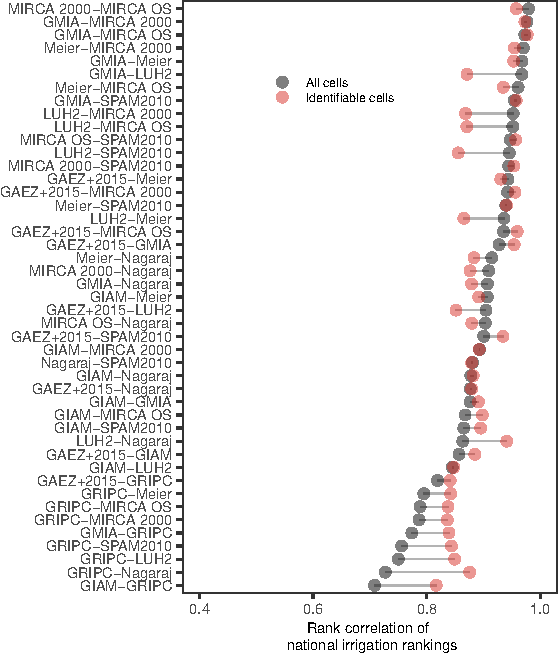
\includegraphics[keepaspectratio]{code_detectability_irrigated_areas_files/figure-latex/rankings_change-1.pdf}}

\begin{Shaded}
\begin{Highlighting}[]
\CommentTok{\# Only for top N countries {-}{-}{-}{-}{-}{-}{-}{-}{-}{-}{-}{-}{-}{-}{-}{-}{-}{-}{-}{-}{-}{-}{-}{-}{-}{-}{-}{-}{-}{-}{-}{-}{-}{-}{-}{-}{-}{-}{-}{-}{-}{-}{-}{-}{-}{-}{-}{-}{-}{-}{-}{-}{-}}

\NormalTok{topN\_overlap\_all[, pair}\SpecialCharTok{:=} \FunctionTok{paste}\NormalTok{(dataset\_1, dataset\_2, }\AttributeTok{sep =} \StringTok{"–"}\NormalTok{)]}
\NormalTok{topN\_overlap\_ident[, pair}\SpecialCharTok{:=} \FunctionTok{paste}\NormalTok{(dataset\_1, dataset\_2, }\AttributeTok{sep =} \StringTok{"–"}\NormalTok{)]}

\NormalTok{topN\_long }\OtherTok{\textless{}{-}} \FunctionTok{rbind}\NormalTok{(topN\_overlap\_all[, .(pair, jaccard\_topN, }\AttributeTok{mode =} \StringTok{"All cells"}\NormalTok{)],}
\NormalTok{                   topN\_overlap\_ident[, .(pair, jaccard\_topN, }\AttributeTok{mode =} \StringTok{"Identifiable cells"}\NormalTok{)])}

\CommentTok{\# order by All{-}cells Jaccard for consistency {-}{-}{-}{-}{-}{-}{-}{-}{-}{-}{-}{-}{-}{-}{-}{-}{-}{-}{-}{-}{-}{-}{-}{-}{-}{-}{-}{-}{-}{-}{-}{-}{-}{-}{-}}

\NormalTok{pair\_order\_topN }\OtherTok{\textless{}{-}}\NormalTok{ topN\_overlap\_all[}\FunctionTok{order}\NormalTok{(jaccard\_topN), pair]}
\NormalTok{topN\_long[, pair}\SpecialCharTok{:=} \FunctionTok{factor}\NormalTok{(pair, }\AttributeTok{levels =}\NormalTok{ pair\_order\_topN)]}

\CommentTok{\# Plot {-}{-}{-}{-}{-}{-}{-}{-}{-}{-}{-}{-}{-}{-}{-}{-}{-}{-}{-}{-}{-}{-}{-}{-}{-}{-}{-}{-}{-}{-}{-}{-}{-}{-}{-}{-}{-}{-}{-}{-}{-}{-}{-}{-}{-}{-}{-}{-}{-}{-}{-}{-}{-}{-}{-}{-}{-}{-}{-}{-}{-}{-}{-}{-}{-}{-}{-}{-}{-}{-}{-}{-}{-}}

\NormalTok{p\_topN }\OtherTok{\textless{}{-}} \FunctionTok{ggplot}\NormalTok{(topN\_long, }\FunctionTok{aes}\NormalTok{(}\AttributeTok{x =}\NormalTok{ jaccard\_topN, }\AttributeTok{y =}\NormalTok{ pair)) }\SpecialCharTok{+}
  \FunctionTok{geom\_segment}\NormalTok{(}\AttributeTok{data =} \FunctionTok{dcast}\NormalTok{(topN\_long, pair }\SpecialCharTok{\textasciitilde{}}\NormalTok{ mode, }\AttributeTok{value.var =} \StringTok{"jaccard\_topN"}\NormalTok{),}
               \FunctionTok{aes}\NormalTok{(}\AttributeTok{x =} \StringTok{\textasciigrave{}}\AttributeTok{All cells}\StringTok{\textasciigrave{}}\NormalTok{, }\AttributeTok{xend =} \StringTok{\textasciigrave{}}\AttributeTok{Identifiable cells}\StringTok{\textasciigrave{}}\NormalTok{,}
                   \AttributeTok{y =}\NormalTok{ pair, }\AttributeTok{yend =}\NormalTok{ pair), }\AttributeTok{inherit.aes =} \ConstantTok{FALSE}\NormalTok{, }\AttributeTok{colour =} \StringTok{"grey70"}\NormalTok{,}
               \AttributeTok{linewidth =} \FloatTok{0.3}\NormalTok{) }\SpecialCharTok{+}
  \FunctionTok{geom\_point}\NormalTok{(}\FunctionTok{aes}\NormalTok{(}\AttributeTok{colour =}\NormalTok{ mode), }\AttributeTok{size =} \DecValTok{2}\NormalTok{, }\AttributeTok{alpha =} \FloatTok{0.5}\NormalTok{) }\SpecialCharTok{+}
  \FunctionTok{scale\_x\_continuous}\NormalTok{(}\AttributeTok{limits =} \FunctionTok{c}\NormalTok{(}\DecValTok{0}\NormalTok{, }\DecValTok{1}\NormalTok{)) }\SpecialCharTok{+}
  \FunctionTok{scale\_color\_manual}\NormalTok{(}\AttributeTok{values =} \FunctionTok{c}\NormalTok{(}\StringTok{"Identifiable cells"} \OtherTok{=} \StringTok{"\#d73027"}\NormalTok{,}
                                \StringTok{"All cells"} \OtherTok{=} \StringTok{"black"}\NormalTok{)) }\SpecialCharTok{+}
  \FunctionTok{labs}\NormalTok{(}\AttributeTok{x =} \StringTok{"Jaccard similarity of }\SpecialCharTok{\textbackslash{}n}\StringTok{ top 20 countries"}\NormalTok{,}
       \AttributeTok{y =} \StringTok{""}\NormalTok{, }\AttributeTok{colour =} \ConstantTok{NULL}\NormalTok{) }\SpecialCharTok{+}
  \FunctionTok{theme\_AP}\NormalTok{() }\SpecialCharTok{+}
  \FunctionTok{theme}\NormalTok{(}\AttributeTok{legend.position =} \StringTok{"none"}\NormalTok{)}

\NormalTok{p\_topN}
\end{Highlighting}
\end{Shaded}

\pandocbounded{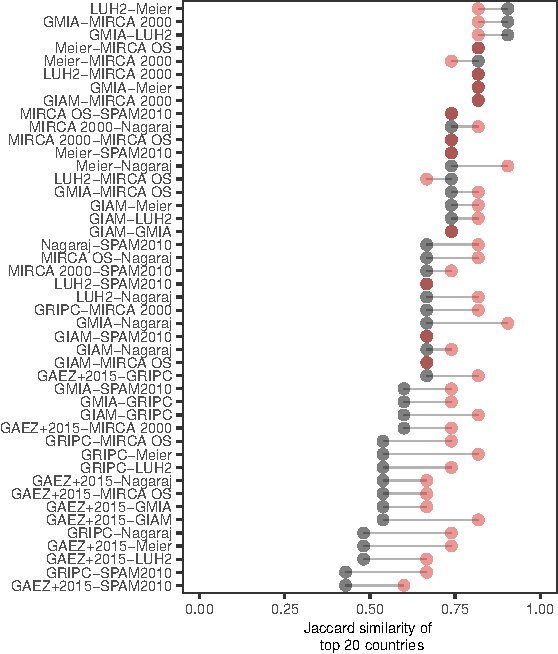
\includegraphics[keepaspectratio]{code_detectability_irrigated_areas_files/figure-latex/rankings_change-2.pdf}}

\begin{Shaded}
\begin{Highlighting}[]
\CommentTok{\# MERGE \#\#\#\#\#\#\#\#\#\#\#\#\#\#\#\#\#\#\#\#\#\#\#\#\#\#\#\#\#\#\#\#\#\#\#\#\#\#\#\#\#\#\#\#\#\#\#\#\#\#\#\#\#\#\#\#\#\#\#\#\#\#\#\#\#\#\#\#\#\#\#\#}

\CommentTok{\# (a) Spearman rank correlation of national total irrigated area rankings for all }
\CommentTok{\# pairwise combinations of datasets. Black points show correlations computed across }
\CommentTok{\# all grid cells, while red points show correlations restricted to identifiable }
\CommentTok{\# cells (i.e., excluding cells where datasets fundamentally disagree on the }
\CommentTok{\# presence of irrigation). Correlations are generally high (0.7–1.0), }
\CommentTok{\# indicating broad agreement in country{-}level rankings. In some cases removing}
\CommentTok{\# disputed cells increases the correlation (red dot to the right of black dot), }
\CommentTok{\# while in others it does not (red dot to the left of black dot)}
\CommentTok{\# }
\CommentTok{\# (b) Jaccard similarity of the top 20 irrigated countries for each dataset pair. }
\CommentTok{\# Black points again denote results using all cells and red points identifiable cells }
\CommentTok{\# only. Most of the time focusing only on identifiable cells increases the}
\CommentTok{\# similarity; meaning that the top 20 become more similar across datasets. In other }
\CommentTok{\# words, once disputed cells are removed there is a more coherent "core" of }
\CommentTok{\# globally dominant irrigation countries. Possibly this is because the strongest}
\CommentTok{\# disagreement disproportionately affect marginal or mid{-}rank countries that}
\CommentTok{\# occassionally enter or leave the top 20 depending on dataset.}

\CommentTok{\# SO: removing disagreeing cells stabilizes who belongs in the top twenty, but not}
\CommentTok{\# necessarily the full ranking hierarchy across al coutnries.}

\FunctionTok{plot\_grid}\NormalTok{(p\_rankcorr, p\_topN, }\AttributeTok{ncol =} \DecValTok{2}\NormalTok{, }\AttributeTok{labels =} \StringTok{"auto"}\NormalTok{)}
\end{Highlighting}
\end{Shaded}

\pandocbounded{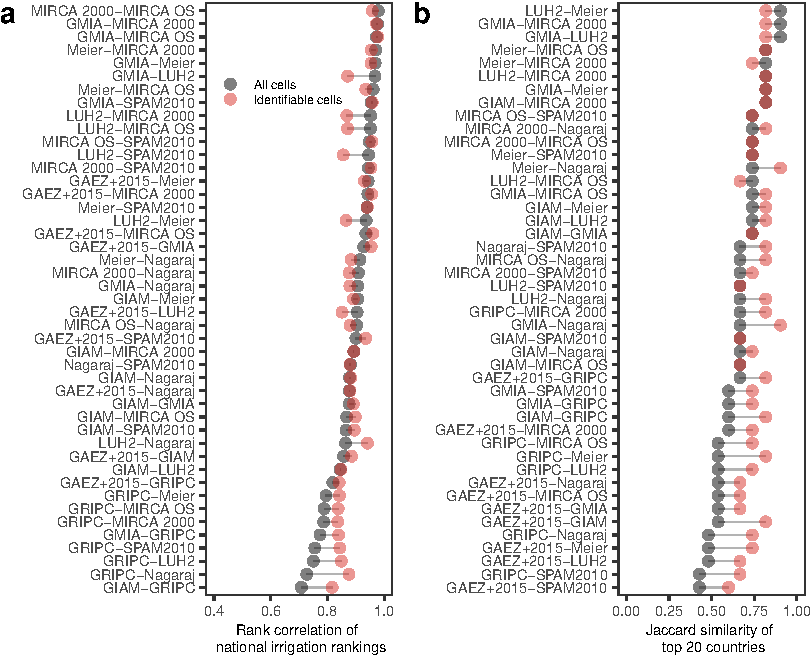
\includegraphics[keepaspectratio]{code_detectability_irrigated_areas_files/figure-latex/merge-1.pdf}}

\subsection{Shift in country ranks}\label{shift-in-country-ranks}

\begin{Shaded}
\begin{Highlighting}[]
\CommentTok{\# SHIFT IN COUNTRY RANKS \#\#\#\#\#\#\#\#\#\#\#\#\#\#\#\#\#\#\#\#\#\#\#\#\#\#\#\#\#\#\#\#\#\#\#\#\#\#\#\#\#\#\#\#\#\#\#\#\#\#\#\#\#\#\#}

\CommentTok{\# Total rank shift {-}{-}{-}{-}{-}{-}{-}{-}{-}{-}{-}{-}{-}{-}{-}{-}{-}{-}{-}{-}{-}{-}{-}{-}{-}{-}{-}{-}{-}{-}{-}{-}{-}{-}{-}{-}{-}{-}{-}{-}{-}{-}{-}{-}{-}{-}{-}{-}{-}{-}{-}{-}{-}{-}{-}{-}{-}{-}{-}{-}{-}}

\NormalTok{rank\_change[, abs\_shift}\SpecialCharTok{:=} \FunctionTok{abs}\NormalTok{(rank\_shift)]}
\NormalTok{rank\_change\_clean }\OtherTok{\textless{}{-}}\NormalTok{ rank\_change[}\SpecialCharTok{!}\FunctionTok{is.na}\NormalTok{(abs\_shift)]}

\CommentTok{\# Histogram of rank shift {-}{-}{-}{-}{-}{-}{-}{-}{-}{-}{-}{-}{-}{-}{-}{-}{-}{-}{-}{-}{-}{-}{-}{-}{-}{-}{-}{-}{-}{-}{-}{-}{-}{-}{-}{-}{-}{-}{-}{-}{-}{-}{-}{-}{-}{-}{-}{-}{-}{-}{-}{-}{-}{-}}

\NormalTok{p\_rankshift\_hist }\OtherTok{\textless{}{-}} \FunctionTok{ggplot}\NormalTok{(rank\_change\_clean, }\FunctionTok{aes}\NormalTok{(abs\_shift)) }\SpecialCharTok{+}
  \FunctionTok{geom\_histogram}\NormalTok{(}\AttributeTok{binwidth =} \DecValTok{1}\NormalTok{, }\AttributeTok{boundary =} \DecValTok{0}\NormalTok{, }\AttributeTok{closed =} \StringTok{"left"}\NormalTok{) }\SpecialCharTok{+}
  \FunctionTok{labs}\NormalTok{(}\AttributeTok{x =} \StringTok{"|Change in national irrigation rank|"}\NormalTok{,}
       \AttributeTok{y =} \StringTok{"Number of country–dataset combinations"}\NormalTok{) }\SpecialCharTok{+}
  \FunctionTok{theme\_AP}\NormalTok{()}

\NormalTok{p\_rankshift\_hist}
\end{Highlighting}
\end{Shaded}

\pandocbounded{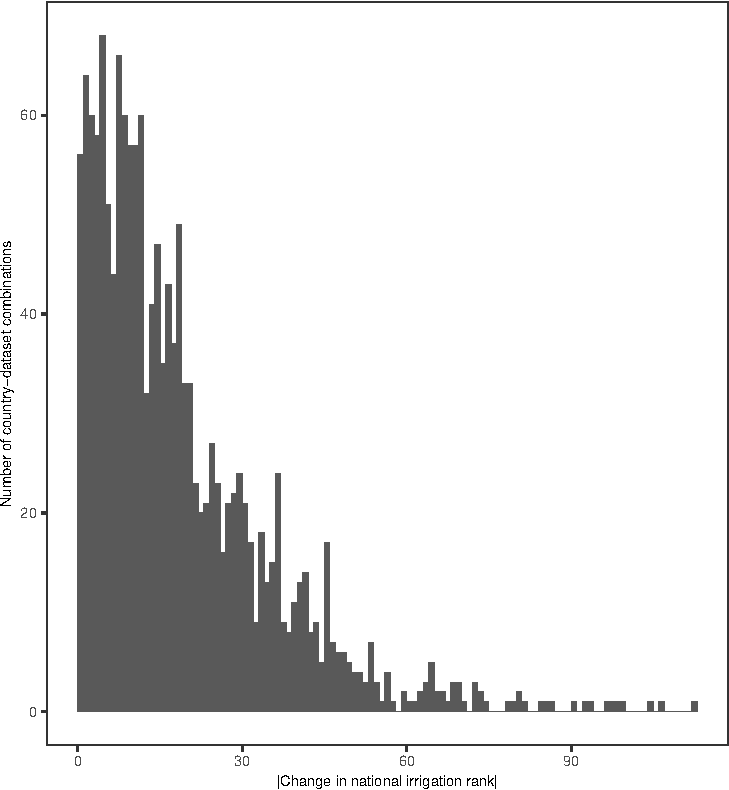
\includegraphics[keepaspectratio]{code_detectability_irrigated_areas_files/figure-latex/shift_country_ranks-1.pdf}}

\begin{Shaded}
\begin{Highlighting}[]
\DocumentationTok{\#\# Cumulative share {-}{-}{-}{-}{-}{-}{-}{-}{-}{-}{-}{-}{-}{-}{-}{-}{-}{-}{-}{-}{-}{-}{-}{-}{-}{-}{-}{-}{-}{-}{-}{-}{-}{-}{-}{-}{-}{-}{-}{-}{-}{-}{-}{-}{-}{-}{-}{-}{-}{-}{-}{-}{-}{-}{-}{-}{-}{-}{-}{-}}

\NormalTok{rank\_shift\_stats }\OtherTok{\textless{}{-}}\NormalTok{ rank\_change\_clean[, .(}\AttributeTok{share\_ge\_1  =} \FunctionTok{mean}\NormalTok{(abs\_shift }\SpecialCharTok{\textgreater{}=} \DecValTok{1}\NormalTok{),}
                                          \AttributeTok{share\_ge\_5  =} \FunctionTok{mean}\NormalTok{(abs\_shift }\SpecialCharTok{\textgreater{}=} \DecValTok{5}\NormalTok{),}
                                          \AttributeTok{share\_ge\_10 =} \FunctionTok{mean}\NormalTok{(abs\_shift }\SpecialCharTok{\textgreater{}=} \DecValTok{10}\NormalTok{), }
                                          \AttributeTok{share\_ge\_20 =} \FunctionTok{mean}\NormalTok{(abs\_shift }\SpecialCharTok{\textgreater{}=} \DecValTok{20}\NormalTok{), }
                                          \AttributeTok{share\_ge\_50 =} \FunctionTok{mean}\NormalTok{(abs\_shift }\SpecialCharTok{\textgreater{}=} \DecValTok{50}\NormalTok{))]}

\NormalTok{rank\_shift\_stats}
\end{Highlighting}
\end{Shaded}

\begin{verbatim}
##    share_ge_1 share_ge_5 share_ge_10 share_ge_20 share_ge_50
##         <num>      <num>       <num>       <num>       <num>
## 1:  0.9641026  0.8038462    0.625641   0.3474359  0.04935897
\end{verbatim}

\begin{Shaded}
\begin{Highlighting}[]
\CommentTok{\# 98.4\% of country–dataset combinations change rank by at least 1 position.}
\CommentTok{\# No country keeps the same rank once we enforce identifiability.}
\CommentTok{\#}
\CommentTok{\# 90\% of countries move by at least 5 rank positions}
\CommentTok{\#}
\CommentTok{\# 71\% of country–dataset combinations move by 10 ranks or more}

\CommentTok{\# FOCUS ON THE SO{-}CALLED "TOP IRRIGATORS" \#\#\#\#\#\#\#\#\#\#\#\#\#\#\#\#\#\#\#\#\#\#\#\#\#\#\#\#\#\#\#\#\#\#\#\#\#}

\NormalTok{number\_countries }\OtherTok{\textless{}{-}} \DecValTok{20}

\CommentTok{\# Countries consistently classified as top irrigators across datasets {-}{-}{-}{-}{-}{-}{-}{-}{-}{-}}

\NormalTok{top10\_all }\OtherTok{\textless{}{-}}\NormalTok{ country\_totals\_all[}\FunctionTok{order}\NormalTok{(rank), .SD[}\DecValTok{1}\SpecialCharTok{:}\NormalTok{number\_countries], dataset] }\SpecialCharTok{\%\textgreater{}\%}
\NormalTok{  .[, .N, by }\OtherTok{=}\NormalTok{ country] }\SpecialCharTok{\%\textgreater{}\%}
\NormalTok{  .[}\SpecialCharTok{!}\NormalTok{country }\SpecialCharTok{==} \StringTok{""}\NormalTok{] }\SpecialCharTok{\%\textgreater{}\%}
\NormalTok{  .[N }\SpecialCharTok{\textgreater{}} \DecValTok{5}\NormalTok{]}

\NormalTok{top10\_all}
\end{Highlighting}
\end{Shaded}

\begin{verbatim}
##           country     N
##            <char> <int>
##  1:         China    10
##  2:         India    10
##  3: United States    10
##  4:      Pakistan    10
##  5:          Iran    10
##  6:        Mexico    10
##  7:        Brazil    10
##  8:         Egypt     8
##  9:        Turkey    10
## 10:    Uzbekistan    10
## 11:         Italy     8
## 12:         Spain    10
## 13:        Russia     6
## 14:    Kazakhstan     8
## 15:      Thailand     8
## 16:    Bangladesh     8
## 17:       Vietnam     8
## 18:     Indonesia     8
## 19:          Iraq     7
\end{verbatim}

\begin{Shaded}
\begin{Highlighting}[]
\CommentTok{\# Also with the median {-}{-}{-}{-}{-}{-}{-}{-}{-}{-}{-}{-}{-}{-}{-}{-}{-}{-}{-}{-}{-}{-}{-}{-}{-}{-}{-}{-}{-}{-}{-}{-}{-}{-}{-}{-}{-}{-}{-}{-}{-}{-}{-}{-}{-}{-}{-}{-}{-}{-}{-}{-}{-}{-}{-}{-}{-}}

\NormalTok{top10\_median }\OtherTok{\textless{}{-}}\NormalTok{ country\_totals\_all[, .(}\AttributeTok{median\_rank =} \FunctionTok{median}\NormalTok{(rank)), country] }\SpecialCharTok{\%\textgreater{}\%}
\NormalTok{  .[}\FunctionTok{order}\NormalTok{(median\_rank)] }\SpecialCharTok{\%\textgreater{}\%}
\NormalTok{  .[}\DecValTok{1}\SpecialCharTok{:}\NormalTok{number\_countries]}

\NormalTok{top10\_median}
\end{Highlighting}
\end{Shaded}

\begin{verbatim}
##           country median_rank
##            <char>       <num>
##  1:         China         1.0
##  2:         India         2.0
##  3: United States         3.0
##  4:      Pakistan         4.0
##  5:          Iran         5.0
##  6:        Mexico         6.5
##  7:     Indonesia         9.0
##  8:      Thailand         9.0
##  9:    Bangladesh        11.0
## 10:        Brazil        11.5
## 11:        Turkey        12.5
## 12:    Uzbekistan        12.5
## 13:       Vietnam        12.5
## 14:         Spain        13.5
## 15:         Egypt        15.0
## 16:         Italy        15.5
## 17:        Russia        15.5
## 18:    Kazakhstan        18.5
## 19:          Iraq        19.5
## 20:     Australia        20.0
##           country median_rank
##            <char>       <num>
\end{verbatim}

\begin{Shaded}
\begin{Highlighting}[]
\CommentTok{\# See change of ranks in countries when only confirmed irrigation is }
\CommentTok{\# accounted for {-}{-}{-}{-}{-}{-}{-}{-}{-}{-}{-}{-}{-}{-}{-}{-}{-}{-}{-}{-}{-}{-}{-}{-}{-}{-}{-}{-}{-}{-}{-}{-}{-}{-}{-}{-}{-}{-}{-}{-}{-}{-}{-}{-}{-}{-}{-}{-}{-}{-}{-}{-}{-}{-}{-}{-}{-}{-}{-}{-}{-}{-}{-}{-}}

\NormalTok{rank\_focus }\OtherTok{\textless{}{-}} \FunctionTok{merge}\NormalTok{(country\_totals\_all[, .(country, dataset, }\AttributeTok{rank\_all =}\NormalTok{ rank)],}
\NormalTok{                    country\_totals\_ident[, .(country, dataset, }\AttributeTok{rank\_ident =}\NormalTok{ rank)],}
                    \AttributeTok{by =} \FunctionTok{c}\NormalTok{(}\StringTok{"country"}\NormalTok{, }\StringTok{"dataset"}\NormalTok{), }\AttributeTok{all =} \ConstantTok{TRUE}\NormalTok{)}

\NormalTok{rank\_focus[, rank\_shift}\SpecialCharTok{:=}\NormalTok{ rank\_ident }\SpecialCharTok{{-}}\NormalTok{ rank\_all]}
\NormalTok{rank\_focus}
\end{Highlighting}
\end{Shaded}

\begin{verbatim}
## Key: <country, dataset>
##             country    dataset rank_all rank_ident rank_shift
##              <char>     <char>    <num>      <num>      <num>
##    1:   Afghanistan  GAEZ+2015     23.0         25          2
##    2:   Afghanistan       GIAM     37.0         23        -14
##    3:   Afghanistan       GMIA     24.0         21         -3
##    4:   Afghanistan      GRIPC     34.0         23        -11
##    5:   Afghanistan       LUH2     21.0         21          0
##   ---                                                        
## 1626: Åland Islands MIRCA 2000    161.5         NA         NA
## 1627: Åland Islands   MIRCA OS    161.0         NA         NA
## 1628: Åland Islands      Meier    150.0         NA         NA
## 1629: Åland Islands    Nagaraj    136.0         NA         NA
## 1630: Åland Islands   SPAM2010    150.0         NA         NA
\end{verbatim}

\begin{Shaded}
\begin{Highlighting}[]
\CommentTok{\# Summarize {-}{-}{-}{-}{-}{-}{-}{-}{-}{-}{-}{-}{-}{-}{-}{-}{-}{-}{-}{-}{-}{-}{-}{-}{-}{-}{-}{-}{-}{-}{-}{-}{-}{-}{-}{-}{-}{-}{-}{-}{-}{-}{-}{-}{-}{-}{-}{-}{-}{-}{-}{-}{-}{-}{-}{-}{-}{-}{-}{-}{-}{-}{-}{-}{-}{-}{-}{-}}

\NormalTok{rank\_focus\_summary }\OtherTok{\textless{}{-}}\NormalTok{ rank\_focus[}\SpecialCharTok{!}\FunctionTok{is.na}\NormalTok{(rank\_ident), .(}\AttributeTok{median\_shift =} \FunctionTok{median}\NormalTok{(rank\_shift, }\AttributeTok{na.rm =} \ConstantTok{TRUE}\NormalTok{),}
                                     \AttributeTok{max\_drop =} \FunctionTok{max}\NormalTok{(rank\_shift, }\AttributeTok{na.rm =} \ConstantTok{TRUE}\NormalTok{),}
                                     \AttributeTok{max\_rise =} \FunctionTok{min}\NormalTok{(rank\_shift, }\AttributeTok{na.rm =} \ConstantTok{TRUE}\NormalTok{),}
                                     \AttributeTok{share\_drop5 =} \FunctionTok{mean}\NormalTok{(rank\_shift }\SpecialCharTok{\textgreater{}=} \DecValTok{5}\NormalTok{, }\AttributeTok{na.rm =} \ConstantTok{TRUE}\NormalTok{),}
                                     \AttributeTok{share\_drop10 =} \FunctionTok{mean}\NormalTok{(rank\_shift }\SpecialCharTok{\textgreater{}=} \DecValTok{10}\NormalTok{, }\AttributeTok{na.rm =} \ConstantTok{TRUE}\NormalTok{)),}
\NormalTok{                                 country] }\SpecialCharTok{\%\textgreater{}\%}
\NormalTok{  .[}\FunctionTok{order}\NormalTok{(}\SpecialCharTok{{-}}\NormalTok{median\_shift)]}

\CommentTok{\# Focus on top 20 irrigation hotspots {-}{-}{-}{-}{-}{-}{-}{-}{-}{-}{-}{-}{-}{-}{-}{-}{-}{-}{-}{-}{-}{-}{-}{-}{-}{-}{-}{-}{-}{-}{-}{-}{-}{-}{-}{-}{-}{-}{-}{-}{-}{-}}

\NormalTok{focus\_countries }\OtherTok{\textless{}{-}}\NormalTok{ top10\_median}\SpecialCharTok{$}\NormalTok{country}
\NormalTok{rank\_focus\_summary[country }\SpecialCharTok{\%in\%}\NormalTok{ focus\_countries]}
\end{Highlighting}
\end{Shaded}

\begin{verbatim}
##           country median_shift max_drop max_rise share_drop5 share_drop10
##            <char>        <num>    <num>    <num>       <num>        <num>
##  1:       Vietnam         39.0       42      -20         0.9          0.9
##  2:     Indonesia         27.0       39      -20         0.9          0.9
##  3:      Thailand         26.0       30      -19         0.9          0.9
##  4:    Bangladesh         25.5       29      -19         0.9          0.9
##  5:        Brazil         14.0       28        8         1.0          0.8
##  6:        Russia          4.0       15       -5         0.4          0.2
##  7:        Mexico          1.5        4       -4         0.0          0.0
##  8:          Iran          1.0        3      -11         0.0          0.0
##  9:         China          0.0        0       -1         0.0          0.0
## 10:         India          0.0        1        0         0.0          0.0
## 11:      Pakistan          0.0        0       -1         0.0          0.0
## 12: United States          0.0        1        0         0.0          0.0
## 13:        Turkey         -1.0        6       -7         0.2          0.0
## 14:     Australia         -2.5       11      -12         0.2          0.1
## 15:    Kazakhstan         -4.0        9      -10         0.2          0.0
## 16:         Spain         -4.0        0       -9         0.0          0.0
## 17:         Italy         -5.5       -3      -11         0.0          0.0
## 18:         Egypt         -7.0       -3      -18         0.0          0.0
## 19:    Uzbekistan         -7.0       -4      -11         0.0          0.0
## 20:          Iraq         -9.5       -2      -12         0.0          0.0
##           country median_shift max_drop max_rise share_drop5 share_drop10
##            <char>        <num>    <num>    <num>       <num>        <num>
\end{verbatim}

\begin{Shaded}
\begin{Highlighting}[]
\CommentTok{\# Positive rank shift: worse rank if only confirmed cells are accounted for.}
\CommentTok{\# Negative rank shift: better rank if only confirmed cells are accounted for.}

\CommentTok{\# {-} median\_shift: median of rank\_shift across datasets.}
\CommentTok{\# {-} max\_drop: maximum worsening (largest positive rank\_shift).}
\CommentTok{\# {-} max\_rise: maximum improvement (most negative rank\_shift).}
\CommentTok{\# {-} share\_drop5: share of dataset cases with rank\_shift \textgreater{}= 5.}
\CommentTok{\# {-} share\_drop10: share with rank\_shift \textgreater{}= 10.}

\CommentTok{\# VIETNAM, BANGLADESH, THAILAND, INDONESIA: in 90\% of cases, Vietnam\textquotesingle{}s rank gets }
\CommentTok{\# at least 10 places worse. Median drop is c. 40 places. Bangladesh, Indonesia, }
\CommentTok{\# Thailand show similar pattern; median shifts of 26{-}27 ranks and 90\% of cases }
\CommentTok{\# with drops larger than 90 ranks.}

\CommentTok{\# CHINA, INDIA, PAKISTAN, USA: Global rank is invariant to whether we use all cells}
\CommentTok{\# or only agreement cells. Irrigated area dominance is robust.}

\CommentTok{\# ITALY, EGYPT, UZBEKISTAN, IRAQ, SPAIN, KAZAKHSTAN: they}
\CommentTok{\# improve their rank when we restrict to confirmed cells; because when we remove}
\CommentTok{\# ambiguous cells in other countries, these countries become more prominent.}

\CommentTok{\# Focus on the countries whose ranking drops the most {-}{-}{-}{-}{-}{-}{-}{-}{-}{-}{-}{-}{-}{-}{-}{-}{-}{-}{-}{-}{-}{-}{-}{-}{-}{-}}

\NormalTok{rank\_focus\_summary[}\FunctionTok{order}\NormalTok{(}\SpecialCharTok{{-}}\NormalTok{median\_shift)][}\DecValTok{1}\SpecialCharTok{:}\NormalTok{number\_countries]}
\end{Highlighting}
\end{Shaded}

\begin{verbatim}
##                  country median_shift max_drop max_rise share_drop5
##                   <char>        <num>    <num>    <num>       <num>
##  1:                Nepal        85.75    112.5     14.0         1.0
##  2:          Philippines        69.00    104.0      5.0         1.0
##  3:   Dominican Republic        64.00     90.0     34.0         1.0
##  4:          Netherlands        58.00    106.5     33.0         1.0
##  5:             Cambodia        46.50     73.5     -3.5         0.9
##  6: United Arab Emirates        44.00     81.0    -29.5         0.8
##  7:              Hungary        40.75     57.5     23.0         1.0
##  8:              Vietnam        39.00     42.0    -20.0         0.9
##  9:             Malaysia        38.50     64.5     -1.0         0.8
## 10:            Guatemala        36.25     68.5    -16.0         0.9
## 11:           Madagascar        35.00     74.5     -1.0         0.9
## 12:                 Mali        35.00     53.5    -14.5         0.7
## 13:             Colombia        34.50     59.5     -3.0         0.9
## 14:             Eswatini        33.50     69.5     -8.5         0.9
## 15:            Venezuela        28.50     66.5      0.0         0.9
## 16:            Indonesia        27.00     39.0    -20.0         0.9
## 17:             Thailand        26.00     30.0    -19.0         0.9
## 18:           Bangladesh        25.50     29.0    -19.0         0.9
## 19:              Germany        25.50     62.5     13.0         1.0
## 20:           Costa Rica        25.00     45.0      1.0         0.9
##                  country median_shift max_drop max_rise share_drop5
##                   <char>        <num>    <num>    <num>       <num>
##     share_drop10
##            <num>
##  1:          1.0
##  2:          0.9
##  3:          1.0
##  4:          1.0
##  5:          0.9
##  6:          0.8
##  7:          1.0
##  8:          0.9
##  9:          0.8
## 10:          0.9
## 11:          0.8
## 12:          0.6
## 13:          0.9
## 14:          0.9
## 15:          0.9
## 16:          0.9
## 17:          0.9
## 18:          0.9
## 19:          1.0
## 20:          0.8
##     share_drop10
##            <num>
\end{verbatim}

\begin{Shaded}
\begin{Highlighting}[]
\CommentTok{\# Plot the results {-}{-}{-}{-}{-}{-}{-}{-}{-}{-}{-}{-}{-}{-}{-}{-}{-}{-}{-}{-}{-}{-}{-}{-}{-}{-}{-}{-}{-}{-}{-}{-}{-}{-}{-}{-}{-}{-}{-}{-}{-}{-}{-}{-}{-}{-}{-}{-}{-}{-}{-}{-}{-}{-}{-}{-}{-}{-}{-}{-}{-}}

\NormalTok{plot\_shift\_ranks }\OtherTok{\textless{}{-}}\NormalTok{ rank\_focus[country }\SpecialCharTok{\%in\%}\NormalTok{ focus\_countries] }\SpecialCharTok{\%\textgreater{}\%}
\NormalTok{  .[, .(country, dataset,}
        \StringTok{\textasciigrave{}}\AttributeTok{All irrigated cells}\StringTok{\textasciigrave{}} \OtherTok{=}\NormalTok{ rank\_all,}
        \StringTok{\textasciigrave{}}\AttributeTok{Confirmed irrigation}\StringTok{\textasciigrave{}} \OtherTok{=}\NormalTok{ rank\_ident)] }\SpecialCharTok{\%\textgreater{}\%}
  \FunctionTok{melt}\NormalTok{(., }\AttributeTok{measure.vars =} \FunctionTok{c}\NormalTok{(}\StringTok{"Confirmed irrigation"}\NormalTok{, }\StringTok{"All irrigated cells"}\NormalTok{)) }\SpecialCharTok{\%\textgreater{}\%}
  \FunctionTok{ggplot}\NormalTok{(., }\FunctionTok{aes}\NormalTok{(dataset, value, }\AttributeTok{color =}\NormalTok{ variable,}
                \AttributeTok{group =} \FunctionTok{interaction}\NormalTok{(country, variable))) }\SpecialCharTok{+}
  \FunctionTok{geom\_line}\NormalTok{(}\AttributeTok{linewidth =} \DecValTok{1}\NormalTok{) }\SpecialCharTok{+}
  \FunctionTok{scale\_y\_reverse}\NormalTok{() }\SpecialCharTok{+}
  \FunctionTok{scale\_color\_manual}\NormalTok{(}\AttributeTok{values =} \FunctionTok{c}\NormalTok{(}\StringTok{"Confirmed irrigation"} \OtherTok{=} \StringTok{"\#d73027"}\NormalTok{,}
                                \StringTok{"All irrigated cells"} \OtherTok{=} \StringTok{"black"}\NormalTok{),}
                     \AttributeTok{name =} \StringTok{""}\NormalTok{) }\SpecialCharTok{+}
  \FunctionTok{scale\_y\_continuous}\NormalTok{(}\AttributeTok{breaks =} \FunctionTok{breaks\_pretty}\NormalTok{(}\AttributeTok{n =} \DecValTok{3}\NormalTok{)) }\SpecialCharTok{+}
  \FunctionTok{facet\_wrap}\NormalTok{(}\SpecialCharTok{\textasciitilde{}}\NormalTok{country) }\SpecialCharTok{+}
  \FunctionTok{labs}\NormalTok{(}\AttributeTok{y =} \StringTok{"National irrigation rank"}\NormalTok{, }\AttributeTok{x =} \ConstantTok{NULL}\NormalTok{) }\SpecialCharTok{+}
  \FunctionTok{coord\_flip}\NormalTok{() }\SpecialCharTok{+}
  \FunctionTok{theme\_AP}\NormalTok{() }\SpecialCharTok{+}
  \FunctionTok{theme}\NormalTok{(}\AttributeTok{legend.position =} \StringTok{"top"}\NormalTok{)}
\end{Highlighting}
\end{Shaded}

\begin{verbatim}
## Scale for y is already present.
## Adding another scale for y, which will replace the existing scale.
\end{verbatim}

\begin{Shaded}
\begin{Highlighting}[]
\NormalTok{plot\_shift\_ranks}
\end{Highlighting}
\end{Shaded}

\pandocbounded{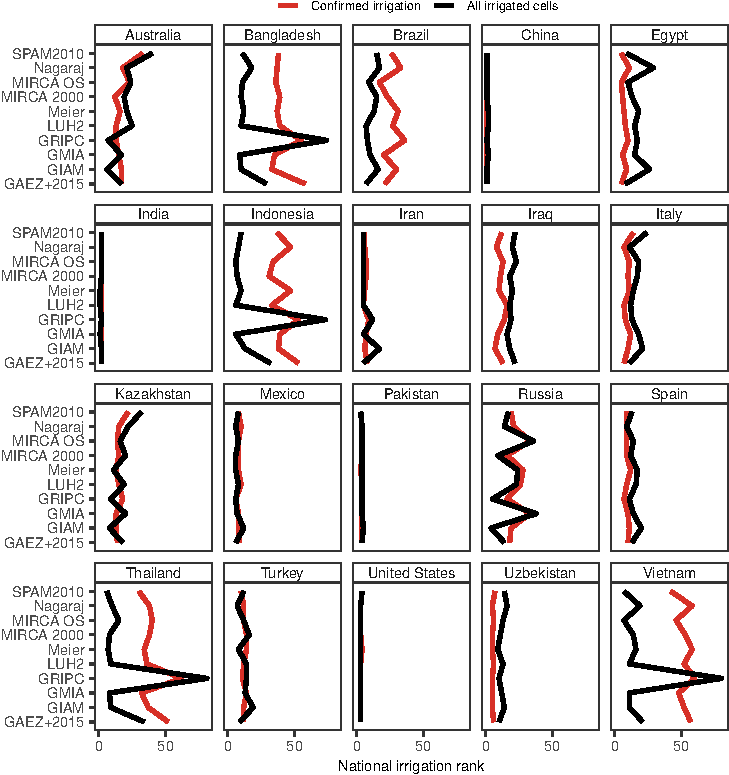
\includegraphics[keepaspectratio]{code_detectability_irrigated_areas_files/figure-latex/shift_country_ranks-2.pdf}}

\begin{Shaded}
\begin{Highlighting}[]
\CommentTok{\# Dashed (red) line much lower than solid (black)}
\CommentTok{\# {-} country drops in rank when ambiguity is removed}
\CommentTok{\# {-} it looks large only because of non{-}identifiable cells}
\CommentTok{\#}
\CommentTok{\# Red equals black}
\CommentTok{\# {-} rank is robust to identifiability}
\CommentTok{\# {-} irrigation signal is spatially coherent}
\CommentTok{\#}
\CommentTok{\# Red above black}
\CommentTok{\# {-} country rises in rank when ambiguity is removed}
\CommentTok{\# {-} it was previously masked by others’ ambiguous irrigation}

\CommentTok{\# If Red and black lines cross across datasets:}
\CommentTok{\# The ordering of countries changes}
\CommentTok{\# Rankings are dataset{-}dependent}
\CommentTok{\# There is no stable hierarchy}
\CommentTok{\# Crossings are visual proof of rank instability.}
\end{Highlighting}
\end{Shaded}

\begin{Shaded}
\begin{Highlighting}[]
\CommentTok{\# COMPUTE AREA RETAINED AND LOST OF TOP 20 COUNTRIES \#\#\#\#\#\#\#\#\#\#\#\#\#\#\#\#\#\#\#\#\#\#\#\#\#\#\#}

\NormalTok{country\_loss }\OtherTok{\textless{}{-}} \FunctionTok{rbindlist}\NormalTok{(}\FunctionTok{lapply}\NormalTok{(new\_dataset\_names, }\ControlFlowTok{function}\NormalTok{(d) \{}

\NormalTok{  dt\_country }\OtherTok{\textless{}{-}}\NormalTok{ dt2[country }\SpecialCharTok{\%in\%}\NormalTok{ top10\_all}\SpecialCharTok{$}\NormalTok{country]}

\NormalTok{  dt\_country[, .(}\AttributeTok{dataset =}\NormalTok{ d,}
                 \AttributeTok{total\_area =} \FunctionTok{sum}\NormalTok{(}\FunctionTok{get}\NormalTok{(d), }\AttributeTok{na.rm =} \ConstantTok{TRUE}\NormalTok{),}
                 \AttributeTok{retained\_area =} \FunctionTok{sum}\NormalTok{(}\FunctionTok{get}\NormalTok{(d)[}\FunctionTok{is.na}\NormalTok{(tau\_max\_ha)], }\AttributeTok{na.rm =} \ConstantTok{TRUE}\NormalTok{),}
                 \AttributeTok{lost\_area =} \FunctionTok{sum}\NormalTok{(}\FunctionTok{get}\NormalTok{(d)[}\SpecialCharTok{!}\FunctionTok{is.na}\NormalTok{(tau\_max\_ha)], }\AttributeTok{na.rm =} \ConstantTok{TRUE}\NormalTok{)),}
\NormalTok{             country]}
\NormalTok{\}))}

\NormalTok{country\_loss[, share\_lost}\SpecialCharTok{:=}\NormalTok{ lost\_area }\SpecialCharTok{/}\NormalTok{ total\_area]}

\CommentTok{\# Compute mean loss per country across datasets to reorder {-}{-}{-}{-}{-}{-}{-}{-}{-}{-}{-}{-}{-}{-}{-}{-}{-}{-}{-}{-}{-}}

\NormalTok{country\_order }\OtherTok{\textless{}{-}}\NormalTok{ country\_loss[, .(}\AttributeTok{mean\_share\_lost =} \FunctionTok{mean}\NormalTok{(share\_lost, }\AttributeTok{na.rm =} \ConstantTok{TRUE}\NormalTok{)),}
\NormalTok{  by }\OtherTok{=}\NormalTok{ country][}\FunctionTok{order}\NormalTok{(}\SpecialCharTok{{-}}\NormalTok{mean\_share\_lost)]  }\CommentTok{\# decreasing order}

\CommentTok{\# Set factor levels in that order{-}{-}{-}{-}{-}{-}{-}{-}{-}{-}{-}{-}{-}{-}{-}{-}{-}{-}{-}{-}{-}{-}{-}{-}{-}{-}{-}{-}{-}{-}{-}{-}{-}{-}{-}{-}{-}{-}{-}{-}{-}{-}{-}{-}{-}{-}{-}}

\NormalTok{country\_loss[, country\_f}\SpecialCharTok{:=} \FunctionTok{factor}\NormalTok{(country, }\AttributeTok{levels =} \FunctionTok{rev}\NormalTok{(country\_order}\SpecialCharTok{$}\NormalTok{country))]}

\CommentTok{\# Plot tileplot {-}{-}{-}{-}{-}{-}{-}{-}{-}{-}{-}{-}{-}{-}{-}{-}{-}{-}{-}{-}{-}{-}{-}{-}{-}{-}{-}{-}{-}{-}{-}{-}{-}{-}{-}{-}{-}{-}{-}{-}{-}{-}{-}{-}{-}{-}{-}{-}{-}{-}{-}{-}{-}{-}{-}{-}{-}{-}{-}{-}{-}{-}{-}{-}}

\NormalTok{plot\_tileplot }\OtherTok{\textless{}{-}} \FunctionTok{ggplot}\NormalTok{(country\_loss, }\FunctionTok{aes}\NormalTok{(dataset, country\_f, }\AttributeTok{fill =}\NormalTok{ share\_lost)) }\SpecialCharTok{+}
  \FunctionTok{geom\_tile}\NormalTok{(}\AttributeTok{color =} \StringTok{"grey90"}\NormalTok{) }\SpecialCharTok{+}
  \FunctionTok{scale\_fill\_gradientn}\NormalTok{(}\AttributeTok{colours =} \FunctionTok{c}\NormalTok{(}\StringTok{"white"}\NormalTok{, }\StringTok{"gold"}\NormalTok{, }\StringTok{"orange"}\NormalTok{, }\StringTok{"red"}\NormalTok{),}
                       \AttributeTok{values  =} \FunctionTok{c}\NormalTok{(}\DecValTok{0}\NormalTok{, }\FloatTok{0.5}\NormalTok{, }\FloatTok{0.8}\NormalTok{, }\DecValTok{1}\NormalTok{),}
                       \AttributeTok{limits  =} \FunctionTok{c}\NormalTok{(}\DecValTok{0}\NormalTok{, }\DecValTok{1}\NormalTok{),}
                       \AttributeTok{name =} \StringTok{"Share of irrigated}\SpecialCharTok{\textbackslash{}n}\StringTok{area lost"}\NormalTok{) }\SpecialCharTok{+}
  \FunctionTok{scale\_y\_discrete}\NormalTok{(}\AttributeTok{name =} \ConstantTok{NULL}\NormalTok{) }\SpecialCharTok{+}
  \FunctionTok{theme\_AP}\NormalTok{() }\SpecialCharTok{+}
  \FunctionTok{labs}\NormalTok{(}\AttributeTok{x =} \StringTok{""}\NormalTok{, }\AttributeTok{y =} \StringTok{""}\NormalTok{) }\SpecialCharTok{+}
  \FunctionTok{theme}\NormalTok{(}\AttributeTok{axis.text.x  =} \FunctionTok{element\_text}\NormalTok{(}\AttributeTok{angle =} \DecValTok{45}\NormalTok{, }\AttributeTok{hjust =} \DecValTok{1}\NormalTok{),}
        \AttributeTok{legend.position =} \StringTok{"right"}\NormalTok{)}

\NormalTok{plot\_tileplot}
\end{Highlighting}
\end{Shaded}

\pandocbounded{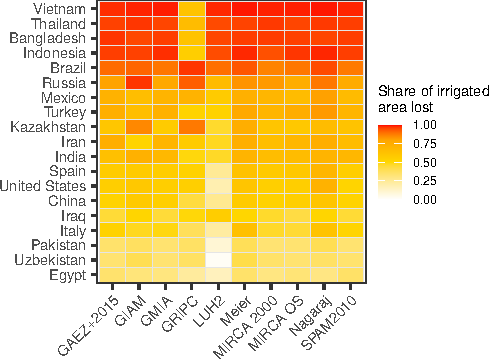
\includegraphics[keepaspectratio]{code_detectability_irrigated_areas_files/figure-latex/plot_tileplot-1.pdf}}

\subsection{Fraction of irrigated areas
lost}\label{fraction-of-irrigated-areas-lost}

\begin{Shaded}
\begin{Highlighting}[]
\CommentTok{\# COLLAPSE ASSESSMENT ACROS A CONTINUUM OF AGREEMENT \#\#\#\#\#\#\#\#\#\#\#\#\#\#\#\#\#\#\#\#\#\#\#\#\#\#\#}

\NormalTok{dt\_share\_lost }\OtherTok{\textless{}{-}} \FunctionTok{dcast}\NormalTok{(dt, lon }\SpecialCharTok{+}\NormalTok{ lat }\SpecialCharTok{+}\NormalTok{ country }\SpecialCharTok{+}\NormalTok{ code }\SpecialCharTok{+}\NormalTok{ continent }\SpecialCharTok{+}\NormalTok{ resolution }\SpecialCharTok{\textasciitilde{}}\NormalTok{ dataset,}
      \AttributeTok{value.var =} \StringTok{"mha"}\NormalTok{)}

\CommentTok{\# Define resolution specific thresholds {-}{-}{-}{-}{-}{-}{-}{-}{-}{-}{-}{-}{-}{-}{-}{-}{-}{-}{-}{-}{-}{-}{-}{-}{-}{-}{-}{-}{-}{-}{-}{-}{-}{-}{-}{-}{-}{-}{-}{-}}

\NormalTok{zero\_tol\_mha\_fun }\OtherTok{\textless{}{-}} \ControlFlowTok{function}\NormalTok{(res) \{}
  \ControlFlowTok{switch}\NormalTok{(res,}
    \StringTok{"0.2deg"} \OtherTok{=} \DecValTok{400}  \SpecialCharTok{/} \FloatTok{1e6}\NormalTok{, }\CommentTok{\# 0.0004 Mha}
    \StringTok{"0.4deg"} \OtherTok{=} \DecValTok{1600} \SpecialCharTok{/} \FloatTok{1e6}\NormalTok{, }\CommentTok{\# 0.0016 Mha}
    \StringTok{"1deg"} \OtherTok{=} \DecValTok{10000} \SpecialCharTok{/} \FloatTok{1e6}\NormalTok{,  }\CommentTok{\# 0.01 Mha}
    \FunctionTok{stop}\NormalTok{(}\StringTok{"Unknown resolution: "}\NormalTok{, res)}
\NormalTok{  )}
\NormalTok{\}}

\CommentTok{\# Make copy just in case {-}{-}{-}{-}{-}{-}{-}{-}{-}{-}{-}{-}{-}{-}{-}{-}{-}{-}{-}{-}{-}{-}{-}{-}{-}{-}{-}{-}{-}{-}{-}{-}{-}{-}{-}{-}{-}{-}{-}{-}{-}{-}{-}{-}{-}{-}{-}{-}{-}{-}{-}{-}{-}{-}{-}}

\NormalTok{dt\_pres }\OtherTok{\textless{}{-}} \FunctionTok{copy}\NormalTok{(dt\_share\_lost)}

\CommentTok{\# Apply resolution{-}specific thresholds {-}{-}{-}{-}{-}{-}{-}{-}{-}{-}{-}{-}{-}{-}{-}{-}{-}{-}{-}{-}{-}{-}{-}{-}{-}{-}{-}{-}{-}{-}{-}{-}{-}{-}{-}{-}{-}{-}{-}{-}{-}}

\NormalTok{dt\_pres[, (dataset\_names) }\SpecialCharTok{:=}\NormalTok{ \{}
\NormalTok{    tol\_mha }\OtherTok{\textless{}{-}} \FunctionTok{zero\_tol\_mha\_fun}\NormalTok{(resolution[}\DecValTok{1}\NormalTok{])}
    \FunctionTok{lapply}\NormalTok{(.SD, }\ControlFlowTok{function}\NormalTok{(x) }\FunctionTok{as.integer}\NormalTok{(x }\SpecialCharTok{\textgreater{}=}\NormalTok{ tol\_mha))}
\NormalTok{    \},}
\NormalTok{    resolution,}
\NormalTok{    .SDcols }\OtherTok{=}\NormalTok{ dataset\_names]}

\CommentTok{\# How many datasets say "irrigated" per cell {-}{-}{-}{-}{-}{-}{-}{-}{-}{-}{-}{-}{-}{-}{-}{-}{-}{-}{-}{-}{-}{-}{-}{-}{-}{-}{-}{-}{-}{-}{-}{-}{-}{-}{-}}

\NormalTok{dt\_pres[, n\_pos}\SpecialCharTok{:=} \FunctionTok{rowSums}\NormalTok{(.SD, }\AttributeTok{na.rm =} \ConstantTok{TRUE}\NormalTok{), .SDcols }\OtherTok{=}\NormalTok{ dataset\_names]}

\NormalTok{n\_datasets }\OtherTok{\textless{}{-}} \FunctionTok{length}\NormalTok{(dataset\_names)  }\CommentTok{\# should be 10}

\CommentTok{\# Melt for k{-}of{-}n agreement {-}{-}{-}{-}{-}{-}{-}{-}{-}{-}{-}{-}{-}{-}{-}{-}{-}{-}{-}{-}{-}{-}{-}{-}{-}{-}{-}{-}{-}{-}{-}{-}{-}{-}{-}{-}{-}{-}{-}{-}{-}{-}{-}{-}{-}{-}{-}{-}{-}{-}{-}{-}}

\NormalTok{grid\_long }\OtherTok{\textless{}{-}} \FunctionTok{melt}\NormalTok{(dt\_pres, }\AttributeTok{id.vars =} \FunctionTok{c}\NormalTok{(}\StringTok{"lon"}\NormalTok{,}\StringTok{"lat"}\NormalTok{,}\StringTok{"country"}\NormalTok{,}\StringTok{"code"}\NormalTok{,}
                    \StringTok{"continent"}\NormalTok{,}\StringTok{"resolution"}\NormalTok{,}\StringTok{"n\_pos"}\NormalTok{),}
                  \AttributeTok{measure.vars =}\NormalTok{ dataset\_names,}
                  \AttributeTok{variable.name =} \StringTok{"dataset"}\NormalTok{,}
                  \AttributeTok{value.name =} \StringTok{"present"}\NormalTok{)}

\CommentTok{\# Run calculations for multiple k (10 down to 5) {-}{-}{-}{-}{-}{-}{-}{-}{-}{-}{-}{-}{-}{-}{-}{-}{-}{-}{-}{-}{-}{-}{-}{-}{-}{-}{-}{-}{-}{-}{-}}

\NormalTok{ks }\OtherTok{\textless{}{-}}\NormalTok{ n\_datasets}\SpecialCharTok{:}\DecValTok{5}
\NormalTok{loss\_by\_k }\OtherTok{\textless{}{-}} \FunctionTok{rbindlist}\NormalTok{(}\FunctionTok{lapply}\NormalTok{(ks, compute\_loss\_for\_k), }\AttributeTok{use.names =} \ConstantTok{TRUE}\NormalTok{)}

\CommentTok{\# Summarize results {-}{-}{-}{-}{-}{-}{-}{-}{-}{-}{-}{-}{-}{-}{-}{-}{-}{-}{-}{-}{-}{-}{-}{-}{-}{-}{-}{-}{-}{-}{-}{-}{-}{-}{-}{-}{-}{-}{-}{-}{-}{-}{-}{-}{-}{-}{-}{-}{-}{-}{-}{-}{-}{-}{-}{-}{-}{-}{-}{-}}

\NormalTok{country\_loss\_by\_k }\OtherTok{\textless{}{-}}\NormalTok{ loss\_by\_k[, .(}\AttributeTok{min  =} \FunctionTok{min}\NormalTok{(share\_lost,  }\AttributeTok{na.rm =} \ConstantTok{TRUE}\NormalTok{),}
                                   \AttributeTok{max  =} \FunctionTok{max}\NormalTok{(share\_lost,  }\AttributeTok{na.rm =} \ConstantTok{TRUE}\NormalTok{),}
                                   \AttributeTok{mean =} \FunctionTok{mean}\NormalTok{(share\_lost, }\AttributeTok{na.rm =} \ConstantTok{TRUE}\NormalTok{)),}
\NormalTok{                               .(country, k)] }\SpecialCharTok{\%\textgreater{}\%}
\NormalTok{  .[, allowed\_disagree}\SpecialCharTok{:=} \DecValTok{10} \SpecialCharTok{{-}}\NormalTok{ k]}

\CommentTok{\# PLOT RESULTS: THE GLOBAL COLLAPSE CURVE \#\#\#\#\#\#\#\#\#\#\#\#\#\#\#\#\#\#\#\#\#\#\#\#\#\#\#\#\#\#\#\#\#\#\#\#\#\#}

\NormalTok{global\_k }\OtherTok{\textless{}{-}}\NormalTok{ country\_loss\_by\_k[, .(}\AttributeTok{mean\_loss   =} \FunctionTok{mean}\NormalTok{(mean, }\AttributeTok{na.rm =} \ConstantTok{TRUE}\NormalTok{),}
                                  \AttributeTok{median\_loss =} \FunctionTok{median}\NormalTok{(mean, }\AttributeTok{na.rm =} \ConstantTok{TRUE}\NormalTok{)), k] }\SpecialCharTok{\%\textgreater{}\%}
\NormalTok{  .[}\FunctionTok{order}\NormalTok{(}\SpecialCharTok{{-}}\NormalTok{k)] }\SpecialCharTok{\%\textgreater{}\%}
\NormalTok{  .[, allowed\_disagree}\SpecialCharTok{:=} \DecValTok{10} \SpecialCharTok{{-}}\NormalTok{ k]}

\FunctionTok{print}\NormalTok{(global\_k)}
\end{Highlighting}
\end{Shaded}

\begin{verbatim}
##        k mean_loss median_loss allowed_disagree
##    <int>     <num>       <num>            <num>
## 1:    10 0.9044568   1.0000000                0
## 2:     9 0.7596387   0.8022176                1
## 3:     8 0.6128174   0.6203836                2
## 4:     7 0.4648955   0.3947794                3
## 5:     6 0.3694552   0.2868750                4
## 6:     5 0.2966630   0.2299499                5
\end{verbatim}

\begin{Shaded}
\begin{Highlighting}[]
\NormalTok{plot\_global\_k }\OtherTok{\textless{}{-}}\NormalTok{ global\_k }\SpecialCharTok{\%\textgreater{}\%}
  \FunctionTok{melt}\NormalTok{(., }\AttributeTok{measure.vars =} \FunctionTok{c}\NormalTok{(}\StringTok{"median\_loss"}\NormalTok{, }\StringTok{"mean\_loss"}\NormalTok{)) }\SpecialCharTok{\%\textgreater{}\%}
  \FunctionTok{ggplot}\NormalTok{(., }\FunctionTok{aes}\NormalTok{(k, value, }\AttributeTok{color =}\NormalTok{ variable)) }\SpecialCharTok{+}
  \FunctionTok{geom\_line}\NormalTok{() }\SpecialCharTok{+}
  \FunctionTok{geom\_point}\NormalTok{()  }\SpecialCharTok{+}
  \FunctionTok{scale\_color\_discrete}\NormalTok{(}\AttributeTok{labels =} \FunctionTok{c}\NormalTok{(}\AttributeTok{median\_loss =} \StringTok{"median"}\NormalTok{, }\AttributeTok{mean\_loss =} \StringTok{"mean"}\NormalTok{),}
                       \AttributeTok{name =} \StringTok{""}\NormalTok{) }\SpecialCharTok{+}
  \FunctionTok{labs}\NormalTok{(}\AttributeTok{x =} \StringTok{"Datasets agreeing"}\NormalTok{, }\AttributeTok{y =} \StringTok{"Fraction irrigation lost"}\NormalTok{) }\SpecialCharTok{+}
  \FunctionTok{theme\_AP}\NormalTok{() }\SpecialCharTok{+}
  \FunctionTok{scale\_x\_reverse}\NormalTok{() }\SpecialCharTok{+}
  \FunctionTok{theme}\NormalTok{(}\AttributeTok{legend.position =} \FunctionTok{c}\NormalTok{(}\FloatTok{0.7}\NormalTok{, }\FloatTok{0.8}\NormalTok{))}

\NormalTok{plot\_global\_k}
\end{Highlighting}
\end{Shaded}

\pandocbounded{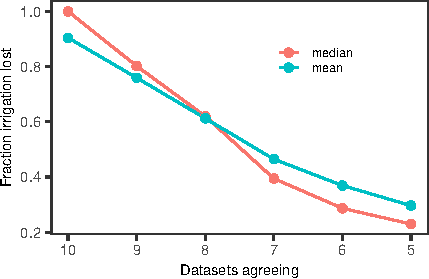
\includegraphics[keepaspectratio]{code_detectability_irrigated_areas_files/figure-latex/fraction_lost_k-1.pdf}}

\begin{Shaded}
\begin{Highlighting}[]
\CommentTok{\# COUNTRY{-}LEVEL COLLAPSE PROFILES \#\#\#\#\#\#\#\#\#\#\#\#\#\#\#\#\#\#\#\#\#\#\#\#\#\#\#\#\#\#\#\#\#\#\#\#\#\#\#\#\#\#\#\#\#\#\#}

\CommentTok{\# Optional: keep only countries with mean loss \textless{} 1 at k=5}

\NormalTok{collapse\_profiles }\OtherTok{\textless{}{-}}\NormalTok{ country\_loss\_by\_k[country }\SpecialCharTok{\%in\%}\NormalTok{ top10\_all}\SpecialCharTok{$}\NormalTok{country] }\SpecialCharTok{\%\textgreater{}\%}
\NormalTok{  .[, allowed\_disagree}\SpecialCharTok{:=} \DecValTok{10} \SpecialCharTok{{-}}\NormalTok{ k]}

\FunctionTok{print}\NormalTok{(collapse\_profiles)}
\end{Highlighting}
\end{Shaded}

\begin{verbatim}
##            country     k         min        max       mean allowed_disagree
##             <char> <int>       <num>      <num>      <num>            <num>
##   1: United States    10 0.473158090 0.85266101 0.75510675                0
##   2:        Mexico    10 0.738049713 0.89044382 0.82904408                0
##   3:        Brazil    10 0.934200459 0.97428230 0.95855641                0
##   4:         Spain    10 0.369426752 0.78995757 0.68156847                0
##   5:         Italy    10 0.464454976 0.76185458 0.65239216                0
##  ---                                                                       
## 110:         China     5 0.003233049 0.08796124 0.04977821                5
## 111:    Bangladesh     5 0.000000000 0.03409091 0.01310055                5
## 112:     Indonesia     5 0.040892193 0.31857555 0.17413988                5
## 113:      Thailand     5 0.000000000 0.13213981 0.05377370                5
## 114:       Vietnam     5 0.000000000 0.10171569 0.03290524                5
\end{verbatim}

\begin{Shaded}
\begin{Highlighting}[]
\NormalTok{plot\_collapse\_profiles }\OtherTok{\textless{}{-}} \FunctionTok{ggplot}\NormalTok{(collapse\_profiles, }\FunctionTok{aes}\NormalTok{(k, mean, }\AttributeTok{group =}\NormalTok{ country,}
                              \AttributeTok{color =}\NormalTok{ country)) }\SpecialCharTok{+}
  \FunctionTok{scale\_color\_discrete}\NormalTok{(}\AttributeTok{name =} \StringTok{""}\NormalTok{) }\SpecialCharTok{+}
  \FunctionTok{geom\_line}\NormalTok{() }\SpecialCharTok{+}
  \FunctionTok{scale\_x\_reverse}\NormalTok{() }\SpecialCharTok{+}
  \FunctionTok{labs}\NormalTok{(}\AttributeTok{x =} \StringTok{"Datasets agreeing"}\NormalTok{, }\AttributeTok{y =} \StringTok{"Fraction irrigation lost"}\NormalTok{) }\SpecialCharTok{+}
  \FunctionTok{theme\_AP}\NormalTok{()}

\NormalTok{plot\_collapse\_profiles}
\end{Highlighting}
\end{Shaded}

\pandocbounded{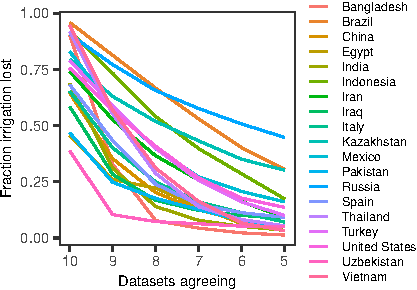
\includegraphics[keepaspectratio]{code_detectability_irrigated_areas_files/figure-latex/fraction_lost_k-2.pdf}}

\begin{Shaded}
\begin{Highlighting}[]
\CommentTok{\# Global distribution by k {-}{-}{-}{-}{-}{-}{-}{-}{-}{-}{-}{-}{-}{-}{-}{-}{-}{-}{-}{-}{-}{-}{-}{-}{-}{-}{-}{-}{-}{-}{-}{-}{-}{-}{-}{-}{-}{-}{-}{-}{-}{-}{-}{-}{-}{-}{-}{-}{-}{-}{-}{-}{-}}

\NormalTok{plot\_curves\_country }\OtherTok{\textless{}{-}} \FunctionTok{ggplot}\NormalTok{(country\_loss\_by\_k, }\FunctionTok{aes}\NormalTok{(mean, }\AttributeTok{color =} \FunctionTok{factor}\NormalTok{(k), }\AttributeTok{group =}\NormalTok{ k)) }\SpecialCharTok{+}
  \FunctionTok{geom\_density}\NormalTok{() }\SpecialCharTok{+}
  \FunctionTok{labs}\NormalTok{(}\AttributeTok{x =} \StringTok{"Fraction irrigation lost"}\NormalTok{, }\AttributeTok{y =} \StringTok{"Density"}\NormalTok{, }\AttributeTok{color =} \StringTok{"Datasets }\SpecialCharTok{\textbackslash{}n}\StringTok{agreeing"}\NormalTok{) }\SpecialCharTok{+}
  \FunctionTok{theme\_AP}\NormalTok{() }\SpecialCharTok{+}
  \FunctionTok{theme}\NormalTok{(}\AttributeTok{legend.position =} \StringTok{"right"}\NormalTok{) }\SpecialCharTok{+}
  \FunctionTok{scale\_x\_continuous}\NormalTok{(}\AttributeTok{breaks =}\NormalTok{ scales}\SpecialCharTok{::}\FunctionTok{breaks\_pretty}\NormalTok{(}\AttributeTok{n =} \DecValTok{3}\NormalTok{)) }\SpecialCharTok{+}
  \FunctionTok{scale\_color\_viridis\_d}\NormalTok{(}\AttributeTok{option =} \StringTok{"mako"}\NormalTok{, }\AttributeTok{direction =} \SpecialCharTok{{-}}\DecValTok{1}\NormalTok{)}

\NormalTok{plot\_curves\_country}
\end{Highlighting}
\end{Shaded}

\pandocbounded{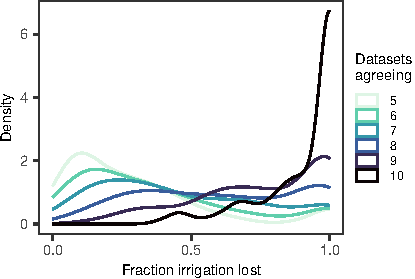
\includegraphics[keepaspectratio]{code_detectability_irrigated_areas_files/figure-latex/fraction_lost_k-3.pdf}}

\begin{Shaded}
\begin{Highlighting}[]
\CommentTok{\# MERGE \#\#\#\#\#\#\#\#\#\#\#\#\#\#\#\#\#\#\#\#\#\#\#\#\#\#\#\#\#\#\#\#\#\#\#\#\#\#\#\#\#\#\#\#\#\#\#\#\#\#\#\#\#\#\#\#\#\#\#\#\#\#\#\#\#\#\#\#\#\#\#\#}

\NormalTok{left }\OtherTok{\textless{}{-}} \FunctionTok{plot\_grid}\NormalTok{(plot\_global\_k, plot\_curves\_country, }\AttributeTok{ncol =} \DecValTok{1}\NormalTok{, }\AttributeTok{labels =} \StringTok{"auto"}\NormalTok{, }
                  \AttributeTok{rel\_heights =} \FunctionTok{c}\NormalTok{(}\FloatTok{0.6}\NormalTok{, }\FloatTok{0.4}\NormalTok{))}
\FunctionTok{plot\_grid}\NormalTok{(left, plot\_collapse\_profiles, }\AttributeTok{ncol =} \DecValTok{2}\NormalTok{, }\AttributeTok{labels =} \FunctionTok{c}\NormalTok{(}\StringTok{""}\NormalTok{, }\StringTok{"c"}\NormalTok{),}
          \AttributeTok{rel\_widths =} \FunctionTok{c}\NormalTok{(}\FloatTok{0.35}\NormalTok{, }\FloatTok{0.65}\NormalTok{))}
\end{Highlighting}
\end{Shaded}

\pandocbounded{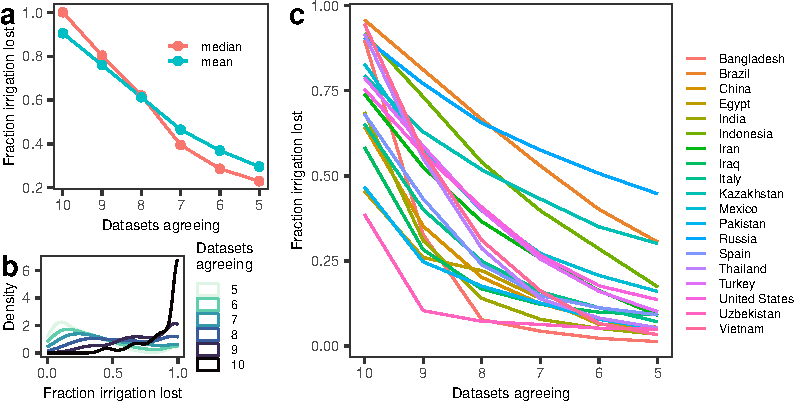
\includegraphics[keepaspectratio]{code_detectability_irrigated_areas_files/figure-latex/merge_k-1.pdf}}

\begin{Shaded}
\begin{Highlighting}[]
\CommentTok{\# PLOTS SHOWING K{-}OF{-}10 AGREEMENT \#\#\#\#\#\#\#\#\#\#\#\#\#\#\#\#\#\#\#\#\#\#\#\#\#\#\#\#\#\#\#\#\#\#\#\#\#\#\#\#\#\#\#\#\#\#}

\CommentTok{\# Prepare data {-}{-}{-}{-}{-}{-}{-}{-}{-}{-}{-}{-}{-}{-}{-}{-}{-}{-}{-}{-}{-}{-}{-}{-}{-}{-}{-}{-}{-}{-}{-}{-}{-}{-}{-}{-}{-}{-}{-}{-}{-}{-}{-}{-}{-}{-}{-}{-}{-}{-}{-}{-}{-}{-}{-}{-}{-}{-}{-}{-}{-}{-}{-}{-}{-}}

\NormalTok{dt\_plot }\OtherTok{\textless{}{-}}\NormalTok{ dt\_pres[, .N, .(resolution, n\_pos)]}
\NormalTok{dt\_plot[, frac}\SpecialCharTok{:=}\NormalTok{ N }\SpecialCharTok{/} \FunctionTok{sum}\NormalTok{(N), by }\OtherTok{=}\NormalTok{ resolution]}

\CommentTok{\# Fraction of cells in the consensus core (\textgreater{}=9/10) {-}{-}{-}{-}{-}{-}{-}{-}{-}{-}{-}{-}{-}{-}{-}{-}{-}{-}{-}{-}{-}{-}{-}{-}{-}{-}{-}{-}{-}}

\NormalTok{dt\_plot[}\FunctionTok{order}\NormalTok{(n\_pos)] }\SpecialCharTok{\%\textgreater{}\%}
\NormalTok{  .[n\_pos }\SpecialCharTok{\textgreater{}=} \DecValTok{9}\NormalTok{] }\SpecialCharTok{\%\textgreater{}\%}
\NormalTok{  .[, }\FunctionTok{sum}\NormalTok{(frac), resolution]}
\end{Highlighting}
\end{Shaded}

\begin{verbatim}
##    resolution        V1
##        <char>     <num>
## 1:       1deg 0.2119707
## 2:     0.4deg 0.1843615
## 3:     0.2deg 0.1429349
\end{verbatim}

\begin{Shaded}
\begin{Highlighting}[]
\CommentTok{\# Fraction of cells irrigated by less than half of the datasets .{-}{-}{-}{-}{-}{-}{-}{-}{-}{-}{-}{-}{-}{-}{-}}

\NormalTok{dt\_plot[}\FunctionTok{order}\NormalTok{(n\_pos)] }\SpecialCharTok{\%\textgreater{}\%}
\NormalTok{  .[n\_pos }\SpecialCharTok{\textless{}} \DecValTok{5} \SpecialCharTok{\&}\NormalTok{ n\_pos }\SpecialCharTok{!=} \DecValTok{0}\NormalTok{] }\SpecialCharTok{\%\textgreater{}\%}
\NormalTok{  .[, }\FunctionTok{sum}\NormalTok{(frac), resolution]}
\end{Highlighting}
\end{Shaded}

\begin{verbatim}
##    resolution        V1
##        <char>     <num>
## 1:     0.2deg 0.3014845
## 2:     0.4deg 0.2681645
## 3:       1deg 0.2144542
\end{verbatim}

\begin{Shaded}
\begin{Highlighting}[]
\CommentTok{\# Compute statistics {-}{-}{-}{-}{-}{-}{-}{-}{-}{-}{-}{-}{-}{-}{-}{-}{-}{-}{-}{-}{-}{-}{-}{-}{-}{-}{-}{-}{-}{-}{-}{-}{-}{-}{-}{-}{-}{-}{-}{-}{-}{-}{-}{-}{-}{-}{-}{-}{-}{-}{-}{-}{-}{-}{-}{-}{-}{-}{-}}

\NormalTok{dt\_summary }\OtherTok{\textless{}{-}}\NormalTok{ dt\_plot[, .(}\AttributeTok{total =} \FunctionTok{sum}\NormalTok{(N),}
                          \AttributeTok{absence =} \FunctionTok{sum}\NormalTok{(N[n\_pos }\SpecialCharTok{==} \DecValTok{0}\NormalTok{]),}
                          \AttributeTok{contested =} \FunctionTok{sum}\NormalTok{(N[n\_pos }\SpecialCharTok{\textgreater{}=}\DecValTok{1} \SpecialCharTok{\&}\NormalTok{ n\_pos }\SpecialCharTok{\textless{}=}\DecValTok{8}\NormalTok{]),}
                          \AttributeTok{presence =} \FunctionTok{sum}\NormalTok{(N[n\_pos }\SpecialCharTok{\textgreater{}=}\DecValTok{9}\NormalTok{])), }
\NormalTok{                      resolution]}

\NormalTok{dt\_summary[, }\StringTok{\textasciigrave{}}\AttributeTok{:=}\StringTok{\textasciigrave{}}\NormalTok{(}\AttributeTok{frac\_absence =}\NormalTok{ absence }\SpecialCharTok{/}\NormalTok{ total,}
                  \AttributeTok{frac\_contested =}\NormalTok{ contested }\SpecialCharTok{/}\NormalTok{ total,}
                  \AttributeTok{frac\_presence =}\NormalTok{ presence }\SpecialCharTok{/}\NormalTok{ total)]}

\NormalTok{dt\_summary}
\end{Highlighting}
\end{Shaded}

\begin{verbatim}
##    resolution  total absence contested presence frac_absence frac_contested
##        <char>  <int>   <int>     <int>    <int>        <num>          <num>
## 1:       1deg   8053    3515      2831     1707    0.4364833      0.3515460
## 2:     0.2deg 128660   43227     67043    18390    0.3359785      0.5210866
## 3:     0.4deg  39569   14634     17640     7295    0.3698350      0.4458035
##    frac_presence
##            <num>
## 1:     0.2119707
## 2:     0.1429349
## 3:     0.1843615
\end{verbatim}

\begin{Shaded}
\begin{Highlighting}[]
\CommentTok{\# Probability that a dataset detects irrigation in a given cell {-}{-}{-}{-}{-}{-}{-}{-}{-}{-}{-}{-}{-}{-}{-}{-}}

\NormalTok{dt\_k }\OtherTok{\textless{}{-}}\NormalTok{ dt\_pres[, .N, .(resolution, n\_pos)]}

\NormalTok{dt\_prob }\OtherTok{\textless{}{-}}\NormalTok{ dt\_k[, .(}\AttributeTok{mean\_k =} \FunctionTok{weighted.mean}\NormalTok{(n\_pos, N),}
                    \AttributeTok{detection\_prob =} \FunctionTok{weighted.mean}\NormalTok{(n\_pos, N) }\SpecialCharTok{/} \DecValTok{10}\NormalTok{), }
\NormalTok{                resolution]}

\NormalTok{dt\_prob}
\end{Highlighting}
\end{Shaded}

\begin{verbatim}
##    resolution   mean_k detection_prob
##        <char>    <num>          <num>
## 1:       1deg 3.359866      0.3359866
## 2:     0.2deg 3.379776      0.3379776
## 3:     0.4deg 3.449898      0.3449898
\end{verbatim}

\begin{Shaded}
\begin{Highlighting}[]
\CommentTok{\# In how many cells do fewer than half of the datasets detect irrigation? {-}{-}{-}{-}{-}{-}}

\NormalTok{dt\_weak }\OtherTok{\textless{}{-}}\NormalTok{ dt\_k[, .(}\AttributeTok{total\_cells =} \FunctionTok{sum}\NormalTok{(N),}
  \AttributeTok{no\_irrigation =} \FunctionTok{sum}\NormalTok{(N[n\_pos }\SpecialCharTok{==} \DecValTok{0}\NormalTok{]),}
  \AttributeTok{any\_irrigation =} \FunctionTok{sum}\NormalTok{(N[n\_pos }\SpecialCharTok{\textgreater{}=} \DecValTok{1}\NormalTok{]),}
  \AttributeTok{weak\_detection =} \FunctionTok{sum}\NormalTok{(N[n\_pos }\SpecialCharTok{\textgreater{}=} \DecValTok{1} \SpecialCharTok{\&}\NormalTok{ n\_pos }\SpecialCharTok{\textless{}=} \DecValTok{5}\NormalTok{])), resolution]}

\NormalTok{dt\_weak[, }\StringTok{\textasciigrave{}}\AttributeTok{:=}\StringTok{\textasciigrave{}}\NormalTok{(}\AttributeTok{frac\_weak\_all =}\NormalTok{ weak\_detection }\SpecialCharTok{/}\NormalTok{ total\_cells,}
               \AttributeTok{frac\_weak\_given\_any =}\NormalTok{ weak\_detection }\SpecialCharTok{/}\NormalTok{ any\_irrigation)]}

\NormalTok{dt\_weak}
\end{Highlighting}
\end{Shaded}

\begin{verbatim}
##    resolution total_cells no_irrigation any_irrigation weak_detection
##        <char>       <int>         <int>          <int>          <int>
## 1:       1deg        8053          3515           4538           1931
## 2:     0.2deg      128660         43227          85433          43489
## 3:     0.4deg       39569         14634          24935          11758
##    frac_weak_all frac_weak_given_any
##            <num>               <num>
## 1:     0.2397864           0.4255178
## 2:     0.3380149           0.5090422
## 3:     0.2971518           0.4715460
\end{verbatim}

\begin{Shaded}
\begin{Highlighting}[]
\CommentTok{\# Plot distribution {-}{-}{-}{-}{-}{-}{-}{-}{-}{-}{-}{-}{-}{-}{-}{-}{-}{-}{-}{-}{-}{-}{-}{-}{-}{-}{-}{-}{-}{-}{-}{-}{-}{-}{-}{-}{-}{-}{-}{-}{-}{-}{-}{-}{-}{-}{-}{-}{-}{-}{-}{-}{-}{-}{-}{-}{-}{-}{-}{-}}

\NormalTok{p1 }\OtherTok{\textless{}{-}}\NormalTok{ plot\_agreement }\OtherTok{\textless{}{-}} \FunctionTok{ggplot}\NormalTok{(dt\_plot, }\FunctionTok{aes}\NormalTok{(n\_pos, frac)) }\SpecialCharTok{+}
  \FunctionTok{geom\_col}\NormalTok{() }\SpecialCharTok{+}
  \FunctionTok{facet\_wrap}\NormalTok{(}\SpecialCharTok{\textasciitilde{}}\NormalTok{resolution) }\SpecialCharTok{+}
  \FunctionTok{labs}\NormalTok{(}\AttributeTok{x =} \StringTok{"Datasets agreeing"}\NormalTok{,}
       \AttributeTok{y =} \StringTok{"Fraction of cells"}\NormalTok{) }\SpecialCharTok{+}
  \FunctionTok{theme\_AP}\NormalTok{()}

\NormalTok{p1}
\end{Highlighting}
\end{Shaded}

\pandocbounded{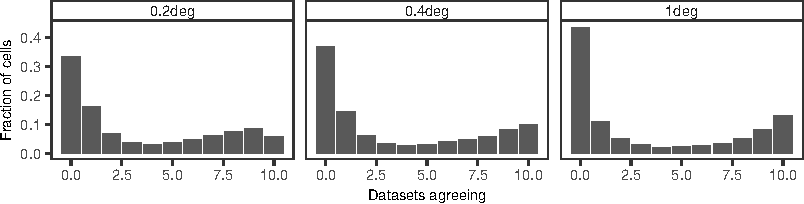
\includegraphics[keepaspectratio]{code_detectability_irrigated_areas_files/figure-latex/plot_agreement-1.pdf}}

\begin{Shaded}
\begin{Highlighting}[]
\CommentTok{\# Prepare data for cumulative plot {-}{-}{-}{-}{-}{-}{-}{-}{-}{-}{-}{-}{-}{-}{-}{-}{-}{-}{-}{-}{-}{-}{-}{-}{-}{-}{-}{-}{-}{-}{-}{-}{-}{-}{-}{-}{-}{-}{-}{-}{-}{-}{-}{-}{-}}

\NormalTok{dt\_ecdf }\OtherTok{\textless{}{-}}\NormalTok{ dt\_pres[, .N, .(resolution, n\_pos)]}
\NormalTok{dt\_ecdf[, frac}\SpecialCharTok{:=}\NormalTok{ N }\SpecialCharTok{/} \FunctionTok{sum}\NormalTok{(N), resolution]}
\FunctionTok{setorder}\NormalTok{(dt\_ecdf, resolution, n\_pos)}
\NormalTok{dt\_ecdf[, cdf}\SpecialCharTok{:=} \FunctionTok{cumsum}\NormalTok{(frac), resolution]}

\NormalTok{dt\_ecdf[, resolution}\SpecialCharTok{:=} \FunctionTok{factor}\NormalTok{(resolution, }\AttributeTok{levels =} \FunctionTok{c}\NormalTok{(}\StringTok{"0.2deg"}\NormalTok{,}\StringTok{"0.4deg"}\NormalTok{,}\StringTok{"1deg"}\NormalTok{))]}

\CommentTok{\# Plot {-}{-}{-}{-}{-}{-}{-}{-}{-}{-}{-}{-}{-}{-}{-}{-}{-}{-}{-}{-}{-}{-}{-}{-}{-}{-}{-}{-}{-}{-}{-}{-}{-}{-}{-}{-}{-}{-}{-}{-}{-}{-}{-}{-}{-}{-}{-}{-}{-}{-}{-}{-}{-}{-}{-}{-}{-}{-}{-}{-}{-}{-}{-}{-}{-}{-}{-}{-}{-}{-}{-}{-}{-}}

\NormalTok{p2 }\OtherTok{\textless{}{-}} \FunctionTok{ggplot}\NormalTok{(dt\_ecdf, }\FunctionTok{aes}\NormalTok{(n\_pos, cdf, }\AttributeTok{colour =}\NormalTok{ resolution)) }\SpecialCharTok{+}
  \FunctionTok{geom\_step}\NormalTok{(}\AttributeTok{linewidth =} \FloatTok{0.8}\NormalTok{) }\SpecialCharTok{+}
  \FunctionTok{scale\_x\_continuous}\NormalTok{(}\AttributeTok{breaks =} \DecValTok{0}\SpecialCharTok{:}\DecValTok{10}\NormalTok{) }\SpecialCharTok{+}
  \FunctionTok{scale\_color\_manual}\NormalTok{(}\AttributeTok{values =}\NormalTok{ res\_palette, }\AttributeTok{name =} \StringTok{""}\NormalTok{) }\SpecialCharTok{+}
  \FunctionTok{labs}\NormalTok{(}\AttributeTok{x =} \StringTok{"Datasets agreeing"}\NormalTok{, }\AttributeTok{y =} \StringTok{"Cum. grid cells"}\NormalTok{,}
       \AttributeTok{colour =} \StringTok{"Resolution"}\NormalTok{) }\SpecialCharTok{+}
  \FunctionTok{theme\_AP}\NormalTok{() }\SpecialCharTok{+}
  \FunctionTok{theme}\NormalTok{(}\AttributeTok{legend.position =} \FunctionTok{c}\NormalTok{(}\FloatTok{0.7}\NormalTok{, }\FloatTok{0.3}\NormalTok{))}

\NormalTok{p2}
\end{Highlighting}
\end{Shaded}

\pandocbounded{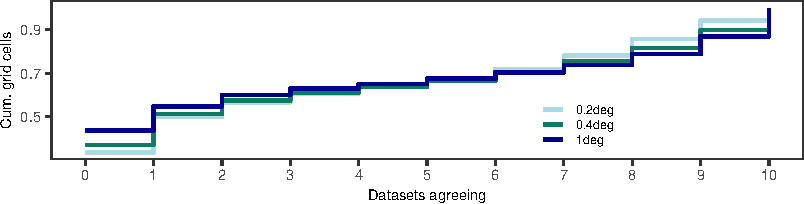
\includegraphics[keepaspectratio]{code_detectability_irrigated_areas_files/figure-latex/plot_agreement-2.pdf}}

\begin{Shaded}
\begin{Highlighting}[]
\FunctionTok{plot\_grid}\NormalTok{(p1, p2, }\AttributeTok{ncol =} \DecValTok{2}\NormalTok{, }\AttributeTok{rel\_widths =} \FunctionTok{c}\NormalTok{(}\FloatTok{0.7}\NormalTok{, }\FloatTok{0.3}\NormalTok{), }\AttributeTok{labels =} \StringTok{"auto"}\NormalTok{)}
\end{Highlighting}
\end{Shaded}

\pandocbounded{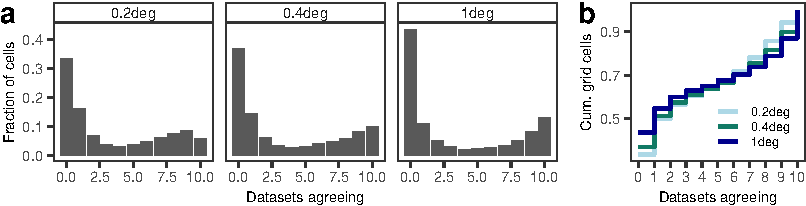
\includegraphics[keepaspectratio]{code_detectability_irrigated_areas_files/figure-latex/plot_agreement-3.pdf}}

\begin{Shaded}
\begin{Highlighting}[]
\CommentTok{\# Plot: consensus regime plot {-}{-}{-}{-}{-}{-}{-}{-}{-}{-}{-}{-}{-}{-}{-}{-}{-}{-}{-}{-}{-}{-}{-}{-}{-}{-}{-}{-}{-}{-}{-}{-}{-}{-}{-}{-}{-}{-}{-}{-}{-}{-}{-}{-}{-}{-}{-}{-}{-}{-}}

\NormalTok{dt\_regime }\OtherTok{\textless{}{-}}\NormalTok{ dt\_k[, .(}\AttributeTok{absence =} \FunctionTok{sum}\NormalTok{(N[n\_pos }\SpecialCharTok{==} \DecValTok{0}\NormalTok{]),}
                      \AttributeTok{contested =} \FunctionTok{sum}\NormalTok{(N[n\_pos }\SpecialCharTok{\textgreater{}=} \DecValTok{1} \SpecialCharTok{\&}\NormalTok{ n\_pos }\SpecialCharTok{\textless{}=} \DecValTok{8}\NormalTok{]),}
                      \AttributeTok{presence =} \FunctionTok{sum}\NormalTok{(N[n\_pos }\SpecialCharTok{\textgreater{}=} \DecValTok{9}\NormalTok{])), resolution]}

\NormalTok{dt\_regime }\OtherTok{\textless{}{-}} \FunctionTok{melt}\NormalTok{(dt\_regime, }\AttributeTok{id.vars =} \StringTok{"resolution"}\NormalTok{, }\AttributeTok{variable.name =} \StringTok{"regime"}\NormalTok{,}
                  \AttributeTok{value.name =} \StringTok{"N"}\NormalTok{)}

\NormalTok{dt\_regime[, frac}\SpecialCharTok{:=}\NormalTok{ N }\SpecialCharTok{/} \FunctionTok{sum}\NormalTok{(N), by }\OtherTok{=}\NormalTok{ resolution]}

\NormalTok{plot\_regime }\OtherTok{\textless{}{-}} \FunctionTok{ggplot}\NormalTok{(dt\_regime, }\FunctionTok{aes}\NormalTok{(resolution, frac, }\AttributeTok{fill =}\NormalTok{ regime)) }\SpecialCharTok{+}
  \FunctionTok{geom\_col}\NormalTok{(}\AttributeTok{width =} \FloatTok{0.7}\NormalTok{) }\SpecialCharTok{+}
  \FunctionTok{scale\_fill\_manual}\NormalTok{(}\AttributeTok{values =} \FunctionTok{c}\NormalTok{(}\AttributeTok{absence =} \StringTok{"\#4D4D4D"}\NormalTok{,}
                               \AttributeTok{contested =} \StringTok{"\#E69F00"}\NormalTok{,}
                               \AttributeTok{presence =} \StringTok{"\#0072B2"}\NormalTok{), }
                    \AttributeTok{guide =} \FunctionTok{guide\_legend}\NormalTok{(}\AttributeTok{nrow =} \DecValTok{3}\NormalTok{), }
                    \AttributeTok{name =} \StringTok{"Agreement }\SpecialCharTok{\textbackslash{}n}\StringTok{regime"}\NormalTok{) }\SpecialCharTok{+}
  \FunctionTok{labs}\NormalTok{(}\AttributeTok{x =} \ConstantTok{NULL}\NormalTok{, }\AttributeTok{y =} \StringTok{"Fraction of cells"}\NormalTok{) }\SpecialCharTok{+}
  \FunctionTok{theme\_AP}\NormalTok{() }\SpecialCharTok{+}
  \FunctionTok{theme}\NormalTok{(}\AttributeTok{legend.position =} \StringTok{"top"}\NormalTok{)}
  

\NormalTok{plot\_regime}
\end{Highlighting}
\end{Shaded}

\pandocbounded{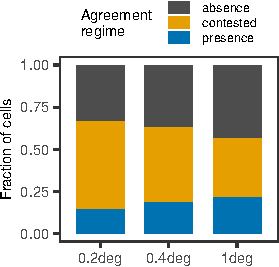
\includegraphics[keepaspectratio]{code_detectability_irrigated_areas_files/figure-latex/plot_agreement2-1.pdf}}

\newpage

\section{Consequences for crop production, water and
climate}\label{consequences-for-crop-production-water-and-climate}

\begin{Shaded}
\begin{Highlighting}[]
\CommentTok{\# GLOBAL CROP PRODUCTION UDNER DIFFERENT AGREEMENT RULES \#\#\#\#\#\#\#\#\#\#\#\#\#\#\#\#\#\#\#\#\#\#\#}
\DocumentationTok{\#\#\#\#\#\#\#\#\#\#\#\#\#\#\#\#\#\#\#\#\#\#\#\#\#\#\#\#\#\#\#\#\#\#\#\#\#\#\#\#\#\#\#\#\#\#\#\#\#\#\#\#\#\#\#\#\#\#\#\#\#\#\#\#\#\#\#\#\#\#\#\#\#\#\#\#\#\#\#\#}

\CommentTok{\# Read crop datasets {-}{-}{-}{-}{-}{-}{-}{-}{-}{-}{-}{-}{-}{-}{-}{-}{-}{-}{-}{-}{-}{-}{-}{-}{-}{-}{-}{-}{-}{-}{-}{-}{-}{-}{-}{-}{-}{-}{-}{-}{-}{-}{-}{-}{-}{-}{-}{-}{-}{-}{-}{-}{-}{-}{-}{-}{-}{-}{-}}

\NormalTok{gaez\_crops\_02\_aligned }\OtherTok{\textless{}{-}} \FunctionTok{fread}\NormalTok{(}\StringTok{"./datasets/crops/gaez2015\_crops\_irrigated\_0p2deg\_aligned.csv"}\NormalTok{)}
\NormalTok{gaez\_crops\_04\_aligned }\OtherTok{\textless{}{-}} \FunctionTok{fread}\NormalTok{(}\StringTok{"./datasets/crops/gaez2015\_crops\_irrigated\_0p4deg\_aligned.csv"}\NormalTok{)}
\NormalTok{gaez\_crops\_1\_aligned }\OtherTok{\textless{}{-}} \FunctionTok{fread}\NormalTok{(}\StringTok{"./datasets/crops/gaez2015\_crops\_irrigated\_1deg\_aligned.csv"}\NormalTok{)}

\CommentTok{\# Extract crop cols{-}{-}{-}{-}{-}{-}{-}{-}{-}{-}{-}{-}{-}{-}{-}{-}{-}{-}{-}{-}{-}{-}{-}{-}{-}{-}{-}{-}{-}{-}{-}{-}{-}{-}{-}{-}{-}{-}{-}{-}{-}{-}{-}{-}{-}{-}{-}{-}{-}{-}{-}{-}{-}{-}{-}{-}{-}{-}{-}{-}{-}}

\NormalTok{crop\_cols }\OtherTok{\textless{}{-}} \FunctionTok{setdiff}\NormalTok{(}\FunctionTok{names}\NormalTok{(gaez\_crops\_02\_aligned),   }
                     \FunctionTok{c}\NormalTok{(}\StringTok{"lon"}\NormalTok{, }\StringTok{"lat"}\NormalTok{, }\StringTok{"country"}\NormalTok{, }\StringTok{"code"}\NormalTok{, }\StringTok{"continent"}\NormalTok{))}

\CommentTok{\# Run for all grids {-}{-}{-}{-}{-}{-}{-}{-}{-}{-}{-}{-}{-}{-}{-}{-}{-}{-}{-}{-}{-}{-}{-}{-}{-}{-}{-}{-}{-}{-}{-}{-}{-}{-}{-}{-}{-}{-}{-}{-}{-}{-}{-}{-}{-}{-}{-}{-}{-}{-}{-}{-}{-}{-}{-}{-}{-}{-}{-}{-}}

\NormalTok{res\_list }\OtherTok{\textless{}{-}} \FunctionTok{list}\NormalTok{(}\StringTok{"0.2deg"} \OtherTok{=}\NormalTok{ gaez\_crops\_02\_aligned,}
                 \StringTok{"0.4deg"} \OtherTok{=}\NormalTok{ gaez\_crops\_04\_aligned,}
                 \StringTok{"1deg"}   \OtherTok{=}\NormalTok{ gaez\_crops\_1\_aligned)}

\NormalTok{results }\OtherTok{\textless{}{-}} \FunctionTok{lapply}\NormalTok{(}\FunctionTok{names}\NormalTok{(res\_list), }\ControlFlowTok{function}\NormalTok{(r) \{}
  \FunctionTok{run\_prod\_analysis}\NormalTok{(r, res\_list[[r]], dt\_pres, crop\_cols)}
\NormalTok{\})}
\end{Highlighting}
\end{Shaded}

\begin{verbatim}
## Warning in melt.data.table(prod_agreement_wide, id.vars = "k", variable.name =
## "crop", : 'measure.vars' [banana, barley, cassava, cotton, ...] are not all of
## the same type. By order of hierarchy, the molten data value column will be of
## type 'double'. All measure variables not of type 'double' will be coerced too.
## Check DETAILS in ?melt.data.table for more on coercion.
## Warning in melt.data.table(prod_agreement_wide, id.vars = "k", variable.name =
## "crop", : 'measure.vars' [banana, barley, cassava, cotton, ...] are not all of
## the same type. By order of hierarchy, the molten data value column will be of
## type 'double'. All measure variables not of type 'double' will be coerced too.
## Check DETAILS in ?melt.data.table for more on coercion.
## Warning in melt.data.table(prod_agreement_wide, id.vars = "k", variable.name =
## "crop", : 'measure.vars' [banana, barley, cassava, cotton, ...] are not all of
## the same type. By order of hierarchy, the molten data value column will be of
## type 'double'. All measure variables not of type 'double' will be coerced too.
## Check DETAILS in ?melt.data.table for more on coercion.
\end{verbatim}

\begin{Shaded}
\begin{Highlighting}[]
\NormalTok{crop\_all  }\OtherTok{\textless{}{-}} \FunctionTok{rbindlist}\NormalTok{(}\FunctionTok{lapply}\NormalTok{(results, }\StringTok{\textasciigrave{}}\AttributeTok{[[}\StringTok{\textasciigrave{}}\NormalTok{, }\StringTok{"crop"}\NormalTok{))}
\NormalTok{total\_all }\OtherTok{\textless{}{-}} \FunctionTok{rbindlist}\NormalTok{(}\FunctionTok{lapply}\NormalTok{(results, }\StringTok{\textasciigrave{}}\AttributeTok{[[}\StringTok{\textasciigrave{}}\NormalTok{, }\StringTok{"total"}\NormalTok{))}

\NormalTok{total\_all}
\end{Highlighting}
\end{Shaded}

\begin{verbatim}
##         k total_production frac_vs_5  loss_vs_5 resolution
##     <int>            <num>     <num>      <num>     <char>
##  1:    10          1169573 0.3202186 0.67978144     0.2deg
##  2:     9          2502525 0.6851690 0.31483100     0.2deg
##  3:     8          3134409 0.8581734 0.14182663     0.2deg
##  4:     7          3419707 0.9362854 0.06371456     0.2deg
##  5:     6          3566546 0.9764886 0.02351138     0.2deg
##  6:     5          3652420 1.0000000 0.00000000     0.2deg
##  7:    10          1871731 0.5108121 0.48918792     0.4deg
##  8:     9          2984702 0.8145518 0.18544818     0.4deg
##  9:     8          3311908 0.9038492 0.09615082     0.4deg
## 10:     7          3494139 0.9535818 0.04641816     0.4deg
## 11:     6          3603949 0.9835498 0.01645020     0.4deg
## 12:     5          3664226 1.0000000 0.00000000     0.4deg
## 13:    10          2130581 0.5602983 0.43970167       1deg
## 14:     9          3204009 0.8425876 0.15741241       1deg
## 15:     8          3516376 0.9247335 0.07526646       1deg
## 16:     7          3648597 0.9595049 0.04049508       1deg
## 17:     6          3724181 0.9793817 0.02061829       1deg
## 18:     5          3802583 1.0000000 0.00000000       1deg
\end{verbatim}

\begin{Shaded}
\begin{Highlighting}[]
\CommentTok{\# PLOT \#\#\#\#\#\#\#\#\#\#\#\#\#\#\#\#\#\#\#\#\#\#\#\#\#\#\#\#\#\#\#\#\#\#\#\#\#\#\#\#\#\#\#\#\#\#\#\#\#\#\#\#\#\#\#\#\#\#\#\#\#\#\#\#\#\#\#\#\#\#\#\#\#}

\CommentTok{\# Heatmap {-}{-}{-}{-}{-}{-}{-}{-}{-}{-}{-}{-}{-}{-}{-}{-}{-}{-}{-}{-}{-}{-}{-}{-}{-}{-}{-}{-}{-}{-}{-}{-}{-}{-}{-}{-}{-}{-}{-}{-}{-}{-}{-}{-}{-}{-}{-}{-}{-}{-}{-}{-}{-}{-}{-}{-}{-}{-}{-}{-}{-}{-}{-}{-}{-}{-}{-}{-}{-}{-}}

\NormalTok{plot\_dt }\OtherTok{\textless{}{-}}\NormalTok{ crop\_all[}\SpecialCharTok{!}\FunctionTok{is.na}\NormalTok{(frac\_vs\_5)]}

\CommentTok{\# Fix merged crop names only {-}{-}{-}{-}{-}{-}{-}{-}{-}{-}{-}{-}{-}{-}{-}{-}{-}{-}{-}{-}{-}{-}{-}{-}{-}{-}{-}{-}{-}{-}{-}{-}{-}{-}{-}{-}{-}{-}{-}{-}{-}{-}{-}{-}{-}{-}{-}{-}{-}{-}{-}}

\NormalTok{plot\_dt[, crop}\SpecialCharTok{:=} \FunctionTok{gsub}\NormalTok{(}\StringTok{"potatoandsweetpotato"}\NormalTok{, }\StringTok{"potato \& sweet potato"}\NormalTok{, crop)]}
\NormalTok{plot\_dt[, crop}\SpecialCharTok{:=} \FunctionTok{gsub}\NormalTok{(}\StringTok{"yamsandotherroots"}\NormalTok{, }\StringTok{"yams \& other roots"}\NormalTok{, crop)]}
\NormalTok{plot\_dt[, crop}\SpecialCharTok{:=} \FunctionTok{gsub}\NormalTok{(}\StringTok{"oilpalmfruit"}\NormalTok{, }\StringTok{"oil palm fruit"}\NormalTok{, crop)]}
\NormalTok{plot\_dt[, crop}\SpecialCharTok{:=} \FunctionTok{gsub}\NormalTok{(}\StringTok{"sugarbeet"}\NormalTok{, }\StringTok{"sugar beet"}\NormalTok{, crop)]}
\NormalTok{plot\_dt[, crop}\SpecialCharTok{:=} \FunctionTok{gsub}\NormalTok{(}\StringTok{"sugarcane"}\NormalTok{, }\StringTok{"sugar cane"}\NormalTok{, crop)]}
\NormalTok{plot\_dt[, crop}\SpecialCharTok{:=} \FunctionTok{gsub}\NormalTok{(}\StringTok{"othercereals"}\NormalTok{, }\StringTok{"other cereals"}\NormalTok{, crop)]}
\NormalTok{plot\_dt[, crop}\SpecialCharTok{:=} \FunctionTok{gsub}\NormalTok{(}\StringTok{"foddercrops"}\NormalTok{, }\StringTok{"fodder crops"}\NormalTok{, crop)]}
\NormalTok{plot\_dt[, crop}\SpecialCharTok{:=} \FunctionTok{gsub}\NormalTok{(}\StringTok{"cropsnes"}\NormalTok{, }\StringTok{"crops n.e.s."}\NormalTok{, crop)]}

\NormalTok{plot\_dt[, k}\SpecialCharTok{:=} \FunctionTok{factor}\NormalTok{(k, }\AttributeTok{levels =} \DecValTok{10}\SpecialCharTok{:}\DecValTok{5}\NormalTok{)]}

\NormalTok{plot\_heatmap }\OtherTok{\textless{}{-}} \FunctionTok{ggplot}\NormalTok{(plot\_dt, }\FunctionTok{aes}\NormalTok{(}\AttributeTok{x =}\NormalTok{ k, }\AttributeTok{y =}\NormalTok{ crop, }\AttributeTok{fill =}\NormalTok{ loss\_vs\_5)) }\SpecialCharTok{+}
  \FunctionTok{geom\_tile}\NormalTok{(}\AttributeTok{color =} \StringTok{"white"}\NormalTok{) }\SpecialCharTok{+}
  \FunctionTok{scale\_fill\_gradientn}\NormalTok{(}\AttributeTok{colours =} \FunctionTok{c}\NormalTok{(}\StringTok{"green"}\NormalTok{, }\StringTok{"yellow"}\NormalTok{, }\StringTok{"orange"}\NormalTok{, }\StringTok{"red"}\NormalTok{),}
                       \AttributeTok{values =} \FunctionTok{c}\NormalTok{(}\DecValTok{0}\NormalTok{, }\FloatTok{0.5}\NormalTok{, }\DecValTok{1}\NormalTok{),}
                       \AttributeTok{breaks =} \FunctionTok{c}\NormalTok{(}\DecValTok{0}\NormalTok{, }\FloatTok{0.5}\NormalTok{, }\DecValTok{1}\NormalTok{),}
                       \AttributeTok{name    =} \StringTok{"Fraction production }\SpecialCharTok{\textbackslash{}n}\StringTok{lost"}\NormalTok{) }\SpecialCharTok{+}
  \FunctionTok{facet\_wrap}\NormalTok{(}\SpecialCharTok{\textasciitilde{}}\NormalTok{resolution, }\AttributeTok{ncol =} \DecValTok{3}\NormalTok{) }\SpecialCharTok{+}
  \FunctionTok{labs}\NormalTok{(}\AttributeTok{x =} \StringTok{"Datasets agreeing"}\NormalTok{,}
       \AttributeTok{y =} \ConstantTok{NULL}\NormalTok{) }\SpecialCharTok{+}
  \FunctionTok{theme\_AP}\NormalTok{() }\SpecialCharTok{+}
  \FunctionTok{theme}\NormalTok{(}\AttributeTok{axis.text.y =} \FunctionTok{element\_text}\NormalTok{(}\AttributeTok{size =} \DecValTok{7}\NormalTok{),}
        \AttributeTok{legend.position =} \StringTok{"top"}\NormalTok{)}

\NormalTok{plot\_heatmap}
\end{Highlighting}
\end{Shaded}

\pandocbounded{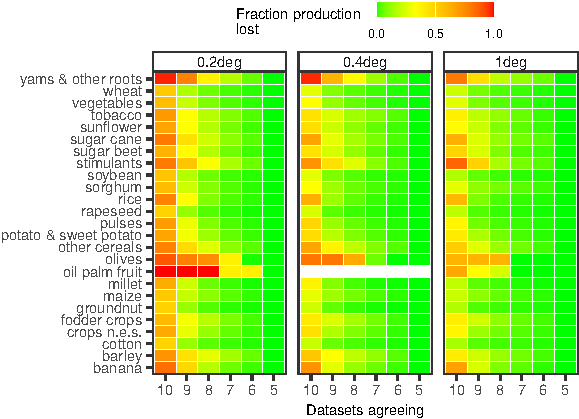
\includegraphics[keepaspectratio]{code_detectability_irrigated_areas_files/figure-latex/crop_consequences-1.pdf}}

\begin{Shaded}
\begin{Highlighting}[]
\CommentTok{\# Global production {-}{-}{-}{-}{-}{-}{-}{-}{-}{-}{-}{-}{-}{-}{-}{-}{-}{-}{-}{-}{-}{-}{-}{-}{-}{-}{-}{-}{-}{-}{-}{-}{-}{-}{-}{-}{-}{-}{-}{-}{-}{-}{-}{-}{-}{-}{-}{-}{-}{-}{-}{-}{-}{-}{-}{-}{-}{-}{-}{-}}

\NormalTok{plot\_crop\_total }\OtherTok{\textless{}{-}} \FunctionTok{ggplot}\NormalTok{(total\_all,}
       \FunctionTok{aes}\NormalTok{(}\AttributeTok{x =}\NormalTok{ k, }\AttributeTok{y =}\NormalTok{ loss\_vs\_5, }\AttributeTok{group =}\NormalTok{ resolution, }\AttributeTok{color =}\NormalTok{ resolution)) }\SpecialCharTok{+}
  \FunctionTok{geom\_line}\NormalTok{() }\SpecialCharTok{+}
  \FunctionTok{geom\_point}\NormalTok{() }\SpecialCharTok{+}
  \FunctionTok{scale\_color\_manual}\NormalTok{(}\AttributeTok{values =}\NormalTok{ res\_palette) }\SpecialCharTok{+}
  \FunctionTok{scale\_x\_reverse}\NormalTok{(}\AttributeTok{breaks =} \DecValTok{10}\SpecialCharTok{:}\DecValTok{5}\NormalTok{) }\SpecialCharTok{+}
  \FunctionTok{scale\_y\_continuous}\NormalTok{(}\AttributeTok{labels =}\NormalTok{ scales}\SpecialCharTok{::}\FunctionTok{percent\_format}\NormalTok{(}\AttributeTok{accuracy =} \DecValTok{1}\NormalTok{)) }\SpecialCharTok{+}
  \FunctionTok{labs}\NormalTok{(}\AttributeTok{x =} \StringTok{"Datasets agreeing"}\NormalTok{, }\AttributeTok{y =} \StringTok{"Fraction production lost"}\NormalTok{,}
       \AttributeTok{color =} \StringTok{"Resolution"}\NormalTok{) }\SpecialCharTok{+}
  \FunctionTok{theme\_AP}\NormalTok{() }\SpecialCharTok{+}
  \FunctionTok{theme}\NormalTok{(}\AttributeTok{legend.position =} \FunctionTok{c}\NormalTok{(}\FloatTok{0.7}\NormalTok{, }\FloatTok{0.7}\NormalTok{))}

\NormalTok{plot\_crop\_total}
\end{Highlighting}
\end{Shaded}

\pandocbounded{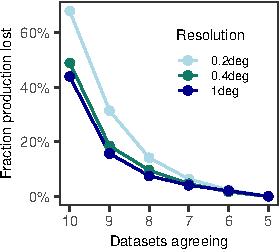
\includegraphics[keepaspectratio]{code_detectability_irrigated_areas_files/figure-latex/global_production-1.pdf}}

\subsection{Effect on global
breadbaskets}\label{effect-on-global-breadbaskets}

\begin{Shaded}
\begin{Highlighting}[]
\CommentTok{\# COMPUTE BREADBASKETS \#\#\#\#\#\#\#\#\#\#\#\#\#\#\#\#\#\#\#\#\#\#\#\#\#\#\#\#\#\#\#\#\#\#\#\#\#\#\#\#\#\#\#\#\#\#\#\#\#\#\#\#\#\#\#\#\#}
\DocumentationTok{\#\#\#\#\#\#\#\#\#\#\#\#\#\#\#\#\#\#\#\#\#\#\#\#\#\#\#\#\#\#\#\#\#\#\#\#\#\#\#\#\#\#\#\#\#\#\#\#\#\#\#\#\#\#\#\#\#\#\#\#\#\#\#\#\#\#\#\#\#\#\#\#\#\#\#\#\#\#\#\#}

\CommentTok{\# LAND SEA MASK {-}{-}{-}{-}{-}{-}{-}{-}{-}{-}{-}{-}{-}{-}{-}{-}{-}{-}{-}{-}{-}{-}{-}{-}{-}{-}{-}{-}{-}{-}{-}{-}{-}{-}{-}{-}{-}{-}{-}{-}{-}{-}{-}{-}{-}{-}{-}{-}{-}{-}{-}{-}{-}{-}{-}{-}{-}{-}{-}{-}{-}{-}{-}{-}{-}}

\NormalTok{grain\_crops }\OtherTok{\textless{}{-}} \FunctionTok{intersect}\NormalTok{(}\FunctionTok{c}\NormalTok{(}\StringTok{"wheat"}\NormalTok{, }\StringTok{"rice"}\NormalTok{, }\StringTok{"maize"}\NormalTok{, }\StringTok{"barley"}\NormalTok{, }\StringTok{"millet"}\NormalTok{,}
                           \StringTok{"sorghum"}\NormalTok{, }\StringTok{"othercereals"}\NormalTok{), }\FunctionTok{names}\NormalTok{(gaez\_crops\_02\_aligned))}

\NormalTok{lon\_min }\OtherTok{\textless{}{-}} \FunctionTok{min}\NormalTok{(gaez\_crops\_02\_aligned}\SpecialCharTok{$}\NormalTok{lon)}
\NormalTok{lon\_max }\OtherTok{\textless{}{-}} \FunctionTok{max}\NormalTok{(gaez\_crops\_02\_aligned}\SpecialCharTok{$}\NormalTok{lon)}
\NormalTok{lat\_min }\OtherTok{\textless{}{-}} \FunctionTok{min}\NormalTok{(gaez\_crops\_02\_aligned}\SpecialCharTok{$}\NormalTok{lat)}
\NormalTok{lat\_max }\OtherTok{\textless{}{-}} \FunctionTok{max}\NormalTok{(gaez\_crops\_02\_aligned}\SpecialCharTok{$}\NormalTok{lat)}

\NormalTok{template }\OtherTok{\textless{}{-}} \FunctionTok{rast}\NormalTok{(}\AttributeTok{xmin =}\NormalTok{ lon\_min, }\AttributeTok{xmax =}\NormalTok{ lon\_max,}
                 \AttributeTok{ymin =}\NormalTok{ lat\_min, }\AttributeTok{ymax =}\NormalTok{ lat\_max,}
                 \AttributeTok{resolution =} \FloatTok{0.2}\NormalTok{,}
                 \AttributeTok{crs =} \StringTok{"EPSG:4326"}\NormalTok{)}

\NormalTok{world }\OtherTok{\textless{}{-}} \FunctionTok{vect}\NormalTok{(spData}\SpecialCharTok{::}\NormalTok{world)}
\NormalTok{land\_mask }\OtherTok{\textless{}{-}} \FunctionTok{rasterize}\NormalTok{(world, template, }\AttributeTok{field =} \DecValTok{1}\NormalTok{, }\AttributeTok{background =} \ConstantTok{NA}\NormalTok{)}

\CommentTok{\# Focus regions {-}{-}{-}{-}{-}{-}{-}{-}{-}{-}{-}{-}{-}{-}{-}{-}{-}{-}{-}{-}{-}{-}{-}{-}{-}{-}{-}{-}{-}{-}{-}{-}{-}{-}{-}{-}{-}{-}{-}{-}{-}{-}{-}{-}{-}{-}{-}{-}{-}{-}{-}{-}{-}{-}{-}{-}{-}{-}{-}{-}{-}{-}{-}{-}}

\CommentTok{\# PREVIOUS LAND MASK EXCLUDES WATER BODIES IN THE AREAS \#\#\#\#\#\#\#\#\#\#\#\#\#\#\#\#\#\#\#\#\#\#\#\#}

\CommentTok{\# India: Indus Valley (Pakistan) and the Ganges Delta (Bangladesh).}
\CommentTok{\# China: Hebei{-}Henan{-}Shandong axis}
\CommentTok{\# USA: Ogallala Box; the Nebraska{-}to{-}Texas irrigation corridor.}
\CommentTok{\# Egypt: Egyptian Nile}
\CommentTok{\# Mediterranean: Spain, Italy, Greece, Turkey and North Africa}

\NormalTok{regions }\OtherTok{\textless{}{-}} \FunctionTok{list}\NormalTok{(}\StringTok{"Indo{-}Gangetic Plain"} \OtherTok{=} \FunctionTok{ext}\NormalTok{(}\DecValTok{68}\NormalTok{, }\DecValTok{91}\NormalTok{, }\FloatTok{21.5}\NormalTok{, }\DecValTok{33}\NormalTok{),}
                \StringTok{"North China Plain"} \OtherTok{=} \FunctionTok{ext}\NormalTok{(}\DecValTok{113}\NormalTok{, }\DecValTok{121}\NormalTok{, }\DecValTok{34}\NormalTok{, }\DecValTok{41}\NormalTok{),}
                \StringTok{"US High Plains"} \OtherTok{=} \FunctionTok{ext}\NormalTok{(}\SpecialCharTok{{-}}\DecValTok{104}\NormalTok{, }\SpecialCharTok{{-}}\DecValTok{96}\NormalTok{, }\DecValTok{32}\NormalTok{, }\DecValTok{44}\NormalTok{),}
                \StringTok{"Nile Delta/Basin"} \OtherTok{=} \FunctionTok{ext}\NormalTok{(}\FloatTok{29.5}\NormalTok{, }\DecValTok{33}\NormalTok{, }\DecValTok{24}\NormalTok{, }\FloatTok{31.5}\NormalTok{),}
                \StringTok{"Mekong Delta"} \OtherTok{=} \FunctionTok{ext}\NormalTok{(}\FloatTok{104.5}\NormalTok{, }\FloatTok{106.5}\NormalTok{, }\FloatTok{8.5}\NormalTok{, }\FloatTok{11.5}\NormalTok{),}
                \StringTok{"Mediterranean Basin"} \OtherTok{=} \FunctionTok{ext}\NormalTok{(}\SpecialCharTok{{-}}\DecValTok{6}\NormalTok{, }\DecValTok{36}\NormalTok{, }\DecValTok{30}\NormalTok{, }\DecValTok{46}\NormalTok{))}

\CommentTok{\# Run for 0.2, 0.4, 1{-}{-}{-}{-}{-}{-}{-}{-}{-}{-}{-}{-}{-}{-}{-}{-}{-}{-}{-}{-}{-}{-}{-}{-}{-}{-}{-}{-}{-}{-}{-}{-}{-}{-}{-}{-}{-}{-}{-}{-}{-}{-}{-}{-}{-}{-}{-}{-}{-}{-}{-}{-}{-}{-}{-}{-}{-}{-}{-}}

\NormalTok{res\_list }\OtherTok{\textless{}{-}} \FunctionTok{list}\NormalTok{(}\StringTok{"0.2deg"} \OtherTok{=}\NormalTok{ gaez\_crops\_02\_aligned,}
                 \StringTok{"0.4deg"} \OtherTok{=}\NormalTok{ gaez\_crops\_04\_aligned,}
                 \StringTok{"1deg"}   \OtherTok{=}\NormalTok{ gaez\_crops\_1\_aligned)}

\NormalTok{results\_regions\_all }\OtherTok{\textless{}{-}} \FunctionTok{rbindlist}\NormalTok{(}
  \FunctionTok{lapply}\NormalTok{(}\FunctionTok{names}\NormalTok{(res\_list), }\ControlFlowTok{function}\NormalTok{(r) \{}
    \FunctionTok{compute\_breadbaskets}\NormalTok{(}
      \AttributeTok{res\_tag =}\NormalTok{ r,}
      \AttributeTok{crops\_aligned =}\NormalTok{ res\_list[[r]],}
      \AttributeTok{dt\_pres =}\NormalTok{ dt\_pres,}
      \AttributeTok{regions =}\NormalTok{ regions,}
      \AttributeTok{grain\_crops =}\NormalTok{ grain\_crops,}
      \AttributeTok{land\_mask =}\NormalTok{ land\_mask}
\NormalTok{    )}
\NormalTok{  \}),}
  \AttributeTok{use.names =} \ConstantTok{TRUE}\NormalTok{,}
  \AttributeTok{fill =} \ConstantTok{TRUE}
\NormalTok{)}

\CommentTok{\# PLOT: FRACTION OF GRAIN PRODUCTION LOST \#\#\#\#\#\#\#\#\#\#\#\#\#\#\#\#\#\#\#\#\#\#\#\#\#\#\#\#\#\#\#\#\#\#\#\#\#\#}

\NormalTok{plot\_fraction\_lost }\OtherTok{\textless{}{-}} \FunctionTok{ggplot}\NormalTok{(results\_regions\_all, }\FunctionTok{aes}\NormalTok{(k, loss\_vs\_5,}
                                                      \AttributeTok{color =}\NormalTok{ resolution,}
                                                      \AttributeTok{group =}\NormalTok{ resolution)) }\SpecialCharTok{+}
  \FunctionTok{geom\_line}\NormalTok{() }\SpecialCharTok{+}
  \FunctionTok{geom\_point}\NormalTok{() }\SpecialCharTok{+}
  \FunctionTok{scale\_x\_reverse}\NormalTok{(}\AttributeTok{breaks =} \DecValTok{10}\SpecialCharTok{:}\DecValTok{5}\NormalTok{) }\SpecialCharTok{+}
  \FunctionTok{scale\_color\_manual}\NormalTok{(}\AttributeTok{values =}\NormalTok{ res\_palette) }\SpecialCharTok{+}
  \FunctionTok{labs}\NormalTok{(}\AttributeTok{x =} \StringTok{"Datasets agreeing"}\NormalTok{,}
       \AttributeTok{y =} \StringTok{"Fraction production lost"}\NormalTok{,}
       \AttributeTok{color =} \StringTok{"Resolution"}\NormalTok{) }\SpecialCharTok{+}
  \FunctionTok{facet\_wrap}\NormalTok{(}\SpecialCharTok{\textasciitilde{}}\NormalTok{region, }\AttributeTok{ncol =} \DecValTok{3}\NormalTok{) }\SpecialCharTok{+}
  \FunctionTok{scale\_y\_continuous}\NormalTok{(}\AttributeTok{breaks =} \FunctionTok{breaks\_pretty}\NormalTok{(}\AttributeTok{n =} \DecValTok{3}\NormalTok{)) }\SpecialCharTok{+}
  \FunctionTok{theme\_AP}\NormalTok{() }\SpecialCharTok{+}
  \FunctionTok{theme}\NormalTok{(}\AttributeTok{legend.position =} \StringTok{"top"}\NormalTok{)}

\NormalTok{plot\_fraction\_lost}
\end{Highlighting}
\end{Shaded}

\pandocbounded{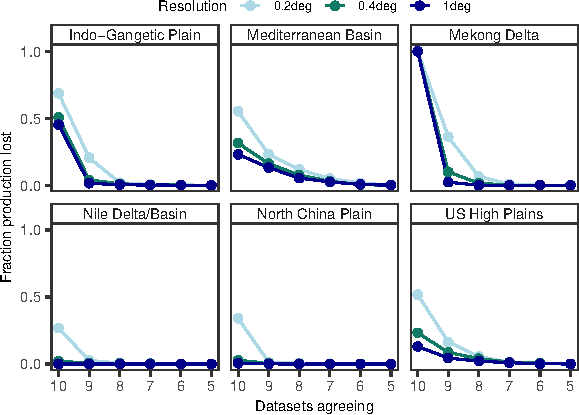
\includegraphics[keepaspectratio]{code_detectability_irrigated_areas_files/figure-latex/global_breadbaskets-1.pdf}}

\begin{Shaded}
\begin{Highlighting}[]
\CommentTok{\# MERGE \#\#\#\#\#\#\#\#\#\#\#\#\#\#\#\#\#\#\#\#\#\#\#\#\#\#\#\#\#\#\#\#\#\#\#\#\#\#\#\#\#\#\#\#\#\#\#\#\#\#\#\#\#\#\#\#\#\#\#\#\#\#\#\#\#\#\#\#\#\#\#\#}

\FunctionTok{plot\_grid}\NormalTok{(plot\_heatmap, plot\_fraction\_lost, }\AttributeTok{ncol =} \DecValTok{1}\NormalTok{, }\AttributeTok{labels =} \StringTok{"auto"}\NormalTok{, }\AttributeTok{rel\_heights =} \FunctionTok{c}\NormalTok{(}\FloatTok{0.55}\NormalTok{, }\FloatTok{0.45}\NormalTok{))}
\end{Highlighting}
\end{Shaded}

\pandocbounded{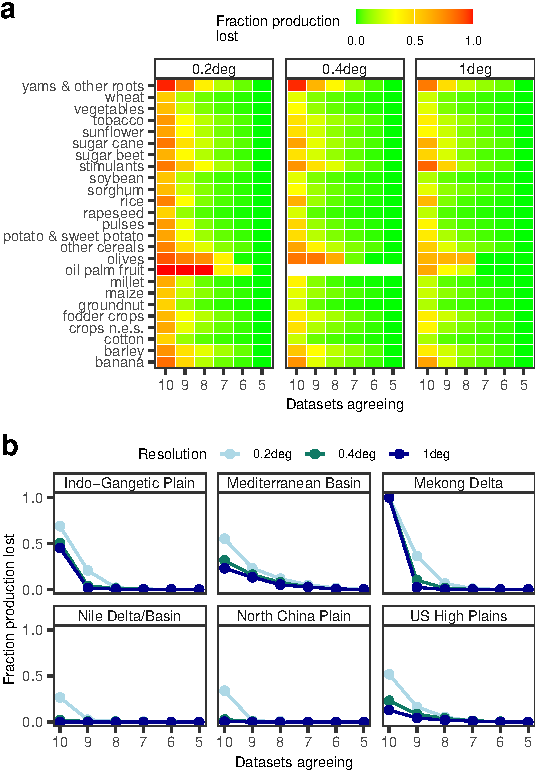
\includegraphics[keepaspectratio]{code_detectability_irrigated_areas_files/figure-latex/merge_crop_breadbasket-1.pdf}}

\begin{Shaded}
\begin{Highlighting}[]
\CommentTok{\# MERGE \#\#\#\#\#\#\#\#\#\#\#\#\#\#\#\#\#\#\#\#\#\#\#\#\#\#\#\#\#\#\#\#\#\#\#\#\#\#\#\#\#\#\#\#\#\#\#\#\#\#\#\#\#\#\#\#\#\#\#\#\#\#\#\#\#\#\#\#\#\#\#\#}

\NormalTok{plot\_fraction\_lost }\OtherTok{\textless{}{-}}\NormalTok{ plot\_fraction\_lost }\SpecialCharTok{+} 
  \FunctionTok{facet\_wrap}\NormalTok{(}\SpecialCharTok{\textasciitilde{}}\NormalTok{region, }\AttributeTok{ncol =} \DecValTok{2}\NormalTok{)}

\NormalTok{top }\OtherTok{\textless{}{-}} \FunctionTok{plot\_grid}\NormalTok{(plot\_heatmap, plot\_fraction\_lost, }\AttributeTok{ncol =} \DecValTok{2}\NormalTok{, }\AttributeTok{labels =} \StringTok{"auto"}\NormalTok{, }
                 \AttributeTok{rel\_widths =}  \FunctionTok{c}\NormalTok{(}\FloatTok{0.55}\NormalTok{, }\FloatTok{0.45}\NormalTok{))}

\NormalTok{top}
\end{Highlighting}
\end{Shaded}

\pandocbounded{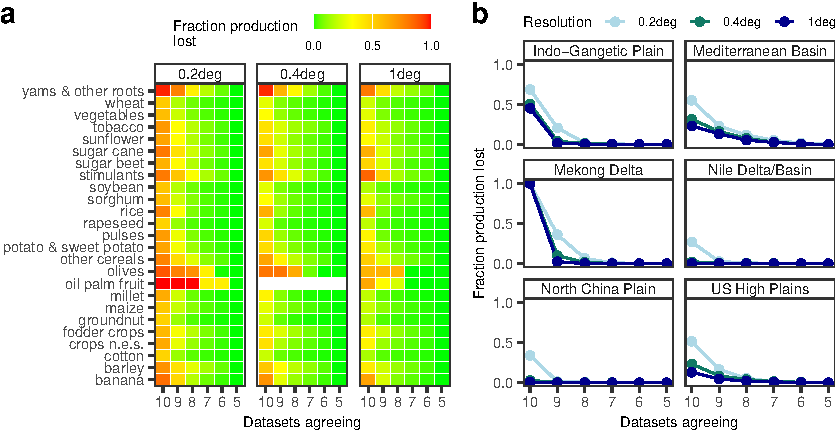
\includegraphics[keepaspectratio]{code_detectability_irrigated_areas_files/figure-latex/merge_crop_breadbasket2-1.pdf}}

\subsection{Irrigation-induced
evapotranspiration}\label{irrigation-induced-evapotranspiration}

\begin{Shaded}
\begin{Highlighting}[]
\CommentTok{\# LOAD THE HARMONIZED GRIDS \#\#\#\#\#\#\#\#\#\#\#\#\#\#\#\#\#\#\#\#\#\#\#\#\#\#\#\#\#\#\#\#\#\#\#\#\#\#\#\#\#\#\#\#\#\#\#\#\#\#\#\#}

\NormalTok{tmpl\_02 }\OtherTok{\textless{}{-}} \FunctionTok{rast}\NormalTok{(}\StringTok{"./mha\_stack\_ll\_02\_aligned\_NEAR.tif"}\NormalTok{)[[}\DecValTok{1}\NormalTok{]]}
\NormalTok{tmpl\_04 }\OtherTok{\textless{}{-}} \FunctionTok{rast}\NormalTok{(}\StringTok{"./mha\_stack\_ll\_04\_aligned\_NEAR.tif"}\NormalTok{)[[}\DecValTok{1}\NormalTok{]]}
\NormalTok{tmpl\_1 }\OtherTok{\textless{}{-}} \FunctionTok{rast}\NormalTok{(}\StringTok{"./mha\_stack\_ll\_10\_aligned\_NEAR.tif"}\NormalTok{)[[}\DecValTok{1}\NormalTok{]]}

\NormalTok{templates }\OtherTok{\textless{}{-}} \FunctionTok{list}\NormalTok{(}\StringTok{"0.2deg"} \OtherTok{=}\NormalTok{ tmpl\_02, }\StringTok{"0.4deg"} \OtherTok{=}\NormalTok{ tmpl\_04, }\StringTok{"1deg"} \OtherTok{=}\NormalTok{ tmpl\_1)}

\CommentTok{\# Enforce lon/lat WGS84 on templates if needed{-}{-}{-}{-}{-}{-}{-}{-}{-}{-}{-}{-}{-}{-}{-}{-}{-}{-}{-}{-}{-}{-}{-}{-}{-}{-}{-}{-}{-}{-}{-}{-}{-}{-}}

\NormalTok{templates }\OtherTok{\textless{}{-}} \FunctionTok{lapply}\NormalTok{(templates, }\ControlFlowTok{function}\NormalTok{(t) \{}
  \ControlFlowTok{if}\NormalTok{ (}\FunctionTok{is.na}\NormalTok{(}\FunctionTok{crs}\NormalTok{(t)) }\SpecialCharTok{||} \FunctionTok{crs}\NormalTok{(t) }\SpecialCharTok{==} \StringTok{""}\NormalTok{) }\FunctionTok{crs}\NormalTok{(t) }\OtherTok{\textless{}{-}} \StringTok{"EPSG:4326"}
\NormalTok{  t}
\NormalTok{\})}

\CommentTok{\# LOAD THE FILES \#\#\#\#\#\#\#\#\#\#\#\#\#\#\#\#\#\#\#\#\#\#\#\#\#\#\#\#\#\#\#\#\#\#\#\#\#\#\#\#\#\#\#\#\#\#\#\#\#\#\#\#\#\#\#\#\#\#\#\#\#\#\#}
\CommentTok{\# Files come from the Yao et al 2025 paper (Nature Water)}

\CommentTok{\# Year window {-}{-}{-}{-}{-}{-}{-}{-}{-}{-}{-}{-}{-}{-}{-}{-}{-}{-}{-}{-}{-}{-}{-}{-}{-}{-}{-}{-}{-}{-}{-}{-}{-}{-}{-}{-}{-}{-}{-}{-}{-}{-}{-}{-}{-}{-}{-}{-}{-}{-}{-}{-}{-}{-}{-}{-}{-}{-}{-}{-}{-}{-}{-}{-}{-}{-}}

\NormalTok{win }\OtherTok{\textless{}{-}} \StringTok{"1985\_2014\_timmean"}

\CommentTok{\# Base directory {-}{-}{-}{-}{-}{-}{-}{-}{-}{-}{-}{-}{-}{-}{-}{-}{-}{-}{-}{-}{-}{-}{-}{-}{-}{-}{-}{-}{-}{-}{-}{-}{-}{-}{-}{-}{-}{-}{-}{-}{-}{-}{-}{-}{-}{-}{-}{-}{-}{-}{-}{-}{-}{-}{-}{-}{-}{-}{-}{-}{-}{-}{-}}

\NormalTok{base\_dir }\OtherTok{\textless{}{-}} \StringTok{"./yao\_et\_al\_2025\_datasets/water\_fluxes/CESM2"}

\CommentTok{\# Paste {-}{-}{-}{-}{-}{-}{-}{-}{-}{-}{-}{-}{-}{-}{-}{-}{-}{-}{-}{-}{-}{-}{-}{-}{-}{-}{-}{-}{-}{-}{-}{-}{-}{-}{-}{-}{-}{-}{-}{-}{-}{-}{-}{-}{-}{-}{-}{-}{-}{-}{-}{-}{-}{-}{-}{-}{-}{-}{-}{-}{-}{-}{-}{-}{-}{-}{-}{-}{-}{-}{-}{-}}

\NormalTok{irr\_files }\OtherTok{\textless{}{-}} \FunctionTok{paste0}\NormalTok{(base\_dir, }\StringTok{"/CESM2\_IRR0"}\NormalTok{, }\DecValTok{1}\SpecialCharTok{:}\DecValTok{3}\NormalTok{, }\StringTok{"\_1901\_2014\_QFLX\_EVAP\_TOT\_yearmean\_"}\NormalTok{, win)}
\NormalTok{noi\_files }\OtherTok{\textless{}{-}} \FunctionTok{paste0}\NormalTok{(base\_dir, }\StringTok{"/CESM2\_NOI0"}\NormalTok{, }\DecValTok{1}\SpecialCharTok{:}\DecValTok{3}\NormalTok{, }\StringTok{"\_1901\_2014\_QFLX\_EVAP\_TOT\_yearmean\_"}\NormalTok{, win)}

\CommentTok{\# BUILD ET STACKS + ENSEMBLE MEAN PER RESOLUTION \#\#\#\#\#\#\#\#\#\#\#\#\#\#\#\#\#\#\#\#\#\#\#\#\#\#\#\#\#\#\#\#}

\NormalTok{d\_list }\OtherTok{\textless{}{-}} \FunctionTok{Map}\NormalTok{(}\ControlFlowTok{function}\NormalTok{(irr\_f, noi\_f) }\FunctionTok{delta\_pair\_resampled}\NormalTok{(irr\_f, noi\_f, templates),}
\NormalTok{              irr\_files, noi\_files)}

\CommentTok{\# d\_list length 3; each element is list("0.2deg"=rast, "0.4deg"=rast, "1deg"=rast)}
\NormalTok{dET\_mean\_rasters }\OtherTok{\textless{}{-}} \FunctionTok{lapply}\NormalTok{(}\FunctionTok{names}\NormalTok{(templates), }\ControlFlowTok{function}\NormalTok{(res\_name) \{}

\NormalTok{  d\_rasters }\OtherTok{\textless{}{-}} \FunctionTok{lapply}\NormalTok{(d\_list, }\ControlFlowTok{function}\NormalTok{(one\_pair) one\_pair[[res\_name]])}
\NormalTok{  s }\OtherTok{\textless{}{-}}\NormalTok{ terra}\SpecialCharTok{::}\FunctionTok{rast}\NormalTok{(d\_rasters) }\CommentTok{\# 3{-}layer stack}
  \FunctionTok{names}\NormalTok{(s) }\OtherTok{\textless{}{-}} \FunctionTok{paste0}\NormalTok{(}\StringTok{"dET\_IRR0"}\NormalTok{, }\DecValTok{1}\SpecialCharTok{:}\DecValTok{3}\NormalTok{, }\StringTok{"\_mmday"}\NormalTok{)}

  \CommentTok{\# ensemble mean: cell{-}by{-}cell mean across 3 members}
\NormalTok{  m }\OtherTok{\textless{}{-}}\NormalTok{ terra}\SpecialCharTok{::}\FunctionTok{app}\NormalTok{(s, }\AttributeTok{fun =}\NormalTok{ mean, }\AttributeTok{na.rm =} \ConstantTok{TRUE}\NormalTok{)}
  \FunctionTok{names}\NormalTok{(m) }\OtherTok{\textless{}{-}} \FunctionTok{paste0}\NormalTok{(}\StringTok{"CESM2\_dET\_mean\_"}\NormalTok{, win, }\StringTok{"\_"}\NormalTok{, res\_name, }\StringTok{"\_mmday"}\NormalTok{)}

  \FunctionTok{list}\NormalTok{(}\AttributeTok{stack =}\NormalTok{ s, }\AttributeTok{mean =}\NormalTok{ m)}
\NormalTok{\})}
\FunctionTok{names}\NormalTok{(dET\_mean\_rasters) }\OtherTok{\textless{}{-}} \FunctionTok{names}\NormalTok{(templates)}

\CommentTok{\# EXPORT TO DATA TABLE \#\#\#\#\#\#\#\#\#\#\#\#\#\#\#\#\#\#\#\#\#\#\#\#\#\#\#\#\#\#\#\#\#\#\#\#\#\#\#\#\#\#\#\#\#\#\#\#\#\#\#\#\#\#\#\#\#}

\NormalTok{dET\_dt }\OtherTok{\textless{}{-}} \FunctionTok{lapply}\NormalTok{(}\FunctionTok{names}\NormalTok{(templates), }\ControlFlowTok{function}\NormalTok{(res\_name) \{}
\NormalTok{  tmpl }\OtherTok{\textless{}{-}}\NormalTok{ templates[[res\_name]]}
\NormalTok{  out }\OtherTok{\textless{}{-}}\NormalTok{ dET\_mean\_rasters[[res\_name]]}

\NormalTok{  dt\_mean }\OtherTok{\textless{}{-}} \FunctionTok{rast\_to\_dt\_with\_cell}\NormalTok{(out}\SpecialCharTok{$}\NormalTok{mean, tmpl, }\AttributeTok{value\_name =} \StringTok{"dET\_mean\_mmday"}\NormalTok{)}
\NormalTok{  dt\_mean[, resolution}\SpecialCharTok{:=}\NormalTok{ res\_name]}

\NormalTok{  dt\_members }\OtherTok{\textless{}{-}} \FunctionTok{rbindlist}\NormalTok{(}\FunctionTok{lapply}\NormalTok{(}\DecValTok{1}\SpecialCharTok{:}\NormalTok{terra}\SpecialCharTok{::}\FunctionTok{nlyr}\NormalTok{(out}\SpecialCharTok{$}\NormalTok{stack), }\ControlFlowTok{function}\NormalTok{(i) \{}
\NormalTok{    rr }\OtherTok{\textless{}{-}}\NormalTok{ out}\SpecialCharTok{$}\NormalTok{stack[[i]]}
\NormalTok{    dt }\OtherTok{\textless{}{-}} \FunctionTok{rast\_to\_dt\_with\_cell}\NormalTok{(rr, tmpl, }\AttributeTok{value\_name =} \StringTok{"dET\_mmday"}\NormalTok{)}
\NormalTok{    dt[, member}\SpecialCharTok{:=} \FunctionTok{names}\NormalTok{(rr)] }\CommentTok{\# dET\_IRR01\_mmday / dET\_IRR02\_mmday / dET\_IRR03\_mmday}
\NormalTok{    dt[, resolution}\SpecialCharTok{:=}\NormalTok{ res\_name]}
\NormalTok{    dt[]}
\NormalTok{  \}))}

  \FunctionTok{list}\NormalTok{(}\AttributeTok{mean =}\NormalTok{ dt\_mean, }\AttributeTok{members =}\NormalTok{ dt\_members)}
\NormalTok{\})}
\FunctionTok{names}\NormalTok{(dET\_dt) }\OtherTok{\textless{}{-}} \FunctionTok{names}\NormalTok{(templates)}

\CommentTok{\# COMPUTE K{-}OF{-}10 AGREEMENT WITH CELL JOINS \#\#\#\#\#\#\#\#\#\#\#\#\#\#\#\#\#\#\#\#\#\#\#\#\#\#\#\#\#\#\#\#\#\#\#\#}

\NormalTok{resolutions }\OtherTok{\textless{}{-}} \FunctionTok{c}\NormalTok{(}\StringTok{"0.2deg"}\NormalTok{, }\StringTok{"0.4deg"}\NormalTok{, }\StringTok{"1deg"}\NormalTok{)}
\NormalTok{ks }\OtherTok{\textless{}{-}} \DecValTok{5}\SpecialCharTok{:}\DecValTok{10}

\CommentTok{\# Compute {-}{-}{-}{-}{-}{-}{-}{-}{-}{-}{-}{-}{-}{-}{-}{-}{-}{-}{-}{-}{-}{-}{-}{-}{-}{-}{-}{-}{-}{-}{-}{-}{-}{-}{-}{-}{-}{-}{-}{-}{-}{-}{-}{-}{-}{-}{-}{-}{-}{-}{-}{-}{-}{-}{-}{-}{-}{-}{-}{-}{-}{-}{-}{-}{-}{-}{-}{-}{-}{-}}

\NormalTok{out\_k\_all }\OtherTok{\textless{}{-}} \FunctionTok{rbindlist}\NormalTok{(}\FunctionTok{lapply}\NormalTok{(resolutions, }\ControlFlowTok{function}\NormalTok{(res) \{}

\NormalTok{  tmpl }\OtherTok{\textless{}{-}}\NormalTok{ templates[[res]]}

  \CommentTok{\# irrigation presence{-}{-}{-}{-}{-}{-}{-}{-}{-}{-}{-}{-}{-}}

\NormalTok{  dt\_irrig\_raw }\OtherTok{\textless{}{-}} \FunctionTok{copy}\NormalTok{(dt\_pres)[resolution }\SpecialCharTok{==}\NormalTok{ res]}
\NormalTok{  dt\_irrig }\OtherTok{\textless{}{-}} \FunctionTok{pres\_to\_cell}\NormalTok{(dt\_irrig\_raw, tmpl)}

  \CommentTok{\# add cell area{-}{-}{-}{-}{-}{-}{-}{-}{-}{-}{-}{-}{-}{-}{-}{-}{-}{-}}

\NormalTok{  dt\_area }\OtherTok{\textless{}{-}} \FunctionTok{cell\_area\_dt}\NormalTok{(tmpl)}
  \FunctionTok{setkey}\NormalTok{(dt\_irrig, cell)}
  \FunctionTok{setkey}\NormalTok{(dt\_area,  cell)}
\NormalTok{  dt\_irrig }\OtherTok{\textless{}{-}}\NormalTok{ dt\_irrig[dt\_area]  }\CommentTok{\# add area\_m2}

  \CommentTok{\# increase ET mean table {-}{-}{-}{-}{-}{-}{-}{-}{-}{-}}

\NormalTok{  dt\_et }\OtherTok{\textless{}{-}} \FunctionTok{copy}\NormalTok{(dET\_dt[[res]]}\SpecialCharTok{$}\NormalTok{mean)}
\NormalTok{  valcol }\OtherTok{\textless{}{-}} \FunctionTok{setdiff}\NormalTok{(}\FunctionTok{names}\NormalTok{(dt\_et), }\FunctionTok{c}\NormalTok{(}\StringTok{"cell"}\NormalTok{,}\StringTok{"lon"}\NormalTok{,}\StringTok{"lat"}\NormalTok{,}\StringTok{"resolution"}\NormalTok{))[}\DecValTok{1}\NormalTok{]}

  \CommentTok{\# Join: we keep all ET cells and bring irrigation info when available:}
  \CommentTok{\# to summarise ONLY cells that exist in the irrigation table:}
  \CommentTok{\#   dt\_join \textless{}{-} dt\_et[dt\_irrig, on="cell"]}
  \FunctionTok{setkey}\NormalTok{(dt\_et, cell)}
\NormalTok{  dt\_join }\OtherTok{\textless{}{-}}\NormalTok{ dt\_irrig[dt\_et]}

  \FunctionTok{rbindlist}\NormalTok{(}\FunctionTok{lapply}\NormalTok{(ks, }\ControlFlowTok{function}\NormalTok{(k) \{}

\NormalTok{    dt\_sub }\OtherTok{\textless{}{-}}\NormalTok{ dt\_join[n\_pos }\SpecialCharTok{\textgreater{}=}\NormalTok{ k]}

    \CommentTok{\# restrict weights to cells with non{-}missing ET and non{-}missing area}
\NormalTok{    ok }\OtherTok{\textless{}{-}} \SpecialCharTok{!}\FunctionTok{is.na}\NormalTok{(dt\_sub[[valcol]]) }\SpecialCharTok{\&} \SpecialCharTok{!}\FunctionTok{is.na}\NormalTok{(dt\_sub}\SpecialCharTok{$}\NormalTok{area\_m2)}
\NormalTok{    w  }\OtherTok{\textless{}{-}}\NormalTok{ dt\_sub}\SpecialCharTok{$}\NormalTok{area\_m2[ok]}
\NormalTok{    x  }\OtherTok{\textless{}{-}}\NormalTok{ dt\_sub[[valcol]][ok]}

    \CommentTok{\# area{-}weighted mean increase ET (mm/day)}
\NormalTok{    mean\_aw }\OtherTok{\textless{}{-}} \ControlFlowTok{if}\NormalTok{ (}\FunctionTok{length}\NormalTok{(x) }\SpecialCharTok{==} \DecValTok{0}\DataTypeTok{L}\NormalTok{) }\ConstantTok{NA\_real\_} \ControlFlowTok{else} \FunctionTok{sum}\NormalTok{(x }\SpecialCharTok{*}\NormalTok{ w) }\SpecialCharTok{/} \FunctionTok{sum}\NormalTok{(w)}

    \CommentTok{\# area{-}weighted aggregate: mm/day * m\^{}2 {-}\textgreater{} m\^{}3/day}
    \CommentTok{\# 1 mm = 0.001 m}
\NormalTok{    sum\_m3day }\OtherTok{\textless{}{-}} \ControlFlowTok{if}\NormalTok{ (}\FunctionTok{length}\NormalTok{(x) }\SpecialCharTok{==} \DecValTok{0}\DataTypeTok{L}\NormalTok{) }\ConstantTok{NA\_real\_} \ControlFlowTok{else} \FunctionTok{sum}\NormalTok{(x }\SpecialCharTok{*}\NormalTok{ w) }\SpecialCharTok{*} \FloatTok{1e{-}3}

    \FunctionTok{data.table}\NormalTok{(}\AttributeTok{resolution =}\NormalTok{ res,}
               \AttributeTok{k =}\NormalTok{ k,}
               \AttributeTok{n\_cells\_irrig\_k =} \FunctionTok{sum}\NormalTok{(dt\_irrig}\SpecialCharTok{$}\NormalTok{n\_pos }\SpecialCharTok{\textgreater{}=}\NormalTok{ k, }\AttributeTok{na.rm =} \ConstantTok{TRUE}\NormalTok{),}
               \AttributeTok{n\_cells\_join\_k =} \FunctionTok{nrow}\NormalTok{(dt\_sub),}
               \AttributeTok{n\_cells\_with\_dET\_k =} \FunctionTok{sum}\NormalTok{(}\SpecialCharTok{!}\FunctionTok{is.na}\NormalTok{(dt\_sub[[valcol]])),}
               \AttributeTok{mean\_dET\_mmday =} \FunctionTok{mean}\NormalTok{(dt\_sub[[valcol]], }\AttributeTok{na.rm =} \ConstantTok{TRUE}\NormalTok{),}
               \AttributeTok{sum\_dET\_mmday\_unweighted =} \FunctionTok{sum}\NormalTok{(dt\_sub[[valcol]], }\AttributeTok{na.rm =} \ConstantTok{TRUE}\NormalTok{),}
               \AttributeTok{mean\_dET\_mmday\_areaweighted =}\NormalTok{ mean\_aw,}
               \AttributeTok{sum\_dET\_m3day\_areaweighted =}\NormalTok{ sum\_m3day,}
               \AttributeTok{area\_m2\_with\_dET\_k =} \ControlFlowTok{if}\NormalTok{ (}\FunctionTok{length}\NormalTok{(w) }\SpecialCharTok{==} \DecValTok{0}\DataTypeTok{L}\NormalTok{) }\DecValTok{0} \ControlFlowTok{else} \FunctionTok{sum}\NormalTok{(w)}
\NormalTok{    )}
\NormalTok{  \}))}
\NormalTok{\}))}

\NormalTok{out\_k\_all}
\end{Highlighting}
\end{Shaded}

\begin{verbatim}
##     resolution     k n_cells_irrig_k n_cells_join_k n_cells_with_dET_k
##         <char> <int>           <int>          <int>              <int>
##  1:     0.2deg     5           46644          46644              46451
##  2:     0.2deg     6           41944          41944              41801
##  3:     0.2deg     7           35938          35938              35827
##  4:     0.2deg     8           28101          28101              28031
##  5:     0.2deg     9           18390          18390              18360
##  6:     0.2deg    10            7304           7304               7291
##  7:     0.4deg     5           14324          14324              14268
##  8:     0.4deg     6           13177          13177              13130
##  9:     0.4deg     7           11614          11614              11575
## 10:     0.4deg     8            9669           9669               9641
## 11:     0.4deg     9            7295           7295               7282
## 12:     0.4deg    10            4001           4001               3997
## 13:       1deg     5            2811           2811               2806
## 14:       1deg     6            2607           2607               2602
## 15:       1deg     7            2385           2385               2381
## 16:       1deg     8            2108           2108               2104
## 17:       1deg     9            1707           1707               1706
## 18:       1deg    10            1048           1048               1048
##     mean_dET_mmday sum_dET_mmday_unweighted mean_dET_mmday_areaweighted
##              <num>                    <num>                       <num>
##  1:     0.04028864               1871.44764                  0.04029326
##  2:     0.04357686               1821.55644                  0.04365208
##  3:     0.04879833               1748.29771                  0.04897260
##  4:     0.05774762               1618.72349                  0.05813341
##  5:     0.07212178               1324.15586                  0.07297354
##  6:     0.08834509                644.12404                  0.09012513
##  7:     0.03687360                526.11255                  0.03676943
##  8:     0.03938979                517.18794                  0.03932189
##  9:     0.04324888                500.60583                  0.04325003
## 10:     0.04940505                476.31404                  0.04953749
## 11:     0.05956280                433.73629                  0.06005056
## 12:     0.07746101                309.61167                  0.07885857
## 13:     0.03348482                 93.95841                  0.03327423
## 14:     0.03583793                 93.25030                  0.03567600
## 15:     0.03862680                 91.97040                  0.03850129
## 16:     0.04270399                 89.84920                  0.04263743
## 17:     0.04940630                 84.28715                  0.04957431
## 18:     0.06332167                 66.36111                  0.06431951
##     sum_dET_m3day_areaweighted area_m2_with_dET_k
##                          <num>              <num>
##  1:                  778776266       1.932771e+13
##  2:                  759169818       1.739138e+13
##  3:                  730098982       1.490831e+13
##  4:                  677583129       1.165566e+13
##  5:                  554023695       7.592118e+12
##  6:                  267435074       2.967375e+12
##  7:                  871863692       2.371165e+13
##  8:                  858139152       2.182345e+13
##  9:                  832376294       1.924568e+13
## 10:                  793535217       1.601888e+13
## 11:                  724704062       1.206823e+13
## 12:                  512997489       6.505285e+12
## 13:                  967432320       2.907452e+13
## 14:                  961166448       2.694154e+13
## 15:                  949967797       2.467366e+13
## 16:                  929444480       2.179879e+13
## 17:                  874062929       1.763137e+13
## 18:                  683352218       1.062434e+13
\end{verbatim}

\begin{Shaded}
\begin{Highlighting}[]
\CommentTok{\# PLOT \#\#\#\#\#\#\#\#\#\#\#\#\#\#\#\#\#\#\#\#\#\#\#\#\#\#\#\#\#\#\#\#\#\#\#\#\#\#\#\#\#\#\#\#\#\#\#\#\#\#\#\#\#\#\#\#\#\#\#\#\#\#\#\#\#\#\#\#\#\#\#\#\#}

\CommentTok{\# Condition ifesle {-}{-}{-}{-}{-}{-}{-}{-}{-}{-}{-}{-}{-}{-}{-}{-}{-}{-}{-}{-}{-}{-}{-}{-}{-}{-}{-}{-}{-}{-}{-}{-}{-}{-}{-}{-}{-}{-}{-}{-}{-}{-}{-}{-}{-}{-}{-}{-}{-}{-}{-}{-}{-}{-}{-}{-}{-}{-}{-}{-}{-}}

\NormalTok{total\_col }\OtherTok{\textless{}{-}} \ControlFlowTok{if}\NormalTok{ (}\StringTok{"sum\_dET\_m3day\_areaweighted"} \SpecialCharTok{\%in\%} \FunctionTok{names}\NormalTok{(out\_k\_all)) \{}
  \StringTok{"sum\_dET\_m3day\_areaweighted"}
\NormalTok{\} }\ControlFlowTok{else} \ControlFlowTok{if}\NormalTok{ (}\StringTok{"sum\_dET\_mmday\_unweighted"} \SpecialCharTok{\%in\%} \FunctionTok{names}\NormalTok{(out\_k\_all)) \{}
  \StringTok{"sum\_dET\_mmday\_unweighted"}
\NormalTok{\} }\ControlFlowTok{else}\NormalTok{ \{}
  \FunctionTok{stop}\NormalTok{(}\StringTok{"out\_k\_all has neither sum\_dET\_m3day\_areaweighted nor sum\_dET\_mmday\_unweighted"}\NormalTok{)}
\NormalTok{\}}

\CommentTok{\# Convert m3/day to km3/day {-}{-}{-}{-}{-}{-}{-}{-}{-}{-}{-}{-}{-}{-}{-}{-}{-}{-}{-}{-}{-}{-}{-}{-}{-}{-}{-}{-}{-}{-}{-}{-}{-}{-}{-}{-}{-}{-}{-}{-}{-}{-}{-}{-}{-}{-}{-}{-}{-}{-}{-}{-}}

\NormalTok{out\_plot }\OtherTok{\textless{}{-}} \FunctionTok{copy}\NormalTok{(out\_k\_all)}

\ControlFlowTok{if}\NormalTok{ (total\_col }\SpecialCharTok{==} \StringTok{"sum\_dET\_m3day\_areaweighted"}\NormalTok{) \{}
\NormalTok{  out\_plot[, total\_km3day }\SpecialCharTok{:=} \FunctionTok{get}\NormalTok{(total\_col) }\SpecialCharTok{/} \FloatTok{1e9}\NormalTok{]}
\NormalTok{  total\_ylab }\OtherTok{\textless{}{-}} \StringTok{"Total irrigation{-}}\SpecialCharTok{\textbackslash{}n}\StringTok{induced ET (km³ d{-}¹)"}

\NormalTok{\} }\ControlFlowTok{else}\NormalTok{ \{}

\NormalTok{  out\_plot[, total\_km3day }\SpecialCharTok{:=} \FunctionTok{get}\NormalTok{(total\_col)]}
\NormalTok{  total\_ylab }\OtherTok{\textless{}{-}} \StringTok{"Total irrigation{-}induced }\SpecialCharTok{\textbackslash{}n}\StringTok{ET signal (sum of mm/day)"}
\NormalTok{\}}

\CommentTok{\# Keep only k = 5, ..., 10{-}{-}{-}{-}{-}{-}{-}{-}{-}{-}{-}{-}{-}{-}{-}{-}{-}{-}{-}{-}{-}{-}{-}{-}{-}{-}{-}{-}{-}{-}{-}{-}{-}{-}{-}{-}{-}{-}{-}{-}{-}{-}{-}{-}{-}{-}{-}{-}{-}{-}{-}{-}{-}{-}}

\NormalTok{out\_plot }\OtherTok{\textless{}{-}}\NormalTok{ out\_plot[k }\SpecialCharTok{\%in\%} \DecValTok{5}\SpecialCharTok{:}\DecValTok{10}\NormalTok{]}

\CommentTok{\# Plot mean increase in irrigation{-}induced ET {-}{-}{-}{-}{-}{-}{-}{-}{-}{-}{-}{-}{-}{-}{-}{-}{-}{-}{-}{-}{-}{-}{-}{-}{-}{-}{-}{-}{-}{-}{-}{-}{-}{-}}
\CommentTok{\# (average irrigation{-}induced evapotranspiration change per grid cell)}

\NormalTok{plot\_mean\_ET }\OtherTok{\textless{}{-}} \FunctionTok{ggplot}\NormalTok{(out\_plot, }\FunctionTok{aes}\NormalTok{(k, mean\_dET\_mmday, }\AttributeTok{colour =}\NormalTok{ resolution,}
                                     \AttributeTok{group =}\NormalTok{ resolution)) }\SpecialCharTok{+}
  \FunctionTok{geom\_line}\NormalTok{() }\SpecialCharTok{+}
  \FunctionTok{geom\_point}\NormalTok{() }\SpecialCharTok{+}
  \FunctionTok{labs}\NormalTok{(}\AttributeTok{x =} \StringTok{"Datasets agreeing"}\NormalTok{, }
       \AttributeTok{y =} \FunctionTok{expression}\NormalTok{(}\FunctionTok{atop}\NormalTok{(}\StringTok{"Mean "} \SpecialCharTok{*}\NormalTok{ Delta }\SpecialCharTok{*}\NormalTok{ ET[irr], }\StringTok{"(mm d"}\SpecialCharTok{\^{}}\NormalTok{\{}\SpecialCharTok{{-}}\DecValTok{1}\NormalTok{\} }\SpecialCharTok{*} \StringTok{")"}\NormalTok{))) }\SpecialCharTok{+}
  \FunctionTok{scale\_x\_reverse}\NormalTok{(}\AttributeTok{breaks =} \DecValTok{10}\SpecialCharTok{:}\DecValTok{5}\NormalTok{) }\SpecialCharTok{+}
  \FunctionTok{scale\_color\_manual}\NormalTok{(}\AttributeTok{values =}\NormalTok{ res\_palette) }\SpecialCharTok{+}
  \FunctionTok{theme\_AP}\NormalTok{() }\SpecialCharTok{+}
  \FunctionTok{theme}\NormalTok{(}\AttributeTok{legend.position =} \StringTok{"none"}\NormalTok{)}

\CommentTok{\# Plot total irrigation induced ET {-}{-}{-}{-}{-}{-}{-}{-}{-}{-}{-}{-}{-}{-}{-}{-}{-}{-}{-}{-}{-}{-}{-}{-}{-}{-}{-}{-}{-}{-}{-}{-}{-}{-}{-}{-}{-}{-}{-}{-}{-}{-}{-}{-}{-}}
\CommentTok{\# (global irrigation{-}induced evapotranspiration signal, obtained by integrating}
\CommentTok{\# over all retained cells; e.g., total amount of water transferred to the }
\CommentTok{\# atmosphere per day because of irrigation)}

\NormalTok{plot\_total\_ET }\OtherTok{\textless{}{-}} \FunctionTok{ggplot}\NormalTok{(out\_plot, }\FunctionTok{aes}\NormalTok{(k, total\_km3day, }\AttributeTok{colour =}\NormalTok{ resolution, }\AttributeTok{group =}\NormalTok{ resolution)) }\SpecialCharTok{+}
  \FunctionTok{geom\_line}\NormalTok{() }\SpecialCharTok{+}
  \FunctionTok{geom\_point}\NormalTok{() }\SpecialCharTok{+}
  \FunctionTok{labs}\NormalTok{(}\AttributeTok{x =} \StringTok{"Datasets agreeing"}\NormalTok{, }\AttributeTok{y =}\NormalTok{ total\_ylab) }\SpecialCharTok{+}
  \FunctionTok{scale\_x\_reverse}\NormalTok{(}\AttributeTok{breaks =} \DecValTok{10}\SpecialCharTok{:}\DecValTok{5}\NormalTok{) }\SpecialCharTok{+}
  \FunctionTok{scale\_color\_manual}\NormalTok{(}\AttributeTok{values =}\NormalTok{ res\_palette) }\SpecialCharTok{+}
  \FunctionTok{theme\_AP}\NormalTok{() }\SpecialCharTok{+}
  \FunctionTok{theme}\NormalTok{(}\AttributeTok{legend.position =} \StringTok{"none"}\NormalTok{)}

\CommentTok{\# Plot area with irrigation{-}induced ET retained under k{-}{-}{-}{-}{-}{-}{-}{-}{-}{-}{-}{-}{-}{-}{-}{-}{-}{-}{-}{-}{-}{-}{-}{-}{-}}

\NormalTok{out\_plot }\OtherTok{\textless{}{-}} \FunctionTok{copy}\NormalTok{(out\_k\_all)[k }\SpecialCharTok{\%in\%} \DecValTok{5}\SpecialCharTok{:}\DecValTok{10}\NormalTok{]}

\CommentTok{\# convert m2 to Mha {-}{-}{-}{-}{-}{-}{-}{-}{-}{-}{-}{-}{-}{-}{-}{-}{-}{-}{-}{-}{-}{-}{-}{-}{-}{-}{-}{-}{-}{-}{-}{-}{-}{-}{-}}
\NormalTok{out\_plot[, area\_Mha}\SpecialCharTok{:=}\NormalTok{ area\_m2\_with\_dET\_k }\SpecialCharTok{/} \FloatTok{1e10}\NormalTok{]}

\CommentTok{\# also show contraction relative to k=5 within each resolution}
\NormalTok{out\_plot[, area\_frac\_vs\_k5}\SpecialCharTok{:=}\NormalTok{ area\_m2\_with\_dET\_k }\SpecialCharTok{/}\NormalTok{ area\_m2\_with\_dET\_k[k }\SpecialCharTok{==} \DecValTok{5}\NormalTok{], by }\OtherTok{=}\NormalTok{ resolution]}

\CommentTok{\# Total land area of grid cells with reported irrigated areas}
\NormalTok{plot\_area }\OtherTok{\textless{}{-}} \FunctionTok{ggplot}\NormalTok{(out\_plot, }\FunctionTok{aes}\NormalTok{(k, area\_Mha, }\AttributeTok{colour =}\NormalTok{ resolution, }\AttributeTok{group =}\NormalTok{ resolution)) }\SpecialCharTok{+}
  \FunctionTok{geom\_line}\NormalTok{() }\SpecialCharTok{+}
  \FunctionTok{geom\_point}\NormalTok{() }\SpecialCharTok{+}
  \FunctionTok{labs}\NormalTok{(}\AttributeTok{x =} \StringTok{"Datasets agreeing"}\NormalTok{, }\AttributeTok{y =} \StringTok{"Area irrigation }\SpecialCharTok{\textbackslash{}n}\StringTok{signal (Mha)"}\NormalTok{) }\SpecialCharTok{+}
  \FunctionTok{scale\_x\_reverse}\NormalTok{(}\AttributeTok{breaks =} \DecValTok{10}\SpecialCharTok{:}\DecValTok{5}\NormalTok{) }\SpecialCharTok{+}
  \FunctionTok{scale\_color\_manual}\NormalTok{(}\AttributeTok{values =}\NormalTok{ res\_palette) }\SpecialCharTok{+}
  \FunctionTok{theme\_AP}\NormalTok{() }\SpecialCharTok{+}
  \FunctionTok{theme}\NormalTok{(}\AttributeTok{legend.position =} \StringTok{"none"}\NormalTok{)}

\NormalTok{plot\_area}
\end{Highlighting}
\end{Shaded}

\pandocbounded{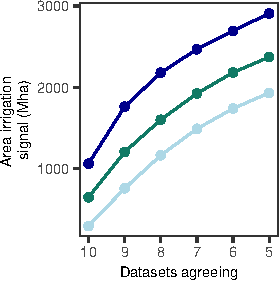
\includegraphics[keepaspectratio]{code_detectability_irrigated_areas_files/figure-latex/irrigation_ET-1.pdf}}

\begin{Shaded}
\begin{Highlighting}[]
\CommentTok{\# Also in case: fraction of area retained vs k=5}
\NormalTok{plot\_area\_fraction }\OtherTok{\textless{}{-}} \FunctionTok{ggplot}\NormalTok{(out\_plot, }\FunctionTok{aes}\NormalTok{(k, area\_frac\_vs\_k5, }\AttributeTok{colour =}\NormalTok{ resolution, }\AttributeTok{group =}\NormalTok{ resolution)) }\SpecialCharTok{+}
  \FunctionTok{geom\_hline}\NormalTok{(}\AttributeTok{yintercept =} \DecValTok{1}\NormalTok{, }\AttributeTok{linewidth =} \FloatTok{0.4}\NormalTok{) }\SpecialCharTok{+}
  \FunctionTok{geom\_line}\NormalTok{() }\SpecialCharTok{+}
  \FunctionTok{geom\_point}\NormalTok{() }\SpecialCharTok{+}
  \FunctionTok{labs}\NormalTok{(}\AttributeTok{x =} \StringTok{"Datasets agreeing"}\NormalTok{,}
       \AttributeTok{y =} \FunctionTok{expression}\NormalTok{(}\StringTok{"Area retaining "}\SpecialCharTok{\textasciitilde{}}\NormalTok{Delta}\SpecialCharTok{*}\NormalTok{ET}\SpecialCharTok{\textasciitilde{}}\StringTok{" (fraction of k=5)"}\NormalTok{)) }\SpecialCharTok{+}
  \FunctionTok{scale\_x\_reverse}\NormalTok{(}\AttributeTok{breaks =} \DecValTok{10}\SpecialCharTok{:}\DecValTok{5}\NormalTok{) }\SpecialCharTok{+}
  \FunctionTok{scale\_y\_continuous}\NormalTok{(}\AttributeTok{limits =} \FunctionTok{c}\NormalTok{(}\DecValTok{0}\NormalTok{, }\FloatTok{1.05}\NormalTok{)) }\SpecialCharTok{+}
  \FunctionTok{scale\_color\_manual}\NormalTok{(}\AttributeTok{values =}\NormalTok{ res\_palette) }\SpecialCharTok{+}
  \FunctionTok{theme\_AP}\NormalTok{() }\SpecialCharTok{+}
  \FunctionTok{theme}\NormalTok{(}\AttributeTok{legend.position =} \StringTok{"none"}\NormalTok{)}

\NormalTok{plot\_area\_fraction}
\end{Highlighting}
\end{Shaded}

\pandocbounded{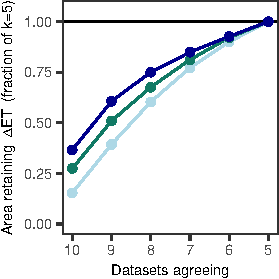
\includegraphics[keepaspectratio]{code_detectability_irrigated_areas_files/figure-latex/irrigation_ET-2.pdf}}

\begin{Shaded}
\begin{Highlighting}[]
\NormalTok{bottom }\OtherTok{\textless{}{-}} \FunctionTok{plot\_grid}\NormalTok{(plot\_mean\_ET, plot\_total\_ET, plot\_area, }\AttributeTok{labels =} \FunctionTok{c}\NormalTok{(}\StringTok{"c"}\NormalTok{, }\StringTok{"d"}\NormalTok{, }\StringTok{"e"}\NormalTok{),}
                    \AttributeTok{ncol =} \DecValTok{3}\NormalTok{)}
\NormalTok{bottom}
\end{Highlighting}
\end{Shaded}

\pandocbounded{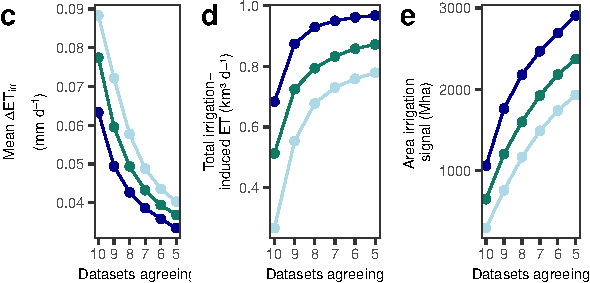
\includegraphics[keepaspectratio]{code_detectability_irrigated_areas_files/figure-latex/merge_ET_plots-1.pdf}}

\begin{Shaded}
\begin{Highlighting}[]
\FunctionTok{plot\_grid}\NormalTok{(top, bottom, }\AttributeTok{ncol =} \DecValTok{1}\NormalTok{, }\AttributeTok{rel\_heights =} \FunctionTok{c}\NormalTok{(}\FloatTok{0.685}\NormalTok{, }\FloatTok{0.325}\NormalTok{))}
\end{Highlighting}
\end{Shaded}

\pandocbounded{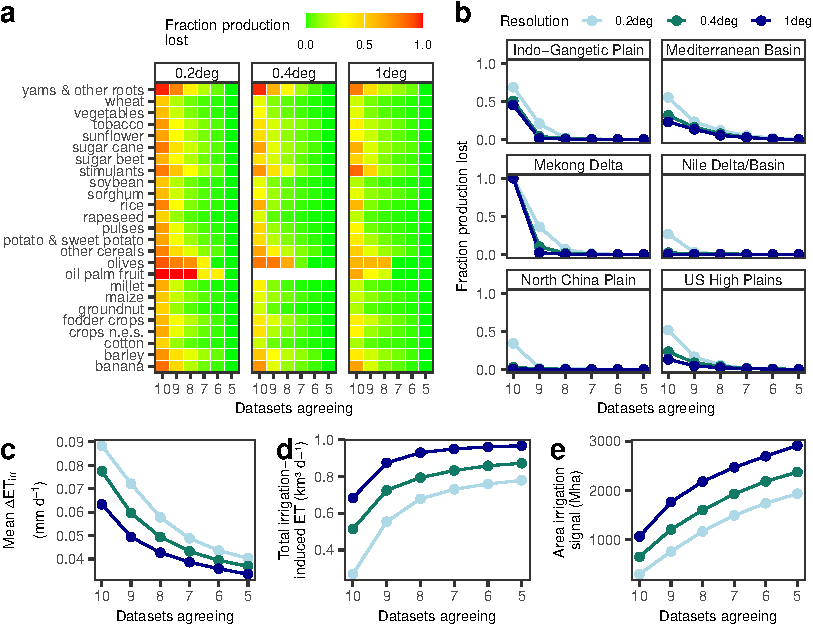
\includegraphics[keepaspectratio]{code_detectability_irrigated_areas_files/figure-latex/merge_ET_plots2-1.pdf}}

\newpage

\section{Final figures}\label{final-figures}

\begin{Shaded}
\begin{Highlighting}[]
\NormalTok{left }\OtherTok{\textless{}{-}} \FunctionTok{plot\_grid}\NormalTok{(plot\_uncertainty1, plot\_agreement1, }
\NormalTok{                  plot\_stacked }\SpecialCharTok{+} 
                    \FunctionTok{labs}\NormalTok{(}\AttributeTok{y =} \StringTok{"Fraction of cells"}\NormalTok{), }\AttributeTok{ncol =} \DecValTok{1}\NormalTok{, }\AttributeTok{labels =} \StringTok{"auto"}\NormalTok{)}
\end{Highlighting}
\end{Shaded}

\begin{verbatim}
## Warning in scale_x_log10(labels = label_log(digits = 2)): log-10 transformation introduced infinite values.
## log-10 transformation introduced infinite values.
## log-10 transformation introduced infinite values.
## log-10 transformation introduced infinite values.
\end{verbatim}

\begin{Shaded}
\begin{Highlighting}[]
\FunctionTok{plot\_grid}\NormalTok{(left, plot\_raster, }\AttributeTok{ncol =} \DecValTok{2}\NormalTok{, }\AttributeTok{rel\_widths =} \FunctionTok{c}\NormalTok{(}\FloatTok{0.3}\NormalTok{, }\FloatTok{0.7}\NormalTok{), }\AttributeTok{labels =} \FunctionTok{c}\NormalTok{(}\StringTok{""}\NormalTok{, }\StringTok{"d"}\NormalTok{))}
\end{Highlighting}
\end{Shaded}

\begin{verbatim}
## Warning: Raster pixels are placed at uneven horizontal intervals and will be shifted
## i Consider using `geom_tile()` instead.
\end{verbatim}

\begin{verbatim}
## Warning: Raster pixels are placed at uneven horizontal intervals and will be shifted
## i Consider using `geom_tile()` instead.
\end{verbatim}

\pandocbounded{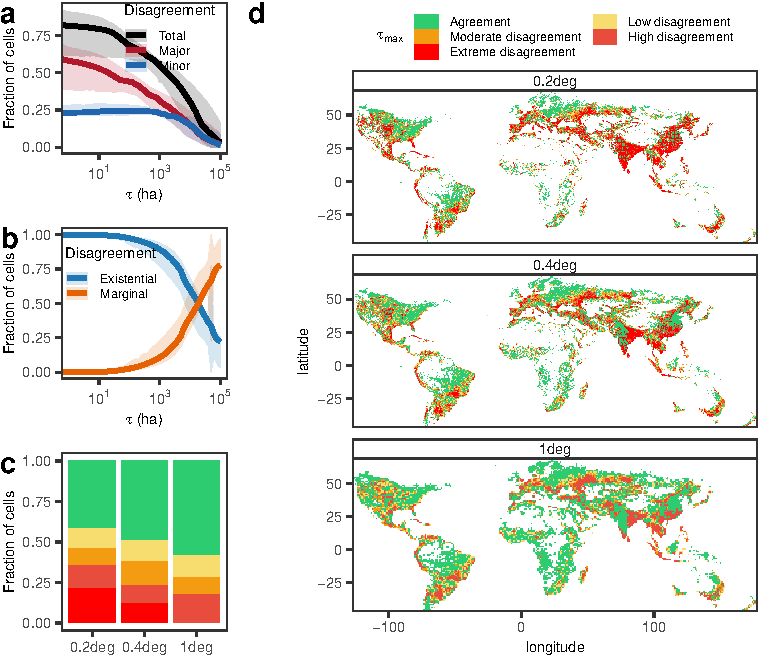
\includegraphics[keepaspectratio]{code_detectability_irrigated_areas_files/figure-latex/final_figure1-1.pdf}}

\begin{Shaded}
\begin{Highlighting}[]
\NormalTok{left }\OtherTok{\textless{}{-}} \FunctionTok{plot\_grid}\NormalTok{(plot\_uncertainty1, plot\_agreement1, }
\NormalTok{                  plot\_regime, }\AttributeTok{ncol =} \DecValTok{1}\NormalTok{, }\AttributeTok{labels =} \StringTok{"auto"}\NormalTok{)}
\end{Highlighting}
\end{Shaded}

\begin{verbatim}
## Warning in scale_x_log10(labels = label_log(digits = 2)): log-10 transformation introduced infinite values.
## log-10 transformation introduced infinite values.
## log-10 transformation introduced infinite values.
## log-10 transformation introduced infinite values.
\end{verbatim}

\begin{Shaded}
\begin{Highlighting}[]
\NormalTok{middle }\OtherTok{\textless{}{-}} \FunctionTok{plot\_grid}\NormalTok{(p1 }\SpecialCharTok{+} \FunctionTok{facet\_wrap}\NormalTok{(}\SpecialCharTok{\textasciitilde{}}\NormalTok{resolution, }\AttributeTok{ncol =} \DecValTok{1}\NormalTok{), }
\NormalTok{                    plot\_stacked }\SpecialCharTok{+}
                      \FunctionTok{labs}\NormalTok{(}\AttributeTok{y =} \StringTok{"Fraction of cells"}\NormalTok{), }
                    \AttributeTok{ncol =} \DecValTok{1}\NormalTok{, }\AttributeTok{rel\_heights =} \FunctionTok{c}\NormalTok{(}\FloatTok{0.7}\NormalTok{, }\FloatTok{0.3}\NormalTok{), }\AttributeTok{labels =} \FunctionTok{c}\NormalTok{(}\StringTok{"d"}\NormalTok{, }\StringTok{"e"}\NormalTok{))}
\FunctionTok{plot\_grid}\NormalTok{(left, middle, plot\_raster, }\AttributeTok{ncol =} \DecValTok{3}\NormalTok{, }\AttributeTok{rel\_widths =} \FunctionTok{c}\NormalTok{(}\FloatTok{0.26}\NormalTok{, }\FloatTok{0.26}\NormalTok{, }\FloatTok{0.48}\NormalTok{), }\AttributeTok{labels =} \FunctionTok{c}\NormalTok{(}\StringTok{""}\NormalTok{, }\StringTok{""}\NormalTok{, }\StringTok{"f"}\NormalTok{))}
\end{Highlighting}
\end{Shaded}

\begin{verbatim}
## Warning: Raster pixels are placed at uneven horizontal intervals and will be shifted
## i Consider using `geom_tile()` instead.
\end{verbatim}

\begin{verbatim}
## Warning: Raster pixels are placed at uneven horizontal intervals and will be shifted
## i Consider using `geom_tile()` instead.
\end{verbatim}

\pandocbounded{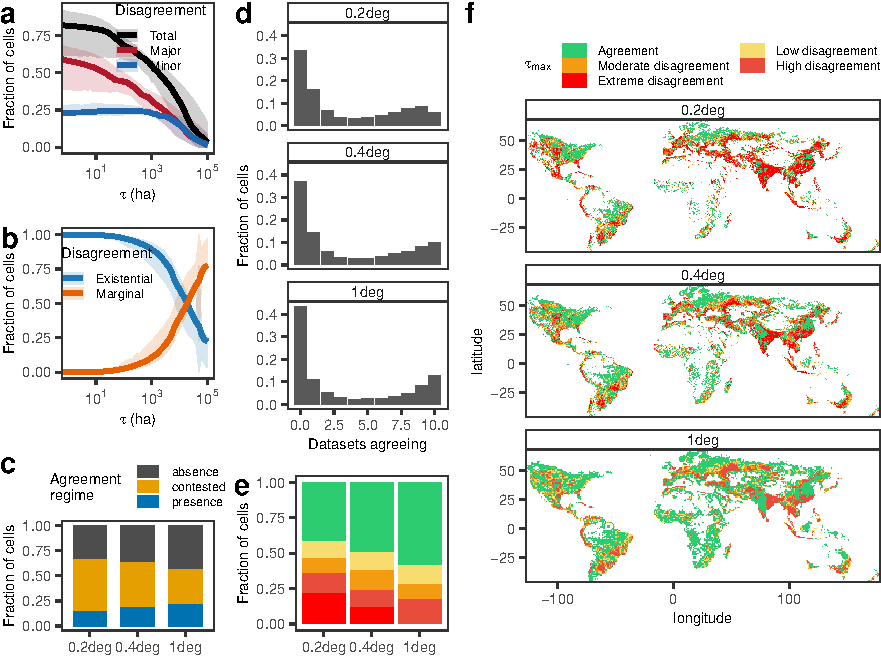
\includegraphics[keepaspectratio]{code_detectability_irrigated_areas_files/figure-latex/final_figure1_1-1.pdf}}

\begin{Shaded}
\begin{Highlighting}[]
\NormalTok{top }\OtherTok{\textless{}{-}} \FunctionTok{plot\_grid}\NormalTok{(plot\_indices1 }\SpecialCharTok{+} 
                   \FunctionTok{labs}\NormalTok{(}\AttributeTok{x =} \StringTok{""}\NormalTok{, }\AttributeTok{y =} \StringTok{"Fraction }\SpecialCharTok{\textbackslash{}n}\StringTok{ variance"}\NormalTok{) }\SpecialCharTok{+}
                   \FunctionTok{scale\_fill\_discrete}\NormalTok{(}\AttributeTok{name =} \StringTok{"Sobol\textquotesingle{} }\SpecialCharTok{\textbackslash{}n}\StringTok{ indices"}\NormalTok{) }\SpecialCharTok{+} 
                   \FunctionTok{theme}\NormalTok{(}\AttributeTok{legend.position =} \FunctionTok{c}\NormalTok{(}\FloatTok{0.4}\NormalTok{, }\FloatTok{0.7}\NormalTok{)), }
\NormalTok{                 a1 }\SpecialCharTok{+} \FunctionTok{labs}\NormalTok{(}\AttributeTok{x =} \StringTok{"exclusion"}\NormalTok{, }\AttributeTok{y =} \StringTok{"Fraction }\SpecialCharTok{\textbackslash{}n}\StringTok{ disagree"}\NormalTok{), }
\NormalTok{                 b1, c1, }\AttributeTok{ncol =} \DecValTok{4}\NormalTok{, }\AttributeTok{labels =} \FunctionTok{c}\NormalTok{(}\StringTok{"a"}\NormalTok{, }\StringTok{""}\NormalTok{, }\StringTok{""}\NormalTok{, }\StringTok{""}\NormalTok{), }
                 \AttributeTok{rel\_widths =} \FunctionTok{c}\NormalTok{(}\FloatTok{0.23}\NormalTok{, }\FloatTok{0.37}\NormalTok{, }\FloatTok{0.2}\NormalTok{, }\FloatTok{0.2}\NormalTok{))}
\end{Highlighting}
\end{Shaded}

\begin{verbatim}
## Scale for fill is already present.
## Adding another scale for fill, which will replace the existing scale.
\end{verbatim}

\begin{verbatim}
## Warning in scale_x_log10(labels = label_log(digits = 2)): log-10 transformation introduced infinite values.
## log-10 transformation introduced infinite values.
\end{verbatim}

\begin{verbatim}
## Warning: Removed 157 rows containing non-finite outside the scale range
## (`stat_summary_bin()`).
\end{verbatim}

\begin{Shaded}
\begin{Highlighting}[]
\NormalTok{top}
\end{Highlighting}
\end{Shaded}

\pandocbounded{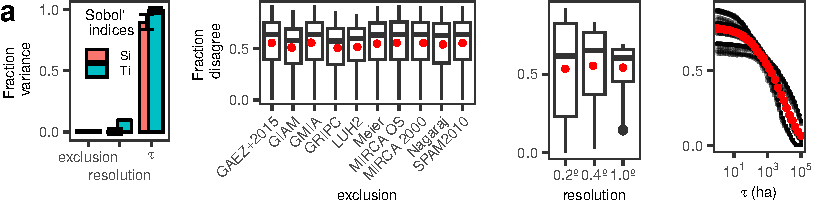
\includegraphics[keepaspectratio]{code_detectability_irrigated_areas_files/figure-latex/final_figure2-1.pdf}}

\begin{Shaded}
\begin{Highlighting}[]
\NormalTok{middle }\OtherTok{\textless{}{-}} \FunctionTok{plot\_grid}\NormalTok{(plot\_indices2 }\SpecialCharTok{+} 
                   \FunctionTok{labs}\NormalTok{(}\AttributeTok{x =} \StringTok{""}\NormalTok{, }\AttributeTok{y =} \StringTok{"Fraction }\SpecialCharTok{\textbackslash{}n}\StringTok{ variance"}\NormalTok{) }\SpecialCharTok{+}
                   \FunctionTok{scale\_fill\_discrete}\NormalTok{(}\AttributeTok{name =} \StringTok{""}\NormalTok{) }\SpecialCharTok{+} 
                   \FunctionTok{theme}\NormalTok{(}\AttributeTok{legend.position =} \StringTok{"none"}\NormalTok{), }
\NormalTok{                 a2 }\SpecialCharTok{+} \FunctionTok{labs}\NormalTok{(}\AttributeTok{x =} \StringTok{"exclusion"}\NormalTok{, }\AttributeTok{y =} \StringTok{"Fraction }\SpecialCharTok{\textbackslash{}n}\StringTok{ disagree"}\NormalTok{), }
\NormalTok{                 b2, c2, }\AttributeTok{ncol =} \DecValTok{4}\NormalTok{, }\AttributeTok{labels =} \FunctionTok{c}\NormalTok{(}\StringTok{"b"}\NormalTok{, }\StringTok{""}\NormalTok{, }\StringTok{""}\NormalTok{, }\StringTok{""}\NormalTok{), }
                 \AttributeTok{rel\_widths =} \FunctionTok{c}\NormalTok{(}\FloatTok{0.23}\NormalTok{, }\FloatTok{0.37}\NormalTok{, }\FloatTok{0.2}\NormalTok{, }\FloatTok{0.2}\NormalTok{))}
\end{Highlighting}
\end{Shaded}

\begin{verbatim}
## Scale for fill is already present.
## Adding another scale for fill, which will replace the existing scale.
\end{verbatim}

\begin{verbatim}
## Warning in scale_x_log10(labels = label_log(digits = 2)): log-10 transformation
## introduced infinite values.
\end{verbatim}

\begin{verbatim}
## Warning in scale_x_log10(labels = label_log(digits = 2)): log-10 transformation
## introduced infinite values.
\end{verbatim}

\begin{verbatim}
## Warning: Removed 157 rows containing non-finite outside the scale range
## (`stat_summary_bin()`).
\end{verbatim}

\begin{Shaded}
\begin{Highlighting}[]
\NormalTok{middle}
\end{Highlighting}
\end{Shaded}

\pandocbounded{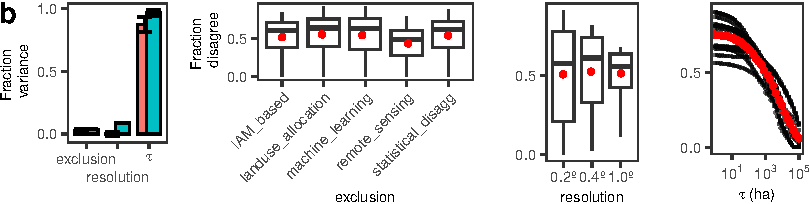
\includegraphics[keepaspectratio]{code_detectability_irrigated_areas_files/figure-latex/final_figure2-2.pdf}}

\begin{Shaded}
\begin{Highlighting}[]
\NormalTok{bottom }\OtherTok{\textless{}{-}} \FunctionTok{plot\_grid}\NormalTok{(plot\_indices3 }\SpecialCharTok{+} 
                   \FunctionTok{labs}\NormalTok{(}\AttributeTok{x =} \StringTok{""}\NormalTok{, }\AttributeTok{y =} \StringTok{"Fraction }\SpecialCharTok{\textbackslash{}n}\StringTok{ variance"}\NormalTok{) }\SpecialCharTok{+}
                   \FunctionTok{scale\_fill\_discrete}\NormalTok{(}\AttributeTok{name =} \StringTok{""}\NormalTok{) }\SpecialCharTok{+} 
                   \FunctionTok{theme}\NormalTok{(}\AttributeTok{legend.position =} \StringTok{"none"}\NormalTok{), }
\NormalTok{                 a3 }\SpecialCharTok{+} \FunctionTok{labs}\NormalTok{(}\AttributeTok{x =} \StringTok{"exclusion"}\NormalTok{, }\AttributeTok{y =} \StringTok{"Fraction }\SpecialCharTok{\textbackslash{}n}\StringTok{ disagree"}\NormalTok{), }
\NormalTok{                 b3, c3, d3, }\AttributeTok{ncol =} \DecValTok{5}\NormalTok{, }\AttributeTok{labels =} \FunctionTok{c}\NormalTok{(}\StringTok{"c"}\NormalTok{, }\StringTok{""}\NormalTok{, }\StringTok{""}\NormalTok{, }\StringTok{""}\NormalTok{, }\StringTok{""}\NormalTok{), }
                 \AttributeTok{rel\_widths =} \FunctionTok{c}\NormalTok{(}\FloatTok{0.22}\NormalTok{, }\FloatTok{0.34}\NormalTok{, }\FloatTok{0.16}\NormalTok{, }\FloatTok{0.15}\NormalTok{, }\FloatTok{0.15}\NormalTok{))}
\end{Highlighting}
\end{Shaded}

\begin{verbatim}
## Scale for fill is already present.
## Adding another scale for fill, which will replace the existing scale.
\end{verbatim}

\begin{verbatim}
## Warning in scale_x_log10(labels = label_log(digits = 2)): log-10 transformation
## introduced infinite values.
\end{verbatim}

\begin{verbatim}
## Warning in scale_x_log10(labels = label_log(digits = 2)): log-10 transformation
## introduced infinite values.
\end{verbatim}

\begin{verbatim}
## Warning: Removed 157 rows containing non-finite outside the scale range
## (`stat_summary_bin()`).
\end{verbatim}

\begin{Shaded}
\begin{Highlighting}[]
\NormalTok{bottom}
\end{Highlighting}
\end{Shaded}

\pandocbounded{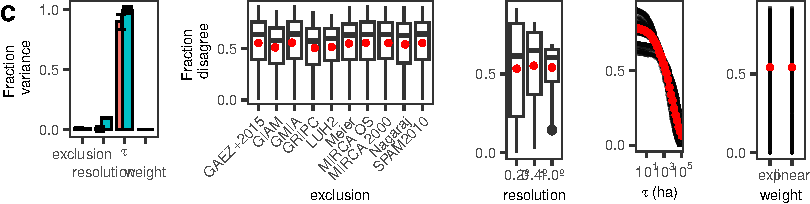
\includegraphics[keepaspectratio]{code_detectability_irrigated_areas_files/figure-latex/final_figure2-3.pdf}}

\begin{Shaded}
\begin{Highlighting}[]
\FunctionTok{plot\_grid}\NormalTok{(top, middle, bottom, }\AttributeTok{ncol =} \DecValTok{1}\NormalTok{)}
\end{Highlighting}
\end{Shaded}

\pandocbounded{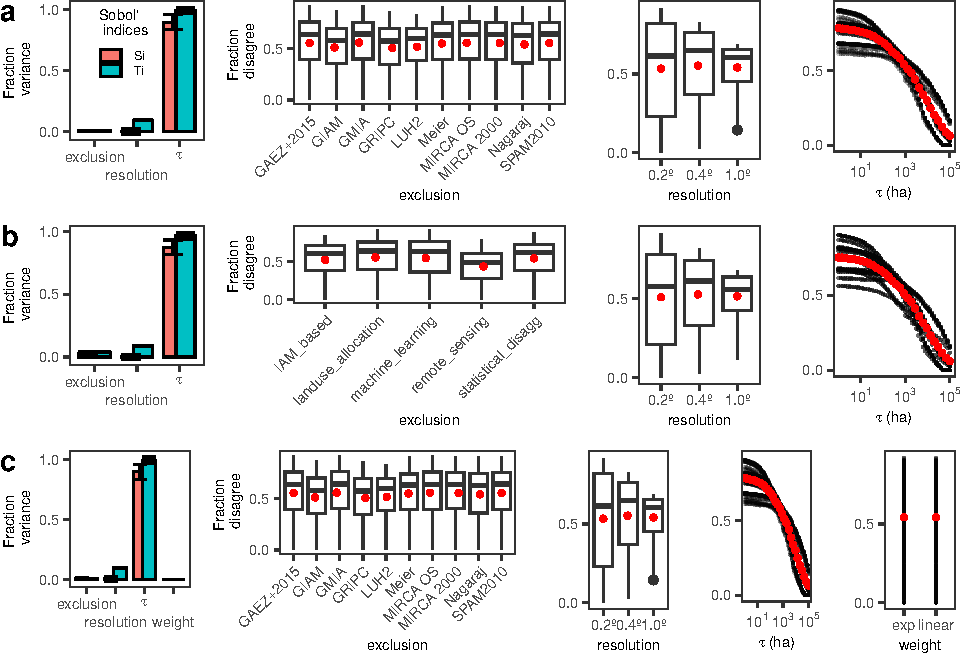
\includegraphics[keepaspectratio]{code_detectability_irrigated_areas_files/figure-latex/merge_all_sa-1.pdf}}

\section{Session information}\label{session-information}

\begin{Shaded}
\begin{Highlighting}[]
\CommentTok{\# SESSION INFORMATION \#\#\#\#\#\#\#\#\#\#\#\#\#\#\#\#\#\#\#\#\#\#\#\#\#\#\#\#\#\#\#\#\#\#\#\#\#\#\#\#\#\#\#\#\#\#\#\#\#\#\#\#\#\#\#\#\#\#}

\FunctionTok{sessionInfo}\NormalTok{()}
\end{Highlighting}
\end{Shaded}

\begin{verbatim}
## R version 4.5.2 (2025-10-31)
## Platform: aarch64-apple-darwin20
## Running under: macOS Tahoe 26.3.1
## 
## Matrix products: default
## BLAS:   /System/Library/Frameworks/Accelerate.framework/Versions/A/Frameworks/vecLib.framework/Versions/A/libBLAS.dylib 
## LAPACK: /Library/Frameworks/R.framework/Versions/4.5-arm64/Resources/lib/libRlapack.dylib;  LAPACK version 3.12.1
## 
## locale:
## [1] en_US.UTF-8/en_US.UTF-8/en_US.UTF-8/C/en_US.UTF-8/en_US.UTF-8
## 
## time zone: Europe/London
## tzcode source: internal
## 
## attached base packages:
## [1] stats     graphics  grDevices utils     datasets  methods   base     
## 
## other attached packages:
##  [1] benchmarkme_1.0.8   wesanderson_0.3.7   countrycode_1.6.1  
##  [4] sf_1.1-0            rnaturalearth_1.1.0 terra_1.8-93       
##  [7] here_1.0.2          sensobol_1.1.6      lubridate_1.9.4    
## [10] forcats_1.0.1       stringr_1.6.0       dplyr_1.1.4        
## [13] purrr_1.2.1         readr_2.2.0         tidyr_1.3.2        
## [16] tibble_3.3.1        ggplot2_4.0.1.9000  tidyverse_2.0.0    
## [19] cowplot_1.2.0.9000  scales_1.4.0        data.table_1.18.2.1
## 
## loaded via a namespace (and not attached):
##  [1] benchmarkmeData_1.0.4 gtable_0.3.6          xfun_0.55            
##  [4] lattice_0.22-7        tzdb_0.5.0            vctrs_0.7.1          
##  [7] tools_4.5.2           Rdpack_2.6.4          generics_0.1.4       
## [10] parallel_4.5.2        proxy_0.4-29          pkgconfig_2.0.3      
## [13] Matrix_1.7-4          KernSmooth_2.23-26    RColorBrewer_1.1-3   
## [16] S7_0.2.1              lifecycle_1.0.5       compiler_4.5.2       
## [19] farver_2.1.2          codetools_0.2-20      htmltools_0.5.9      
## [22] class_7.3-23          yaml_2.3.12           pillar_1.11.1        
## [25] classInt_0.4-11       iterators_1.0.14      foreach_1.5.2        
## [28] tidyselect_1.2.1      digest_0.6.39         stringi_1.8.7        
## [31] rprojroot_2.1.1       fastmap_1.2.0         grid_4.5.2           
## [34] cli_3.6.5             magrittr_2.0.4        e1071_1.7-17         
## [37] withr_3.0.2           timechange_0.3.0      httr_1.4.8           
## [40] rmarkdown_2.30        otel_0.2.0            hms_1.1.4            
## [43] evaluate_1.0.5        knitr_1.51            rbibutils_2.4        
## [46] doParallel_1.0.17     rlang_1.1.7           Rcpp_1.1.1           
## [49] glue_1.8.0            DBI_1.3.0             rstudioapi_0.17.1    
## [52] R6_2.6.1              units_1.0-0
\end{verbatim}

\begin{Shaded}
\begin{Highlighting}[]
\DocumentationTok{\#\# Return the machine CPU {-}{-}{-}{-}{-}{-}{-}{-}{-}{-}{-}{-}{-}{-}{-}{-}{-}{-}{-}{-}{-}{-}{-}{-}{-}{-}{-}{-}{-}{-}{-}{-}{-}{-}{-}{-}{-}{-}{-}{-}{-}{-}{-}{-}{-}{-}{-}{-}{-}{-}{-}{-}{-}}

\FunctionTok{cat}\NormalTok{(}\StringTok{"Machine:     "}\NormalTok{); }\FunctionTok{print}\NormalTok{(}\FunctionTok{get\_cpu}\NormalTok{()}\SpecialCharTok{$}\NormalTok{model\_name)}
\end{Highlighting}
\end{Shaded}

\begin{verbatim}
## Machine:
\end{verbatim}

\begin{verbatim}
## [1] "Apple M1 Max"
\end{verbatim}

\begin{Shaded}
\begin{Highlighting}[]
\DocumentationTok{\#\# Return number of true cores {-}{-}{-}{-}{-}{-}{-}{-}{-}{-}{-}{-}{-}{-}{-}{-}{-}{-}{-}{-}{-}{-}{-}{-}{-}{-}{-}{-}{-}{-}{-}{-}{-}{-}{-}{-}{-}{-}{-}{-}{-}{-}{-}{-}{-}{-}{-}{-}{-}}

\FunctionTok{cat}\NormalTok{(}\StringTok{"Num cores:   "}\NormalTok{); }\FunctionTok{print}\NormalTok{(parallel}\SpecialCharTok{::}\FunctionTok{detectCores}\NormalTok{(}\AttributeTok{logical =} \ConstantTok{FALSE}\NormalTok{))}
\end{Highlighting}
\end{Shaded}

\begin{verbatim}
## Num cores:
\end{verbatim}

\begin{verbatim}
## [1] 10
\end{verbatim}

\begin{Shaded}
\begin{Highlighting}[]
\DocumentationTok{\#\# Return number of threads {-}{-}{-}{-}{-}{-}{-}{-}{-}{-}{-}{-}{-}{-}{-}{-}{-}{-}{-}{-}{-}{-}{-}{-}{-}{-}{-}{-}{-}{-}{-}{-}{-}{-}{-}{-}{-}{-}{-}{-}{-}{-}{-}{-}{-}{-}{-}{-}{-}{-}{-}}

\FunctionTok{cat}\NormalTok{(}\StringTok{"Num threads: "}\NormalTok{); }\FunctionTok{print}\NormalTok{(parallel}\SpecialCharTok{::}\FunctionTok{detectCores}\NormalTok{(}\AttributeTok{logical =} \ConstantTok{FALSE}\NormalTok{))}
\end{Highlighting}
\end{Shaded}

\begin{verbatim}
## Num threads:
\end{verbatim}

\begin{verbatim}
## [1] 10
\end{verbatim}

\end{document}
